\chapter{Grundlagen und Stand der Technik}
\label{ch:state_of_the_art}

% NEU GEFASST am 15.09.2026 nach dem Absatzplan im Sammelmodus.
% Befunde B40, B41, G1. Definition der kurativen Vorhaltung steht in 1.2, Subjekte nach Stilregel 10.
% Alte Fassung, nicht wieder aufnehmen:
%Ein Marktmechanismus für die kurative Vorhaltung trifft auf einen bestehenden technischen, rechtlichen und marktlichen Rahmen.
%Dieses Kapitel legt zunächst die konzeptionellen, physikalischen und regulatorischen Grundlagen der kurativen Systemführung dar und begründet dabei, welche Technologie als kurativer Akteur in Betracht kommt.
%Anschließend stellt es den Marktrahmen mit seinen Dispatchmodellen, Marktzeithorizonten und Systemdienstleistungen dar.
%Zuletzt untersucht es, ob sich eine der bestehenden Vergütungslogiken auf die kurative Vorhaltung anwenden lässt und gegen welche Vermarktungswege eine solche Vorhaltung anträte.
In diesem Kapitel werden zunächst die konzeptionellen, physikalischen und regulatorischen Grundlagen der kurativen Systemführung dargelegt, und daraus wird begründet, welche Technologie als kurativer Akteur in Betracht kommt.
Anschließend wird der Marktrahmen mit seinen Dispatchmodellen, Marktzeithorizonten und Systemdienstleistungen dargestellt.
Zuletzt wird geprüft, ob sich eine der bestehenden Vergütungslogiken auf die kurative Vorhaltung anwenden lässt und gegen welche Vermarktungswege eine solche Vorhaltung anträte.

\section{Kurative Systemführung}
\label{sec:curative_basics}

% NEU GEFASST am 15.09.2026 nach dem Absatzplan im Sammelmodus.
% Befunde B43, B46, V4, V11, G2 bis G6. Ausfallvariante, Ausfallvariantenliste, Befund und Engpass definiert, Vorverweise und Abschnittsankuendigung gestrichen, aktivierbar und Aktivierungszeiten ersetzt.
% Alte Fassung, nicht wieder aufnehmen:
%Engpassmanagement bezeichnet die Gesamtheit der Maßnahmen, mit denen ein Netzbetreiber eine drohende oder bereits eingetretene Überlastung von Betriebsmitteln beseitigt.
%Zu diesen Maßnahmen zählt der Redispatch, also die gezielte Anpassung der Einspeisung einzelner Anlagen zur Behebung des Engpasses \cite{bundesministerium_der_justiz_energiewirtschaftsgesetz_2025}.
%Den rechtlichen Rahmen dafür stellt Abschnitt \ref{sec:legal_framework} dar.
%Maßstab für die Frage, wann ein Eingriff erforderlich ist, ist das \mbox{(N-1)-Kriterium}.
%Der sichere Betrieb des deutschen Übertragungsnetzes ist auf die Einhaltung dieses Kriteriums im Normalzustand ausgelegt.
%Es ist in der europäischen Leitlinie für den Übertragungsnetzbetrieb verbindlich definiert als \glqq{}die Regel, wonach die nach dem Auftreten eines Ausfalls weiter in Betrieb befindlichen Betriebsmittel innerhalb der Regelzone eines \ac{ÜNB} in der Lage sind, sich an die neue Betriebssituation anzupassen, ohne betriebliche Sicherheitsgrenzwerte zu überschreiten\grqq{} \cite{europaische_kommission_verordnung_2017}.
%Die Art und Weise, wie \ac{ÜNB} dieses Kriterium erfüllen, unterscheidet sich je nach Systemführungskonzept.
%Die kurative Systemführung ist dabei eine Form der Engpassbewirtschaftung, die das \mbox{(N-1)-Kriterium} nicht präventiv, sondern durch vordefinierte Systemautomatiken oder manuell aktivierbare Gegenmaßnahmen nach Eintreten des Fehlerfalles sicherstellt \cite{innosys_2030_gesamtverbund_innovationen_2021}.
%Der Maßnahmenraum kurativer Eingriffe und die Anforderungen an ihre Aktivierungszeiten sind im Verbundprojekt InnoSys~2030 systematisiert worden \cite{innosys_2030_gesamtverbund_innovationen_2021}.
%Daran anschließend liegen Arbeiten zur Integration kurativer Maßnahmen in die Betriebsplanung vor \cite{leeuwen_integration_2020}.
%Dieser Abschnitt stellt auf dieser Grundlage die Abgrenzung gegenüber der präventiven Systemführung, den Prozessablauf mit seinen Zeitanforderungen, die in Betracht kommenden Technologien sowie den rechtlichen Rahmen mit den offenen Umsetzungsfragen dar.
% ANGEBUNDEN am 19.09.2026, Kommentar des Verfassers: der Abschnitt heisst kurative Systemfuehrung und nannte sie im ersten Absatz nicht, und der Redispatch-Satz stand ohne Aufgabe. Alte Fassung:
%Engpassmanagement bezeichnet die Gesamtheit der Maßnahmen, mit denen ein Netzbetreiber eine drohende oder bereits eingetretene Überlastung von Betriebsmitteln wie Leitungen und Transformatoren beseitigt.
%Zu diesen Maßnahmen zählt der Redispatch, also die angeordnete Anpassung der Einspeisung einzelner Anlagen zur Behebung des Engpasses \cite{bundesministerium_der_justiz_energiewirtschaftsgesetz_2025}.
Die kurative Systemführung ist eine Form des Engpassmanagements, also der Gesamtheit der Maßnahmen, mit denen ein Netzbetreiber eine drohende oder bereits eingetretene Überlastung von Betriebsmitteln wie Leitungen und Transformatoren beseitigt.
% VORRANG BENANNT am 19.09.2026, Kommentar des Verfassers: der Redispatch ist die gegenwaertig praesenteste Art, Engpaesse zu bewirtschaften. Zurueckhaltend formuliert nach Stilregel 8, weil die BNetzA-Daten das Massnahmenvolumen des gesamten Netzengpassmanagements ausweisen und nicht den Anteil des Redispatch. Alte Fassung:
%Das Engpassmanagement stützt sich dabei auf den Redispatch, also die angeordnete Anpassung der Einspeisung einzelner Anlagen zur Behebung des Engpasses \cite{bundesministerium_der_justiz_energiewirtschaftsgesetz_2025}.
Das Engpassmanagement stützt sich heute überwiegend auf den Redispatch, also auf die angeordnete Anpassung der Einspeisung einzelner Anlagen zur Behebung des Engpasses \cite{bundesministerium_der_justiz_energiewirtschaftsgesetz_2025}.
Ob ein Engpass vorliegt, ermittelt der \ac{ÜNB} in der Netzsicherheitsrechnung, in der er für den erwarteten Netzzustand den Ausfall jedes einzelnen Betriebsmittels durchrechnet.
Ein solcher angenommener Ausfall heißt Ausfallvariante, und die Menge der durchgerechneten Ausfälle bildet die Ausfallvariantenliste \cite{europaische_kommission_verordnung_2017}.
Überschreitet die Belastung eines Betriebsmittels bei Verfügbarkeit aller Betriebsmittel oder in einer Ausfallvariante den betrieblichen Sicherheitsgrenzwert, liegt ein Befund vor, und ein Engpass ist ein Netzzustand, in dem ein solcher Befund besteht.
Ein Eingriff ist damit erforderlich, sobald die Netzsicherheitsrechnung einen Befund liefert.

Der Maßstab, gegen den die Netzsicherheitsrechnung prüft, ist das \mbox{(N-1)-Kriterium}, auf dessen Einhaltung im Normalzustand der sichere Betrieb des deutschen Übertragungsnetzes ausgelegt ist.
Die europäische Leitlinie für den Übertragungsnetzbetrieb definiert das Kriterium als \glqq{}die Regel, wonach die nach dem Auftreten eines Ausfalls weiter in Betrieb befindlichen Betriebsmittel innerhalb der Regelzone eines \ac{ÜNB} in der Lage sind, sich an die neue Betriebssituation anzupassen, ohne betriebliche Sicherheitsgrenzwerte zu überschreiten\grqq{} \cite{europaische_kommission_verordnung_2017}.
Wie die \ac{ÜNB} das Kriterium erfüllen, unterscheidet sich nach dem Systemführungskonzept: Die präventive Systemführung stellt es vor dem Fehlerfall durch Anpassung der Fahrpläne sicher, die kurative Systemführung durch vordefinierte Gegenmaßnahmen nach Eintreten des Fehlerfalles.
% R-11 am 18.09.2026, Kontrolle durch Fable, Entscheidung des Verfassers: der Satz steht jetzt als Ueberleitung am Anfang von 2.1.1. Alte Fassung:
%Das Verbundprojekt InnoSys~2030 hat den Maßnahmenraum kurativer Eingriffe und die Anforderungen an ihre Umsetzungszeiten systematisiert, und daran anschließende Arbeiten behandeln die Integration kurativer Maßnahmen in die Betriebsplanung \cite{innosys_2030_gesamtverbund_innovationen_2021, leeuwen_integration_2020}.
% R-11 am 18.09.2026, Kontrolle durch Fable, Entscheidung des Verfassers: der Satz steht jetzt als Ueberleitung am Anfang von 2.1.1. Alte Fassung:
%Die drei Klassen der Umsetzungszeit aus InnoSys~2030 bilden im Folgenden die Grundlage für die Anforderungen an den kurativen Akteur.

\subsection{Präventive und kurative Systemführung im Engpassmanagement}
\label{sec:prev_vs_cur}

% UMSTELLUNG DES ABSCHNITTS am 19.09.2026, Kommentar des Verfassers: "der aufbau gefaellt mir
% noch nicht ganz. ich wuerde gerne erst mit praeventiv anfangen das erklaeren, dann kurativ".
% Die Absatzfolge lautet jetzt: praeventiver Regelfall, Kosten und Grenze des praeventiven
% Vorgehens in drei Absaetzen, Ueberleitung zum kurativen Ansatz, Netzzustand, thermische
% Traegheit mit PATL und TATL, Abbildung, kurative Auspraegungen, Jahressimulationen, InnoSys.
% Vorher standen der kurative Teil und die Grenzwerte in den Absaetzen 1 und 2 vor dem
% praeventiven Teil. Kein Satz ist gestrichen, die Absatzgrenzen sind neu gesetzt. Die
% Formulierungen folgen dem Textblock des Verfassers vom 19.09.2026, soweit Stilregel 17 sie
% traegt, lange Satzketten sind geteilt.
% ZWEITE UMSTELLUNG am 19.09.2026, Kommentar des Verfassers zum Absatz Kosten und Grenze:
% "den ganzen absatz find ich ja ansich gut aber wuerde das nicht besser ans ende passen, wenn
% man erklaert hat was kurativ und was praeventiv ist und die probleme von praeventiv anspricht
% und kurativ dann dort einordnet?". Der Absatz steht deshalb hinter der Erklaerung beider
% Ansaetze und unmittelbar vor dem Absatz, der die kurative Systemfuehrung an der Marge und am
% Planungshorizont einordnet. Die Absatzfolge lautet jetzt: praeventiver Regelfall, Unterschied
% im Zeitpunkt mit Netzzustand, thermische Traegheit mit PATL und TATL und Abbildung, Kosten und
% Grenze des praeventiven Vorgehens, kurative Auspraegungen, Einsparpotenzial und InnoSys 2030.

% NEU GEFASST am 15.09.2026 nach dem Absatzplan im Sammelmodus.
% Befunde B45, G10, G11, Q1, Q14. Praeventiver Redispatch als Regelfall genannt, Stufung gekuerzt, Vorteil und Optimalfall verbunden.
% Alte Fassung, nicht wieder aufnehmen:
%Der präventive Ansatz stellt (N-1)-Sicherheit her, indem er die zulässige Vorauslastung der Betriebsmittel unterhalb der \ac{PATL} begrenzt und die dafür erforderlichen Anpassungen bereits in der Einsatzplanung anordnet.
%Grundlage dafür ist eine gestufte Betriebsplanung, die den Netzzustand mit abnehmendem zeitlichen Vorlauf zunehmend genau abbildet.
%Die \ac{SOGL} verpflichtet die \ac{ÜNB}, abgestimmte Netzmodelle für den Jahres-, den Vortages- und den untertägigen Horizont zu erstellen, sie untereinander auszutauschen und darauf Betriebssicherheitsanalysen durchzuführen \cite{europaische_kommission_verordnung_2017}.
%Die deutschen Redispatchprozesse lehnen sich an diese Stufung an und führen den erforderlichen Eingriff sukzessive durch, indem jede Planungsstufe den zu ihrem Zeitpunkt erkennbaren Engpass adressiert und die folgende Stufe die verbleibende Abweichung übernimmt \cite{leeuwen_integration_2020}.
%Der Vorteil dieses Vorgehens liegt in der Planungssicherheit, denn Engpässe werden so früh wie möglich erkannt und im Fehlerfall sind keine reaktiven Eingriffe erforderlich.
%Im Optimalfall hat die letzte Planungsstufe den Engpass vollständig aufgelöst, sodass bis zum Lieferzeitpunkt kein weiterer Eingriff mehr erforderlich ist.
Der präventive Ansatz bildet heute den Regelfall und ordnet die erforderlichen Anpassungen, in der Regel präventiven Redispatch, bereits in der Einsatzplanung an.
Grundlage dafür ist eine gestufte Betriebsplanung, in der die \ac{SOGL} die \ac{ÜNB} verpflichtet, abgestimmte Netzmodelle für den Jahres-, den Vortages- und den untertägigen Horizont zu erstellen und darauf Betriebssicherheitsanalysen durchzuführen \cite{europaische_kommission_verordnung_2017}.
Die deutschen Redispatchprozesse lehnen sich an diese Stufung an, indem jede Planungsstufe den zu ihrem Zeitpunkt erkennbaren Engpass behebt und die folgende Stufe die verbleibende Abweichung übernimmt \cite{leeuwen_integration_2020}.
% SATZLAENGE am 15.09.2026, Stilregel 17, alte Fassung als Kommentar:
%Der Vorteil liegt in der Planungssicherheit, denn Engpässe werden so früh wie möglich erkannt, und im Optimalfall hat die letzte Planungsstufe den Engpass vollständig aufgelöst, sodass im Fehlerfall kein reaktiver Eingriff mehr nötig ist.
Der Vorteil liegt in der Planungssicherheit, denn Engpässe werden so früh wie möglich erkannt.
Im Optimalfall hat die letzte Planungsstufe den Engpass vollständig aufgelöst, sodass im Fehlerfall kein reaktiver Eingriff mehr nötig ist.

% NEUER ABSATZ am 19.09.2026, Umstellung: die Ueberleitung vom praeventiven zum kurativen Teil.
% Der Verfasser hat den am 18.09.2026 als S-05 gestrichenen Satz in seinem Textblock wieder
% aufgenommen, weil er als Scharnier zwischen beiden Teilen traegt. Die Streichung ist damit
% zurueckgenommen. Der Satz ist nach Stilregel 17 in drei Saetze geteilt. Der Ausdruck
% Ueberlastintervall aus dem Textblock ist durch den verbindlichen Begriff zulaessige
% Ueberlastdauer ersetzt, CLAUDE.md Abschnitt 5. Der Vermerk der Streichung:
% S-05 am 18.09.2026, Kontrolle durch Fable, Entscheidung des Verfassers: gestrichen, die Aussage traegt 2.1 Absatz 3. Gestrichener Satz: Alte Fassung:
%Der Unterschied beider Konzepte liegt damit im Zeitpunkt des Eingriffs: Der präventive Ansatz bewirtschaftet den Engpass im Voraus, indem er ihn durch Anpassung der Fahrpläne gar nicht erst entstehen lässt, während der kurative Ansatz den bereits eingetretenen Engpass innerhalb des zulässigen Überlastintervalls behebt.
% Die beiden Saetze zur Entlastungsmassnahme standen bis zum 19.09.2026 am Anfang des Abschnitts.
Der Unterschied beider Ansätze liegt damit im Zeitpunkt des Eingriffs.
Der präventive Ansatz bewirtschaftet den Engpass im Voraus, indem er ihn durch Anpassung der Fahrpläne gar nicht erst entstehen lässt.
Der kurative Ansatz behebt dagegen den bereits eingetretenen Engpass innerhalb der zulässigen Überlastdauer.
% GESTRICHEN am 19.09.2026, Kommentar des Verfassers: "was bringt mir die info? also wenn ich
% einfach nur sagen will das kurativ im engpassmanagement eingesetzt wird habe ich das ja schon
% mehrfach getan". Eigenstaendige Pruefung: beide Saetze fuehren den Nachweis, dass der kurative
% Betrieb der Leitlinie entspricht. Denselben Nachweis fuehrt 2.1.5 Rechtlicher Rahmen
% vollstaendig und in drei Schritten, dort steht die Aufzaehlung der Massnahmenarten mit einem
% eigenen Zweck, naemlich der Unterscheidung netzbezogen gegen marktbezogen, und dort steht auch
% der Satz zum fehlenden Zeitpunktvorbehalt mit dem woertlichen Zitat der Leitlinie. 2.1.5
% verweist fuer die Zurechnung zum Netzzustand auf diesen Abschnitt zurueck, die Arbeitsteilung
% bleibt also erhalten. Die Definition der Entlastungsmassnahme ist in den Satz gewandert, der sie
% braucht. Gestrichene Saetze:
%Kurative Maßnahmen sind Entlastungsmaßnahmen im Sinne der \ac{SOGL}, also Maßnahmen zur Behebung einer Grenzwertverletzung, denn die Leitlinie nennt als deren Arten unter anderem den Redispatch, Topologieschaltmaßnahmen und die Anpassung der Wirkleistungsflüsse von \ac{HGÜ}-Systemen.
%An den Zeitpunkt ihres Einsatzes knüpft die Leitlinie keine Bedingung.
% ABSAETZE VERBUNDEN am 19.09.2026, Vorgabe des Verfassers: "mir werden hier viel zu viel absaetze gemacht ... ein absatz sollte eigentlich mal mindestens eine halbe seite lang sein". Die Leerzeile stand hier bis zum 19.09.2026. Die Ueberleitung und der Netzzustand tragen eine Kernaussage, naemlich dass der kurative Eingriff den Normalzustand wahrt.
% NEU GEFASST am 15.09.2026 nach dem Absatzplan im Sammelmodus.
% Befunde B42, B43, B44, G7, G8, G9, Q13, V4. Konzepte beim Namen genannt, Not- und Blackoutzustand entfallen, Fussnote fuer die Bezeichnungen, zwei Absaetze.
% Alte Fassung, nicht wieder aufnehmen:
%Zur Einordnung beider Ansätze eignet sich das in Art.\,18 \ac{SOGL} verankerte Vier-Zustands-Modell des Netzes mit Normal-, Gefährdungs-, Not- und Blackout-Zustand \cite{europaische_kommission_verordnung_2017}.
%Im Normalbetrieb sind alle Betriebsmittel innerhalb ihrer Grenzwerte belastet und das System ist (N-1)-sicher.
%Der Gefährdungszustand tritt ein, wenn die Grenzwerte zwar eingehalten werden, ein Ausfall aus der Ausfallvariantenliste aber zu einer Überschreitung führen würde, selbst wenn Entlastungsmaßnahmen aktiviert werden.
%Der Notzustand ist demgegenüber dadurch gekennzeichnet, dass mindestens ein betrieblicher Sicherheitsgrenzwert nicht mehr eingehalten wird.
%Der Blackout-Zustand beschreibt schließlich den vollständigen oder teilweisen Zusammenbruch der Versorgung, an den sich der Netzwiederaufbau anschließt.
%Maßgeblich für die Zuordnung ist dabei nicht der bereits eingetretene Ausfall, sondern die verbleibende Ausfallfestigkeit, denn die Verordnung rechnet die Wirkung der verfügbaren Entlastungsmaßnahmen dem Netzzustand zu \cite{europaische_kommission_verordnung_2017}.
%Wird auch jeder weitere Ausfall der Ausfallvariantenliste unter Aktivierung von Entlastungsmaßnahmen ohne Überschreitung der Grenzwerte beherrscht, bleibt das Netz im Normalzustand, andernfalls ist es gefährdet.
%Kurative Maßnahmen sind Entlastungsmaßnahmen in diesem Sinne, denn die Verordnung nennt als deren Arten unter anderem den Redispatch, Topologieschaltmaßnahmen und die Anpassung der Wirkleistungsflüsse von \ac{HGÜ}-Systemen und knüpft an den Zeitpunkt ihrer Aktivierung keine Bedingung.
%Die Nutzung der vorübergehend zulässigen Überlast führt damit für sich genommen nicht aus dem Normalzustand heraus, weil sie innerhalb der Grenzwerte liegt, während die Ausfallfestigkeit gegenüber dem nächsten Ausfall im Einzelfall zu prüfen ist.
%Der Unterschied beider Ansätze liegt damit im Zeitpunkt des Eingriffs.
%Der präventive Ansatz bewirtschaftet den Engpass im Voraus, indem er ihn durch Anpassung der Fahrpläne gar nicht erst entstehen lässt, während der kurative Ansatz den bereits eingetretenen Engpass innerhalb des zulässigen Überlastintervalls behebt.
%Physikalische Grundlage hierfür ist die thermische Trägheit von Betriebsmitteln, die kurzfristig höhere Strombelastungen tolerieren, als im Dauerbetrieb zulässig sind, und damit ein Zeitfenster für die Aktivierung kurativer Gegenmaßnahmen eröffnen.
%Die physikalische Ausprägung dieses Zeitfensters konkretisiert die \ac{SOGL} über die betrieblichen Sicherheitsgrenzwerte, die jeder \ac{ÜNB} für jedes Betriebsmittel festzulegen hat.
%Die \ac{PATL} ist dabei die Strombelastbarkeit, die ein Betriebsmittel ohne zeitliche Begrenzung führen kann.
%Die \ac{TATL} ist eine darüber liegende Strombelastbarkeit, die nur vorübergehend zulässig ist, wobei zu jeder Höhe der Überlast eine zugehörige zulässige Dauer festzulegen ist.
%Die Verordnung selbst verwendet diese beiden Bezeichnungen nicht, sondern spricht von den Grenzwerten für den Strom hinsichtlich der thermischen Belastbarkeit einschließlich vorübergehend zulässiger Überlastungen \cite{europaische_kommission_verordnung_2017}.
%Der Abstand zwischen beiden Grenzwerten und die zugehörige Dauer bestimmen damit, wie viel Zeit für eine kurative Gegenmaßnahme zur Verfügung steht.
%Abbildung \ref{fig:preventiv_kurativ} veranschaulicht den grundlegenden Unterschied zwischen beiden Systemführungsansätzen anhand der Betriebsmittelbelastung im Fehlerfall.
%Im präventiven Betrieb wird die Vorauslastung so weit begrenzt, dass die Belastung auch nach dem Ausfall unterhalb der \ac{PATL} bleibt.
%Die kurative Systemführung erlaubt hingegen eine höhere Vorauslastung bis zur \ac{PATL} im Normalbetrieb, nutzt nach Eintreten des Fehlerfalles das durch die \ac{TATL} definierte Zeitfenster und behebt den Engpass durch eine gezielte Gegenmaßnahme, bevor die transiente Stromtragfähigkeit überschritten wird.
% I-06 am 17.09.2026, Kontrolle durch Fable, Entscheidung des Verfassers: Art. 3 Nr. 36 der Leitlinie zaehlt fuenf Netzzustaende auf, Art. 18 Abs. 5 definiert den Netzwiederaufbau-Zustand. Alte Fassung:
%Zur Einordnung der präventiven und der kurativen Systemführung eignet sich das in Art.\,18 \ac{SOGL} verankerte Vier-Zustands-Modell des Netzes mit Normal-, Gefährdungs-, Not- und Blackout-Zustand, von denen die beiden letzten eine eingetretene Grenzwertverletzung und den Zusammenbruch der Versorgung bezeichnen und für die Einordnung keine Rolle spielen \cite{europaische_kommission_verordnung_2017}.
% R-12 am 18.09.2026, Kontrolle durch Fable, Entscheidung des Verfassers: These nach vorn und Satz geteilt, Stilregeln 1 und 17. Alte Fassung:
%Zur Einordnung der präventiven und der kurativen Systemführung eignet sich das in Art.\,18 \ac{SOGL} verankerte Fünf-Zustands-Modell des Netzes mit Normal-, Gefährdungs-, Not-, Blackout- und Netzwiederaufbau-Zustand, von denen die letzten drei eine eingetretene Grenzwertverletzung, den Zusammenbruch der Versorgung und die Wiederherstellung danach bezeichnen und für die Einordnung keine Rolle spielen \cite{europaische_kommission_verordnung_2017}.
% R-11 am 18.09.2026, Kontrolle durch Fable: die beiden Saetze zu InnoSys 2030 standen am Ende der Einleitung von 2.1 und leiten jetzt diesen Abschnitt ein.
% AUFTAKT GESTRICHEN am 19.09.2026, Kommentar des Verfassers: mit InnoSys zu starten ist holprig und folgt nicht dem vorigen Absatz. Was das Projekt erarbeitet hat, steht jetzt im letzten Absatz von 2.1.1. Der Vorverweis auf die drei Klassen faellt weg, sie werden in 2.1.2 eingefuehrt. Gestrichene Saetze:
%Das Verbundprojekt InnoSys~2030 hat den Maßnahmenraum kurativer Eingriffe und die Anforderungen an ihre Umsetzungszeiten systematisiert, und daran anschließende Arbeiten behandeln die Integration kurativer Maßnahmen in die Betriebsplanung \cite{innosys_2030_gesamtverbund_innovationen_2021, leeuwen_integration_2020}.
%Die drei Klassen der Umsetzungszeit aus InnoSys~2030 bilden im Folgenden die Grundlage für die Anforderungen an den kurativen Akteur.
% ABSAETZE VERBUNDEN am 19.09.2026, Vorgabe des Verfassers: "mir werden hier viel zu viel absaetze gemacht ... ein absatz sollte eigentlich mal mindestens eine halbe seite lang sein". Die Leerzeile stand hier bis zum 19.09.2026. Zweite Leerzeile derselben Verbindung, die Kommentare dazwischen bleiben stehen.
% FOLGERUNG VORAN am 19.09.2026, Kommentar des Verfassers: der Absatz holte zu weit aus, die Folgerung steht jetzt am Anfang und wird danach begruendet. Zehn Saetze werden acht, die Aufzaehlung der fuenf Zustaende und der Satz zu den letzten drei Zustaenden entfallen. Alte Fassung:
%Kurative Maßnahmen sind Entlastungsmaßnahmen im Sinne der \ac{SOGL}, denn die Leitlinie nennt als deren Arten unter anderem den Redispatch, Topologieschaltmaßnahmen und die Anpassung der Wirkleistungsflüsse von \ac{HGÜ}-Systemen.
%An den Zeitpunkt ihres Einsatzes knüpft die Leitlinie keine Bedingung.
%Zur Einordnung der präventiven und der kurativen Systemführung eignet sich das in Art.\,18 \ac{SOGL} verankerte Fünf-Zustands-Modell des Netzes mit Normal-, Gefährdungs-, Not-, Blackout- und Netzwiederaufbau-Zustand \cite{europaische_kommission_verordnung_2017}.
%Die letzten drei Zustände bezeichnen eine eingetretene Grenzwertverletzung, den Zusammenbruch der Versorgung und die Wiederherstellung danach und spielen für die Einordnung keine Rolle.
%Im Normalzustand sind alle Betriebsmittel innerhalb ihrer Grenzwerte belastet und das System ist (N-1)-sicher.
% R-12 am 18.09.2026, Kontrolle durch Fable, Entscheidung des Verfassers: Satz geteilt, Stilregel 17. Alte Fassung:
%Der Gefährdungszustand tritt ein, wenn die Grenzwerte zwar eingehalten werden, ein Ausfall aus der Ausfallvariantenliste aber zu einer Überschreitung führen würde, selbst wenn Entlastungsmaßnahmen eingesetzt werden, also die Maßnahmen, mit denen der \ac{ÜNB} eine Grenzwertverletzung behebt.
%Der Gefährdungszustand tritt ein, wenn die Grenzwerte zwar eingehalten werden, ein Ausfall aus der Ausfallvariantenliste aber zu einer Überschreitung führen würde.
%Das gilt auch dann, wenn Entlastungsmaßnahmen eingesetzt werden, also die Maßnahmen, mit denen der \ac{ÜNB} eine Grenzwertverletzung behebt.
% SATZLAENGE am 15.09.2026, Stilregel 17, alte Fassung als Kommentar:
%Maßgeblich für die Zuordnung ist damit nicht der bereits eingetretene Ausfall, sondern die verbleibende Ausfallfestigkeit, denn die Leitlinie rechnet die Wirkung der verfügbaren Entlastungsmaßnahmen dem Netzzustand zu, und das Netz bleibt im Normalzustand, solange jeder weitere Ausfall der Ausfallvariantenliste mit Entlastungsmaßnahmen ohne Grenzwertüberschreitung beherrscht wird.
%Maßgeblich für die Zuordnung ist damit nicht der bereits eingetretene Ausfall, sondern die verbleibende Ausfallfestigkeit, denn die Leitlinie rechnet die Wirkung der verfügbaren Entlastungsmaßnahmen dem Netzzustand zu.
%Das Netz bleibt im Normalzustand, solange jeder weitere Ausfall der Ausfallvariantenliste mit Entlastungsmaßnahmen ohne Grenzwertüberschreitung beherrscht wird.
% R-12 am 18.09.2026, Kontrolle durch Fable, Entscheidung des Verfassers: der Satz traegt die Kernaussage und steht jetzt am Anfang des Absatzes. Alte Fassung:
%Kurative Maßnahmen sind Entlastungsmaßnahmen in diesem Sinne, denn die Leitlinie nennt als deren Arten unter anderem den Redispatch, Topologieschaltmaßnahmen und die Anpassung der Wirkleistungsflüsse von \ac{HGÜ}-Systemen und knüpft an den Zeitpunkt ihres Einsatzes keine Bedingung.
%Die Nutzung der vorübergehend zulässigen Überlast führt damit für sich genommen nicht aus dem Normalzustand heraus, weil sie innerhalb der Grenzwerte liegt, während die Ausfallfestigkeit gegenüber dem nächsten Ausfall im Einzelfall zu prüfen ist.
% ABSATZ GETEILT am 19.09.2026, Umstellung: die beiden Saetze zur Entlastungsmassnahme stehen
% jetzt in der Ueberleitung davor, hier bleibt allein der Netzzustand. Der erste und der letzte
% Satz nehmen den Wortlaut des Verfassers vom 19.09.2026 auf, sein Satz ist nach Stilregel 17
% geteilt. Alte Fassung der beiden Saetze:
%Die kurative Systemführung nutzt eine vorübergehend zulässige Überlast, und diese Nutzung führt für sich genommen nicht aus dem Normalzustand des Netzes heraus.
%Ob die Ausfallfestigkeit gegenüber dem nächsten Ausfall gewahrt bleibt, ist im Einzelfall zu prüfen.
Die Nutzung der vorübergehend zulässigen Überlast führt für sich genommen nicht aus dem Normalzustand des Netzes heraus, weil sie innerhalb der Grenzwerte liegt.
Den Zustand des Netzes bestimmt Art.\,18 \ac{SOGL} über ein Fünf-Zustands-Modell, in dessen Normalzustand alle Betriebsmittel innerhalb ihrer Grenzwerte belastet sind und das System (N-1)-sicher ist \cite{europaische_kommission_verordnung_2017}.
In den Gefährdungszustand wechselt das Netz, sobald ein Ausfall aus der Ausfallvariantenliste zu einer Überschreitung führen würde.
% DEFINITION HIERHER am 19.09.2026, Streichung der beiden Saetze zur Entlastungsmassnahme: der
% Begriff steht jetzt dort, wo der Absatz ihn braucht. Alte Fassung:
%Maßgeblich ist dabei nicht der bereits eingetretene Ausfall, sondern die verbleibende Ausfallfestigkeit, denn die Leitlinie rechnet die Wirkung der verfügbaren Entlastungsmaßnahmen dem Netzzustand zu.
Maßgeblich ist dabei nicht der bereits eingetretene Ausfall, sondern die verbleibende Ausfallfestigkeit, denn die Leitlinie rechnet die Wirkung der verfügbaren Entlastungsmaßnahmen, also der Maßnahmen zur Behebung einer Grenzwertverletzung, dem Netzzustand zu.
Das Netz bleibt deshalb im Normalzustand, solange jeder weitere Ausfall der Ausfallvariantenliste mit Entlastungsmaßnahmen ohne Grenzwertüberschreitung beherrscht wird.
Die Ausfallfestigkeit gegenüber dem nächsten Ausfall ist dagegen im Einzelfall zu prüfen.

% SATZLAENGE am 15.09.2026, Stilregel 17, alte Fassung als Kommentar:
%Physikalische Grundlage des kurativen Ansatzes ist die thermische Trägheit der Betriebsmittel, die kurzfristig höhere Ströme tolerieren, als im Dauerbetrieb zulässig sind, und damit ein Zeitfenster für kurative Gegenmaßnahmen eröffnen.
% DURCHSICHT 16.09.2026, C1, Ueberleitung. Alte Fassung:
%Physikalische Grundlage des kurativen Ansatzes ist die thermische Trägheit der Betriebsmittel.
% SATZLAENGE am 15.09.2026, Stilregel 17, alte Fassung als Kommentar:
%Die \ac{SOGL} konkretisiert dieses Zeitfenster über die betrieblichen Sicherheitsgrenzwerte, die jeder \ac{ÜNB} für jedes Betriebsmittel festzulegen hat: Der \ac{PATL} ist die Strombelastbarkeit, die ein Betriebsmittel ohne zeitliche Begrenzung führen kann, der \ac{TATL} eine darüber liegende Strombelastbarkeit, die nur vorübergehend zulässig ist, wobei zu jeder Höhe der Überlast eine zulässige Dauer gehört\footnote{Die Bezeichnungen \acs{PATL} und \acs{TATL} stammen aus InnoSys~2030 und dem Grenzwertkonzept der deutschen \acs{ÜNB} \cite{innosys_2030_gesamtverbund_innovationen_2021, uenb_grenzwertkonzept_2021}. Die Leitlinie selbst spricht von den Grenzwerten für den Strom hinsichtlich der thermischen Belastbarkeit einschließlich vorübergehend zulässiger Überlastungen \cite{europaische_kommission_verordnung_2017}.}.
% FUSSNOTE AUFGELOEST am 19.09.2026, Vorgabe des Verfassers: die Zitate stehen im Text. Alte Fassung des TATL-Satzes:
%Der \ac{TATL} ist eine darüber liegende Strombelastbarkeit, die nur vorübergehend zulässig ist\footnote{Die Bezeichnungen \acs{PATL} und \acs{TATL} stammen aus InnoSys~2030 und dem Grenzwertkonzept der deutschen \acs{ÜNB} \cite{innosys_2030_gesamtverbund_innovationen_2021, uenb_grenzwertkonzept_2021}. Die Leitlinie selbst spricht von den Grenzwerten für den Strom hinsichtlich der thermischen Belastbarkeit einschließlich vorübergehend zulässiger Überlastungen \cite{europaische_kommission_verordnung_2017}.}.
% WORTLAUT DES VERFASSERS am 19.09.2026: die Saetze folgen seinem Textblock. Der Ueberleitungs-
% satz vom 16.09.2026 ist zurueckgenommen, weil der Absatz jetzt auf den Netzzustand folgt und
% der Verfasser die kuerzere Fassung vorgegeben hat. Das Zitat der Leitlinie ist nach Stilregel 15
% auf den Satz gebuendelt, der ihren Wortlaut wiedergibt. Alte Fassung:
%Dass der kurative Ansatz den Engpass erst nach dem Fehler beheben kann, hat eine physikalische Grundlage, nämlich die thermische Trägheit der Betriebsmittel.
%Betriebsmittel tolerieren kurzfristig höhere Ströme, als im Dauerbetrieb zulässig sind, und eröffnen damit ein Zeitfenster für kurative Gegenmaßnahmen.
%Die \ac{SOGL} konkretisiert dieses Zeitfenster über die betrieblichen Sicherheitsgrenzwerte, die jeder \ac{ÜNB} für jedes Betriebsmittel festzulegen hat \cite{europaische_kommission_verordnung_2017}.
%Der \ac{PATL} ist die Strombelastbarkeit, die ein Betriebsmittel ohne zeitliche Begrenzung führen kann.
%Zu jeder Höhe der Überlast gehört dabei eine zulässige Dauer.
% WIEDER AUFGENOMMEN am 19.09.2026, Vorgabe des Verfassers: der Satz zur Bezeichnung in der
% Leitlinie stand bis zum 19.09.2026 in der Fussnote und ist bei deren Aufloesung verlorengegangen.
Physikalische Grundlage des kurativen Ansatzes ist die thermische Trägheit der Betriebsmittel.
Betriebsmittel tolerieren kurzfristig höhere Strombelastungen, als im Dauerbetrieb zulässig sind, und eröffnen damit ein Zeitfenster für kurative Gegenmaßnahmen.
Die physikalische Ausprägung dieses Zeitfensters konkretisiert die \ac{SOGL} über die betrieblichen Sicherheitsgrenzwerte, die jeder \ac{ÜNB} für jedes Betriebsmittel festzulegen hat.
Der \ac{PATL} ist dabei die Strombelastbarkeit, die ein Betriebsmittel ohne zeitliche Begrenzung führen kann.
Der \ac{TATL} ist eine darüber liegende Strombelastbarkeit, die nur vorübergehend zulässig ist \cite{innosys_2030_gesamtverbund_innovationen_2021, uenb_grenzwertkonzept_2021}.
Zu jeder Höhe der Überlast ist eine zugehörige zulässige Dauer festzulegen, die von der jeweiligen thermischen Trägheit abhängt.
Die Leitlinie selbst verwendet diese beiden Bezeichnungen nicht, sondern spricht von den Grenzwerten für den Strom hinsichtlich der thermischen Belastbarkeit einschließlich vorübergehend zulässiger Überlastungen \cite{europaische_kommission_verordnung_2017}.
Der Abstand zwischen beiden Grenzwerten und die zugehörige Dauer bestimmen damit, wie viel Zeit für eine kurative Gegenmaßnahme zur Verfügung steht.
% ABSAETZE VERBUNDEN am 19.09.2026, Vorgabe des Verfassers: "mir werden hier viel zu viel absaetze gemacht ... ein absatz sollte eigentlich mal mindestens eine halbe seite lang sein". Die Leerzeile stand hier bis zum 19.09.2026. Die Grenzwerte und ihre Darstellung in Abbildung 2.1 tragen eine Kernaussage.
% HIERHER VERSCHOBEN 16.09.2026, C2.1, Abbildungsvergleich zum praeventiven Regelfall.
% R-13 am 18.09.2026, Kontrolle durch Fable, Entscheidung des Verfassers: Satz geteilt, Stilregel 17. Alte Fassung:
%Im präventiven Betrieb wird die Vorauslastung so weit begrenzt, dass die Belastung auch nach dem Ausfall unterhalb des \ac{PATL} bleibt, die kurative Systemführung erlaubt hingegen eine Vorauslastung bis zum \ac{PATL}, nutzt nach Eintreten des Fehlerfalles das durch den \ac{TATL} definierte Zeitfenster und behebt den Engpass durch eine Gegenmaßnahme, bevor die zulässige Dauer überschritten ist.
% WORTLAUT DES VERFASSERS am 19.09.2026: der Absatz folgt seinem Textblock und steht jetzt am
% Ende des kurativen Teils, weil er beide Ansaetze vergleicht. Die aktive Fassung des zweiten
% Satzes aus R-13 vom 18.09.2026 bleibt, Stilregel 12. Der dritte Satz ist nach Stilregel 17
% geteilt. Seine Wendung transiente Stromtragfaehigkeit ist nicht uebernommen, weil damit ein
% anderer Grenzwert bezeichnet ist. Alte Fassung:
%Abbildung \ref{fig:preventiv_kurativ} veranschaulicht den Unterschied beider Konzepte anhand der Betriebsmittelbelastung im Fehlerfall.
%Die kurative Systemführung erlaubt hingegen eine Vorauslastung bis zum \ac{PATL} und behebt den Engpass nach Eintreten des Fehlerfalles innerhalb der durch den \ac{TATL} zulässigen Dauer.
Abbildung~\ref{fig:preventiv_kurativ} veranschaulicht den grundlegenden Unterschied zwischen beiden Systemführungsansätzen anhand der Betriebsmittelbelastung im Fehlerfall.
Im präventiven Betrieb bleibt die Belastung auch nach dem Ausfall unterhalb des \ac{PATL}, weil der \ac{ÜNB} die Vorauslastung so weit begrenzt.
Die kurative Systemführung erlaubt hingegen eine Vorauslastung bis zum \ac{PATL} im Normalbetrieb.
Nach Eintreten des Fehlerfalles nutzt die kurative Systemführung das durch den \ac{TATL} definierte Zeitfenster und behebt den Engpass durch eine gezielte Gegenmaßnahme, bevor die zulässige Dauer überschritten ist.

\begin{figure}[htbp]
    \centering
% GROESSENANGABE ERGAENZT am 12.09.2026 nach der Anweisung des Verfassers.
% Sie aendert den Satz nicht, die Datei ist genau textbreit.
    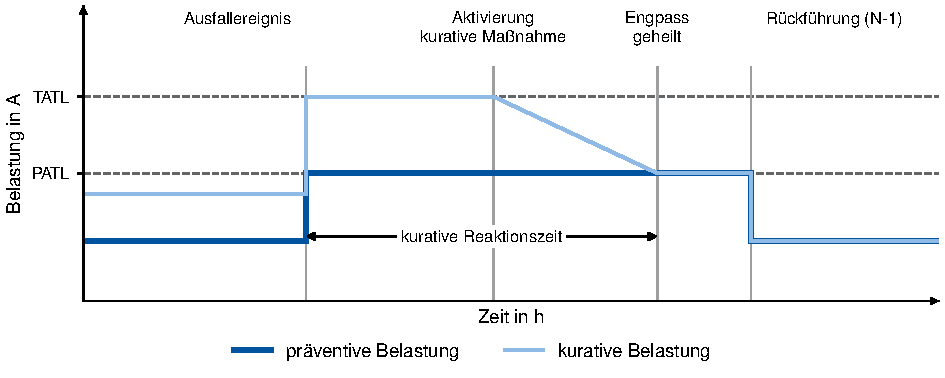
\includegraphics[width=\textwidth]{figures/chapter_2/preventiv_vs_curative_redispatch.pdf}
    \caption{Vergleich der zeitlichen Betriebsmittelbelastung bei präventiver und kurativer Systemführung im Fehlerfall.}
    \label{fig:preventiv_kurativ}
\end{figure}

% NEU GEFASST am 15.09.2026 nach dem Absatzplan im Sammelmodus.
% Befunde B47 bis B52, Q1, Q3, V5, V13. Marge als Vorgabe des Netzes, Hoehe statt Breite, Planungshorizont statt Reichweite mit Zeiten, Beleg sous fuer die Kostenwirkung entfallen, weil die Quelle nur die Marge definiert.
% Alte Fassung, nicht wieder aufnehmen:
%Kosten und Grenze dieses präventiven Vorgehens folgen aus drei Merkmalen.
%Erstens beruht die Robustheit auf einer Sicherheitsmarge, die die Vorauslastung so weit begrenzt, dass die Belastung auch nach einem Ausfall unterhalb der \ac{PATL} bleibt, und die den dafür erforderlichen Eingriff in die Fahrpläne verursacht.
%Die Breite dieser Marge wirkt damit unmittelbar auf Volumen und Kosten des Redispatch \cite{sous_comparison_2025}.
%Zweitens endet die Reichweite des Ansatzes mit der letzten Prognoserechnung, die vor dem Erfüllungszeitpunkt liegt.
%Fahrplanänderungen aus dem danach verbleibenden Handelsfenster sind in ihr nicht mehr enthalten, und auf die daraus entstehenden Netzzustände lässt sich präventiv nicht mehr reagieren.
%Drittens hängen die Kosten einer Maßnahme nicht allein vom Eingriffsvolumen ab, sondern von der Art der herangezogenen Anlagen, weil sich der finanzielle Ausgleich je nach Anlagenklasse unterschiedlich bemisst \cite{bundesministerium_der_justiz_energiewirtschaftsgesetz_2025, bundesnetzagentur_festlegung_2024}.
%Stehen für einen Engpass nur wenige geeignete Anlagen zur Verfügung, kann bereits ein moderates Eingriffsvolumen hohe Kosten verursachen.
%Der Kreis geeigneter Anlagen verkleinert sich dabei, denn der Kohle- und Kernenergieausstieg reduziert die verfügbare steuerbare konventionelle Kapazität, während die Opportunitätskosten und Revisionsaufwände der verbleibenden Anlagen steigen \cite{innosys_2030_gesamtverbund_innovationen_2021}.
%Volumen und Kosten des präventiven Engpassmanagements entwickeln sich daher nicht proportional zueinander.
% UEBERLEITUNG am 19.09.2026, zweite Umstellung: der Absatz steht jetzt hinter dem kurativen
% Teil und braucht nach Stilregel 3 einen Anschluss. Alte Fassung:
%Kosten und Grenze des präventiven Vorgehens folgen aus drei Merkmalen.
% AUFZAEHLUNG AUFGELOEST am 19.09.2026, Kommentar des Verfassers: "danach wuerde ich aber direkt ueberleiten dazu dass das ein kleiner kreis an anlagen ist, was dann auch wieder mit drittens zusammenhaengt, weswegen allgemein diese erstens zweitens drittens aufteilung keinen sinn ergibt". Der Absatz laeuft jetzt als Kette: Sicherheitsmarge, Redispatch, Kosten, Ende des Planungshorizonts, kleiner Kreis an Anlagen, Kostenwirkung der Anlagenart, Verlagerung in die Kurzfrist. Alte Fassung:
%Den Anlass für kurative Maßnahmen geben die Kosten und die Grenze des präventiven Vorgehens, die aus drei Merkmalen folgen.
Den Anlass für kurative Maßnahmen geben die Kosten und die Grenze des präventiven Vorgehens.
% R-14 am 18.09.2026, Kontrolle durch Fable, Entscheidung des Verfassers: Satz geteilt, Stilregel 17. Alte Fassung:
%Erstens beruht die Sicherheit auf einer Marge zwischen der Vorauslastung und dem \ac{PATL}, die nicht gewählt wird, sondern aus der ungünstigsten Ausfallvariante folgt, und das Freihalten dieser Marge ist der Eingriff in die Fahrpläne.
% UMSTELLUNG am 19.09.2026: der PATL wird erst im kurativen Teil eingefuehrt, hier steht deshalb
% die deutsche Bezeichnung aus dem Abkuerzungsverzeichnis. Alte Fassung:
%Erstens beruht die Sicherheit auf einer Marge zwischen der Vorauslastung und dem \ac{PATL}, die nicht gewählt wird, sondern aus der ungünstigsten Ausfallvariante folgt.
% PATL WIEDER ALS AKRONYM am 19.09.2026, zweite Umstellung: der PATL ist jetzt im Absatz davor
% definiert, die Umschreibung vom selben Tag ist damit gegenstandslos. Zurueckgenommene Fassung:
%Erstens beruht die Sicherheit auf einer Marge zwischen der Vorauslastung und der dauerhaft zulässigen Strombelastbarkeit, die nicht gewählt wird, sondern aus der ungünstigsten Ausfallvariante folgt.
% BEGRIFF PRAEVENTIVE SICHERHEITSMARGE am 19.09.2026, vierter Kommentar des Verfassers: "die
% praeventive sicherheitsmarge beschreibt es vielleicht besser, die mehr redispatch erfordert,
% welches dann mehr kosten erzeugt". Das Attribut praeventiv grenzt die Marge gegen den Abstand
% ab, den auch die kurative Systemfuehrung zum jeweils massgeblichen Grenzwert einhaelt. Die
% Wendung "die Sicherheit beruht auf einer Sicherheitsmarge" waere doppelt, deshalb steht jetzt
% der praeventive Ansatz als Subjekt, Stilregel 10. Alte Fassung:
%Erstens beruht die Sicherheit auf einer Marge zwischen der Vorauslastung und dem \ac{PATL}, die nicht gewählt wird, sondern aus der ungünstigsten Ausfallvariante folgt.
% Ordnungszahl entfallen, Aufloesung der Aufzaehlung. Alte Fassung:
%Erstens verlangt der präventive Ansatz eine Sicherheitsmarge zwischen der Vorauslastung und dem \ac{PATL}, die nicht gewählt wird, sondern aus der ungünstigsten Ausfallvariante folgt.
Der präventive Ansatz verlangt eine Sicherheitsmarge zwischen der Vorauslastung und dem \ac{PATL}, die nicht gewählt wird, sondern aus der ungünstigsten Ausfallvariante folgt.
% SAETZE VERBUNDEN am 19.09.2026, Kommentar des Verfassers: "das kann verbunden werden um nicht
% immer so viel marge zu schreiben". Das Wort Marge stand in drei aufeinanderfolgenden Saetzen,
% jetzt in zweien. Der verbundene Satz traegt zwei Hauptsaetze und keinen Nebensatz, Stilregel 17.
% Alte Fassung:
%Das Freihalten dieser Marge ist der Eingriff in die Fahrpläne.
%Die Höhe der Marge bestimmt damit Volumen und Kosten des präventiven Redispatch.
% KAUSALITAET BERICHTIGT am 19.09.2026, Kommentar des Verfassers: "da steht die kausalitaet nicht
% richtig, um die sicherheitsmarge zu gewaehrleisten muss in die fahrplaene eingegriffen werden".
% Die alte Fassung setzte das Freihalten der Marge mit dem Eingriff gleich. Jetzt ist die Marge das
% Ziel und der Eingriff das Mittel, und der UeNB steht als handelnder Akteur im Subjekt,
% Stilregel 10. Alte Fassung:
%Das Freihalten dieser Marge ist der Eingriff in die Fahrpläne, und ihre Höhe bestimmt Volumen und Kosten des präventiven Redispatch.
% KAUSALKETTE AUSGESCHRIEBEN am 19.09.2026, zweiter Kommentar des Verfassers: "der uenb haelt die
% marge frei unter anderem durch redispatch welches dann durch eingriffe in fahrplaene verguetet
% werden muss und kosten erzeugt". Die Kette lautet jetzt Marge, praeventiver Redispatch,
% Fahrplanaenderung, finanzieller Ausgleich, Kosten. Zwei Saetze, weil ein Satz mit zwei
% Hauptsaetzen keinen Nebensatz mehr traegt, Stilregel 17. Das Wort Marge steht weiter nur zweimal,
% weil der zweite Satz das Volumen der Fahrplanaenderungen aufgreift und nicht die Marge. Der
% finanzielle Ausgleich ist im dritten Merkmal desselben Absatzes belegt, Stilregel 15. Alte
% Fassung:
%Der \ac{ÜNB} hält diese Marge durch einen Eingriff in die Fahrpläne frei, und ihre Höhe bestimmt Volumen und Kosten des präventiven Redispatch.
% KOSTENURSACHE BERICHTIGT am 19.09.2026, dritter Kommentar des Verfassers: "generell ist nicht
% die marge die kosten erzeugt, da sie auch bei kurativ insofern eingehalten werden muss. der
% redispatch erzeugt die kosten". Die Marge ist eine Vorgabe des Netzes und keine Kostenquelle,
% denn auch die kurative Systemfuehrung haelt einen Abstand ein, naemlich zum TATL statt zum PATL.
% Kosten verursacht die Massnahme, mit welcher der UeNB die Marge freihaelt. Alte Fassung:
%Der \ac{ÜNB} hält diese Marge unter anderem durch präventiven Redispatch frei, und ihre Höhe bestimmt das Volumen der dafür nötigen Fahrplanänderungen.
%Die Fahrplanänderungen muss der \ac{ÜNB} finanziell ausgleichen, sodass mit dem Volumen die Kosten des präventiven Redispatch steigen.
% KETTE NACH DEM VERFASSER am 19.09.2026: groessere praeventive Sicherheitsmarge, mehr Redispatch,
% mehr Kosten. Die Verneinung der alten Fassung entfaellt, weil die Kette die Kostenursache beim
% Redispatch ohnehin benennt. Alte Fassung:
%Die Kosten verursacht nicht die Marge, sondern der präventive Redispatch, mit dem der \ac{ÜNB} sie freihält.
%Der \ac{ÜNB} gleicht jede angeordnete Fahrplanänderung finanziell aus, sodass die Kosten mit dem Volumen des Redispatch steigen.
Je größer diese präventive Sicherheitsmarge ausfällt, desto mehr präventiven Redispatch erfordert sie.
Für den angeordneten Redispatch leistet der \ac{ÜNB} einen finanziellen Ausgleich, sodass mit seinem Volumen auch die Kosten steigen.
% SATZLAENGE am 15.09.2026, Stilregel 17, alte Fassung als Kommentar:
%Zweitens reicht der Planungshorizont des Ansatzes, also der Zeitraum, den die Vorschaurechnungen abdecken, nur bis zur letzten Vorschaurechnung, nämlich der Vortagesrechnung und den untertägigen Rechnungen, die Abbildung~\ref{fig:markt_zeitschiene} auf der Zeitachse zeigt, während der Handel innerhalb einer Regelzone bis fünf Minuten vor Lieferung offen bleibt.
% BEZUG AUSGESCHRIEBEN am 19.09.2026, zweite Umstellung, Stilregel 5: der vorige Absatz handelt
% vom kurativen Ansatz, der Ansatz ohne Attribut waere hier nicht mehr eindeutig. Alte Fassung:
%Zweitens reicht der Planungshorizont des Ansatzes, also der Zeitraum, den die Vorschaurechnungen abdecken, nur bis zur letzten Vorschaurechnung.
% VIER SAETZE AUF DREI am 19.09.2026, Kommentar des Verfassers: "ich wuerde hier nicht verweisen
% sondern einfach schreiben auf abbildungen die viel spaeter kommen ... den satz wuerde ich einfach
% aendern zu einem kompakten satz". Der Verweis auf Abbildung 2.3 stand elf Seiten vor der
% Abbildung und ist gestrichen, ebenso der Verweis auf Abschnitt 2.2.2 und die Aufzaehlung der
% Vorschaurechnungen. Die Begruendung ueber den offenen Handel bleibt ohne Verweis erhalten, weil
% der Absatz sonst unbelegt behauptet, dass es Fahrplanaenderungen nach der letzten
% Vorschaurechnung gibt. Der Planungshorizont wird weiter erklaert, CLAUDE.md Abschnitt 5.
% Gestrichene Saetze:
%Die letzte Vorschaurechnung ist die Vortagesrechnung oder eine der untertägigen Rechnungen, die Abbildung~\ref{fig:markt_zeitschiene} auf der Zeitachse zeigt.
%Der Handel bleibt dagegen bis kurz vor Lieferung offen, wie in Abschnitt~\ref{sec:market_horizons} dargestellt.
%Fahrplanänderungen aus diesem Zeitraum enthält keine Vorschaurechnung mehr, sodass der \ac{ÜNB} die daraus entstehenden Netzzustände nur noch mit den Mitteln beheben kann, die ohne Vorlauf verfügbar sind.
% Alte Fassung des Eingangssatzes:
%Zweitens reicht der Planungshorizont des präventiven Ansatzes, also der Zeitraum, den die Vorschaurechnungen abdecken, nur bis zur letzten Vorschaurechnung.
Die Vorschaurechnungen decken den Planungshorizont des präventiven Ansatzes ab, der Handel bleibt dagegen bis kurz vor Lieferung offen.
Netzzustände aus Fahrplanänderungen nach der letzten Vorschaurechnung kann der \ac{ÜNB} nur noch mit Mitteln ohne Vorlauf beheben.
Ohne Vorlauf kommt nur ein kleiner Kreis von Anlagen in Betracht.
%Die letzte Vorschaurechnung ist die Vortagesrechnung oder eine der untertägigen Rechnungen, die Abbildung~\ref{fig:markt_zeitschiene} auf der Zeitachse zeigt.
% R-14 am 18.09.2026, Kontrolle durch Fable, Entscheidung des Verfassers: die Handelsschlusszeiten stehen in 2.2.2, hier genuegt der Verweis. Alte Fassung:
%Der Handel innerhalb einer Regelzone bleibt dagegen bis fünf Minuten vor Lieferung offen.
%Der Handel bleibt dagegen bis kurz vor Lieferung offen, wie in Abschnitt~\ref{sec:market_horizons} dargestellt.
%Fahrplanänderungen aus diesem Zeitraum enthält keine Vorschaurechnung mehr, sodass der \ac{ÜNB} die daraus entstehenden Netzzustände nur noch mit den Mitteln beheben kann, die ohne Vorlauf verfügbar sind.
% SATZLAENGE am 15.09.2026, Stilregel 17, alte Fassung als Kommentar:
%Drittens hängen die Kosten einer Maßnahme nicht allein vom Eingriffsvolumen ab, sondern von der Art der herangezogenen Anlagen, weil sich der finanzielle Ausgleich je nach Anlagenklasse unterschiedlich bemisst \cite{bundesministerium_der_justiz_energiewirtschaftsgesetz_2025, bundesnetzagentur_festlegung_2024}, sodass bereits ein moderates Eingriffsvolumen hohe Kosten verursachen kann, wenn nur wenige geeignete Anlagen zur Verfügung stehen.
% ABSAETZE VERBUNDEN am 19.09.2026, Vorgabe des Verfassers: "mir werden hier viel zu viel absaetze gemacht ... ein absatz sollte eigentlich mal mindestens eine halbe seite lang sein". Die Leerzeile stand hier bis zum 19.09.2026. Erstens, zweitens und drittens gehoeren in einen Absatz, eine Aufzaehlung darf keine Absatzgrenze haben.
% NEUER ABSATZ 16.09.2026, C2.2.
% Ordnungszahl durch den Anschluss deshalb ersetzt, Aufloesung der Aufzaehlung. Alte Fassung:
%Drittens hängen die Kosten einer Maßnahme nicht allein vom Eingriffsvolumen ab, sondern von der Art der herangezogenen Anlagen, weil sich der finanzielle Ausgleich je nach Anlagenklasse unterschiedlich bemisst \cite{bundesministerium_der_justiz_energiewirtschaftsgesetz_2025, bundesnetzagentur_festlegung_2024}.
Die Kosten einer Maßnahme hängen deshalb nicht allein vom Eingriffsvolumen ab, sondern von der Art der herangezogenen Anlagen, weil sich der finanzielle Ausgleich je nach Anlagenklasse unterschiedlich bemisst \cite{bundesministerium_der_justiz_energiewirtschaftsgesetz_2025, bundesnetzagentur_festlegung_2024}.
Stehen nur wenige geeignete Anlagen zur Verfügung, kann bereits ein moderates Eingriffsvolumen hohe Kosten verursachen.
Der Kreis geeigneter Anlagen verkleinert sich zugleich, denn der Kohle- und Kernenergieausstieg reduziert die steuerbare konventionelle Kapazität, während die Opportunitätskosten und Revisionsaufwände der verbleibenden Anlagen steigen \cite{innosys_2030_gesamtverbund_innovationen_2021}.
% ANS ABSATZENDE VERSCHOBEN am 19.09.2026: der Satz zieht die Folge aus der ganzen Kette und
% steht deshalb am Schluss und nicht mehr in der Mitte. Verschobener Satz:
%Volumen und Kosten des präventiven Engpassmanagements entwickeln sich daher nicht proportional zueinander.
% ABSAETZE VERBUNDEN am 19.09.2026, Vorgabe des Verfassers: "mir werden hier viel zu viel absaetze gemacht ... ein absatz sollte eigentlich mal mindestens eine halbe seite lang sein". Die Leerzeile stand hier bis zum 19.09.2026. Die Verstaerkung durch die kurzfristigen Maerkte gehoert zu Kosten und Grenze des praeventiven Vorgehens.
% ABSATZ VERBUNDEN 16.09.2026, C2.2.
% NEU GEFASST am 15.09.2026 nach dem Absatzplan im Sammelmodus.
% Befunde B53, G12, Q2, V5. Fuenf Saetze auf drei, Beleg mahgoub steht in Kapitel 1.
% Alte Fassung, nicht wieder aufnehmen:
%Die begrenzte Reichweite und die Abhängigkeit der Kosten von der Anlagenart verstärken sich gegenseitig, weil sich die Fahrplanbildung zunehmend in die kurzfristigen Märkte verlagert.
%Mit den Intraday-Auktionen und dem kontinuierlichen Intraday-Handel ist ein wachsender Teil der Fahrplanbildung in die Stunden vor Lieferbeginn gerückt \cite{mahgoub_wie_2025}, und die Umstellung der Auktion des \ac{DA} auf Viertelstundenprodukte hat die Volumenverteilung zwischen den Handelszeitpunkten zusätzlich verändert \cite{ffe_saegezahn_2026}.
%Je später sich der maßgebliche Netzzustand einstellt, desto später ist auch der erforderliche Eingriff zu bestimmen.
%Mit der verbleibenden Vorlaufzeit sinkt jedoch die Zahl der Anlagen, die die geforderte Leistungsänderung noch erbringen können, weil ein Teil der in Betracht kommenden Technologien Vorlaufzeiten von mehreren Stunden aufweist.
%Ein kleinerer Kreis geeigneter Anlagen schlägt sich unmittelbar in den Kosten nieder.
% R-15 am 18.09.2026, Kontrolle durch Fable, Entscheidung des Verfassers: Satz geteilt, Stilregel 17. Alte Fassung:
%Der begrenzte Planungshorizont und die Abhängigkeit der Kosten von der Anlagenart verstärken sich gegenseitig, weil sich die Fahrplanbildung zunehmend in die kurzfristigen Märkte verlagert: Mit den Intraday-Auktionen und dem kontinuierlichen Intraday-Handel ist ein wachsender Teil der Fahrplanbildung in die Stunden vor Lieferbeginn gerückt, und die Umstellung der Auktion des \ac{DA} auf Viertelstundenprodukte hat die Volumenverteilung zwischen den Handelszeitpunkten zusätzlich verändert \cite{ffe_saegezahn_2026}.
% GEKUERZT am 19.09.2026: die beiden Ursachen sind im Absatz jetzt der Reihe nach entwickelt und
% muessen nicht wiederholt werden. Alte Fassung:
%Der begrenzte Planungshorizont und die Abhängigkeit der Kosten von der Anlagenart verstärken sich gegenseitig, weil sich die Fahrplanbildung zunehmend in die kurzfristigen Märkte verlagert.
Beide Ursachen verstärken sich, weil sich die Fahrplanbildung zunehmend in die kurzfristigen Märkte verlagert.
% TEILSATZ GESTRICHEN am 19.09.2026, Kommentar des Verfassers: "da bin ich mir noch nicht sicher
% ob das einen einfluss hat. eher doch auf die id auktionen da diese ja dann viertelstundenprodukte
% gefuehrt haben. ich glaube diese info wuerde ich erst diskutieren in kapitel 5". Der Beleg
% ffe_saegezahn_2026 traegt allein den gestrichenen Teilsatz, er steht weiter in 2.2.2, 2.3.5, 3.1
% und als Punkt in chapter_5.tex. Der verbleibende Satz traegt jetzt mahgoub_wie_2025, den Beleg
% der Fassung vom 15.09.2026 fuer genau diese Aussage. Alte Fassung:
%Mit den Intraday-Auktionen und dem kontinuierlichen Intraday-Handel ist ein wachsender Teil der Fahrplanbildung in die Stunden vor Lieferbeginn gerückt, und die Umstellung der Auktion des \ac{DA} auf Viertelstundenprodukte hat die Volumenverteilung zwischen den Handelszeitpunkten zusätzlich verändert \cite{ffe_saegezahn_2026}.
Mit den Intraday-Auktionen und dem kontinuierlichen Intraday-Handel ist ein wachsender Teil der Fahrplanbildung in die Stunden vor Lieferbeginn gerückt \cite{mahgoub_wie_2025}.
% SATZLAENGE am 15.09.2026, Stilregel 17, alte Fassung als Kommentar:
%Je später sich der maßgebliche Netzzustand einstellt, desto später ist der erforderliche Eingriff zu bestimmen, und mit der verbleibenden Vorlaufzeit sinkt die Zahl der Anlagen, die die geforderte Leistungsänderung noch erbringen können, weil ein Teil der Technologien Vorlaufzeiten von mehreren Stunden aufweist.
% ZWEI SAETZE AUF EINEN am 19.09.2026: der spaetere Eingriffszeitpunkt und der kleinere Kreis an
% Anlagen sind dieselbe Aussage, die der Absatz weiter oben schon einfuehrt. Danach folgt der vom
% Absatzende hierher gezogene Schlusssatz. Gestrichene Saetze:
%Je später sich der maßgebliche Netzzustand einstellt, desto später ist der erforderliche Eingriff zu bestimmen.
%Mit der verbleibenden Vorlaufzeit sinkt die Zahl der Anlagen, die die geforderte Leistungsänderung noch erbringen können.
%Je später sich der maßgebliche Netzzustand einstellt, desto später ist der erforderliche Eingriff zu bestimmen.
Der maßgebliche Netzzustand steht deshalb immer später fest, sodass noch weniger Anlagen die geforderte Leistungsänderung erbringen können.
Volumen und Kosten des präventiven Engpassmanagements entwickeln sich daher nicht proportional zueinander.
%Mit der verbleibenden Vorlaufzeit sinkt die Zahl der Anlagen, die die geforderte Leistungsänderung noch erbringen können.
% ERGAENZT am 19.09.2026, dritter Kommentar des Verfassers: "diese kosten werden durch verlagerung
% in die kurzfrist teurer". Der Absatz endete bisher bei der sinkenden Zahl der Anlagen und zog die
% Folge fuer die Kosten nicht, Stilregel 4. Eigenstaendige Ableitung aus den beiden Saetzen davor
% und aus dem dritten Merkmal desselben Absatzes, wonach die Kosten von der Art der herangezogenen
% Anlagen abhaengen.
% WIEDER GESTRICHEN am 19.09.2026, Kommentar des Verfassers: "das beschreiben wir schon durch die
% kurzfristigen eingriffe". Der Satz war am selben Tag ergaenzt worden und sagt nichts, was die
% Saetze zur Verlagerung in die kurzfristigen Maerkte nicht schon tragen. Nicht wieder aufnehmen:
%Der präventive Redispatch wird durch die Verlagerung in die Kurzfrist teurer, auch wenn sein Volumen gleich bleibt.
% DURCHSICHT 16.09.2026, C1. Alte Fassung:
%Ein Teil der Technologien weist Vorlaufzeiten von mehreren Stunden auf.
% R-15 am 18.09.2026, Kontrolle durch Fable, Entscheidung des Verfassers: gestrichen, die Aussage traegt keine Quelle. Gestrichener Satz: Alte Fassung:
%Ein Teil der Technologien weist nämlich Vorlaufzeiten von mehreren Stunden auf.
% S-16 am 18.09.2026, Kontrolle durch Fable, Entscheidung des Verfassers: gestrichen, die Aussage traegt Satz 2 desselben Absatzes. Gestrichener Satz: Alte Fassung:
%Ein kleinerer Kreis geeigneter Anlagen schlägt sich unmittelbar in den Kosten nieder.

% NEU GEFASST am 15.09.2026 nach dem Absatzplan im Sammelmodus.
% Befunde B54 bis B61, G13, G14, V5, V13. Auspraegungen beim Namen genannt, kurativer Redispatch wird ebenfalls vorgeplant, Behauptung zur Abdeckung spaeter Zustaende zurueckgenommen, Beleg fuer die Jahressimulation, Vorverweise gestrichen, zwei Absaetze.
% Alte Fassung, nicht wieder aufnehmen:
%Die kurative Systemführung setzt an der Sicherheitsmarge und an der begrenzten Reichweite an und tritt dabei in zwei Ausprägungen auf.
%Die kurative Höherauslastung begreift die thermische Reserve zwischen \ac{PATL} und \ac{TATL} als nutzbares Betriebsfenster und erlaubt eine bewusst höhere Vorauslastung im Normalbetrieb, wodurch der präventive Eingriffsbedarf sinkt.
%Der kurative Redispatch verzichtet auf eine solche Vorplanung und behebt eine Grenzwertverletzung, die sich erst nach der letzten Prognoserechnung eingestellt hat, innerhalb des zulässigen Überlastintervalls.
%Er ist damit die Antwort auf die begrenzte Reichweite, weil er Netzzustände abdeckt, für die sich präventiv keine Maßnahme mehr disponieren lässt.
%Beiden Ausprägungen ist gemeinsam, dass die Maßnahme erst nach dem Fehlereintritt wirkt und deshalb keinen vorherigen Eingriff in den Fahrplan erfordert.
%Darin liegt der Vorteil gegenüber dem präventiven Ansatz, denn dieser greift unabhängig davon in den Fahrplan ein, ob die Ausfallvariante überhaupt eintritt, während die kurative Maßnahme lediglich vorgehalten und allein im Fehlerfall abgerufen wird.
%Für den Anlagenbetreiber entfällt der Aufwand damit allerdings nicht, weil er das Stellpotenzial über die gesamte Bindungsdauer bereithalten muss.
%Jahressimulationen belegen für den kurativen Betrieb ein Einsparpotenzial gegenüber dem rein präventiven Ansatz.
%Wie groß dieses Potenzial ausfällt, hängt dabei stark davon ab, welche Anlagen kurativ einsetzbar sind, denn auf einem synthetischen Netzmodell mit Zieljahr 2037 sinken die Kosten des Engpassmanagements auf rund 42\,\% des rein präventiven Betriebs, solange allein Phasenschieber und \ac{HGÜ} zur Verfügung stehen, und auf rund 2\,\%, sobald zusätzlich die Abregelung erneuerbarer Erzeugung sowie \ac{PSKW} und \ac{BESS} einbezogen werden \cite{sous_comparison_2025}.
%Der Effizienzgewinn geht mit erhöhten Anforderungen an Automatisierungsgrad und Sicherheit einher, die Abschnitt \ref{sec:curative_functionality} anhand der Prozesskette und Abschnitt \ref{sec:challenges} anhand der offenen Umsetzungsfragen ausführen.
%Zugleich ändert sich die Art der entstehenden Kosten, da an die Stelle der Erzeugungsauslagen einer durchgeführten Maßnahme die Vorhaltekosten einer bereitgestellten Reaktionsfähigkeit treten.
%Für diese Kostenart kennt die Vergütungssystematik des Engpassmanagements keine Bemessungsgrundlage, was Abschnitt \ref{sec:redispatch_compensation} darlegt und Abschnitt \ref{sec:interim_conclusion} zusammenführt.
% BEGRIFF NACHGEZOGEN am 19.09.2026, Stilregel 14: die Marge heisst seit dem vierten Kommentar des
% Verfassers praeventive Sicherheitsmarge. Alte Fassung:
%Die kurative Systemführung setzt an der Marge und am Planungshorizont an und tritt in zwei Ausprägungen auf, nämlich der kurativen Höherauslastung und dem kurativen Redispatch.
Die kurative Systemführung setzt an der präventiven Sicherheitsmarge und am Planungshorizont an und tritt in zwei Ausprägungen auf, nämlich der kurativen Höherauslastung und dem kurativen Redispatch.
Die kurative Höherauslastung begreift die thermische Reserve zwischen \ac{PATL} und \ac{TATL} als nutzbares Betriebsfenster und erlaubt eine höhere Vorauslastung im Normalbetrieb, wodurch der präventive Eingriffsbedarf sinkt.
% SATZLAENGE am 15.09.2026, Stilregel 17, alte Fassung als Kommentar:
%Der kurative Redispatch wird ebenfalls vorab eingeplant und scharfgeschaltet, der Unterschied zur präventiven Planung liegt im angesetzten Grenzwert, denn die Maßnahme wird erst ausgeführt, nachdem der Fehler eingetreten und die Überlastung tatsächlich vorhanden ist, und behebt die Überlastung innerhalb der zulässigen Überlastdauer.
% DURCHSICHT 16.09.2026, C1. Alte Fassung:
%Der kurative Redispatch wird ebenfalls vorab eingeplant und scharfgeschaltet.
% NEU GEFASST am 19.09.2026, Kommentar des Verfassers: "kurativer redispatch koennte man einfach
% die kurative massnahme nicht als hoeherauslastungpotential begreifen sondern als vorgeplante
% zusaetzliche sicherung der n-1 grenzen". Der Satz sagte bisher nur, dass auch der kurative
% Redispatch vorab eingeplant wird, und nannte den Zweck nicht. Jetzt steht die Abgrenzung zur
% Hoeherauslastung im Satz. Alte Fassung:
%Auch der kurative Redispatch wird vorab eingeplant und scharfgeschaltet.
Der kurative Redispatch nutzt dieselbe Reserve dagegen nicht für eine höhere Vorauslastung, sondern sichert mit ihr das \mbox{(N-1)-Kriterium} durch eine vorab eingeplante Maßnahme ab.
% ZWECK ERGAENZT am 19.09.2026, Kommentar des Verfassers: "ohne den fahrplan zu aendern kannst du
% streichen. es wird ja dann dafuer eingesetzt, dass wenn kurzfristig engpassmanagement gemacht
% werden muss die kurative massnahme nur die systemsicherheit gewaehrleistet statt noch teurer
% kurzfristige massnahmen zu ergreifen". Der Absatz schliesst damit an den Absatz davor an, der
% den kleinen Kreis kurzfristig verfuegbarer Anlagen und seine Kostenwirkung entwickelt. Die
% Aussage des ersten Satzes, die kurative Systemfuehrung setze auch am Planungshorizont an, ist
% damit wieder getragen, und zwar als Kostenargument und nicht als Behauptung ueber die Abdeckung
% spaet entstehender Netzzustaende, die am 15.09.2026 zurueckgenommen worden ist. Alte Fassung:
%Der \ac{ÜNB} plant die Maßnahme für eine Ausfallvariante ein und schaltet sie scharf, ohne den Fahrplan vorher zu ändern.
Der \ac{ÜNB} plant die Maßnahme für eine Ausfallvariante ein und schaltet sie scharf.
Wird der Eingriff erst kurzfristig erforderlich, wahrt die kurative Maßnahme die Systemsicherheit.
Ein kurzfristiger präventiver Redispatch mit dem kleinen Kreis verfügbarer Anlagen wird dann nicht nötig.
% DURCHSICHT 16.09.2026, C1, These und Erklaerung. Alte Fassung:
%Der Unterschied zur präventiven Planung liegt im angesetzten Grenzwert: Die Maßnahme wird erst ausgeführt, nachdem der Fehler eingetreten und die Überlastung tatsächlich vorhanden ist.
Der Unterschied zur präventiven Planung liegt im angesetzten Grenzwert und im Zeitpunkt: Die Maßnahme wird erst ausgeführt, nachdem der Fehler eingetreten und die Überlastung tatsächlich vorhanden ist, und behebt sie innerhalb der zulässigen Überlastdauer.
% DURCHSICHT 16.09.2026, C1, im Vorsatz aufgegangen: Die Maßnahme behebt die Überlastung dann innerhalb der zulässigen Überlastdauer.
% GESTRICHEN am 19.09.2026, Kommentar des Verfassers: "das verstehe ich nicht". Der Satz war die
% abgeschwaechte Fassung der am 15.09.2026 zurueckgenommenen Behauptung, der kurative Redispatch
% decke Netzzustaende ab, fuer die sich praeventiv keine Massnahme mehr disponieren laesst. Uebrig
% blieb eine Aussage ohne Inhalt, naemlich dass die Abdeckung von der Einplanung abhaengt. Die
% Einplanung fuer eine Ausfallvariante steht jetzt im Satz zum kurativen Redispatch selbst.
% Gestrichener Satz, nicht wieder aufnehmen:
%Weil auch der kurative Redispatch vorab eingeplant wird, hängt es von der Einplanung für die betroffene Ausfallvariante ab, ob eine kurative Maßnahme einen Netzzustand abdeckt, der erst nach der letzten Vorschaurechnung entsteht.
% R-17 am 18.09.2026, Kontrolle durch Fable: von Absatz 11 bleibt allein dieser Satz, er haengt jetzt an Absatz 10.
% BEZUG AUSGESCHRIEBEN am 19.09.2026: das Wort damit verwies auf den gestrichenen Satz davor und
% ist durch den gemeinten Fall ersetzt, naemlich die Vorhaltung ohne Abruf, Stilregel 5. Alte
% Fassung:
%Für den Anlagenbetreiber entfällt der Aufwand damit nicht, weil er das Stellpotenzial über die gesamte Bindungsdauer bereithalten muss.
% BEGRIFF am 20.09.2026, Vorgabe des Verfassers: EIV statt Anlagenbetreiber, weil hier die Rolle gemeint ist,
% die den Fahrplan bestimmt und die Zusage gibt. Alte Fassung:
%Auch ohne Abruf entsteht dem Anlagenbetreiber Aufwand, weil er das Stellpotenzial über die gesamte Bindungsdauer bereithalten muss.
Auch ohne Abruf entsteht dem \ac{EIV} Aufwand, weil er das Stellpotenzial über die gesamte Bindungsdauer bereithalten muss.

% S-01 am 18.09.2026, Kontrolle durch Fable, Entscheidung des Verfassers: gestrichen, die Aussage traegt Absatz 10 Satz 4 und 1.1 Absatz 11. Gestrichener Satz: Alte Fassung:
%Der kurativen Höherauslastung und dem kurativen Redispatch ist gemeinsam, dass die Maßnahme erst nach dem Fehlereintritt wirkt und deshalb keinen vorherigen Eingriff in den Fahrplan erfordert.
% SATZLAENGE am 15.09.2026, Stilregel 17, alte Fassung als Kommentar:
%Der Vorteil gegenüber dem präventiven Ansatz liegt darin, dass der präventive Ansatz unabhängig davon in den Fahrplan eingreift, ob die Ausfallvariante eintritt, während die kurative Maßnahme lediglich vorgehalten und allein im Fehlerfall abgerufen wird.
% S-01 am 18.09.2026, Kontrolle durch Fable, Entscheidung des Verfassers: gestrichen, die Aussage traegt 1.1 Absatz 11. Gestrichener Satz: Alte Fassung:
%Der Vorteil gegenüber dem präventiven Ansatz liegt darin, dass der präventive Ansatz unabhängig vom Eintritt der Ausfallvariante in den Fahrplan eingreift.
% S-01 am 18.09.2026, Kontrolle durch Fable, Entscheidung des Verfassers: gestrichen, die Aussage traegt Absatz 10 Satz 4. Gestrichener Satz: Alte Fassung:
%Die kurative Maßnahme wird dagegen lediglich vorgehalten und allein im Fehlerfall abgerufen.
% SATZLAENGE am 15.09.2026, Stilregel 17, alte Fassung als Kommentar:
%Jahressimulationen belegen für den kurativen Betrieb ein Einsparpotenzial gegenüber dem rein präventiven Ansatz, dessen Höhe davon abhängt, welche Anlagen kurativ einsetzbar sind: Auf einem synthetischen Netzmodell mit Zieljahr 2037 sinken die Kosten des Engpassmanagements auf rund 42\,\% des rein präventiven Betriebs, solange allein Phasenschieber und \ac{HGÜ} zur Verfügung stehen, und auf rund 2\,\%, sobald zusätzlich die Abregelung erneuerbarer Erzeugung sowie \ac{PSKW} und \ac{BESS} einbezogen werden \cite{sous_comparison_2025}.

% NEUER ABSATZ 16.09.2026, C2.3.
Jahressimulationen belegen für den kurativen Betrieb ein Einsparpotenzial gegenüber dem rein präventiven Ansatz \cite{sous_comparison_2025}.
% RANDBEDINGUNG ERGAENZT und ZAHL BERICHTIGT am 19.09.2026, Kommentar des Verfassers:
% "synthetisches netzmodell mit vereinfachten kostenannahmen". Nachgelesen in der Quelle, Abschnitt
% zu den Kostenannahmen: "The costs assumed for preventive CM represent the order for deployment of
% RAs (grid-related before market-related) and should roughly reflect the cost distribution of
% preventive CM", mit Kostenparametern wie HGUE 1 Euro je MW, PST 5 Euro je Grad, Speicher 80 und
% 237 Euro je MW, Kraftwerke 54 bis 160 Euro je MW, Erneuerbare 2170 Euro je MW und
% grenzueberschreitender Redispatch 10000 Euro je MW. Die Annahmen bilden also eine Reihenfolge ab
% und keine Marktpreise, die Randbedingung ist damit belegt.
% ZAHL BERICHTIGT: Tabelle 2 der Quelle weist fuer die Variante Reference Curative die Werte
% 42,07 Prozent (Cons.) und 1,57 Prozent (Amb.) des rein praeventiven Betriebs aus. Die bisherige
% Angabe "rund 2 Prozent" trifft keinen Wert der Tabelle, 2,45 Prozent gehoert zur Variante
% Redundanzkonzept 3. Richtig ist rund 1,6 Prozent. Alte Fassung:
%Die Höhe des Potenzials hängt davon ab, welche Anlagen kurativ einsetzbar sind: Auf einem synthetischen Netzmodell mit Zieljahr 2037 sinken die Kosten des Engpassmanagements auf rund 42\,\% des rein präventiven Betriebs, solange allein Phasenschieber und \ac{HGÜ} zur Verfügung stehen.
%Werden zusätzlich die Abregelung erneuerbarer Erzeugung sowie \ac{PSKW} und \ac{BESS} einbezogen, sinken die Kosten auf rund 2\,\%.
Die Höhe des Potenzials hängt davon ab, welche Anlagen kurativ einsetzbar sind: Auf einem synthetischen Netzmodell mit Zieljahr 2037 und vereinfachten Kostenannahmen sinken die Kosten des Engpassmanagements auf rund 42\,\% des rein präventiven Betriebs, solange allein Phasenschieber und \ac{HGÜ} zur Verfügung stehen.
Werden zusätzlich die Abregelung erneuerbarer Erzeugung sowie \ac{PSKW} und \ac{BESS} einbezogen, sinken die Kosten auf rund 1{,}6\,\%.
% ERGAENZT am 19.09.2026, Stilregel 8: die Quelle schliesst die Uebertragung ausdruecklich aus,
% "not all statements that apply to the grid model and scenario used in this work can be
% transferred to a real-scale scenario (e.g., the German transmission grid)".
Die Verfasser der Studie übertragen ihre Ergebnisse ausdrücklich nicht auf ein reales Netz wie das deutsche Übertragungsnetz.
% ERGAENZT am 19.09.2026, Kommentar des Verfassers: "danach kommen wir ja dazu was kurativ kostet
% und wenn kurativ guenstig ist kann man es sowohl fuer hoeherauslastung als auch fuer kurzfristige
% absicherung der systemgrenzen einsetzen". Der Satz zieht die Folge aus den beiden Auspraegungen
% und den Kosten und leitet zu der Frage ueber, fuer welche Kostenart die Verguetungssystematik
% keine Regel kennt.
% NEU GEFASST am 19.09.2026, Kommentar des Verfassers: "ich wuerde eher ueberleiten dass diese
% wirksamkeit unweigerlich mit den kosten zusammenhaengt und deswegen eine detailliertere
% untersuchung moeglicher kosten auch einen besseren ueberblick fuer eine erneute bewertung geben
% wuerde". Der Satz behauptete bisher, die Vorhaltung lasse sich bei guenstigem Preis fuer beide
% Auspraegungen einsetzen; das war eine Setzung ohne Beleg. Jetzt steht die Abhaengigkeit des
% Potenzials von den Kosten, und der Schluss des Absatzes benennt den Erkenntnisbedarf. Alte
% Fassung, nicht wieder aufnehmen:
%Bleibt die Vorhaltung günstig, lässt sie sich für beide Ausprägungen einsetzen, nämlich für die Höherauslastung und für die kurzfristige Absicherung der Systemgrenzen.
Die Wirksamkeit der kurativen Systemführung hängt an den Kosten der Vorhaltung.
% ANSCHLUSS ANGEPASST am 19.09.2026: das Wort zugleich bezog sich auf den ersetzten Satz. Alte
% Fassung:
%Zugleich ändert sich die Art der entstehenden Kosten, da an die Stelle der Erzeugungsauslagen einer durchgeführten Maßnahme die Vorhaltekosten einer bereitgestellten Reaktionsfähigkeit treten.
Die Art der entstehenden Kosten ändert sich dabei, da an die Stelle der Erzeugungsauslagen einer durchgeführten Maßnahme die Vorhaltekosten einer bereitgestellten Reaktionsfähigkeit treten.
% GESTRICHEN am 19.09.2026, Kommentar des Verfassers: "pruefe diese aussage auf dopplung.
% eigentlich sollte sie nicht in diesen absatz gehoeren oder?" Eigenstaendige Pruefung des ganzen
% Kapitels: die Aussage, dass die Vorhaltung keine Verguetungsregel kennt, steht ausser hier an
% fuenf weiteren Stellen, naemlich in 2.1.5 dreimal (Gegenstand ist der durchgefuehrte Eingriff und
% nicht die vorgehaltene Reaktionsfaehigkeit; keine Verguetung der Vorhaltung fuer eine am Markt
% bleibende Anlage; weil das EnWG die Vorhaltung nicht verguetet), in 2.3.5 (die Bemessung bietet
% keinen Anhalt) und in 2.4 (fuer eine kurative Bindung kennt das Engpassmanagement keinen
% Bemessungsgegenstand). Die Kette ist gewollt und muendet in 2.4. Diese Stelle war die
% Vorwegnahme: sie behauptet in 2.1.1, was erst 2.1.5 mit Paragraf 13a Abs. 2, Abs. 4 und
% Paragraf 13c traegt. CLAUDE.md und WORKFLOW.md benennen genau diesen Fehlertyp. Der Absatz
% behaelt die Aussage ueber die Art der Kosten und den Erkenntnisbedarf und ueberlaesst die
% rechtliche Folgerung dem rechtlichen Rahmen. Gestrichener Satz, nicht wieder aufnehmen:
%Für diese Kostenart kennt der finanzielle Ausgleich nach §\,13a \ac{EnWG} keine Regel, nach der sie zu vergüten wäre, denn er knüpft an die durchgeführte Anpassung an \cite{bundesministerium_der_justiz_energiewirtschaftsgesetz_2025}.
% ERGAENZT am 19.09.2026, Kommentar des Verfassers, Schluss der Ueberleitung: der Erkenntnisbedarf
% steht am Absatzende. Kein struktureller Vorverweis, Stilregel 15.
Eine nähere Untersuchung dieser Kosten gäbe deshalb einen besseren Überblick für eine erneute Bewertung des Einsparpotenzials.
% ABSAETZE VERBUNDEN am 19.09.2026, Vorgabe des Verfassers: "mir werden hier viel zu viel absaetze gemacht ... ein absatz sollte eigentlich mal mindestens eine halbe seite lang sein". Die Leerzeile stand hier bis zum 19.09.2026. Das Einsparpotenzial und seine Einordnung durch InnoSys 2030 tragen eine Kernaussage.
% NEU GEFASST am 15.09.2026 nach dem Absatzplan im Sammelmodus.
% Befunde B62, G15. Spaet auf die letzte Vorschaurechnung bezogen, Verweis auf Kapitel 4 gestrichen, Wendung die vorliegende Arbeit nach Stilregel 5 ersetzt.
% Alte Fassung, nicht wieder aufnehmen:
%Beide Ausprägungen greifen auf dieselbe thermische Reserve zu, denn was die Betriebsplanung vorab belegt, steht für spät entstehende Netzzustände nicht mehr zur Verfügung.
%Die Literatur fasst die kurative Systemführung überwiegend als Höherauslastung und misst ihren Nutzen an der Senkung des präventiven Eingriffsbedarfs \cite{innosys_2030_gesamtverbund_innovationen_2021}.
%Für den Akteur, der die Reaktionsfähigkeit bereitstellt, ist der Vorgang in beiden Fällen derselbe, denn er hält Leistung und Ladezustandsbereich für einen ungewissen Abruf frei.
%Die vorliegende Arbeit betrachtet deshalb die Vorhaltung als solche und behandelt die Bindungsdauer als Produktmerkmal, dessen Wirkung Abschnitt \ref{sec:sensitivities} untersucht.
% SATZLAENGE am 15.09.2026, Stilregel 17, alte Fassung als Kommentar:
%Beide Ausprägungen greifen auf dieselbe thermische Reserve zu, denn die Höherauslastung belegt die Reserve in der Betriebsplanung vorab, und was dort belegt ist, steht dem kurativen Redispatch für Netzzustände, die erst nach der letzten Vorschaurechnung entstehen, nicht mehr zur Verfügung.
% VERSCHOBEN 16.09.2026, C1, Reihenfolge in Absatz 12: Beide Ausprägungen greifen auf dieselbe thermische Reserve zu, denn die Höherauslastung belegt die Reserve in der Betriebsplanung vorab.
% VERSCHOBEN 16.09.2026, C1, Reihenfolge in Absatz 12: Was dort belegt ist, steht dem kurativen Redispatch für Netzzustände nach der letzten Vorschaurechnung nicht mehr zur Verfügung.
% R-18 am 18.09.2026, Kontrolle durch Fable, Entscheidung des Verfassers: eine Quelle traegt die Aussage, also wird sie benannt. Alte Fassung:
%Die Literatur fasst die kurative Systemführung überwiegend als Höherauslastung und misst ihren Nutzen an der Senkung des präventiven Eingriffsbedarfs \cite{innosys_2030_gesamtverbund_innovationen_2021}.
% ERGAENZT am 19.09.2026, Vorgabe des Verfassers: hier steht, was InnoSys 2030 erarbeitet hat. Alte Fassung:
%InnoSys~2030 fasst die kurative Systemführung überwiegend als Höherauslastung und misst ihren Nutzen an der Senkung des präventiven Eingriffsbedarfs \cite{innosys_2030_gesamtverbund_innovationen_2021}.
InnoSys~2030 hat den Maßnahmenraum kurativer Eingriffe und die Anforderungen an ihre Umsetzungszeiten systematisiert und fasst die kurative Systemführung dabei überwiegend als Höherauslastung, deren Nutzen das Projekt an der Senkung des präventiven Eingriffsbedarfs misst \cite{innosys_2030_gesamtverbund_innovationen_2021}.
% HIERHER VERSCHOBEN 16.09.2026, C1, Reihenfolge in Absatz 12.
Beide Ausprägungen greifen auf dieselbe thermische Reserve zu, denn die Höherauslastung belegt die Reserve in der Betriebsplanung vorab.
Was dort belegt ist, steht dem kurativen Redispatch für Netzzustände nach der letzten Vorschaurechnung nicht mehr zur Verfügung.
Für den Akteur, der die Reaktionsfähigkeit bereitstellt, ist der Vorgang in beiden Fällen derselbe, denn er hält Leistung und Ladezustandsbereich für einen ungewissen Abruf frei.
Die folgende Betrachtung richtet sich deshalb auf die Vorhaltung als solche und behandelt die Bindungsdauer als Produktmerkmal.

\subsection{Prozessablauf und Zeitanforderungen}
\label{sec:curative_functionality}

% NEU GEFASST am 15.09.2026 nach dem Absatzplan im Sammelmodus.
% Befund G16. Zwei Saetze zu einem.
% Alte Fassung, nicht wieder aufnehmen:
%Der Prozess des kurativen Engpassmanagements gliedert sich in vier Phasen, nämlich die Betriebsplanung, den Normalbetrieb, den Fehlerfall und die Rückführung.
%Abbildung~\ref{fig:curativ_process} stellt sie für den Fall einer über einen Anlagenbetreiber erbrachten Maßnahme dar, der im Folgenden als kurativer Akteur bezeichnet wird.
%Beteiligt sind damit zwei Parteien, nämlich der \ac{ÜNB} und der kurative Akteur.
Der Prozess des kurativen Engpassmanagements gliedert sich in vier Phasen, nämlich die Betriebsplanung, den Normalbetrieb, den Fehlerfall und die Rückführung.
% SATZLAENGE am 15.09.2026, Stilregel 17, alte Fassung als Kommentar:
%Abbildung~\ref{fig:curativ_process} stellt die vier Phasen für den Fall dar, dass ein Anlagenbetreiber die Maßnahme erbringt, der im Folgenden als kurativer Akteur bezeichnet wird, sodass zwei Parteien beteiligt sind, nämlich der \ac{ÜNB} und der kurative Akteur.
% BEGRIFF am 20.09.2026, Vorgabe des Verfassers: EIV statt Anlagenbetreiber, weil hier die Rolle gemeint ist,
% die den Fahrplan bestimmt und die Zusage gibt. Alte Fassung:
%Abbildung~\ref{fig:curativ_process} stellt die vier Phasen für den Fall dar, dass ein Anlagenbetreiber die Maßnahme erbringt.
Abbildung~\ref{fig:curativ_process} stellt die vier Phasen für den Fall dar, dass ein \ac{EIV} die Maßnahme erbringt.
% BEGRIFF am 20.09.2026, Vorgabe des Verfassers: EIV statt Anlagenbetreiber, weil hier die Rolle gemeint ist,
% die den Fahrplan bestimmt und die Zusage gibt. Alte Fassung:
%Der Anlagenbetreiber wird im Folgenden als kurativer Akteur bezeichnet, sodass zwei Parteien beteiligt sind, nämlich der \ac{ÜNB} und der kurative Akteur.
Der \ac{EIV} wird im Folgenden als kurativer Akteur bezeichnet, sodass zwei Parteien beteiligt sind, nämlich der \ac{ÜNB} und der kurative Akteur.

% ABBILDUNG VORGEZOGEN am 19.09.2026, Vorgabe des Verfassers: "abbildung 2.2 auf seite 10 nach
% der einleitung wo auch drauf verwiesen wird". Die Gleitumgebung stand bisher hinter dem Absatz
% mit den Begriffsbestimmungen und damit zwei Absaetze nach ihrem Verweis. Sie steht jetzt
% unmittelbar hinter dem Einleitungsabsatz, der auf sie verweist, Stilregel 16 und die
% Naehevorgabe vom 19.09.2026.
\begin{figure}[htbp]
    \centering
% GROESSENANGABE ERGAENZT am 12.09.2026 nach der Anweisung des Verfassers.
% Sie aendert den Satz nicht, die Datei ist genau textbreit.
    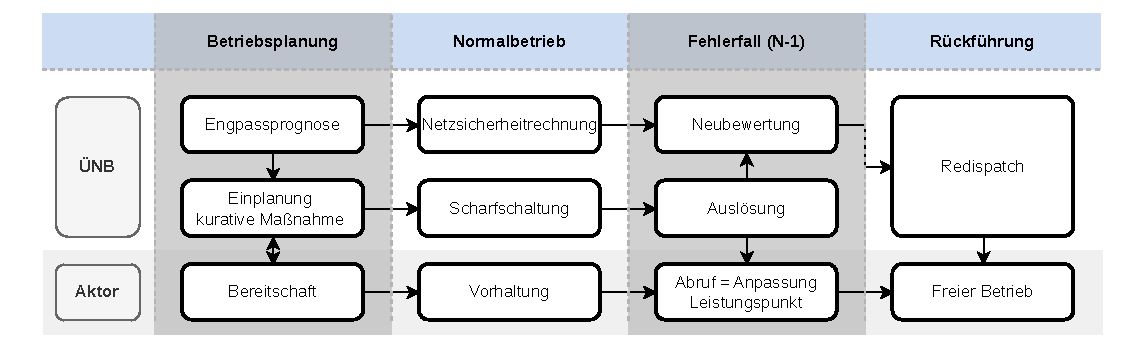
\includegraphics[width=\textwidth]{figures/chapter_2/curative_process.pdf}
    \caption{Prozesskette einer kurativen Maßnahme bei Erbringung durch einen marktlichen Akteur.}
    \label{fig:curativ_process}
\end{figure}

% BEGRIFFSABSATZ eingesetzt am 16.09.2026 auf Vorgabe des Verfassers. Scharfschaltung und Ausloesung nach InnoSys 2030 Abschlussbericht S. 51 (Aktivierung gleich Scharfschaltung, Ausloesekriterien nach der Fehleridentifikation), Abruf dort nicht definiert, aber durchgehend als Anforderung der bereitgestellten Flexibilitaet verwendet (S. 139, 164). Reaktionszeit nach S. 80.
Für die vier Phasen gelten im Folgenden feste Begriffe.
Die Einplanung ist die Auswahl einer kurativen Maßnahme für eine Ausfallvariante in der Betriebsplanung.
Die Scharfschaltung, in InnoSys~2030 Aktivierung genannt, versetzt die eingeplante Maßnahme vor dem Fehler in Einsatzbereitschaft, und die Auslösung ist das Signal des Leitsystems nach dem Eintritt des Fehlers \cite{innosys_2030_gesamtverbund_innovationen_2021}.
Der Abruf ist die Anforderung der zugesagten Leistungsänderung an den Akteur, er beginnt mit der Auslösung und endet mit der Freistellung durch den \ac{ÜNB}.
Die Umsetzung ist die Leistungsänderung, die der Akteur auf den Abruf hin erbringt, und die Reaktionszeit ist die Zeit von der Auslösung bis zur vollständigen Umsetzung.
% DURCHSICHT 15.09.2026, Begriff kurative Bindung, Vorgabe des Verfassers vom 16.09.2026. Alte Fassung:
%Die Bindungsdauer ist der Zeitraum, über den der Akteur die Zusage hält, unabhängig davon, ob ein Abruf erfolgt.
Die kurative Bindung ist die Reservierung eines Leistungsbandes und, bei Speichern, eines Ladezustandsbandes.
Die Bindungsdauer ist der Zeitraum, über den der Akteur die kurative Bindung hält, unabhängig davon, ob ein Abruf erfolgt.

% NEU GEFASST am 15.09.2026 nach dem Absatzplan im Sammelmodus.
% Befunde B63, G17, V4, V9. Aktiviert durch umgesetzt ersetzt, TenneT-Beleg fuer die fuenf Minuten, Befund nicht mehr als positives Pruefergebnis verwendet.
% Alte Fassung, nicht wieder aufnehmen:
%In der Betriebsplanung identifiziert der \ac{ÜNB} auf Basis von Netzprognosen potenzielle Engpässe und überwacht dabei die thermischen Grenzwerte der Betriebsmittel.
%Im Normalbetrieb prüft der \ac{ÜNB} kontinuierlich in der Netzsicherheitsrechnung, ob die geplanten kurativen Maßnahmen bei Eintreten einer Ausfallvariante zur Befundfreiheit führen.
%Bei positivem Befund wird die Maßnahme scharfgeschaltet und der Akteur verbleibt in Bereitschaft.
%Im Fehlerfall löst ein Signal aus dem Leitsystem die scharfgeschaltete Maßnahme aus.
%Im Pilotbetrieb des Projekts KuPilot werden die Maßnahmen vorbereitet und erst nach dem tatsächlichen Eintritt einer Überlastung innerhalb von maximal fünf Minuten automatisiert aktiviert~\cite{tennet_tso_gmbh_pilotbetrieb_2025}.
%Die Akteure passen ihre Leistungspunkte innerhalb der vorgegebenen Reaktionszeit an.
%Der \ac{ÜNB} führt anschließend eine Neubewertung des Systemzustands durch, um die tatsächliche Wirksamkeit der Maßnahme zu überprüfen.
%In der Rückführung veranlasst der \ac{ÜNB} einen Redispatch zur Wiederherstellung des (N-1)-sicheren Zustands.
%Der Akteur wird aus der kurativen Bindung entlassen und kehrt in den freien Betrieb zurück.
In der Betriebsplanung identifiziert der \ac{ÜNB} auf Basis von Netzprognosen mögliche Engpässe und überwacht dabei die thermischen Grenzwerte der Betriebsmittel.
% SATZLAENGE am 15.09.2026, Stilregel 17, alte Fassung als Kommentar:
%Im Normalbetrieb prüft der \ac{ÜNB} in der Netzsicherheitsrechnung fortlaufend, ob die geplanten kurativen Maßnahmen bei Eintreten einer Ausfallvariante den Befund beseitigen, und ist das der Fall, schaltet er die Maßnahme scharf, während der Akteur in Bereitschaft bleibt.
% STATE ESTIMATION HIERHER am 19.09.2026, Kommentar des Verfassers: "die state estimation wird
% in der netzsicherheitsrechnung gemacht und daraus wird ja aktiviert". Der Satz zur State
% Estimation stand bisher beim Absatz zur Betriebsplanung und ist dort gestrichen. Die Quelle
% traegt die Zuordnung woertlich, leeuwen_integration_2020: "Ausfallvarianten der
% Netzbetriebsmittel kontinuierlich in der aktuellen Netzsituation, die bereits umgesetzte
% praeventive Massnahmen einschliesst, durch Leistungsflussrechnungen auf Basis der State
% Estimation ueberprueft. Die Netzsicherheitsrechnung stellt eine wesentliche Informationsquelle
% fuer den Systemfuehrer dar, anhand derer kurzfristige Entscheidungen zur Umsetzung weiterer
% entlastender Massnahmen getroffen werden."
%Im Normalbetrieb prüft der \ac{ÜNB} in der Netzsicherheitsrechnung fortlaufend, ob die geplanten kurativen Maßnahmen bei Eintreten einer Ausfallvariante den Befund beseitigen.
Im Normalbetrieb prüft der \ac{ÜNB} in der Netzsicherheitsrechnung fortlaufend, ob die geplanten kurativen Maßnahmen bei Eintreten einer Ausfallvariante den Befund beseitigen.
Die Netzsicherheitsrechnung stützt sich dabei auf Leistungsflussrechnungen mit der State Estimation, also der aus Messwerten geschätzten Netzsituation \cite{leeuwen_integration_2020}.
Beseitigen die Maßnahmen den Befund, schaltet der \ac{ÜNB} sie scharf.
Der Akteur bleibt dann in Bereitschaft.
% DURCHSICHT 16.09.2026, C1, Einschub als eigener Satz, Stilregel 17. Alte Fassung:
%Im Fehlerfall löst ein Signal aus dem Leitsystem die scharfgeschaltete Maßnahme aus, und im Pilotbetrieb des Projekts KuPilot, in dem Amprion, TenneT und RWE den kurativen Redispatch im realen Betrieb erproben, wird die Leistungsänderung nach dem tatsächlichen Eintritt einer Überlastung innerhalb von fünf Minuten vollständig umgesetzt \cite{tennet_tso_gmbh_pilotbetrieb_2025}.
Im Fehlerfall löst ein Signal aus dem Leitsystem die scharfgeschaltete Maßnahme aus.
% R-19 am 18.09.2026, Kontrolle durch Fable, Entscheidung des Verfassers: der Satz unterbrach die Prozessbeschreibung und steht jetzt in 2.1.4. Alte Fassung:
%Im Pilotbetrieb des Projekts KuPilot, in dem Amprion, TenneT und RWE den kurativen Redispatch im realen Betrieb erproben, wird die Leistungsänderung nach dem tatsächlichen Eintritt einer Überlastung innerhalb von fünf Minuten vollständig umgesetzt \cite{tennet_tso_gmbh_pilotbetrieb_2025}.
Die Akteure setzen ihre Leistungsänderung innerhalb der vorgegebenen Reaktionszeit um, und der \ac{ÜNB} bewertet den Systemzustand anschließend neu, um die Wirksamkeit der Maßnahme zu prüfen.
% BEDINGUNG ERGAENZT am 19.09.2026, Vorgabe des Verfassers: "und sobald weitere Ueberlastungen
% ausgeschlossen sind". Die Entlassung aus der kurativen Bindung war bisher ohne Bedingung
% genannt. Der Satz ist dafuer in drei Saetze geteilt, denn er trug einen Hauptsatz und zwei
% angehaengte Hauptsaetze, und die Bedingung haette einen Nebensatz hinzugefuegt, Stilregel 17.
% Zugleich steht der UeNB jetzt als handelnder Akteur im Subjekt statt im Passiv, Stilregeln 10
% und 12. Alte Fassung:
%In der Rückführung veranlasst der \ac{ÜNB} einen Redispatch zur Wiederherstellung des (N-1)-sicheren Zustands, und der Akteur wird aus der kurativen Bindung entlassen und kehrt in den freien Betrieb zurück.
In der Rückführung veranlasst der \ac{ÜNB} einen Redispatch zur Wiederherstellung des (N-1)-sicheren Zustands.
Sobald weitere Überlastungen ausgeschlossen sind, entlässt der \ac{ÜNB} den Akteur aus der kurativen Bindung.
Der Akteur kehrt dann in den freien Betrieb zurück.

% NEU GEFASST am 15.09.2026 nach dem Absatzplan im Sammelmodus.
% Befunde B64, B65, G18, Q15, P7, B81, B82. PTDF-Satz entfallen, heutige und geplante Mittel des UENB getrennt, Quelle und Senke definiert, Verbund von Zusagen.
% Alte Fassung, nicht wieder aufnehmen:
%N-1-gefährdete Situationen erkennt der \ac{ÜNB}, indem er die Ausfallvarianten der Netzbetriebsmittel fortlaufend in der aktuellen Netzsituation durch Leistungsflussrechnungen auf Basis der State Estimation überprüft \cite{leeuwen_integration_2020}.
%In den Optimierungsmodellen des Engpassmanagements bilden \ac{PTDF}- und \ac{LODF}-Sensitivitäten den Einfluss einer Leistungsänderung beziehungsweise eines Leitungsausfalls auf die Lastflüsse linearisiert ab~\cite{blank_determination_2024}.
%Für kritische Ausfallvarianten identifiziert der \ac{ÜNB} die Möglichkeit einer kurativen Maßnahme zur Engpassbehebung.
%Der dafür dokumentierte Maßnahmenraum reicht von leistungsflusssteuernden Betriebsmitteln bis zu Eingriffen in Erzeugung und Last \cite{innosys_2030_gesamtverbund_innovationen_2021}, und die Maßnahmen unterscheiden sich darin, wer über das eingesetzte Betriebsmittel verfügt.
%Schaltmaßnahmen, die Sollwertanpassung leistungsflusssteuernder Betriebsmittel wie \ac{PST} und \ac{HGÜ} sowie der Einsatz von Netzboostern liegen im Verfügungsbereich des \ac{ÜNB} selbst und erfordern keine Zusage eines Dritten \cite{consentec_systembooster_2026}.
%Eingriffe in Erzeugung, Last und Speicherung setzen demgegenüber voraus, dass ein Anlagenbetreiber die geforderte Leistungsänderung zusagt und zum Abrufzeitpunkt erbringt.
%Nur bei den Maßnahmen der zweiten Gruppe stellt sich die Frage nach Vorhaltung und Vergütung, weshalb die weitere Betrachtung auf sie beschränkt bleibt.
%Der Akteur meldet dem \ac{ÜNB} sein verfügbares Hoch- und Runterfahrpotenzial, das heißt die positive und negative Leistungsänderung, die er innerhalb der geforderten Reaktionszeit bereitstellen kann.
%Bei energiebegrenzten Technologien wie Speichern ist darüber hinaus sicherzustellen, dass zum Zeitpunkt eines möglichen Abrufs ausreichend gespeicherte Energie zur Verfügung steht.
%Dies erfordert eine gezielte Vorhaltung des Ladezustands im Vorfeld des Abrufs.
%Für den bilanziellen Ausgleich einer kurativen Maßnahme sind mindestens zwei Akteure erforderlich, die als Quelle und Senke koordiniert eingesetzt werden.
%Für die Beschaffung folgt daraus, dass an einem Netzknoten nicht eine einzelne Zusage, sondern ein aufeinander abgestimmtes Paar von Zusagen erforderlich ist.
% R-20 am 18.09.2026, Kontrolle durch Fable, Entscheidung des Verfassers: Satz geteilt, Stilregel 17. Alte Fassung:
%Grundlage der Betriebsplanung ist die Erkennung gefährdeter Zustände, die der \ac{ÜNB} leistet, indem er die Ausfallvarianten der Netzbetriebsmittel fortlaufend in der aktuellen Netzsituation durch Leistungsflussrechnungen auf Basis der State Estimation, also der aus Messwerten geschätzten Netzsituation, überprüft \cite{leeuwen_integration_2020}.
% ZUORDNUNG BERICHTIGT am 19.09.2026, Kommentar des Verfassers: "nein die state estimation wird
% in der netzsicherheitsrechnung gemacht ... in der betriebsplanung wird mittels eines
% synthetischen netzes und prognostizierten einspeise und last situation eine lastflussberechnung
% mit ausfallapproximation gemacht. daraus werden engpaesse identifiziert die dann mit einem pRD
% Tool effizient geloest werden." Die alte Fassung hatte den Satz der Quelle zur
% Netzsicherheitsrechnung woertlich uebernommen und als Betriebsplanung ausgewiesen, also die
% Echtzeitrechnung mit der Planungsrechnung verwechselt. leeuwen_integration_2020 zur
% Betriebsplanung: "Innerhalb dieser Prozesse werden Optimierungsalgorithmen genutzt, die auf
% Basis von Prognosen der Netznutzung potentielle Engpaesse sowie moegliche Entlastungsmassnahmen
% ermitteln", und "Alle Betriebsplanungsprozesse basieren auf Prognosen (fuer EE-Einspeisung,
% Last, Netztopologie, Kraftwerkseinspeisung, etc.), die laufend aktualisiert werden." Die Quelle
% nennt als Prozesse WAPP, pRD1, pRD2/DACF und IDCF und in Fussnote 10 als Verfahren den
% AC-SCOPF. Die vom Verfasser genannten Begriffe synthetisches Netz und Ausfallapproximation
% stehen nicht in dieser Quelle und sind deshalb nicht uebernommen; der Text bleibt beim Wortlaut
% der Quelle. Alte Fassung, nicht wieder aufnehmen:
%Grundlage der Betriebsplanung ist die Erkennung gefährdeter Zustände, für die der \ac{ÜNB} die Ausfallvarianten der Netzbetriebsmittel fortlaufend in der aktuellen Netzsituation prüft \cite{leeuwen_integration_2020}.
Grundlage der Betriebsplanung ist die Erkennung gefährdeter Zustände, für die der \ac{ÜNB} die Ausfallvarianten der Netzbetriebsmittel prüft \cite{leeuwen_integration_2020}.
Die Prüfung beruht auf Prognosen der Netznutzung, nämlich für die Einspeisung aus erneuerbaren Energien, die Last, die Netztopologie und die Einspeisung der Kraftwerke.
Optimierungsalgorithmen ermitteln daraus die potenziellen Engpässe und die möglichen Entlastungsmaßnahmen.
% GESTRICHEN am 19.09.2026, siehe den Kommentar zum Absatz davor: der Satz beschreibt die
% Netzsicherheitsrechnung und steht jetzt dort. Gestrichener Satz:
%Die Prüfung beruht auf Leistungsflussrechnungen mit der State Estimation, also der aus Messwerten geschätzten Netzsituation.
Für kritische Ausfallvarianten identifiziert der \ac{ÜNB} die Möglichkeit einer kurativen Maßnahme zur Engpassbehebung, und der dafür dokumentierte Maßnahmenraum reicht von leistungsflusssteuernden Betriebsmitteln bis zu Eingriffen in Erzeugung und Last \cite{innosys_2030_gesamtverbund_innovationen_2021}, wobei sich die Maßnahmen darin unterscheiden, wer über das eingesetzte Betriebsmittel verfügt.
% S-17 am 18.09.2026, Kontrolle durch Fable, Entscheidung des Verfassers: gestrichen, die Aussage traegt 2.1.4. Gestrichener Satz: Alte Fassung:
%Heute verfügbar sind auf Seiten des \ac{ÜNB} Topologieschaltmaßnahmen und die Sollwertanpassung leistungsflusssteuernder Betriebsmittel wie \ac{PST}, während die innerdeutschen \ac{HGÜ}-Korridore und die Netzbooster, die speicherbasierte Leistung für den Fehlerfall vorhalten sollen, noch in der Umsetzung sind \cite{consentec_systembooster_2026}.
% BEGRIFF am 20.09.2026, Vorgabe des Verfassers: EIV statt Anlagenbetreiber, weil hier die Rolle gemeint ist,
% die den Fahrplan bestimmt und die Zusage gibt. Alte Fassung:
%Maßnahmen mit eigenen Betriebsmitteln erfordern keine Zusage eines Dritten, während Eingriffe in Erzeugung, Last und Speicherung voraussetzen, dass ein Anlagenbetreiber die geforderte Leistungsänderung zusagt und zum Abrufzeitpunkt erbringt.
Maßnahmen mit eigenen Betriebsmitteln erfordern keine Zusage eines Dritten, während Eingriffe in Erzeugung, Last und Speicherung voraussetzen, dass ein \ac{EIV} die geforderte Leistungsänderung zusagt und zum Abrufzeitpunkt erbringt.
Nur bei Eingriffen in Erzeugung, Last und Speicherung stellt sich die Frage nach Vorhaltung und Vergütung, weshalb die weitere Betrachtung auf sie beschränkt bleibt.
% SATZLAENGE am 15.09.2026, Stilregel 17, alte Fassung als Kommentar:
%Der Akteur meldet dem \ac{ÜNB} sein verfügbares Hoch- und Runterfahrpotenzial, also die positive und die negative Leistungsänderung, die er innerhalb der geforderten Reaktionszeit bereitstellen kann, und bei energiebegrenzten Technologien wie Speichern ist darüber hinaus sicherzustellen, dass zum Zeitpunkt eines möglichen Abrufs ausreichend gespeicherte Energie zur Verfügung steht, was eine gezielte Vorhaltung des Ladezustands im Vorfeld verlangt.

% NEUER ABSATZ 16.09.2026, C2.5.
% DURCHSICHT 16.09.2026, C1, Anknuepfung. Alte Fassung:
%Der Akteur meldet dem \ac{ÜNB} sein verfügbares Hoch- und Runterfahrpotenzial, also die positive und die negative Leistungsänderung, die er innerhalb der geforderten Reaktionszeit bereitstellen kann.
Für eine solche Zusage meldet der Akteur dem \ac{ÜNB} sein verfügbares Hoch- und Runterfahrpotenzial, also die positive und die negative Leistungsänderung, die er innerhalb der geforderten Reaktionszeit bereitstellen kann.
% GESTRICHEN am 19.09.2026, Kommentar des Verfassers zur Dopplung. Die Aussage steht bereits
% acht Zeilen vorher als Begriffsbestimmung ("Die kurative Bindung ist die Reservierung eines
% Leistungsbandes und, bei Speichern, eines Ladezustandsbandes"), in 2.1.1 ("er haelt Leistung
% und Ladezustandsbereich fuer einen ungewissen Abruf frei") und systematisch in 2.1.3, wo die
% Energiebindung eines von vier Vergleichsmerkmalen ist. Gestrichene Saetze:
%Bei energiebegrenzten Technologien wie Speichern ist darüber hinaus sicherzustellen, dass zum Zeitpunkt eines möglichen Abrufs ausreichend gespeicherte Energie zur Verfügung steht.
%Die Sicherstellung verlangt eine gezielte Vorhaltung des Ladezustands im Vorfeld.
% SATZLAENGE am 15.09.2026, Stilregel 17, alte Fassung als Kommentar:
%Eine marktbezogene kurative Maßnahme wird in der Regel bilanziell ausgeglichen, sodass die Summe der Einspeisung unverändert bleibt, wobei die Anlage, die ihre Einspeisung erhöht, als Quelle und die Anlage, die ihre Einspeisung senkt, als Senke wirkt, sodass an einem Netzknoten nicht eine einzelne Zusage, sondern ein Verbund von Zusagen erforderlich ist.
% DURCHSICHT 16.09.2026, C1. Alte Fassung:
%Eine marktbezogene kurative Maßnahme wird in der Regel bilanziell ausgeglichen, sodass die Summe der Einspeisung unverändert bleibt.
Die Zusage steht zudem nicht allein, denn eine marktbezogene kurative Maßnahme wird in der Regel bilanziell ausgeglichen, sodass die Summe der Einspeisung unverändert bleibt.
Die Anlage mit erhöhter Einspeisung wirkt dabei als Quelle, die Anlage mit gesenkter Einspeisung als Senke.
An einem Netzknoten ist deshalb nicht eine einzelne Zusage, sondern ein Verbund von Zusagen erforderlich.
% NEU GEFASST am 15.09.2026 nach dem Absatzplan im Sammelmodus.
% Befunde B66, B67, B68, A2, Q10, Q11, V6. Waermebilanz, Joule-Gleichung, Beispiel und Abbildung in Anhang anh:thermik verschoben, Hauptteil auf fuenf Saetze.
% Alte Fassung, nicht wieder aufnehmen:
%Die Anforderungen an die Aktivierungsgeschwindigkeit ergeben sich unmittelbar aus dem \ac{TATL}-Zeitfenster des jeweils betroffenen Betriebsmittels.
%Dessen Dauer ist keine Konstante des Betriebsmittels, sondern folgt aus dessen Wärmebilanz.
%Da Wärmekapazität und Kühlmechanismen von der Bauart abhängen, liegen die Zeitkonstanten verschiedener Betriebsmittel um Größenordnungen auseinander, weshalb die Darstellung im Folgenden an der Freileitung erfolgt.
%Die Wärmebilanz einer Freileitung lautet in der für eine Überlast maßgeblichen transienten Form nach \cite{cigre_thermal_2014}
%\begin{equation}
%    m\,c_{\mathrm{p}}\,\frac{\mathrm{d}\vartheta}{\mathrm{d}t} = P_{\mathrm{J}}(I,\vartheta) + P_{\mathrm{S}} - P_{\mathrm{C}}(\vartheta,\vartheta_{\mathrm{u}},v_{\mathrm{w}},\delta) - P_{\mathrm{R}}(\vartheta,\vartheta_{\mathrm{u}})
%    \label{eq:waermebilanz}
%\end{equation}
%mit der mittleren Leitertemperatur $\vartheta$, der Wärmekapazität $m\,c_{\mathrm{p}}$, der ohmschen Verlustwärme $P_{\mathrm{J}}$, dem solaren Eintrag $P_{\mathrm{S}}$, der konvektiven und der Strahlungskühlung $P_{\mathrm{C}}$ und $P_{\mathrm{R}}$ sowie dem Anströmwinkel des Windes $\delta$.
%Magnetische Erwärmung und Verdunstungskühlung sind dabei nicht aufgeführt, und die Wärmekapazität ist als konstant angesetzt.
%Gleichung~\ref{eq:waermebilanz} beschreibt damit einen blanken Leiter im Freien.

%Die Kühlung hängt von den Wetterbedingungen ab und wächst unterproportional mit der Windgeschwindigkeit, weshalb windschwache Stunden den engsten Fall bilden \cite{cigre_thermal_2014}.
%Dieses witterungsabhängige Potenzial wird bereits durch das Freileitungsmonitoring erschlossen, das den dauerhaft zulässigen Grenzwert an die tatsächlich vorliegenden Bedingungen anpasst \cite{dena_hoeherauslastung_2022}.
%Die kurative Höherauslastung setzt demgegenüber auf der Erwärmungsseite an, denn die ohmsche Verlustwärme wächst bei gegebener Leitertemperatur quadratisch mit dem Strom und lautet
%\begin{equation}
%    P_{\mathrm{J}}(I,\vartheta) = I^{2}\,R'_{20}\left[1 + \alpha_{20}\left(\vartheta - \vartheta_{20}\right)\right]
%    \label{eq:jouleverluste}
%\end{equation}
%mit dem längenbezogenen Widerstand $R'_{20}$ bei der Bezugstemperatur $\vartheta_{20}$ und dem Temperaturkoeffizienten $\alpha_{20}$.
%Vernachlässigt sind dabei der Skineffekt, also die Verdrängung des Stroms an den äußeren Rand des Leiterseils, die den wirksamen Widerstand bei Wechselstrom erhöht, sowie die Nichtlinearität des Widerstands bei hohen Temperaturen.
%Eine Erhöhung des Stroms um zehn Prozent steigert den Wärmeeintrag nach Gleichung~\ref{eq:jouleverluste} damit um rund ein Fünftel.
%Genutzt wird dabei nicht die stationäre Kühlung, sondern die Wärmekapazität des Betriebsmittels, die einen Strom oberhalb des Dauergrenzwerts für eine begrenzte Zeit zulässt.
%Bei einer Überlast überwiegt der Wärmeeintrag, und die Leitertemperatur steigt.
%Ihr Ausgangswert folgt dabei aus der Vorbelastung, und sie strebt derjenigen Temperatur zu, bei der sich Wärmeeintrag und Kühlung wieder ausgleichen.
%Die Überlast ist zulässig, bis die Grenztemperatur erreicht ist, und aus dieser Dauer folgt die der jeweiligen Überlasthöhe zugeordnete zulässige Dauer.
%Abbildung \ref{fig:tatl_berechnung} zeigt die Eingangsgrößen und den daraus folgenden Temperaturverlauf.

%\begin{figure}[htbp]
%    \centering
% GROESSENANGABE ERGAENZT am 12.09.2026 nach der Anweisung des Verfassers.
% Sie aendert den Satz nicht, die Datei ist genau textbreit.
%    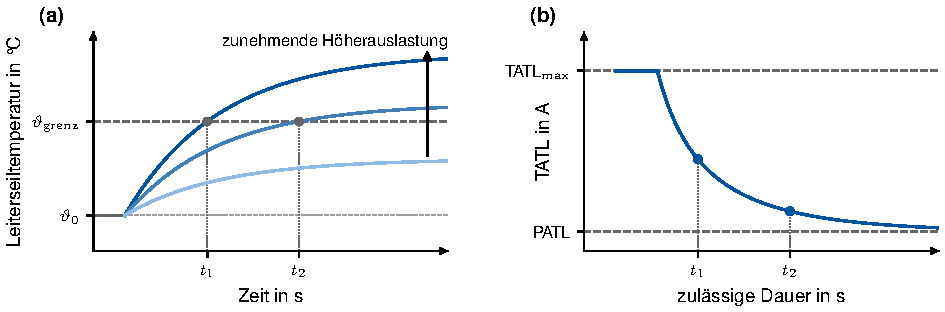
\includegraphics[width=\textwidth]{figures/chapter_2/tatl_berechnung.pdf}
%    \caption{Schematische Darstellung der zulässigen Überlastdauer einer Freileitung. Teilbild a zeigt die Temperaturverläufe für drei Überlasthöhen, Teilbild b die daraus folgende Kennlinie aus zulässiger Belastbarkeit und zulässiger Dauer.}
%    \label{fig:tatl_berechnung}
%\end{figure}

%Für Transformatoren gilt derselbe Mechanismus, allerdings mit drei Unterschieden in der Ausprägung.
%Maßgebliche Größe ist dort nicht die Temperatur des stromführenden Leiters selbst, sondern die Heißpunkttemperatur der Wicklung, die über die Öltemperatur und den Ölumlauf mit der Umgebung verbunden ist.
%Zwischen der Verlustentstehung in der Wicklung und der Wärmeabgabe an die Umgebungsluft liegt damit ein zusätzlicher innerer Transportweg.
%Die Wärmekapazität eines Transformators ist größer, weshalb die zulässigen Überlastdauern länger ausfallen als bei einer Freileitung.
%Hinzu kommt, dass eine Überlast dort nicht allein das Erreichen einer Grenztemperatur riskiert, sondern über die Heißpunkttemperatur die Alterung der Isolation beschleunigt und einen Anteil der Lebensdauer verbraucht, sodass neben der Höhe und der Dauer auch die Häufigkeit der Überlastung zu begrenzen ist \cite{iec_60076_7_2018}.
%Für eine Übertragungsstrecke ist folglich das Minimum der zulässigen Dauern über alle betroffenen Betriebsmittel maßgeblich, weshalb zwischen dem thermisch bestimmten Grenzwert eines einzelnen Betriebsmittels und dem für die Betriebsführung nutzbaren Grenzwert zu unterscheiden ist \cite{dena_hoeherauslastung_2022}.
% SATZLAENGE am 15.09.2026, Stilregel 17, alte Fassung als Kommentar:
%Die Anforderungen an die Reaktionszeit ergeben sich aus dem \ac{TATL}-Zeitfenster des betroffenen Betriebsmittels, dessen Dauer keine Konstante des Betriebsmittels ist, sondern aus dessen Wärmebilanz folgt: Bei einer Überlast überwiegt der Wärmeeintrag die Kühlung, die Temperatur steigt von dem Ausgangswert an, den die Belastung vor dem Ausfall bestimmt, und die Überlast ist zulässig, bis die Grenztemperatur erreicht ist.
% DURCHSICHT 16.09.2026, C1, Anknuepfung. Alte Fassung:
%Die Anforderungen an die Reaktionszeit ergeben sich aus dem \ac{TATL}-Zeitfenster des betroffenen Betriebsmittels.
Wie schnell ein solcher Verbund wirken muss, ergibt sich aus dem \ac{TATL}-Zeitfenster des betroffenen Betriebsmittels.
Die Dauer des Zeitfensters ist keine Konstante des Betriebsmittels, sondern folgt aus der Wärmebilanz.
% R-21 am 18.09.2026, Kontrolle durch Fable, Entscheidung des Verfassers: drei Saetze zu einem verbunden, S-06. Alte Fassung:
%Bei einer Überlast überwiegt der Wärmeeintrag die Kühlung.
% GESTRICHEN am 19.09.2026, Kommentar des Verfassers: "die infos wuerde ich fast streichen, da
% sie auch in dieser arbeit eher nebensaechlich sind. zu dem davor." Der Temperaturverlauf steht
% nahezu woertlich in Anhang B, extras/attachment_thermik.tex: "Bei einer Ueberlast ueberwiegt
% der Waermeeintrag, und die Leitertemperatur steigt vom Ausgangswert der Vorbelastung an." Der
% Absatz verweist selbst auf den Anhang. Gestrichener Satz:
%Bei einer Überlast überwiegt der Wärmeeintrag die Kühlung, und die Temperatur steigt vom Ausgangswert der Vorbelastung bis zur Grenztemperatur, bis zu der die Überlast zulässig ist.
% S-06 am 18.09.2026, Kontrolle durch Fable, Entscheidung des Verfassers: in den vorigen Satz aufgenommen. Alter Satz: Alte Fassung:
%Die Temperatur steigt dann von dem Ausgangswert an, den die Belastung vor dem Ausfall bestimmt.
% S-06 am 18.09.2026, Kontrolle durch Fable, Entscheidung des Verfassers: in den vorigen Satz aufgenommen. Alter Satz: Alte Fassung:
%Die Überlast ist zulässig, bis die Grenztemperatur erreicht ist.
% GESTRICHEN am 19.09.2026, derselbe Kommentar. Die Abhaengigkeit von Vorbelastung und Witterung
% bleibt im Text erhalten, naemlich im Absatz zur wechselseitigen Bindung ("je nach Vorbelastung
% und Wetterlage unterschiedlich") und in 2.1.4 ("neben der Strecke bestimmen Vorbelastung und
% Witterung die zulaessige Dauer"). Der Beleg cigre_thermal_2014 bleibt in Anhang B in Gebrauch.
% Gestrichener Satz:
%Die zulässige Dauer hängt deshalb von der Vorbelastung und von der Witterung ab und ist in windschwachen Stunden am kürzesten, weil die Kühlung mit der Windgeschwindigkeit wächst \cite{cigre_thermal_2014}.
% GESTRICHEN am 19.09.2026, derselbe Kommentar. Die Alterung der Isolation steht in Anhang B:
% "Die Ueberlastung aeussert sich am Leiterseil durch Durchhang und Festigkeit und am
% Transformator durch die Alterung der Isolation." Der Beleg iec_60076_7_2018 bleibt dort in
% Gebrauch. Die Begrenzung der Haeufigkeit entfaellt damit aus dem Kapitel; sie ist fuer die
% Fragestellung ohne Folge, weil die Arbeit die Haeufigkeit des Abrufs nicht modelliert.
% Gestrichener Satz:
%Bei Transformatoren ist die zulässige Dauer wegen der größeren Wärmekapazität länger, zugleich beschleunigt die Überlast dort die Alterung der Isolation, sodass neben Höhe und Dauer auch die Häufigkeit der Überlastung zu begrenzen ist \cite{iec_60076_7_2018}.
Für eine Übertragungsstrecke ist das Minimum der zulässigen Dauern über alle betroffenen Betriebsmittel maßgeblich, weshalb der für die Betriebsführung nutzbare Grenzwert unter dem thermischen Grenzwert des einzelnen Betriebsmittels liegen kann \cite{dena_hoeherauslastung_2022}.
% NEU GEFASST am 17.09.2026: der Anhang stellt den Vergleich mit dem Transformator nicht mehr dar, der Verweis darf ihn nicht ankuendigen. Alte Fassung:
%Anhang~\ref{anh:thermik} stellt die Wärmebilanz der Freileitung, die Berechnung der zulässigen Dauer und die Unterschiede beim Transformator dar.
% I-27 am 18.09.2026, Kontrolle durch Fable, Entscheidung des Verfassers: der Anhang traegt seit der Kuerzung keine Rechnung. Alte Fassung:
%Anhang~\ref{anh:thermik} stellt die Wärmebilanz der Freileitung und die Berechnung der zulässigen Dauer dar.
% R-75 am 18.09.2026, Kontrolle durch Fable, Entscheidung des Verfassers: Anhaenge handeln nicht, Stilregel 10. Alte Fassung:
%Anhang~\ref{anh:thermik} stellt die Wärmebilanz der Freileitung und den Temperaturverlauf bei einer Überlast dar.
Die Wärmebilanz der Freileitung und der Temperaturverlauf bei einer Überlast stehen in Anhang~\ref{anh:thermik}.

% NEU GEFASST am 15.09.2026 nach dem Absatzplan im Sammelmodus.
% Befunde B69, G20, Q12, V4, V8. Grenzwertkonzept als Beleg fuer die weiteren Bedingungen, Saetze verbunden, Wirksamkeit statt Aktivierungsgeschwindigkeit.
% Alte Fassung, nicht wieder aufnehmen:
%Aus dieser Berechnungslogik folgt eine wechselseitige Bindung zwischen dem gewählten Betriebspunkt und der Technologie des Akteurs.
%Eine weitergehende Höherauslastung erschließt ein größeres Entlastungspotenzial und verkürzt zugleich das Zeitfenster für die Gegenmaßnahme, und die zulässige Dauer fällt für dasselbe Betriebsmittel je nach Vorbelastung und Wetterlage unterschiedlich aus \cite{sous_comparison_2025}.
%Der Akteur kann die ihm verbleibende Reaktionszeit deshalb nicht selbst bestimmen, sie ergibt sich aus dem Betriebsmittel und der Situation.
%Die Höherauslastung wiederum ist nur so weit zulässig, wie das Überlastintervall für die Reaktionszeit des Akteurs ausreicht.
%Damit der \ac{ÜNB} den Betriebspunkt planen kann, muss der Akteur deshalb auf eine feste Reaktionszeit festgelegt sein.

%InnoSys~2030 systematisiert die kurativen Maßnahmen entlang dieser Spanne in drei Klassen, nämlich sehr schnelle Maßnahmen mit einer Wirksamkeit von unter zehn Sekunden, schnelle Maßnahmen mit einer Wirksamkeit von etwa zwei Minuten und langsame Maßnahmen mit einer Wirksamkeit von bis zu 15 Minuten \cite{innosys_2030_gesamtverbund_innovationen_2021}.
%Sie bilden die erreichbare Aktivierungsgeschwindigkeit ab, während die im Einzelfall maßgebliche Dauer der \ac{ÜNB} nach Art.\,25 \ac{SOGL} festlegt.
%Die zugesagte Reaktionszeit geht deshalb als Bedingung in die Einsatzplanung ein, denn eine verspätete Maßnahme entlastet das Betriebsmittel nicht mehr rechtzeitig \cite{lindner_operation_2023}.
% R-22 am 18.09.2026, Kontrolle durch Fable, Entscheidung des Verfassers: Satz geteilt, Stilregel 17. Alte Fassung:
%Aus der Wärmebilanz folgt eine wechselseitige Bindung zwischen dem gewählten Betriebspunkt und der Technologie des Akteurs: Eine weitergehende Höherauslastung erschließt ein größeres Entlastungspotenzial und verkürzt zugleich das Zeitfenster für die Gegenmaßnahme, und die zulässige Dauer fällt für dasselbe Betriebsmittel je nach Vorbelastung und Wetterlage unterschiedlich aus \cite{sous_comparison_2025}.
Aus der Wärmebilanz folgt eine wechselseitige Bindung zwischen dem gewählten Betriebspunkt und der Technologie des Akteurs, denn eine weitergehende Höherauslastung erschließt ein größeres Entlastungspotenzial und verkürzt zugleich das Zeitfenster für die Gegenmaßnahme.
Die zulässige Dauer fällt zudem für dasselbe Betriebsmittel je nach Vorbelastung und Wetterlage unterschiedlich aus \cite{sous_comparison_2025}.
Der Akteur kann die ihm verbleibende Reaktionszeit deshalb nicht selbst bestimmen, denn sie ergibt sich aus dem Betriebsmittel und der Situation, und damit der \ac{ÜNB} den Betriebspunkt planen kann, muss der Akteur auf eine feste Reaktionszeit festgelegt sein.
% S-18 am 18.09.2026, Kontrolle durch Fable, Entscheidung des Verfassers: die Aufzaehlung der weiteren Grenzwerte steht in 2.1.4 Absatz 29. Alte Fassung:
%Die Höherauslastung ist umgekehrt nur zulässig, soweit der \ac{ÜNB} den Stromkreis dafür freigegeben hat, die zulässige Überlastdauer die Reaktionszeit des Akteurs deckt und die weiteren Grenzwerte des Grenzwertkonzepts der deutschen \ac{ÜNB}, nämlich Schutz, Spannung, Stabilität und Genehmigungen etwa zum Immissionsschutz, eingehalten sind \cite{uenb_grenzwertkonzept_2021}.
Die Höherauslastung ist umgekehrt nur zulässig, soweit der \ac{ÜNB} den Stromkreis dafür freigegeben hat und die zulässige Überlastdauer die Reaktionszeit des Akteurs deckt \cite{uenb_grenzwertkonzept_2021}.
% DURCHSICHT 16.09.2026, C1, Bezug. Alte Fassung:
%InnoSys~2030 systematisiert die kurativen Maßnahmen entlang dieser Spanne nach der Zeit bis zur vollen Entlastungswirkung in drei Klassen, nämlich sehr schnelle Maßnahmen mit einer Wirksamkeit von unter zehn Sekunden, schnelle Maßnahmen mit einer Wirksamkeit von etwa zwei Minuten und langsame Maßnahmen mit einer Wirksamkeit von bis zu 15 Minuten \cite{innosys_2030_gesamtverbund_innovationen_2021}.
% R-22 am 18.09.2026, Kontrolle durch Fable: der Absatz trug zwei Thesen, hier beginnt die zweite.

% BEZUG BERICHTIGT am 19.09.2026, Befund der Zahlenpruefung: die drei Klassen gehoeren dem Netz und
% nicht den Massnahmen. InnoSys 2030, S. 34: "Im Projekt wurden drei TATL Zeitfenster definiert,
% welche sich an den Moeglichkeiten der Betriebsmittel hinsichtlich Schnelligkeit der Aktivierung
% orientieren", naemlich "Ein Zeitfenster <10s (Arbeitshypothese 1s, 'sehr schnell')", "ein
% Zwei-Minuten-Zeitfenster ('schnell')" und "ein 15-Minuten-Zeitfenster ('langsam')". Die drei
% Zahlen sind damit woertlich bestaetigt, die alte Fassung drehte allein die Richtung der Aussage
% um. Zugleich BELEG BERICHTIGT: Art. 25 Abs. 1 lit. c SO GL verpflichtet den UeNB zur Festlegung
% der "Grenzwerte fuer den Strom hinsichtlich der thermischen Belastbarkeit, einschliesslich
% voruebergehend zulaessiger Ueberlastungen"; die zulaessige Dauer selbst benennt erst Art. 35
% Abs. 2 mit Rueckverweis auf Art. 25 Abs. 1 lit. c. Der Satz bezieht sich deshalb jetzt auf die
% Grenzwerte und nicht mehr auf die Dauer. Alte Fassung, nicht wieder aufnehmen:
%InnoSys~2030 systematisiert die kurativen Maßnahmen nach der Zeit bis zur vollen Entlastungswirkung in drei Klassen, nämlich sehr schnelle Maßnahmen mit einer Wirksamkeit von unter zehn Sekunden, schnelle Maßnahmen mit einer Wirksamkeit von etwa zwei Minuten und langsame Maßnahmen mit einer Wirksamkeit von bis zu 15 Minuten \cite{innosys_2030_gesamtverbund_innovationen_2021}.
%Die Klassen bilden die erreichbare Zeit bis zur Wirkung ab, während die im Einzelfall maßgebliche Dauer der \ac{ÜNB} nach Art.\,25 \ac{SOGL} festlegt.
InnoSys~2030 definiert drei Zeitfenster für die vorübergehend zulässige Überlast, an denen sich die kurativen Maßnahmen ausrichten, nämlich ein sehr schnelles unter zehn Sekunden, ein schnelles von etwa zwei Minuten und ein langsames von bis zu 15 Minuten \cite{innosys_2030_gesamtverbund_innovationen_2021}.
Die Zeitfenster geben vor, wie schnell eine Maßnahme wirken muss.
Die im Einzelfall zulässige Überlastdauer folgt dagegen aus den Grenzwerten, die der \ac{ÜNB} nach Art.\,25 \ac{SOGL} festlegt.
Die zugesagte Reaktionszeit geht deshalb als Bedingung in die Einsatzplanung ein, denn eine verspätete Maßnahme entlastet das Betriebsmittel nicht mehr rechtzeitig \cite{lindner_operation_2023}.

\subsection{Technologien kurativer Akteure}
\label{sec:curative_actors}
\label{sec:curative_technologies}
\label{sec:actor_comparison}

% NEU GEFASST am 15.09.2026 nach dem Absatzplan im Sammelmodus.
% Befunde B70 bis B77, G22. Mechanismus benannt, vier Merkmale einmal gezaehlt, Bemessungsgrundlage erklaert, netzseitige Betriebsmittel, Tabelle folgt dem Verweis.
% Alte Fassung, nicht wieder aufnehmen:
%Die kurative Maßnahme ist nach Abschnitt \ref{sec:curative_functionality} auf die Zusage eines Anlagenbetreibers angewiesen, sobald sie über eine Anlage erbracht wird, die kein Betriebsmittel des \ac{ÜNB} ist.
%Damit stellt sich die Frage, welche Technologie eine solche Zusage einlösen kann.
%Der Mechanismus soll dabei die Anlagen erreichen, die eine kurative Zusage am verlässlichsten einlösen, ohne einzelne Technologien vom Zugang auszuschließen.
%Beides zugleich ist nur zu erreichen, wenn er nicht an der Technologie ansetzt, sondern an den Eigenschaften, auf die es ankommt.
%Der folgende Vergleich stützt sich auf zwei Eigenschaften der Anlage, nämlich die erreichbare Reaktionszeit und die Frage, ob die Bereitstellung eine Bindung von Energie und nicht nur von Leistung erfordert.
%Ihnen stellt er den Bestand und seine Entwicklung gegenüber, weil davon abhängt, wie viele geeignete Anbieter an einem Netzknoten zu erwarten sind.
%Hinzu tritt als viertes Merkmal der Vergütungspfad, über den ein Eingriff im geltenden Regulierungsrahmen abgerechnet würde.
%Er betrifft nicht die Eignung der Technologie, sondern die Frage, ob für sie bereits eine Bemessungsgrundlage besteht.
%Tabelle~\ref{tab:akteursvergleich} stellt die in Betracht kommenden Technologien entlang dieser Merkmale gegenüber.
%Die Systematisierung folgt der Flexibilitätstypologie nach Erzeugung, Verbrauch, Speicherung und Netz \cite{vde_etg_flexibilisierung_2023} sowie dem Maßnahmenkatalog aus InnoSys~2030 \cite{innosys_2030_gesamtverbund_innovationen_2021}.
% BEGRIFF am 20.09.2026, Vorgabe des Verfassers: EIV statt Anlagenbetreiber, weil hier die Rolle gemeint ist,
% die den Fahrplan bestimmt und die Zusage gibt. Alte Fassung:
%Wird eine kurative Maßnahme über eine Anlage erbracht, die nicht dem \ac{ÜNB} gehört, braucht der \ac{ÜNB} dafür die Zusage des Anlagenbetreibers.
Wird eine kurative Maßnahme über eine Anlage erbracht, die nicht dem \ac{ÜNB} gehört, braucht der \ac{ÜNB} dafür die Zusage des \ac{EIV}.
Damit stellt sich die Frage, welche Technologie eine solche Zusage einlösen kann.
% SATZLAENGE am 15.09.2026, Stilregel 17, alte Fassung als Kommentar:
%Der kurative Marktmechanismus soll die Anlagen erreichen, die eine kurative Zusage am verlässlichsten einlösen, ohne einzelne Technologien vom Zugang auszuschließen, und beides zugleich ist nur zu erreichen, wenn der kurative Marktmechanismus nicht an der Technologie ansetzt, sondern an den Eigenschaften, auf die es ankommt.
% DURCHSICHT 16.09.2026, C1. Alte Fassung:
%Der kurative Marktmechanismus soll die Anlagen erreichen, die eine kurative Zusage am verlässlichsten einlösen, ohne einzelne Technologien vom Zugang auszuschließen.
Der kurative Marktmechanismus soll dafür die Anlagen erreichen, die eine kurative Zusage am verlässlichsten einlösen, ohne einzelne Technologien vom Zugang auszuschließen.
Beides zugleich ist nur zu erreichen, wenn der kurative Marktmechanismus nicht an der Technologie ansetzt, sondern an den maßgeblichen Eigenschaften.
% SATZLAENGE am 15.09.2026, Stilregel 17, alte Fassung als Kommentar:
%Der folgende Vergleich stützt sich deshalb auf vier Merkmale, nämlich die erreichbare Reaktionszeit, die Frage, ob die Bereitstellung eine Bindung von Energie und nicht nur von Leistung erfordert, gemessen am Energieinhalt je Leistung, also der Zeit in Stunden, über die eine Anlage ihre Nennleistung liefern kann, den Anlagenbestand mit seiner Entwicklung, weil davon abhängt, wie viele geeignete Anbieter an einem Netzknoten zu erwarten sind, und den Vergütungspfad, über den ein Eingriff im geltenden Regulierungsrahmen abgerechnet würde.

% NEUER ABSATZ 16.09.2026, C2.6.
Der folgende Vergleich stützt sich deshalb auf vier Merkmale.
Das erste Merkmal ist die erreichbare Reaktionszeit.
Das zweite Merkmal ist die Energiebindung, also ob die Bereitstellung eine Bindung von Energie und nicht nur von Leistung erfordert, gemessen am Energieinhalt je Leistung.
Der Energieinhalt je Leistung ist die Zeit in Stunden, über die eine Anlage ihre Nennleistung liefern kann.
Das dritte Merkmal ist der Anlagenbestand mit seiner Entwicklung, denn der Bestand bestimmt die Zahl der geeigneten Anbieter an einem Netzknoten.
Das vierte Merkmal ist der Vergütungspfad, über den ein Eingriff im geltenden Regulierungsrahmen abgerechnet würde.
Der Vergütungspfad betrifft nicht die Eignung der Technologie, sondern die Frage, ob für sie bereits eine Bemessungsgrundlage besteht, also eine Regel, nach der der Ausgleich für den Eingriff berechnet wird.
% R-23 am 18.09.2026, Kontrolle durch Fable, Entscheidung des Verfassers: Satz geteilt, Stilregel 17. Alte Fassung:
%Tabelle~\ref{tab:akteursvergleich} stellt die in Betracht kommenden Technologien entlang dieser Merkmale gegenüber, wobei die Systematisierung der Flexibilitätstypologie nach Erzeugung, Verbrauch, Speicherung und netzseitigen Betriebsmitteln \cite{vde_etg_flexibilisierung_2023} sowie dem Maßnahmenkatalog aus InnoSys~2030 \cite{innosys_2030_gesamtverbund_innovationen_2021} folgt.
Tabelle~\ref{tab:akteursvergleich} stellt die in Betracht kommenden Technologien entlang dieser Merkmale gegenüber.
Die Systematisierung folgt der Flexibilitätstypologie nach Erzeugung, Verbrauch, Speicherung und netzseitigen Betriebsmitteln \cite{vde_etg_flexibilisierung_2023} und dem Maßnahmenkatalog kurativer Eingriffe aus InnoSys~2030 \cite{innosys_2030_gesamtverbund_innovationen_2021}.

% DURCHSICHT 15.09.2026, A1, Option h erzeugte eine halbleere Seite 14. Alte Fassung:
%\begin{table}[htbp]
\begin{table}[tbp]
    \centering
    \caption{Vergleich der als kurativer Akteur in Betracht kommenden Technologien.}
    \label{tab:akteursvergleich}
    \small
    \setlength{\tabcolsep}{4pt}
    \begin{tabular}{@{}>{\raggedright\arraybackslash}p{\dimexpr0.17\textwidth-\tabcolsep\relax}>{\raggedright\arraybackslash}p{\dimexpr0.19\textwidth-2\tabcolsep\relax}>{\raggedright\arraybackslash}p{\dimexpr0.22\textwidth-2\tabcolsep\relax}>{\raggedright\arraybackslash}p{\dimexpr0.21\textwidth-2\tabcolsep\relax}>{\raggedright\arraybackslash}p{\dimexpr0.21\textwidth-\tabcolsep\relax}@{}}
        \hline
        \textbf{Technologie} & \textbf{Reaktionszeit} & \textbf{Energiebindung, Energieinhalt je Leistung} & \textbf{Referenz 2024 und Szenario~B 2037} & \textbf{Vergütungspfad} \\
        \hline
        Konventionelle Kraftwerke & langsam & keine, aber Bindung des Betriebspunktes & 75,8\,\si{GW}, Rückgang auf 64,2\,\si{GW} & §\,13a \ac{EnWG} \\
        \hline
        Windenergie & schnell, nur abregelnd & keine, dafür dargebotsabhängig & 72,7\,\si{GW}, Anstieg auf 214,2\,\si{GW} & §\,13a \ac{EnWG} \\
        \hline
        Photovoltaik & schnell, nur abregelnd & keine, dafür dargebots- und tageszeitabhängig & 99,8\,\si{GW}, Anstieg auf 345,4\,\si{GW} & §\,13a \ac{EnWG} \\
        \hline
% ZELLE GEAENDERT am 15.09.2026, Befund B86, Bezugsgroesse statt gross und gering. Alte Fassung:
%        \ac{PSKW} & schnell & ja, großer Energieinhalt & 9,9\,\si{GW}, Anstieg auf 12,0\,\si{GW} & §\,13a \ac{EnWG}, Bemessung geregelt \\
% GEAENDERT am 15.09.2026, Energieinhalt je Leistung aus dem Marktstammdatenregister, analysen/mastr_speicher. Alte Fassung:
%        \ac{PSKW} & schnell & ja, 4 bis 8\,\si{h} & 9,9\,\si{GW}, Anstieg auf 12,0\,\si{GW} & §\,13a \ac{EnWG}, Bemessung geregelt \\
        \ac{PSKW} & schnell & ja, 3 bis 9\,\si{h} & 9,9\,\si{GW}, Anstieg auf 12,0\,\si{GW} & §\,13a \ac{EnWG}, Bemessung geregelt \\
        \hline
%        \ac{BESS} & sehr schnell & ja, geringer Energieinhalt & 1,7\,\si{GW}, Anstieg auf 67,6\,\si{GW} & §\,13a \ac{EnWG}, Bemessung offen \\
% EINSTUFUNG BERICHTIGT am 19.09.2026, Kommentar des Verfassers: "dann koennen wir aber nicht
% bess als sehr schnell bezeichnen, denn unter 10sec ist moeglich aber noch nicht geprueft". Die
% Fussnote misst die Spalte an den drei Klassen, sehr schnell hiesse also unter zehn Sekunden.
% Eigenstaendige Pruefung: der Fliesstext behauptet das an keiner Stelle, allein die Tabellenzelle
% tat es. InnoSys 2030 definiert die Klasse zwar, untersucht das Potenzial aber nur fuer die
% schnelle und die langsame Klasse (Abschlussbericht S. 83). Der Basisfall der Arbeit rechnet nach
% CLAUDE.md Abschnitt 7 ohnehin mit der Klasse etwa zwei Minuten. Alte Fassung:
%        \ac{BESS} & sehr schnell & ja, 1 bis 2\,\si{h}, steigend & 1,7\,\si{GW}, Anstieg auf 67,6\,\si{GW} & §\,13a \ac{EnWG}, Bemessung offen \\
% EINSTUFUNG NACHGESCHAERFT am 19.09.2026, Vorgabe des Verfassers: "lass uns bess als schnell
% einordnen mit zu pruefender Faehigkeit fuer die sehr schnelle Klasse." Die Fassung "unter
% 10 s moeglich" vom selben Tag las sich als Zusicherung der Faehigkeit. Alte Fassung der Zelle:
%        \ac{BESS} & schnell, unter 10\,\si{s} möglich & ja, 1 bis 2\,\si{h}, steigend & 1,7\,\si{GW}, Anstieg auf 67,6\,\si{GW} & §\,13a \ac{EnWG}, Bemessung offen \\
        \ac{BESS} & schnell, sehr schnelle Klasse zu prüfen & ja, 1 bis 2\,\si{h}, steigend & 1,7\,\si{GW}, Anstieg auf 67,6\,\si{GW} & §\,13a \ac{EnWG}, Bemessung offen \\
        \hline
% GEAENDERT am 15.09.2026, Beleg aus dem Marktstammdatenregister statt Einschaetzung. Alte Fassung:
%        \multicolumn{5}{@{}p{\textwidth}@{}}{\footnotesize Die Reaktionszeit ist an den drei Klassen aus Abschnitt \ref{sec:curative_functionality} gemessen. Die Leistungsangaben nennen den Referenzwert des Jahres 2024 und den Wert des Szenarios~B für das Zieljahr 2037 \cite{bundesnetzagentur_netzentwicklungsplan_2026}. Die Windenergie umfasst die Anlagen an Land und auf See, die Angabe zu \acs{BESS} bezieht sich auf Großbatteriespeicher. Der Energieinhalt je Leistung der Großspeicher folgt den Battery Charts, die einen Anstieg von einer auf zwei Stunden und darüber ausweisen \cite{isea_batterycharts_2026}, der Bereich der \acs{PSKW} ist eine Einschätzung des Verfassers ohne Beleg.} \\
% DURCHSICHT 15.09.2026, C3.15, geplante Anlagen ergaenzt. Alte Fassung:
%        \multicolumn{5}{@{}p{\textwidth}@{}}{\footnotesize Die Reaktionszeit ist an den drei Klassen aus Abschnitt \ref{sec:curative_functionality} gemessen. Die Leistungsangaben nennen den Referenzwert des Jahres 2024 und den Wert des Szenarios~B für das Zieljahr 2037 \cite{bundesnetzagentur_netzentwicklungsplan_2026}. Die Windenergie umfasst die Anlagen an Land und auf See, die Angabe zu \acs{BESS} bezieht sich auf Großbatteriespeicher. Der Energieinhalt je Leistung folgt einer eigenen Auswertung des Marktstammdatenregisters mit Stand vom 15.09.2026 \cite{bundesnetzagentur_mastr_2026}: Die 18 deutschen \acs{PSKW} mit Tages- oder Wochenspeicher liegen zwischen 3 und 9 Stunden, leistungsgewichtet bei 5,7 Stunden. Die 520 \acs{BESS} ab einem Megawatt in Betrieb liegen zur Hälfte zwischen 1,1 und 2,2 Stunden, die seit 2025 in Betrieb genommenen Anlagen im Median bei 2 Stunden, und die Battery Charts weisen denselben Anstieg aus \cite{isea_batterycharts_2026}.} \\
% FUSSNOTE ERGAENZT am 19.09.2026, derselbe Kommentar: die Einschraenkung gehoert zur Spalte.
% Alte Fassung des ersten Satzes der Fussnote:
%        Die Reaktionszeit ist an den drei Klassen aus Abschnitt \ref{sec:curative_functionality} gemessen.
% FUSSNOTE NACHGESCHAERFT am 19.09.2026, dieselbe Vorgabe. Alte Fassung des zweiten Satzes:
%        Die sehr schnelle Klasse kommt für \acs{BESS} technisch in Betracht, InnoSys~2030 untersucht das kurative Potenzial jedoch nur für die schnelle und die langsame Klasse \cite{innosys_2030_gesamtverbund_innovationen_2021}.
        \multicolumn{5}{@{}p{\textwidth}@{}}{\footnotesize Die Reaktionszeit ist an den drei Klassen aus Abschnitt \ref{sec:curative_functionality} gemessen. Ob \acs{BESS} auch die sehr schnelle Klasse erfüllen, ist noch zu prüfen, denn InnoSys~2030 untersucht das kurative Potenzial nur für die schnelle und die langsame Klasse \cite{innosys_2030_gesamtverbund_innovationen_2021}. Die Leistungsangaben nennen den Referenzwert des Jahres 2024 und den Wert des Szenarios~B für das Zieljahr 2037 \cite{bundesnetzagentur_netzentwicklungsplan_2026}. Die Windenergie umfasst die Anlagen an Land und auf See, die Angabe zu \acs{BESS} bezieht sich auf Großbatteriespeicher. Der Energieinhalt je Leistung folgt einer eigenen Auswertung des Marktstammdatenregisters mit Stand vom 15.09.2026 \cite{bundesnetzagentur_mastr_2026}: Die 18 deutschen \acs{PSKW} mit Tages- oder Wochenspeicher liegen zwischen 3 und 9 Stunden, leistungsgewichtet bei 5,7 Stunden. Die 520 \acs{BESS} ab einem Megawatt in Betrieb liegen zur Hälfte zwischen 1,1 und 2,2 Stunden, die seit 2025 in Betrieb genommenen Anlagen im Median bei 2 Stunden und die geplanten Anlagen leistungsgewichtet bei 3 Stunden, und die Battery Charts weisen denselben Anstieg aus \cite{isea_batterycharts_2026}.} \\
    \end{tabular}
\end{table}

% NEU GEFASST am 15.09.2026 nach dem Absatzplan im Sammelmodus.
% Befunde B78 bis B84, B86, G23. Anfahrzeit als Ausschluss, Gasturbinensatz ohne Zahl und Beleg entfallen (B79), Dargebot differenziert nach Engpassrichtung, Quelle und Senke richtig, KuPilot auf eine Stunde begrenzt nach V9, Entladedauer beziffert.
% Alte Fassung, nicht wieder aufnehmen:
%Für die Eignung als kurativer Akteur sind die Bedingungen maßgeblich, unter denen eine Technologie wirkt.
%Konventionelle Kraftwerke wirken in beide Richtungen und binden keine Energie.
%Beide Richtungen setzen allerdings einen passenden Betriebspunkt voraus, denn eine Absenkung ist nur bei laufender Anlage möglich und eine Erhöhung nur unterhalb der Volllast.
%Die Zusage bindet damit nicht den Energieinhalt, wohl aber den Betriebspunkt.
%Ihre Vorlaufzeit steht dem Einsatz jedoch entgegen, wenn die Leistungsänderung innerhalb weniger Minuten vorliegen muss und die Anlage dafür erst anzufahren ist.
%Einzelne Gasturbinen erreichen auch kurze Zeitfenster, für den überwiegenden Teil des Bestandes gilt das nicht.
%Dieser Bestand geht zudem zurück \cite{innosys_2030_gesamtverbund_innovationen_2021, bundesministerium_fur_wirtschaft_und_klimaschutz_strommarktdesign_2024}.
%Wind- und Photovoltaikanlagen reagieren schnell und binden ebenfalls keine Energie, stellen aber allein ein Abregelpotenzial bereit und wirken damit nur dort, wo die Entlastung durch eine Rücknahme von Einspeisung zu erreichen ist.
%Ihre Verfügbarkeit hängt am selben Dargebot, das den Engpass verursacht, was sie für die typischen Engpasssituationen verfügbar macht und sie zugleich auf diese beschränkt \cite{lindner_operation_2023, vde_etg_flexibilisierung_2023}.
%Da eine kurative Maßnahme nach Abschnitt \ref{sec:curative_functionality} bilanziell auszugleichen ist, setzt ihr Einsatz zusätzlich eine Senke voraus, die die zurückgenommene Einspeisung aufnimmt.
%Ein \ac{PSKW} wirkt in beide Richtungen, reagiert schnell und trägt einen großen Energieinhalt, sodass auch eine über Stunden reichende Bindung nur einen kleinen Teil der Kapazität beansprucht.
%Im KuPilot-Pilot\-betrieb sind solche Anlagen bereits eingesetzt worden \cite{tennet_tso_gmbh_pilotbetrieb_2025, vde_etg_flexibilisierung_2023}.
%Ihre Zahl ist jedoch begrenzt, weil geeignete Standorte eine passende Topografie voraussetzen und das Potenzial in Deutschland weitgehend ausgeschöpft ist, sodass sie nur an wenigen Netzknoten wirksam sind.
Für die Eignung als kurativer Akteur sind die Bedingungen maßgeblich, unter denen eine Technologie wirkt.
% R-24 am 18.09.2026, Kontrolle durch Fable, Entscheidung des Verfassers: Satz geteilt, Stilregel 17. Alte Fassung:
%Konventionelle Kraftwerke wirken in beide Richtungen und binden keine Energie, aber beide Richtungen setzen einen passenden Betriebspunkt voraus, denn eine Absenkung ist nur bei laufender Anlage möglich und eine Erhöhung nur unterhalb der Volllast, sodass die Zusage nicht den Energieinhalt, wohl aber den Betriebspunkt bindet.
Konventionelle Kraftwerke wirken in beide Richtungen und binden keine Energie.
Beide Richtungen setzen aber einen passenden Betriebspunkt voraus, denn eine Absenkung ist nur bei laufender Anlage möglich und eine Erhöhung nur unterhalb der Volllast.
Die Zusage bindet damit nicht den Energieinhalt, wohl aber den Betriebspunkt.
Steht die Anlage still, schließt die Anfahrzeit den Einsatz aus, wenn die Leistungsänderung innerhalb weniger Minuten vorliegen muss, und der Bestand dieser Anlagen geht zudem zurück \cite{innosys_2030_gesamtverbund_innovationen_2021, bundesministerium_fur_wirtschaft_und_klimaschutz_strommarktdesign_2024}.
% R-24 am 18.09.2026, Kontrolle durch Fable, Entscheidung des Verfassers: Mass statt schnell, Stilregel 7, und Satz geteilt. Alte Fassung:
%Wind- und Photovoltaikanlagen reagieren schnell und binden ebenfalls keine Energie, stellen aber allein ein Abregelpotenzial bereit und wirken damit nur dort, wo die Entlastung durch eine Rücknahme von Einspeisung zu erreichen ist.
Wind- und Photovoltaikanlagen reagieren innerhalb weniger Minuten und binden ebenfalls keine Energie.
Sie stellen aber allein ein Abregelpotenzial bereit und wirken damit nur dort, wo die Entlastung durch eine Rücknahme von Einspeisung zu erreichen ist.
% SATZLAENGE am 15.09.2026, Stilregel 17, alte Fassung als Kommentar:
%Die Verfügbarkeit von Wind- und Photovoltaikanlagen hängt am Dargebot, also an Wind und Sonne, und ob eine Anlage den Engpass entlastet, hängt davon ab, ob ihre eigene Einspeisung ihn verschärft, was für Windenergie im Norden bei einem Nord-Süd-Engpass zutrifft, für Photovoltaik im Süden dagegen nicht \cite{lindner_operation_2023, vde_etg_flexibilisierung_2023}.
% VERSCHOBEN 16.09.2026, C1, Reihenfolge in Absatz 21: Die Verfügbarkeit von Wind- und Photovoltaikanlagen hängt am Dargebot, also an Wind und Sonne.
Ob eine Anlage den Engpass entlastet, hängt davon ab, ob ihre eigene Einspeisung ihn verschärft.
Windenergie im Norden verschärft einen Nord-Süd-Engpass, Photovoltaik im Süden dagegen nicht \cite{lindner_operation_2023, vde_etg_flexibilisierung_2023}.
% HIERHER VERSCHOBEN 16.09.2026, C1, Reihenfolge in Absatz 21.
Die Verfügbarkeit von Wind- und Photovoltaikanlagen hängt am Dargebot, also an Wind und Sonne.
Soweit die Maßnahme, wie in Abschnitt~\ref{sec:curative_functionality} beschrieben, bilanziell ausgeglichen wird, braucht die Rücknahme der Einspeisung zudem eine Erhöhung an anderer Stelle, sodass Wind- und Photovoltaikanlagen nur eine Hälfte eines Verbunds stellen können.

% GEAENDERT am 15.09.2026, Spanne aus dem Marktstammdatenregister. Alte Fassung:
%Anders als Wind- und Photovoltaikanlagen wirkt ein \ac{PSKW} in beide Richtungen, reagiert schnell und hat einen Energieinhalt je Leistung von vier bis acht Stunden, sodass auch eine über Stunden reichende Bindung nur einen Teil der Kapazität beansprucht.
% R-25 am 18.09.2026, Kontrolle durch Fable, Entscheidung des Verfassers: Satz geteilt und Mass statt schnell, Stilregeln 7 und 17. Alte Fassung:
%Anders als Wind- und Photovoltaikanlagen wirkt ein \ac{PSKW} in beide Richtungen, reagiert schnell und hat einen Energieinhalt je Leistung von drei bis neun Stunden, sodass auch eine über Stunden reichende Bindung nur einen Teil der Kapazität beansprucht.
Anders als Wind- und Photovoltaikanlagen wirkt ein \ac{PSKW} in beide Richtungen und reagiert innerhalb weniger Minuten.
Sein Energieinhalt je Leistung von drei bis neun Stunden sorgt dafür, dass auch eine über Stunden reichende Bindung nur einen Teil der Kapazität beansprucht.
% I-21 am 17.09.2026, Kontrolle durch Fable, Entscheidung des Verfassers: die Begrenzung auf eine Stunde ist ein Hinweis des Betreuers ohne Beleg (WORKFLOW.md Abschnitt 5), die Pressemitteilung ist ein Scan ohne Textebene. Sie steht deshalb ohne Quelle, und die Folge ist zurueckhaltend formuliert. Alte Fassung:
%Im Pilotbetrieb von KuPilot ist ein \ac{PSKW} bereits eingesetzt worden, allerdings auf eine Stunde begrenzt, weil das Oberbecken zugleich die Vermarktung der übrigen Turbinen bedient, sodass die kurativ nutzbare Bindungsdauer eines \ac{PSKW} von der übrigen Vermarktung des Beckens abhängt \cite{tennet_tso_gmbh_pilotbetrieb_2025}.
Im Pilotbetrieb von KuPilot ist ein \ac{PSKW} bereits eingesetzt worden, dort allerdings auf eine Stunde begrenzt.
Die kurativ nutzbare Bindungsdauer eines \ac{PSKW} dürfte deshalb von der übrigen Vermarktung des Oberbeckens abhängen, das zugleich die übrigen Turbinen bedient.
% I-38 am 18.09.2026, Kontrolle durch Fable, Entscheidung des Verfassers: das ausgeschoepfte Potenzial stand ohne Quelle, der Satz stuetzt sich jetzt auf Tabelle 2.1. Alte Fassung:
%Die Zahl der \ac{PSKW} ist jedoch begrenzt, weil geeignete Standorte eine passende Topografie voraussetzen und das Potenzial in Deutschland weitgehend ausgeschöpft ist, sodass \ac{PSKW} nur an wenigen Netzknoten wirksam sind.
% BEZUGSGROESSE BERICHTIGT am 19.09.2026, Befund der Zahlenpruefung: der Satz sprach von der
% Zahl der PSKW und belegte sie mit dem Wachstum des Bestands. Die Werte in Tabelle 2.1 sind
% installierte Leistung in GW, naemlich 9,9 GW im Jahr 2024 und 12,0 GW im Szenario B 2037, also
% ein Zuwachs von 21,2 Prozent. Der Satz ist zugleich nach Stilregel 17 geteilt, er trug weil,
% und sowie sodass in einem Zug. Alte Fassung:
%Die Zahl der \ac{PSKW} ist jedoch begrenzt, weil geeignete Standorte eine passende Topografie voraussetzen und der Bestand nach Tabelle \ref{tab:akteursvergleich} bis 2037 nur um rund ein Fünftel wächst, sodass \ac{PSKW} nur an wenigen Netzknoten wirksam sind.
Die Zahl der \ac{PSKW} ist jedoch begrenzt, weil geeignete Standorte eine passende Topografie voraussetzen.
Die installierte Leistung der \ac{PSKW} wächst nach Tabelle~\ref{tab:akteursvergleich} bis 2037 nur um rund ein Fünftel, sodass \ac{PSKW} nur an wenigen Netzknoten wirksam sind.
% ABSATZ VERBUNDEN 16.09.2026, C2.7.
% TABELLE VERSCHOBEN am 15.09.2026 an die Verweisstelle hinter dem ersten Absatz, Befund B85, Entscheidung V10.
% ABSATZ VERBUNDEN 16.09.2026, C2.7.
% NEU GEFASST am 15.09.2026 nach dem Absatzplan im Sammelmodus.
% Befunde B87 bis B93, G24. Satz zur Leistungselektronik entfallen, Wachstum sichert den Knoten nicht, Grenze in der Dauer der Reservierung, Abschluss mit den vier Merkmalen, zwei Absaetze.
% Alte Fassung, nicht wieder aufnehmen:
%\ac{BESS} vereinen die Eigenschaften, die bei den übrigen Technologien einzeln auftreten.
%Sie wirken in beide Richtungen und erreichen die kürzesten Reaktionszeiten.
%Ihre Stellfähigkeit setzt dabei keinen laufenden Betrieb voraus, denn während ein konventionelles Kraftwerk am Netz sein muss, um seine Leistung senken zu können, und eine Windenergieanlage einspeisen muss, um abgeregelt werden zu können, kann ein \ac{BESS} auch aus dem Stillstand in beide Richtungen stellen.
%Wie viel Leistung in welcher Richtung verfügbar ist, hängt allerdings vom aktuellen Betriebspunkt und vom Ladezustand ab, denn eine Anlage, die bereits mit voller Leistung ein- oder ausspeist, kann in dieser Richtung nicht weiter stellen.
%Anders als \ac{PSKW} sind sie in der Standortwahl nicht an die Topografie gebunden und kommen deshalb grundsätzlich an jedem Netzknoten in Betracht, und anders als konventionelle Kraftwerke wächst ihr Bestand.
%Für eine knotenscharfe Beschaffung ist das die maßgebliche Eigenschaft, denn sie bestimmt, ob an einem betroffenen Knoten überhaupt ein geeigneter Anbieter vorhanden ist.
%Technisch beruht diese Reaktionsfähigkeit auf der steuerbaren Leistungselektronik des Umrichters, deren Leistungsänderung keine mechanische Trägheit überwinden muss.
%Ihre Einschränkung liegt nicht in der Leistung, sondern im Energieinhalt.
%Für den präventiven Redispatch wirkt sich das als Nachteil aus, weil dort die Leistungsänderung bis zur Auflösung des Engpasses zu halten ist und der Energieinhalt die erreichbare Dauer begrenzt.
%Die kurative Systemführung stellt diese Anforderung nicht, denn die Maßnahme überbrückt allein das Überlastintervall, bis der \ac{ÜNB} nach Abschnitt \ref{sec:curative_functionality} den \mbox{(N-1)-sicheren} Zustand über einen Redispatch wiederherstellt, sodass die abgerufene Energiemenge klein bleibt.
%Die Einschränkung verschiebt sich damit vom Abruf auf die Vorhaltung, denn gebunden ist der Ladezustandsbereich über die gesamte Bindungsdauer und nicht allein im Fehlerfall.
%Die technischen Voraussetzungen für einen kurativen Einsatz liegen damit vor, und die weitere Untersuchung richtet sich auf die Vergütung, deren Bemessung für diese Technologie im Engpassmanagement allgemein offen ist.
\ac{BESS} vereinen die Eigenschaften, die bei den übrigen Technologien einzeln auftreten: Sie wirken in beide Richtungen und erreichen die kürzesten Reaktionszeiten.
% R-25 am 18.09.2026, Kontrolle durch Fable, Entscheidung des Verfassers: Satz gekuerzt, Stilregel 17. Alte Fassung:
%Die Stellfähigkeit eines \ac{BESS} setzt keinen laufenden Betrieb voraus, denn während ein konventionelles Kraftwerk am Netz sein muss, um seine Leistung senken zu können, und eine Windenergieanlage einspeisen muss, um abgeregelt werden zu können, kann ein \ac{BESS} auch aus dem Stillstand in beide Richtungen stellen.
Ein \ac{BESS} stellt anders als ein konventionelles Kraftwerk und eine Windenergieanlage auch aus dem Stillstand in beide Richtungen.
% SATZLAENGE am 15.09.2026, Stilregel 17, alte Fassung als Kommentar:
%Wie viel Leistung in welcher Richtung verfügbar ist, hängt allerdings vom aktuellen Betriebspunkt und vom Ladezustand ab, denn eine Anlage, die bereits mit voller Leistung ein- oder ausspeist, kann in dieser Richtung nicht weiter stellen, sodass die zusagbare Leistung eines \ac{BESS} mit seinem Fahrplan schwankt.
Wie viel Leistung in welcher Richtung verfügbar ist, hängt allerdings vom aktuellen Betriebspunkt und vom Ladezustand ab.
Eine Anlage, die bereits mit voller Leistung ein- oder ausspeist, kann in dieser Richtung nicht weiter stellen.
Die zusagbare Leistung eines \ac{BESS} schwankt deshalb mit seinem Fahrplan.

% NEUER ABSATZ 16.09.2026, C2.7.
Anders als \ac{PSKW} sind \ac{BESS} in der Standortwahl nicht an die Topografie gebunden, und anders als konventionelle Kraftwerke wächst ihr Bestand.
% ERGAENZT am 15.09.2026 auf Vorgabe des Verfassers, Pool der Grossspeicher, Stilregel 17. Alte Fassung:
%Für eine knotenscharfe Beschaffung zählt, ob am betroffenen Knoten ein Anbieter steht, und Standortfreiheit und wachsender Bestand machen das wahrscheinlicher, ohne es zu sichern.
Für eine knotenscharfe Beschaffung zählt, ob am betroffenen Knoten ein Anbieter steht.
Die Großspeicher in Betrieb und in Planung verteilen sich nach dem Marktstammdatenregister über das gesamte Bundesgebiet, mit Schwerpunkten in Norddeutschland und in Bayern \cite{isea_batterycharts_2026}.
% BEZUGSGROESSE BERICHTIGT am 19.09.2026, Befund der Zahlenpruefung: 67,6 GW ist der Bestand im
% Szenario B 2037, der Zubau gegenueber 2024 betraegt 65,9 GW. Die Wendung Zubau auf war
% missverstaendlich. Alte Fassung:
%Nicht jeder Netzknoten wird einen Speicher erhalten, aber mit dem Zubau auf 67,6\,\si{GW} im Szenario~B 2037 entsteht ein Pool von Anlagen, aus dem der \ac{ÜNB} an vielen Knoten wählen kann \cite{bundesnetzagentur_netzentwicklungsplan_2026}.
Nicht jeder Netzknoten wird einen Speicher erhalten, aber mit einem Bestand von 67,6\,\si{GW} im Szenario~B 2037 entsteht ein Pool von Anlagen, aus dem der \ac{ÜNB} an vielen Knoten wählen kann \cite{bundesnetzagentur_netzentwicklungsplan_2026}.

% ZWEI SAETZE AUF EINEN am 19.09.2026, Kommentar des Verfassers: "saetze verbinden und
% wissenschaftlicher formulieren". Die alte Fassung gebrauchte das Wort dort zweimal mit
% verschiedenem Bezug, setzte das Demonstrativum das ueber die Satzgrenze, Stilregel 5, und
% bewertete den Befund als Nachteil, Stilregel 11. Die neue Fassung benennt die begrenzende
% Groesse und ihre Begruendung in einem Satz, Hauptsatz und denn-Hauptsatz ohne Nebensatz,
% Stilregel 17. Der Folgesatz "Die kurative Systemfuehrung stellt diese Anforderung nicht" behaelt
% seinen Bezug. Alte Fassung:
%Neben Standort und Bestand entscheidet der Energieinhalt über die Eignung, und dort liegt die Grenze eines \ac{BESS}, nicht in der Leistung.
%Für den präventiven Redispatch wirkt sich das als Nachteil aus, weil dort die Leistungsänderung bis zur Auflösung des Engpasses zu halten ist und der Energieinhalt die erreichbare Dauer begrenzt.
Neben Standort und Bestand begrenzt der Energieinhalt und nicht die Leistung die Eignung eines \ac{BESS} für den präventiven Redispatch, denn dieser verlangt die Leistungsänderung bis zur Auflösung des Engpasses.
Die kurative Systemführung stellt diese Anforderung nicht, denn die Maßnahme überbrückt allein das Überlastintervall, bis der \ac{ÜNB} den (N-1)-sicheren Zustand über einen Redispatch wiederherstellt, sodass die abgerufene Energiemenge vergleichsweise klein bleiben kann.
Der dafür nötige Ladezustandsbereich muss jedoch über die gesamte Bindungsdauer frei bleiben, sodass die Grenze nicht in der abgerufenen Energiemenge liegt, sondern in der Dauer der Reservierung.
% SATZLAENGE am 15.09.2026, Stilregel 17, alte Fassung als Kommentar:
%Von den vier Merkmalen erfüllt ein \ac{BESS} damit die Reaktionszeit uneingeschränkt, die Energiebindung mit einer Einschränkung in der Dauer und den Bestand mit einer Erwartung an das Wachstum, während der Vergütungspfad nach §\,13a \ac{EnWG} zwar besteht, die Bemessung für \ac{BESS} aber offen ist.
% FOLGE DER EINSTUFUNG am 19.09.2026: der Satz stuetzte sich auf die Einstufung sehr schnell und
% sagte die Reaktionszeit uneingeschraenkt zu. Er nennt jetzt die Klasse. Alte Fassung:
%Von den vier Merkmalen erfüllt ein \ac{BESS} damit die Reaktionszeit uneingeschränkt, die Energiebindung mit einer Einschränkung in der Dauer und den Bestand mit einer Erwartung an das Wachstum.
Von den vier Merkmalen erfüllt ein \ac{BESS} damit die Reaktionszeit der schnellen Klasse uneingeschränkt, die Energiebindung mit einer Einschränkung in der Dauer und den Bestand mit einer Erwartung an das Wachstum.
Der Vergütungspfad nach §\,13a \ac{EnWG} besteht zwar, die Bemessung für \ac{BESS} ist aber offen.
% DURCHSICHT 16.09.2026, C1, Ueberleitung an die Gliederung angepasst. Alte Fassung:
%Die technischen Voraussetzungen für einen kurativen Einsatz liegen damit vor, und die folgende Betrachtung richtet sich auf die Vergütung.
Die technischen Voraussetzungen für einen kurativen Einsatz liegen damit vor, offen sind die Umsetzung und die Vergütung.

\subsection{Herausforderungen der Umsetzung}
\label{sec:challenges}

% NEU GEFASST am 15.09.2026 nach dem Absatzplan im Sammelmodus.
% Befunde B94 bis B99, A6, Q10, Q11, V8, V13. Grenzwertkonzept als Beleg, Kurzschlussfestigkeit entfallen, Monitoring und Betriebsmittelkette stehen in 2.1.2, PATL als Rueckfallgrenze, thermische Traegheit nach Kettenausfall, Vorverweis auf Kapitel 6 gestrichen, vier Absaetze.
% Alte Fassung, nicht wieder aufnehmen:
%Die laufenden Pilotvorhaben lassen Hindernisse in der Bestimmung des nutzbaren Potenzials, in der operativen Umsetzung, in der Einplanung und in der Beschaffung erkennen.
%Zunächst ist die thermische Reserve nicht in vollem Umfang nutzbar.
%Ein hoch ausgelastetes Netz wird bereits nahe an seinen Grenzen betrieben, und neben dem thermischen Grenzwert können auch Spannungsgrenzwerte und die Kurzschlussfestigkeit die zulässige Belastung nach oben begrenzen.
%Für eine Höherauslastung sind daher die zulässige Häufigkeit und die Gleichzeitigkeit mit diesen weiteren Anforderungen festzulegen.
%Hinzu kommt, dass das Freileitungsmonitoring den dauerhaft zulässigen Grenzwert bereits an die Witterung anpasst, sodass beide Konzepte auf dieselben systemischen Grenzen zielen und sich gegenseitig einschränken können \cite{dena_hoeherauslastung_2022}.
%Betroffen ist dabei nicht allein das thermisch bestimmende Betriebsmittel, sondern die gesamte Reihe der stromführenden Betriebsmittel einer Übertragungsstrecke, also auch Stromwandler, Leistungsschalter, Trenner und Sammelschienen, deren zulässige Belastung eigenen Grenzen unterliegt.
%Der für die Betriebsführung nutzbare Grenzwert kann damit unter dem thermisch bestimmten liegen.
%Wie weit eine Höherauslastung möglich ist, ist deshalb standortspezifisch zu bestimmen, denn die begrenzende Größe unterscheidet sich von Strecke zu Strecke und nicht jede Leitung lässt sich im gleichen Maß höher auslasten.
%Solange diese Bestimmung nicht vorliegt, ist die kurative Höherauslastung auf Abschätzungen zur sicheren Seite angewiesen und schöpft das theoretische Potenzial nicht aus.
%Ein weiteres technisches Hindernis liegt in der Verlagerung der Sicherheit selbst.
%Die präventive Systemführung stellt (N-1)-Sicherheit über eine vorab eingehaltene Auslastungsreserve her, die unabhängig von technischen Komponenten wirkt.
%Im kurativen Betrieb hängt sie demgegenüber an einer Wirkungskette aus Fehlererkennung, Signalübertragung und Anlagenreaktion, die im Fehlerfall vollständig und fristgerecht funktionieren muss.
%Fällt ein Glied dieser Kette aus, führt der Ansatz das System nicht in den (N-1)-sicheren Zustand zurück, sondern lässt die Grenzwertverletzung fortbestehen.
%Zuverlässige kurative Konzepte setzen deshalb eine Redundanz in Fehlerdetektion, Anlagensteuerung und Maßnahmenabruf voraus \cite{innosys_2030_gesamtverbund_innovationen_2021, sous_untersuchung_2022, sous_comparison_2025}.
%Die Ausgestaltung dieser Redundanz ist nicht Gegenstand dieser Arbeit und wird im Ausblick in Kapitel~\ref{ch:conc} eingeordnet.
%Auf der Planungsseite erschwert die Prognoseunsicherheit die Auswahl der scharfzuschaltenden Maßnahmen.
%Mit steigendem Anteil wetterabhängiger Einspeisung wächst die Abweichung zwischen prognostizierter und tatsächlicher Netzbelastung, sodass sowohl der Ort als auch der Zeitpunkt eines Engpasses zum Planungszeitpunkt weniger belastbar bestimmbar sind \cite{lindner_operation_2023, rystad_energy_renewables__power_analytics_energy_2026}.
%Die Menge der vorzusehenden Maßnahmen ist damit nicht anhand eines einzelnen erwarteten Netzzustands, sondern gegen ein Spektrum möglicher Zustände zu bemessen.
%Der Umsetzungsstand im deutschen Übertragungsnetz ist entsprechend heterogen.
%Mit dem KuPilot-Projekt liegt erstmals eine Erprobung kurativer Maßnahmen im Echtbetrieb vor \cite{tennet_tso_gmbh_pilotbetrieb_2025}, und mit den Netzboostern befindet sich ein Instrument in der Umsetzung, das speicherbasierte Leistung für den Fehlerfall vorhalten soll, dessen Betriebserprobung aber noch aussteht \cite{consentec_systembooster_2026}.
%Damit bleibt die Frage offen, wie das Stellpotenzial eines kurativen Akteurs allgemein gesichert wird.
%Im KuPilot-Pilot\-betrieb hält der Akteur sein Stellpotenzial zwar vor, die Bereitstellung beruht dort jedoch auf einer Vereinbarung zwischen den beteiligten Unternehmen, deren Konditionen nicht öffentlich sind.
%Zu welchem Preis ein Anlagenbetreiber eine kurative Bindung allgemein eingehen würde, lässt sich daraus nicht ableiten.
%Ob eine marktliche Beschaffung überhaupt zulässig wäre, entscheidet der rechtliche Rahmen.
% R-26 am 18.09.2026, Kontrolle durch Fable, Entscheidung des Verfassers: der Satz nennt jetzt die vier Hindernisse so, wie die folgenden Absaetze sie behandeln. Alte Fassung:
%Die laufenden Pilotvorhaben lassen Hindernisse in der Bestimmung des nutzbaren Potenzials, in der operativen Umsetzung, in der Einplanung und in der Beschaffung erkennen.
Die laufenden Pilotvorhaben lassen vier Hindernisse erkennen, nämlich das nutzbare Potenzial, die Verlagerung der Sicherheit in den Fehlerfall, die Einplanung und den Umsetzungsstand.
% SATZLAENGE am 15.09.2026, Stilregel 17, alte Fassung als Kommentar:
%Die thermische Reserve ist zunächst nicht in vollem Umfang nutzbar, denn ein hoch ausgelastetes Netz wird bereits nahe an seinen Grenzen betrieben, und neben dem thermischen Grenzwert begrenzen nach dem Grenzwertkonzept der deutschen \ac{ÜNB} auch Spannungsgrenzwerte, die Netzstabilität und der Schutz die zulässige Belastung.
% S-19 am 18.09.2026, Kontrolle durch Fable, Entscheidung des Verfassers: gestrichen, unbelegt und ohne Mass, die folgenden Saetze tragen das Argument. Gestrichener Satz: Alte Fassung:
%Die thermische Reserve ist zunächst nicht in vollem Umfang nutzbar, denn ein hoch ausgelastetes Netz wird bereits nahe an seinen Grenzen betrieben.
Neben dem thermischen Grenzwert begrenzen nach dem Grenzwertkonzept der deutschen \ac{ÜNB} auch Spannungsgrenzwerte, die Netzstabilität und der Schutz die zulässige Belastung.
Wie weit eine Höherauslastung möglich ist, ist deshalb standort- und situationsabhängig zu bestimmen, denn neben der Strecke bestimmen Vorbelastung und Witterung die zulässige Dauer, und nicht jede Leitung lässt sich im gleichen Maß höher auslasten.
Solange der \ac{ÜNB} einen Stromkreis nicht für die Höherauslastung freigegeben hat, gilt für diesen Stromkreis der \ac{PATL} als Grenzwert, sodass das Potenzial erst mit der Freigabe je Stromkreis nutzbar wird \cite{uenb_grenzwertkonzept_2021}.

Ein weiteres Hindernis liegt in der Verlagerung der Sicherheit selbst.
% SATZLAENGE am 15.09.2026, Stilregel 17, alte Fassung als Kommentar:
%Die präventive Systemführung stellt (N-1)-Sicherheit über eine vorab eingehaltene Marge unter dem \ac{PATL} her, die unabhängig von technischen Komponenten wirkt, während die Sicherheit im kurativen Betrieb an einer Wirkungskette aus Fehlererkennung, Signalübertragung und Anlagenreaktion hängt, die im Fehlerfall vollständig und fristgerecht funktionieren muss.
Die präventive Systemführung stellt (N-1)-Sicherheit über eine vorab eingehaltene Marge unter dem \ac{PATL} her, die unabhängig von technischen Komponenten wirkt.
Im kurativen Betrieb hängt die Sicherheit dagegen an einer Wirkungskette aus Fehlererkennung, Signalübertragung und Anlagenreaktion, die im Fehlerfall vollständig und fristgerecht funktionieren muss.
Fällt ein Glied dieser Kette aus, führt der kurative Ansatz das System nicht in den (N-1)-sicheren Zustand zurück, sondern lässt die Grenzwertverletzung fortbestehen.
% SETZUNG nach B97 und V13, entschieden vom Verfasser, ohne Beleg.
Ein Schaden entsteht dadurch nicht sofort, denn die thermische Trägheit lässt Zeit, in der der \ac{ÜNB} auf präventive Mittel zurückgreifen kann, nur später und mit weniger Anlagen als in der Vorplanung.
Zuverlässige kurative Konzepte setzen deshalb eine Redundanz in Fehlerdetektion, Anlagensteuerung und Maßnahmenabruf voraus \cite{innosys_2030_gesamtverbund_innovationen_2021, sous_untersuchung_2022, sous_comparison_2025}.
Die Ausgestaltung der Redundanz ist nicht Gegenstand der Untersuchung.

Ein drittes Hindernis liegt auf der Planungsseite, wo die Prognoseunsicherheit die Auswahl der scharfzuschaltenden Maßnahmen erschwert.
Mit steigendem Anteil wetterabhängiger Einspeisung wächst die Abweichung zwischen prognostizierter und tatsächlicher Netzbelastung, sodass sowohl der Ort als auch der Zeitpunkt eines Engpasses zum Planungszeitpunkt weniger belastbar bestimmbar sind \cite{lindner_operation_2023, rystad_energy_renewables__power_analytics_energy_2026}.
Die Menge der vorzusehenden Maßnahmen ist damit nicht anhand eines einzelnen erwarteten Netzzustands, sondern gegen ein Spektrum möglicher Zustände zu bemessen.
% HINWEIS DES BETREUERS (B99), ohne Beleg, als eigenstaendiges Argument gefuehrt.
% SATZLAENGE am 15.09.2026, Stilregel 17, alte Fassung als Kommentar:
%Mit der Zahl kurativer Maßnahmen im Netz wird die Auswahl zudem zu einer kombinatorischen Aufgabe, während KuPilot je Maßnahme nur entscheidet, ob sie eingeplant wird, und die Menge fest ist, sodass die Einplanung mit jedem weiteren Akteur aufwendiger wird.
Mit der Zahl kurativer Maßnahmen im Netz wird die Auswahl zudem zu einer kombinatorischen Aufgabe, sodass die Einplanung mit jedem weiteren Akteur aufwendiger wird.
% DURCHSICHT 16.09.2026, C1. Alte Fassung:
%KuPilot entscheidet dagegen je Maßnahme nur über die Einplanung, und die Menge ist fest.
Im Pilotbetrieb stellt sich die Aufgabe noch nicht, denn KuPilot entscheidet je Maßnahme nur über die Einplanung, und die Menge ist fest.

% DURCHSICHT 16.09.2026, C1. Alte Fassung:
%Der Umsetzungsstand im deutschen Übertragungsnetz ist entsprechend heterogen.
Der Umsetzungsstand im deutschen Übertragungsnetz ist heterogen.
% SATZLAENGE am 15.09.2026, Stilregel 17, alte Fassung als Kommentar:
%Mit dem KuPilot-Projekt liegt erstmals eine Erprobung kurativer Maßnahmen im Echtbetrieb vor \cite{tennet_tso_gmbh_pilotbetrieb_2025}, und mit den Netzboostern befindet sich ein Instrument in der Umsetzung, das speicherbasierte Leistung für den Fehlerfall vorhalten soll, dessen Betriebserprobung aber noch aussteht \cite{consentec_systembooster_2026}.
Mit dem KuPilot-Projekt liegt erstmals eine Erprobung kurativer Maßnahmen im Echtbetrieb vor \cite{tennet_tso_gmbh_pilotbetrieb_2025}.
Mit den Netzboostern befindet sich zudem ein Instrument in der Umsetzung, das speicherbasierte Leistung für den Fehlerfall vorhalten soll \cite{consentec_systembooster_2026}.
Die Betriebserprobung der Netzbooster steht aber noch aus.
% R-19 am 18.09.2026, Kontrolle durch Fable: der Satz stand in 2.1.2 mitten in der Prozessbeschreibung.
% EINORDNUNG NACH VORGABE DES VERFASSERS am 19.09.2026: "schreib eine kurative Hoeherauslastung
% auch wenn von redispatch gesprochen wird. es ist hoeherauslastung." Die Einordnung weicht von
% beiden greifbaren Quellen ab und ist deshalb ausdruecklich als Vorgabe des Verfassers vermerkt.
% Der Titel der TenneT-Mitteilung lautet "Pilotbetrieb gestartet: Amprion, TenneT und RWE erproben
% kurativen Redispatch im realen Betrieb"; die Datei ist eine reine Bilddatei ohne Textlayer und
% mit pdftotext nicht auslesbar, pdffonts meldet keine Schrift. Das Consentec-Kurzgutachten zum
% Systembooster schreibt im Exkurs: "Im Projekt 'KuPilot' erfolgt die Pilotierung eines kurativen
% Redispatchs mit Hilfe eines Pumpspeicherkraftwerks (PSKW Vianden) als bilanzielle
% Redispatch-Quelle, sowie eines Offshore-Windparks (OWP Diele) als engpasssensitive
% Redispatch-Senke fuer den Netzabschnitt der Uebertragungsnetzregion Emsland."
% Sachlich traegt die Einordnung des Verfassers: nach der Abgrenzung in 2.1.1 ist der Redispatch
% das Mittel und die Hoeherauslastung der Zweck. Damit die Quelle keine Aussage belegt, die sie
% nicht traegt, nennt der Folgesatz die Bezeichnung der Quellen ausdruecklich, CLAUDE.md
% Abschnitt 2. Alte Fassung:
%Im Pilotbetrieb des Projekts KuPilot, in dem Amprion, TenneT und RWE den kurativen Redispatch im realen Betrieb erproben, wird die Leistungsänderung nach dem tatsächlichen Eintritt einer Überlastung innerhalb von fünf Minuten vollständig umgesetzt \cite{tennet_tso_gmbh_pilotbetrieb_2025}.
Im Pilotbetrieb des Projekts KuPilot erproben Amprion, TenneT und RWE die kurative Höherauslastung im realen Betrieb, und die Leistungsänderung wird nach dem tatsächlichen Eintritt einer Überlastung innerhalb von fünf Minuten vollständig umgesetzt \cite{tennet_tso_gmbh_pilotbetrieb_2025}.
Die Mitteilungen zum Projekt bezeichnen die dort eingesetzte Maßnahme als kurativen Redispatch, der dem Zweck nach eine Höherauslastung des betroffenen Netzabschnitts ermöglicht.
% DURCHSICHT 16.09.2026, C1. Alte Fassung:
%Damit bleibt die Frage offen, wie das Stellpotenzial eines kurativen Akteurs allgemein gesichert wird.
Offen bleibt in beiden Vorhaben, wie das Stellpotenzial eines kurativen Akteurs allgemein gesichert wird.
% TEILAUSSAGE BERICHTIGT am 19.09.2026, Befund aus der Pruefung der KuPilot-Quellen. Der Zusatz,
% die Konditionen seien nicht oeffentlich, trifft nicht mehr zu: das Consentec-Kurzgutachten zum
% Systembooster legt die Verguetungsstruktur der freiwilligen Selbstverpflichtung KuPilot offen,
% naemlich Opportunitaetskosten fuer entgangene aFRR-Erloese sowie Fixkosten aus einer pauschalen
% Verguetung fuer die technische Ertuechtigung und einer laufzeitabhaengigen Verguetung. Es haelt
% ferner fest, die vorgesehene Verguetungslogik sei "teilweise nicht vollstaendig in der aktuell
% regulatorisch geltenden Kostenerstattungssystematik im Redispatch abbildbar". Entscheidung des
% Verfassers: "ich weiss wie die verguetung funktioniert aber wir gehen darauf einfach nicht ein.
% wir bleiben dabei das bilateral geklaert ist und fuer dieses projekt speziell ist." Die
% Verguetungsstruktur wird deshalb nicht aufgenommen, allein die unzutreffende Teilaussage
% entfaellt. Der Folgesatz traegt dadurch nicht weniger, denn dass sich aus einer
% projektspezifischen bilateralen Vereinbarung kein allgemeiner Preis ableiten laesst, haengt
% nicht daran, ob ihre Konditionen veroeffentlicht sind. Alte Fassung:
%Im KuPilot-Pilot\-betrieb hält der Akteur sein Stellpotenzial zwar vor, die Bereitstellung beruht dort jedoch auf einer Vereinbarung zwischen den beteiligten Unternehmen, deren Konditionen nicht öffentlich sind.
Im KuPilot-Pilot\-betrieb hält der Akteur sein Stellpotenzial zwar vor, die Bereitstellung beruht dort jedoch auf einer bilateralen Vereinbarung für dieses Projekt.
% BEGRIFF am 20.09.2026, Vorgabe des Verfassers: EIV statt Anlagenbetreiber, weil hier die Rolle gemeint ist,
% die den Fahrplan bestimmt und die Zusage gibt. Alte Fassung:
%Zu welchem Preis ein Anlagenbetreiber eine kurative Bindung allgemein eingehen würde, lässt sich daraus nicht ableiten, und ob eine marktliche Beschaffung überhaupt zulässig wäre, entscheidet der rechtliche Rahmen.
Zu welchem Preis ein \ac{EIV} eine kurative Bindung allgemein eingehen würde, lässt sich daraus nicht ableiten, und ob eine marktliche Beschaffung überhaupt zulässig wäre, entscheidet der rechtliche Rahmen.

\subsection{Rechtlicher Rahmen}
\label{sec:legal_framework}

% NEU GEFASST am 15.09.2026 nach dem Absatzplan im Sammelmodus.
% Befunde B100 bis B106, A5, Q13. Beide Kategorien mit Doppelpunkt erklaert, Fall benannt, Schlusskette zur Zulaessigkeit in vier Schritten, sie zu die Leitlinie, Zeitfenster benannt, Konsequenz ergaenzt, Normalzustandssatz entfallen.
% Alte Fassung, nicht wieder aufnehmen:
%Den rechtlichen Rahmen für das Engpassmanagement im deutschen Übertragungsnetz bildet in erster Linie das \ac{EnWG}.
%§\,13 Abs.\,1 \ac{EnWG} begründet die Systemverantwortung der \ac{ÜNB} und verpflichtet diese, Gefährdungen oder Störungen der Netzsicherheit durch netzbezogene Maßnahmen, marktbezogene Maßnahmen sowie zusätzliche Reserven zu beseitigen \cite{bundesministerium_der_justiz_energiewirtschaftsgesetz_2025}.
%Kurative Maßnahmen treten in beiden Kategorien auf.
%Topologieschaltmaßnahmen, den Einsatz von \ac{PST} und die Anpassung des Arbeitspunktes von \ac{HGÜ}-Systemen führt der \ac{ÜNB} mit eigenen Betriebsmitteln aus, sodass sie zu den netzbezogenen Maßnahmen zählen.
%Erbringt dagegen ein Akteur am Markt die Gegenmaßnahme, handelt es sich um eine marktbezogene Maßnahme, und da das Gesetz bei strom- und spannungsbedingten Anpassungen die kostenminimale Maßnahmenauswahl vorschreibt, kommt sie erst nach Ausschöpfung kostengünstigerer Alternativen in Betracht.
%Die vorliegende Arbeit betrachtet allein diesen Fall.
%Auf europäischer Ebene konkretisiert die \ac{SOGL} die Anforderungen an Planung und Einsatz kurativer Maßnahmen.
%Sie verpflichtet die \ac{ÜNB} dazu, die Leistungsflüsse in der (N-1)-Situation innerhalb der vorübergehend zulässigen Überlast zu halten, nachdem sie dafür Entlastungsmaßnahmen vorbereitet haben, wobei eine Ausfall\-varianten-Liste mit allen relevanten (N-1)-Szenarien die Planungsgrundlage bildet.
%Die Vorschrift setzt dabei voraus, dass sich das Netz im Normalzustand befindet.
%Für die Auswahl der Entlastungsmaßnahmen gibt sie zudem vor, sie möglichst echtzeitnah zu aktivieren \cite{europaische_kommission_verordnung_2017}.
%Der kurative Betrieb ist damit europarechtlich zulässig, solange die Rückführung innerhalb des Zeitfensters sichergestellt ist.
%Die Vorgabe zur echtzeitnahen Aktivierung gewinnt vor allem dort Bedeutung, wo sich die Netzsituation der Vorausschau entzieht, und für diese Fälle kommt der kurative Ansatz in Betracht.
%Auf Marktebene verlangt die \glqq{}Verordnung über den Elektrizitätsbinnenmarkt\grqq{} einen diskriminierungsfreien Zugang für alle Technologien einschließlich der Speicher \cite{europaisches_parlament_und_rat_der_eu_verordnung_2019}.
Den rechtlichen Rahmen für das Engpassmanagement im deutschen Übertragungsnetz bildet in erster Linie das \ac{EnWG}.
§\,13 Abs.\,1 \ac{EnWG} begründet die Systemverantwortung der \ac{ÜNB} und verpflichtet sie, Gefährdungen oder Störungen der Netzsicherheit durch netzbezogene Maßnahmen, marktbezogene Maßnahmen sowie zusätzliche Reserven zu beseitigen \cite{bundesministerium_der_justiz_energiewirtschaftsgesetz_2025}.
% SATZLAENGE am 15.09.2026, Stilregel 17, alte Fassung als Kommentar:
%Kurative Maßnahmen können netzbezogen oder marktbezogen sein: Topologieschaltmaßnahmen, den Einsatz von \ac{PST} und die Anpassung des Arbeitspunktes von \ac{HGÜ}-Systemen führt der \ac{ÜNB} mit eigenen Betriebsmitteln aus, sodass sie zu den netzbezogenen Maßnahmen zählen, während die Gegenmaßnahme eines Akteurs am Markt eine marktbezogene Maßnahme ist, die das Gesetz bei strom- und spannungsbedingten Anpassungen erst nach Ausschöpfung kostengünstigerer Alternativen zulässt.
Kurative Maßnahmen können netzbezogen oder marktbezogen sein.
Topologieschaltmaßnahmen, den Einsatz von \ac{PST} und die Anpassung des Arbeitspunktes von \ac{HGÜ}-Systemen führt der \ac{ÜNB} mit eigenen Betriebsmitteln aus, sodass sie zu den netzbezogenen Maßnahmen zählen.
Die Gegenmaßnahme eines Akteurs am Markt ist dagegen eine marktbezogene Maßnahme.
% I-08 am 17.09.2026, Kontrolle durch Fable, Entscheidung des Verfassers: § 13 Abs. 1 Satz 2 EnWG verlangt abweichend von Satz 1 eine Kostenauswahl unter den Massnahmen nach Nr. 2 und 3 und keine Rangfolge mit Ausschoepfung. Alte Fassung:
%Das Gesetz lässt marktbezogene Maßnahmen bei strom- und spannungsbedingten Anpassungen erst nach Ausschöpfung kostengünstigerer Alternativen zu.
Bei strom- und spannungsbedingten Anpassungen wählt der \ac{ÜNB} unter den geeigneten markt- und reservebezogenen Maßnahmen diejenigen aus, die voraussichtlich insgesamt die geringsten Kosten verursachen.
Die folgende Betrachtung gilt allein dem Fall, dass ein Akteur am Markt die kurative Maßnahme erbringt.

Auf europäischer Ebene konkretisiert die \ac{SOGL} die Anforderungen an Planung und Einsatz kurativer Maßnahmen, und aus drei Vorgaben folgt die Zulässigkeit des kurativen Betriebs.
Erstens verpflichtet die Leitlinie die \ac{ÜNB}, die Leistungsflüsse nach einem Ausfall aus der Ausfallvariantenliste innerhalb der vorübergehend zulässigen Überlast zu halten, nachdem sie dafür Entlastungsmaßnahmen vorbereitet haben.
% AUSSAGE AUSGESCHRIEBEN am 19.09.2026, Rueckfrage des Verfassers: "was heisst das?" Die Wendung
% "rechnet die Wirkung dem Netzzustand zu" verbarg den Angelpunkt des Dreischritts, naemlich dass
% der UeNB die Wirkung der vorbereiteten Massnahmen bei der Bestimmung des Netzzustands mitrechnen
% darf. Ohne diese Zurechnung waere der kurative Betrieb unzulaessig, weil das Netz im
% Gefaehrdungszustand laege. Der Rueckverweis auf 2.1.1 entfaellt, weil die Aussage jetzt hier
% steht und Stilregel 15 strukturelle Rueckverweise ausschliesst. Alte Fassung:
%Zweitens rechnet die Leitlinie die Wirkung vorbereiteter Entlastungsmaßnahmen dem Netzzustand zu, wie in Abschnitt~\ref{sec:prev_vs_cur} beschrieben.
Zweitens bewertet die Leitlinie den Netzzustand einschließlich der Wirkung vorbereiteter Entlastungsmaßnahmen.
Ein Netz gilt damit auch dann als \mbox{(N-1)-sicher}, wenn es die Grenzwerte erst mit diesen Maßnahmen einhält.
% I-07 am 17.09.2026, Kontrolle durch Fable, Entscheidung des Verfassers: das Zitat war eine Umschreibung, jetzt steht der Wortlaut aus Art. 21 Abs. 2 Buchstabe b. Alte Fassung:
%Drittens knüpft die Leitlinie an den Zeitpunkt des Einsatzes keine Bedingung und verlangt für die Auswahl der Entlastungsmaßnahmen sogar, sie \glqq{}möglichst echtzeitnah zu aktivieren\grqq{}.
Drittens knüpft die Leitlinie an den Zeitpunkt des Einsatzes keine Bedingung und nennt als Kriterium der Auswahl sogar die \glqq{}möglichst echtzeitnahe Aktivierung von Entlastungsmaßnahmen\grqq{}.
% HIERHER VERSCHOBEN 16.09.2026, C1, Nachtrag vor die Konsequenz.
% I-07 am 17.09.2026, Kontrolle durch Fable, Entscheidung des Verfassers: der Folgesatz wird von Art. 21 Abs. 2 nicht getragen und ist gestrichen, die ersten beiden Gruende tragen die Zulaessigkeit. Gestrichener Satz: Alte Fassung:
%Für Netzzustände, die sich der Vorausschau entziehen, zieht die Leitlinie einen Eingriff nach dem Fehler sogar vor.
% SATZLAENGE am 15.09.2026, Stilregel 17, alte Fassung als Kommentar:
%Das Netz bleibt deshalb auch dann im Normalzustand, wenn die Maßnahme erst nach dem Fehler und innerhalb der zulässigen Überlastdauer wirkt, sodass der kurative Betrieb europarechtlich zulässig ist, und für Netzzustände, die sich der Vorausschau entziehen, zieht die Leitlinie einen Eingriff nach dem Fehler sogar vor \cite{europaische_kommission_verordnung_2017}.
Das Netz bleibt deshalb auch dann im Normalzustand, wenn die Maßnahme erst nach dem Fehler und innerhalb der zulässigen Überlastdauer wirkt.
Der kurative Betrieb ist damit europarechtlich zulässig \cite{europaische_kommission_verordnung_2017}.
% VERSCHOBEN 16.09.2026, C1, Nachtrag vor die Konsequenz: Für Netzzustände, die sich der Vorausschau entziehen, zieht die Leitlinie einen Eingriff nach dem Fehler sogar vor.
% VERSCHOBEN 16.09.2026, C2, Binnenmarktverordnung zum Absatz, der sie aufgreift: Auf Marktebene verlangt die \glqq{}Verordnung über den Elektrizitätsbinnenmarkt\grqq{} einen diskriminierungsfreien Zugang für alle Technologien einschließlich der Speicher, sodass der kurative Marktmechanismus \ac{BESS} nicht ausschließen darf \cite{europaisches_parlament_und_rat_der_eu_verordnung_2019}.

% NEU GEFASST am 15.09.2026 nach dem Absatzplan im Sammelmodus.
% Befund A5. § 13c auf zwei Saetze, § 13a Abs. 2 und 4 in einem Satz.
% Alte Fassung, nicht wieder aufnehmen:
%Gegenstand aller drei Vorschriften ist jedoch der durchgeführte Eingriff und nicht die vorgehaltene Reaktionsfähigkeit.
%Eine ausdrückliche Regelung zur marktlichen Beschaffung kurativer Vorhaltung enthält deshalb keine von ihnen.
%Auch die Vergütung folgt dieser Logik.
%Der finanzielle Ausgleich nach §\,13a Abs.\,2 \ac{EnWG} knüpft an die vorgenommene Anpassung an und umfasst nur Bestandteile, die durch diese Anpassung verursacht sind.
%Absatz\,4 schließt Kosten, die dem Anlagenbetreiber auch ohne die Anforderung entstehen, ausdrücklich aus und nennt dabei die Betriebsbereitschaftsauslagen.
%Eine Vergütung der Bereitschaft kennt das Engpassmanagement zwar, sie ist aber an die Herausnahme aus dem Markt gebunden.
%§\,13c Abs.\,1 richtet sich an Anlagen, die der \ac{ÜNB} nach einer angezeigten Stilllegung als systemrelevant ausweist und zur weiteren Vorhaltung auffordert.
%Vergütet werden dort die einmaligen Kosten für die Herstellung der Betriebsbereitschaft und ein fortlaufender Leistungspreis für die Bereithaltung, der als pauschaler Betrag je Megawatt festgelegt werden kann.
%Macht der Betreiber diese Auslagen geltend, darf er die Anlage nach §\,13c Abs.\,2 jedoch nur noch nach Anforderung des \ac{ÜNB} betreiben und verliert damit den Zugang zu den Strommärkten.
%Für eine Anlage, die am Markt bleibt und allein eine Reaktionsfähigkeit reserviert, besteht damit keine Vergütung der Vorhaltung \cite{bundesministerium_der_justiz_energiewirtschaftsgesetz_2025}.
% HIERHER VERSCHOBEN 16.09.2026, C2, Binnenmarktverordnung zum Absatz, der sie aufgreift.
% FOLGERUNG UMGEDREHT am 19.09.2026, Kommentar des Verfassers: "das sehe ich als geringstes
% problem, eher dass andere technologien nicht ausgeschlossen werden. dieses argument koennte man
% nur anfuehren wenn redispatch marktlich organisiert waere und da speicher nicht richtig liefern
% koennten, aber darum geht es ja gar nicht." Die alte Fassung las die Vorschrift als Schutz der
% BESS vor einem Ausschluss. Bindend ist fuer die Arbeit die andere Richtung: der Mechanismus darf
% nicht auf eine Technologie zugeschnitten werden und muss allen geeigneten Technologien offen
% stehen. Alte Fassung:
%Auf Marktebene verlangt die \glqq{}Verordnung über den Elektrizitätsbinnenmarkt\grqq{} einen diskriminierungsfreien Zugang für alle Technologien einschließlich der Speicher, sodass der kurative Marktmechanismus \ac{BESS} nicht ausschließen darf \cite{europaisches_parlament_und_rat_der_eu_verordnung_2019}.
Auf Marktebene verlangt die \glqq{}Verordnung über den Elektrizitätsbinnenmarkt\grqq{} einen diskriminierungsfreien Zugang für alle Technologien einschließlich der Speicher \cite{europaisches_parlament_und_rat_der_eu_verordnung_2019}.
Der kurative Marktmechanismus ist deshalb technologieoffen auszugestalten und darf keine geeignete Technologie ausschließen.
Gegenstand des \ac{EnWG}, der \ac{SOGL} und der Binnenmarktverordnung ist jedoch der durchgeführte Eingriff und nicht die vorgehaltene Reaktionsfähigkeit, sodass keine von ihnen die marktliche Beschaffung kurativer Vorhaltung regelt.
% SATZLAENGE am 15.09.2026, Stilregel 17, alte Fassung als Kommentar:
%Auch die Vergütung folgt dieser Logik, denn der finanzielle Ausgleich nach §\,13a Abs.\,2 \ac{EnWG} knüpft an die vorgenommene Anpassung an und umfasst nur Bestandteile, die durch diese Anpassung verursacht sind, und Absatz\,4 schließt Kosten, die dem Anlagenbetreiber auch ohne die Anforderung entstehen, ausdrücklich aus und nennt dabei die Betriebsbereitschaftsauslagen.
Auch die Vergütung folgt dieser Logik: Der finanzielle Ausgleich nach §\,13a Abs.\,2 \ac{EnWG} knüpft an die vorgenommene Anpassung an und umfasst nur Bestandteile, die durch diese Anpassung verursacht sind.
Absatz\,4 schließt Kosten, die dem Anlagenbetreiber auch ohne die Anforderung entstehen, ausdrücklich aus und nennt dabei die Betriebsbereitschaftsauslagen.
% ERGAENZT am 19.09.2026, Befund der Zahlenpruefung: Paragraf 13a Abs. 2 Satz 3 Nr. 4 erstattet die
% "notwendigen Auslagen fuer die Herstellung der Betriebsbereitschaft", Abs. 4 schliesst dagegen
% "insbesondere Betriebsbereitschaftsauslagen" aus. Beides stand im Kapitel unverbunden
% nebeneinander, naemlich hier und in Zeile 4 der Tabelle zu den Bestandteilen des Ausgleichs, und
% las sich als Widerspruch. Die Abgrenzung zwischen der einmaligen, durch die Anforderung
% verursachten Herstellung und der ohnehin laufenden Bereitschaft wurde nirgends ausgesprochen.
% Sie ist fuer die Arbeit von Belang, weil die kurative Vorhaltung gerade auf der ausgeschlossenen
% Seite liegt. Eigenstaendige Ableitung aus dem Wortlaut beider Absaetze, als solche
% gekennzeichnet.
Erstattungsfähig bleiben nach Absatz\,2 allein die Auslagen für die Herstellung der Betriebsbereitschaft, also die einmaligen Kosten des Anfahrens für die angeforderte Anpassung.
Die Grenze verläuft damit zwischen der laufenden Bereitschaft und dem einzelnen Anfahren.
% R-29 am 18.09.2026, Kontrolle durch Fable, Entscheidung des Verfassers: Satz geteilt, Stilregel 17. Alte Fassung:
%Eine Vergütung der Bereitschaft kennt das Engpassmanagement nur in §\,13c \ac{EnWG} für Anlagen, die der \ac{ÜNB} nach einer angezeigten Stilllegung als systemrelevant ausweist, mit einem Leistungspreis für die Bereithaltung, und der Betreiber darf eine solche Anlage dann nur noch nach Anforderung des \ac{ÜNB} betreiben und verliert den Zugang zu den Strommärkten.
Eine Vergütung der Bereitschaft kennt das Engpassmanagement nur in §\,13c \ac{EnWG}, der die Bereithaltung von Anlagen mit einem Leistungspreis vergütet, die der \ac{ÜNB} nach einer angezeigten Stilllegung als systemrelevant ausweist.
Der Betreiber darf eine solche Anlage dann nur noch nach Anforderung des \ac{ÜNB} betreiben und verliert den Zugang zu den Strommärkten.
Für eine Anlage, die am Markt bleibt und allein eine Reaktionsfähigkeit reserviert, besteht damit keine Vergütung der Vorhaltung \cite{bundesministerium_der_justiz_energiewirtschaftsgesetz_2025}.

\label{sec:flexible_connection}
% NEU GEFASST am 15.09.2026 nach dem Absatzplan im Sammelmodus.
% Befund A5. § 17 Abs. 2b auf vier Saetze, § 13k auf drei, Schluss zusammengezogen, zwei Absaetze.
% Alte Fassung, nicht wieder aufnehmen:
%Zwei neuere Vorschriften des \ac{EnWG} zielen auf eine bessere Nutzung der bestehenden Netzkapazität und kommen daher als Instrumente in Betracht.
%§\,17 Abs.\,2b \ac{EnWG} erlaubt die Vereinbarung flexibler Netzanschlüsse und gibt dem Netzbetreiber das Recht, eine statische oder dynamische Begrenzung der Entnahme- oder Einspeiseleistung zu verlangen, was für Speicher deshalb bedeutsam ist, weil nur diese Norm beide Richtungen erfasst.
%Einen Anspruch des Anlagenbetreibers auf den Abschluss einer solchen Vereinbarung begründet sie nicht, ebenso wenig einen Entschädigungsanspruch für die Begrenzung \cite{bundesnetzagentur_faq_2025}.
%In der Praxis enthalten solche Vereinbarungen kurative Klauseln, die dem Netzbetreiber für eine festgelegte Zahl von Stunden im Jahr ein unentgeltliches Eingriffsrecht einräumen, ausgelöst allein dann, wenn die Anlage im betreffenden Moment engpassverschärfend wirkt.
%Vereinbart ist damit ein Duldungsrecht für den Fall eigener Engpassverschärfung und keine Zusage, im Fehlerfall eine bestimmte Leistungsänderung zu erbringen.
%Für eine kurative Höherauslastung müsste der \ac{ÜNB} die Reaktion jedoch in die Betriebsplanung einstellen können, und dafür ist sie weder nach Umfang noch nach Verfügbarkeit gesichert.
%Da jede Anlage ihre eigene Vereinbarung aushandelt, entsteht zudem weder ein diskriminierungsfreier Zugang noch ein Preis aus dem Wettbewerb mehrerer Anbieter an einem Netzknoten.
%§\,13k \ac{EnWG} verfolgt mit dem Grundsatz \glqq{}Nutzen statt Abregeln\grqq{} einen anderen Ansatz.
%Die \ac{ÜNB} schreiben die voraussichtlich abzuregelnden Strommengen täglich vor der Auktion des \ac{DA} aus, und die bezuschlagten Teilnehmer nehmen sie in zusätzlichen zuschaltbaren Lasten ab, wobei eine Pönale anfällt, wenn die zugeteilte Menge nicht verbraucht wird \cite{bundesministerium_der_justiz_energiewirtschaftsgesetz_2025}.
%Geschuldet ist damit die Abnahme einer bekannten Menge in einem bekannten Zeitfenster und nicht die Fähigkeit, auf ein Ereignis zu reagieren, das möglicherweise nicht eintritt.
%Vor allem aber verläuft die Zahlung in die andere Richtung, denn der Teilnehmer zahlt für die Menge, statt für seine Bereitschaft vergütet zu werden.
%Zulässig ist die kurative Systemführung damit, geregelt ist ihre Beschaffung nicht.
%Die vorhandenen Instrumente greifen auf dasselbe Stellpotenzial zu, ohne dafür einen Preis zu bilden.
%Die Bereitstellung bleibt an eine Zusage des Anlagenbetreibers gebunden, für die keine Vergütung vorgesehen ist.
% SATZLAENGE am 15.09.2026, Stilregel 17, alte Fassung als Kommentar:
%Weil das \ac{EnWG} die Vorhaltung nicht vergütet, bleibt zu prüfen, ob zwei neuere Vorschriften, die auf eine bessere Nutzung der bestehenden Netzkapazität zielen, als Instrumente in Betracht kommen.
% HIERHER VERSCHOBEN 16.09.2026, C1, anknuepfender Satz zuerst.
% R-30 am 18.09.2026, Kontrolle durch Fable, Entscheidung des Verfassers: die beiden Vorschriften standen vor ihrer Nennung, Stilregel 5. Alte Fassung:
%Weil das \ac{EnWG} die Vorhaltung nicht vergütet, bleibt zu prüfen, ob die beiden Vorschriften als Instrumente in Betracht kommen.
Weil das \ac{EnWG} die Vorhaltung nicht vergütet, bleibt zu prüfen, ob zwei neuere Vorschriften des \ac{EnWG} zur besseren Nutzung der bestehenden Netzkapazität als Instrumente in Betracht kommen.
% R-30 am 18.09.2026, Kontrolle durch Fable, Entscheidung des Verfassers: der Satz ist in den vorigen aufgenommen. Alter Satz: Alte Fassung:
%Zwei neuere Vorschriften des \ac{EnWG} zielen auf eine bessere Nutzung der bestehenden Netzkapazität.
% VERSCHOBEN 16.09.2026, C1, anknuepfender Satz zuerst: Weil das \ac{EnWG} die Vorhaltung nicht vergütet, bleibt zu prüfen, ob die beiden Vorschriften als Instrumente in Betracht kommen.
% R-30 am 18.09.2026, Kontrolle durch Fable, Entscheidung des Verfassers: Satz geteilt, Stilregel 17. Alte Fassung:
%§\,17 Abs.\,2b \ac{EnWG} erlaubt flexible Netzanschlussvereinbarungen, in denen der Netzbetreiber eine statische oder dynamische Begrenzung der Entnahme- oder Einspeiseleistung verlangen kann, was für Speicher deshalb bedeutsam ist, weil nur diese Norm beide Richtungen erfasst, ohne dass ein Anspruch auf Abschluss oder auf Entschädigung besteht \cite{bundesnetzagentur_faq_2025}.
§\,17 Abs.\,2b \ac{EnWG} erlaubt flexible Netzanschlussvereinbarungen, in denen der Netzbetreiber eine statische oder dynamische Begrenzung der Entnahme- oder Einspeiseleistung verlangen kann \cite{bundesnetzagentur_faq_2025}.
% AUFGETEILT UND BEZUG GEKLAERT am 19.09.2026, Rueckfrage des Verfassers: "den satz verstehe ich
% auch nicht". Der Satz verband zwei Aussagen ohne Zusammenhang mit und, naemlich die Bedeutung der
% Vorschrift fuer Speicher und das Fehlen eines Anspruchs. Zudem bezog sich "nur sie" grammatisch
% auf die Norm, gemeint war der Speicher, der in beiden Richtungen am Netz wirkt. Die zweite
% Aussage folgt aus dem Wortlaut ex silentio, denn Paragraf 17 Abs. 2b EnWG laesst den
% Netzbetreiber eine flexible Vereinbarung anbieten und kennt keine Entschaedigungsregel; sie ist
% deshalb zurueckhaltender formuliert. Alte Fassung:
%Für Speicher ist die Norm bedeutsam, weil nur sie beide Richtungen erfasst, und ein Anspruch auf Abschluss oder auf Entschädigung besteht dabei nicht.
Für einen Speicher ist die Vorschrift bedeutsam, weil er in beiden Richtungen am Netz wirkt und die Begrenzung deshalb die Einspeicherung wie die Ausspeicherung treffen kann.
Einen Anspruch auf Abschluss einer solchen Vereinbarung oder auf Entschädigung für die Begrenzung sieht die Vorschrift nicht vor.
% SATZLAENGE am 15.09.2026, Stilregel 17, alte Fassung als Kommentar:
%In der Praxis enthalten solche Vereinbarungen kurative Klauseln, die dem Netzbetreiber für eine festgelegte Zahl von Stunden im Jahr ein unentgeltliches Eingriffsrecht einräumen, ausgelöst allein dann, wenn die Anlage im betreffenden Moment engpassverschärfend wirkt, sodass ein Duldungsrecht vereinbart ist und keine Zusage, im Fehlerfall eine bestimmte Leistungsänderung zu erbringen.
In der Praxis enthalten solche Vereinbarungen kurative Klauseln, die dem Netzbetreiber für eine festgelegte Zahl von Stunden im Jahr ein unentgeltliches Eingriffsrecht einräumen.
Das Eingriffsrecht wird allein dann ausgelöst, wenn die Anlage im betreffenden Moment engpassverschärfend wirkt.
Vereinbart ist damit ein Duldungsrecht und keine Zusage, im Fehlerfall eine bestimmte Leistungsänderung zu erbringen.
% R-30 am 18.09.2026, Kontrolle durch Fable, Entscheidung des Verfassers: Satz geteilt, Stilregel 17. Alte Fassung:
%Für eine kurative Höherauslastung müsste der \ac{ÜNB} die Reaktion jedoch in die Betriebsplanung einstellen können, wofür die Reaktion weder nach Umfang noch nach Verfügbarkeit gesichert ist, und da jede Anlage ihre eigene Vereinbarung aushandelt, entsteht weder ein diskriminierungsfreier Zugang noch ein Preis aus dem Wettbewerb mehrerer Anbieter an einem Netzknoten.
Für eine kurative Höherauslastung müsste der \ac{ÜNB} die Reaktion jedoch in die Betriebsplanung einstellen können, wofür sie weder nach Umfang noch nach Verfügbarkeit gesichert ist.
Weil jede Anlage ihre eigene Vereinbarung aushandelt, entsteht zudem weder ein diskriminierungsfreier Zugang noch ein Preis aus dem Wettbewerb mehrerer Anbieter an einem Netzknoten.

% SATZLAENGE am 15.09.2026, Stilregel 17, alte Fassung als Kommentar:
%§\,13k \ac{EnWG} verfolgt mit dem Grundsatz \glqq{}Nutzen statt Abregeln\grqq{} einen anderen Ansatz: Die \ac{ÜNB} schreiben die voraussichtlich abzuregelnden Strommengen täglich vor der Auktion des \ac{DA} aus, und die bezuschlagten Teilnehmer nehmen die Mengen in zusätzlichen zuschaltbaren Lasten ab, wobei eine Pönale anfällt, wenn die zugeteilte Menge nicht verbraucht wird \cite{bundesministerium_der_justiz_energiewirtschaftsgesetz_2025}.
§\,13k \ac{EnWG} verfolgt mit dem Grundsatz \glqq{}Nutzen statt Abregeln\grqq{} einen anderen Ansatz.
% ENTGELT SICHTBAR GEMACHT am 19.09.2026, Rueckfrage des Verfassers: "heisst man bekommt kostenlos
% energie?" Der Satz las sich so, als werde die Menge uebergeben. Die Zahlungsrichtung stand erst
% fuenf Zeilen spaeter im Absatz. Paragraf 13k Abs. 5 EnWG belegt die Gegenrichtung woertlich:
% "Soweit ein berechtigter Teilnehmer Abregelungsstrommengen nach Absatz 2 oder Absatz 4 bezieht
% und diese nicht verbraucht, muss dieser ... eine Poenale entrichten, die auch unter
% Beruecksichtigung der GEGENLEISTUNG FUER DIE NUTZUNG der Abregelungsstrommengen effektiv sein
% muss." Die Hoehe bestimmt nach Abs. 2 die taegliche wettbewerbliche Ausschreibung. Alte Fassung:
%Die \ac{ÜNB} schreiben die voraussichtlich abzuregelnden Strommengen täglich vor der Auktion des \ac{DA} aus, und die bezuschlagten Teilnehmer nehmen die Mengen in zusätzlichen zuschaltbaren Lasten ab \cite{bundesministerium_der_justiz_energiewirtschaftsgesetz_2025}.
% ERGAENZT am 19.09.2026, Rueckfrage des Verfassers nach der Grundlage der Mengenbestimmung und
% nach dem Ort der Lasten: "ja dann schreib das kompakt so. das sind wichtige infos". Die Angaben
% stammen aus Paragraf 13k EnWG. Abs. 2 Satz 1: die UeNB "bestimmen ... die stuendlichen
% Strommengen aus Anlagen nach Paragraf 3 Nummer 1 des Erneuerbare-Energien-Gesetzes, die am Tag
% der Erfuellung der Handelsgeschaefte der vortaegigen Auktion voraussichtlich wegen strombedingter
% Engpaesse im Uebertragungsnetz reduziert werden muessten (Abregelungsstrommengen)". Abs. 6 Nr. 5
% verlangt im Konzept der UeNB die Angabe der Prognosen und der Methode "einschliesslich der
% Angabe eines hinreichenden Abschlags, um sicherzustellen, dass nicht mehr Abregelungsstrommengen
% zugeteilt werden, als abgeregelt werden muessten". Abs. 3: berechtigte Teilnehmer sind
% ausschliesslich Betreiber "von registrierten zusaetzlich zuschaltbaren Lasten in
% Entlastungsregionen"; Abs. 6 Nr. 1 bestimmt diese als "geographisch eindeutig abgegrenzte
% Gebiete". Eine knotenscharfe Zuordnung verlangt das Gesetz allein in Abs. 4 fuer
% Eigenverbrauchsentlastungsanlagen am selben Netzverknuepfungspunkt. Alte Fassung:
%Die \ac{ÜNB} schreiben die voraussichtlich abzuregelnden Strommengen täglich vor der Auktion des \ac{DA} aus, und die bezuschlagten Teilnehmer nehmen die Mengen gegen Entgelt in zusätzlichen zuschaltbaren Lasten ab \cite{bundesministerium_der_justiz_energiewirtschaftsgesetz_2025}.
Die \ac{ÜNB} bestimmen aus Prognosen die stündlichen Strommengen, die am Liefertag wegen strombedingter Engpässe abzuregeln wären, und schreiben sie vor der Auktion des \ac{DA} aus \cite{bundesministerium_der_justiz_energiewirtschaftsgesetz_2025}.
Ein Abschlag auf die prognostizierte Menge stellt sicher, dass nicht mehr zugeteilt wird, als tatsächlich abzuregeln wäre.
Die bezuschlagten Teilnehmer nehmen die Mengen gegen Entgelt in zusätzlichen zuschaltbaren Lasten ab.
Die Lasten müssen dafür in einer Entlastungsregion stehen, also in einem geographisch abgegrenzten Gebiet und nicht an einem bestimmten Netzknoten.
Eine Pönale fällt an, wenn die zugeteilte Menge nicht verbraucht wird.
% SATZLAENGE am 15.09.2026, Stilregel 17, alte Fassung als Kommentar:
%Geschuldet ist damit die Abnahme einer bekannten Menge in einem bekannten Zeitfenster und nicht die Fähigkeit, auf ein Ereignis zu reagieren, das möglicherweise nicht eintritt, und die Zahlung verläuft in die andere Richtung, denn der Teilnehmer zahlt für die Menge, statt für seine Bereitschaft vergütet zu werden.
% ERGAENZT am 19.09.2026, dieselbe Vorgabe: die regionale Zuordnung ist das schaerfere
% Abgrenzungsargument gegenueber der kurativen Vorhaltung, die an einem bestimmten Stromkreis
% wirken muss.
Geschuldet ist damit die Abnahme einer bekannten Menge in einem bekannten Zeitfenster und nicht die Fähigkeit, auf ein Ereignis zu reagieren, das möglicherweise nicht eintritt.
Die regionale Zuordnung genügt für eine kurative Maßnahme zudem nicht, weil die Entlastung an einem bestimmten Stromkreis wirken muss.
Die Zahlung verläuft zudem in die andere Richtung, denn der Teilnehmer zahlt für die Menge, statt für seine Bereitschaft vergütet zu werden.
% R-31 am 18.09.2026, Kontrolle durch Fable, Entscheidung des Verfassers: Satz geteilt, Stilregel 17. Alte Fassung:
%Zulässig ist die kurative Systemführung damit, geregelt ist ihre Beschaffung nicht, denn die vorhandenen Instrumente greifen auf dasselbe Stellpotenzial zu, ohne dafür einen Preis zu bilden, und die Bereitstellung bleibt an eine Zusage des Anlagenbetreibers gebunden, für die keine Vergütung vorgesehen ist.
Zulässig ist die kurative Systemführung damit, geregelt ist ihre Beschaffung nicht.
% BEGRIFF am 20.09.2026, Vorgabe des Verfassers: EIV statt Anlagenbetreiber, weil hier die Rolle gemeint ist,
% die den Fahrplan bestimmt und die Zusage gibt. Alte Fassung:
%Die vorhandenen Instrumente greifen auf dasselbe Stellpotenzial zu, ohne dafür einen Preis zu bilden, und die Bereitstellung bleibt an eine Zusage des Anlagenbetreibers gebunden, für die keine Vergütung vorgesehen ist.
Die vorhandenen Instrumente greifen auf dasselbe Stellpotenzial zu, ohne dafür einen Preis zu bilden, und die Bereitstellung bleibt an eine Zusage des \ac{EIV} gebunden, für die keine Vergütung vorgesehen ist.

\section{Marktrahmen und Systemdienstleistungen}
\label{sec:market_framework}
% NEU GEFASST am 15.09.2026 nach dem Absatzplan im Sammelmodus.
% Befund G25. Abschnittsankuendigung gestrichen.
% Alte Fassung, nicht wieder aufnehmen:
%Kosteneffizient und diskriminierungsfrei lässt sich eine kurative Zusage erlangen, indem ein kuratives Produkt in die bestehenden Strommärkte eingefügt wird, statt es daneben zu stellen.
%Dieser Abschnitt erklärt dazu die einzelnen Märkte und ihre zeitliche Einordnung.
% GEKUERZT am 20.09.2026, Kommentar des Verfassers: "wir schreiben oben, dass wir sie nicht daneben stellen
% wollen, und schreiben dann spaeter, dass sie daneben stehen", gemeint sind die Systemdienstleistungen im
% Selbstdispatch. Das daneben stellen ist gestrichen. Der Absatz laeuft jetzt ohne Leerzeile in den
% Dispatch-Absatz, weil beide dieselbe Kernaussage tragen, Stilregel 1 in der Fassung vom 19.09.2026.
% Alte Fassung:
%Kosteneffizient und diskriminierungsfrei lässt sich eine Zusage zur kurativen Vorhaltung erlangen, indem ein kuratives Produkt in die bestehenden Strommärkte eingefügt wird, statt es daneben zu stellen, und dafür sind die Märkte und ihre zeitliche Einordnung zu kennen.
Kosteneffizient und diskriminierungsfrei lässt sich eine Zusage zur kurativen Vorhaltung erlangen, indem ein kuratives Produkt in die bestehenden Strommärkte eingefügt wird, und dafür sind die Märkte und ihre zeitliche Einordnung zu kennen.
% UNTERABSCHNITT AUFGELOEST am 19.09.2026, Vorgabe des Verfassers: "ich finde 2.2.1 fast
% ueberfluessig. ich wuerde es kurzhalten und nur das central dispatch modell erwaehnen und alles
% einfach in das oberkapitel schreiben. einen eigenes kapitel ist dafuer zu viel." Das
% Selbstdispatch-Modell ist bereits in 1.1 erklaert ("Im Selbstdispatch-Modell bestimmen die
% Fahrplanverantwortlichen die Erzeugungs- und Verbrauchsfahrplaene sowie den Einsatz ihrer
% Anlagen selbst") und wird im Zwischenfazit 2.5 erneut gebraucht. Einzig traegt der
% Unterabschnitt das Gegenmodell, naemlich dass eine kurative Reaktionsfaehigkeit im zentralen
% Dispatch eine Nebenbedingung der Optimierung des UeNB waere, die er verguetet, aber nicht
% beschafft. Das ist die Begruendung dafuer, dass es ueberhaupt einen Marktmechanismus braucht und
% keine Anweisung, und steht nirgends sonst. Aus 13 Saetzen in zwei Absaetzen werden sieben in
% einem. Gestrichen sind die Definition des Selbstdispatch, die Terminologiezeile zu den
% Fahrplanverantwortlichen, die Feststellung zur Verbreitung in Europa und das Detail, dass der
% Fahrplan im Zentraldispatch die Grenzwerte von vornherein einhaelt. Auf Rueckfrage des
% Verfassers ("es muss mehr hin zu der fahrplanplanung aus sicht des akteurs gelenkt werden")
% endet der Absatz jetzt mit der Ueberleitung auf die Fahrplanbildung des Akteurs, an die 2.2.2
% unmittelbar anschliesst. Die Marke sec:dispatch_models wird nirgends referenziert und entfaellt.
% Nachfolgend der aufgeloeste Unterabschnitt im Wortlaut, nicht wieder aufzunehmen:
%\subsection{Selbstdispatch und Zentraldispatch}
%\label{sec:dispatch_models}
%
% NEU GEFASST am 15.09.2026 nach dem Absatzplan im Sammelmodus.
% Befunde G26, G27, G28, Q4, Stilregel 5. Terminologie im Halbsatz, Volumensatz entfallen, weil 1.1 ihn traegt, die vorliegende Arbeit ersetzt.
% Alte Fassung, nicht wieder aufnehmen:
%Die europäische Regulierung unterscheidet zwei Modelle, nach denen Erzeugungs- und Verbrauchsfahrpläne zustande kommen.
%Sie bezeichnet sie als zentrales Dispatch-Modell und als Self-Dispatch-Modell, für das die vorliegende Arbeit die deutsche Form Selbstdispatch verwendet, ebenso wie Fahrplanverantwortliche für die dort genannten Scheduling Agents.
%Im zentralen Dispatch-Modell bestimmt der \ac{ÜNB} die Fahrpläne und den Einsatz der dispatchfähigen Anlagen im Rahmen eines integrierten Fahrplanerstellungsprozesses, der technische Anlagendaten, Anfahrcharakteristika und die Ergebnisse der Betriebssicherheitsanalyse gemeinsam berücksichtigt \cite{europaisches_parlament_und_rat_der_eu_verordnung_2019}.
%Netzrestriktionen sind dort Nebenbedingung der Einsatzoptimierung und damit Teil der Fahrplanbildung selbst, weshalb der Fahrplan die Grenzwerte von vornherein einhält und eine nachgelagerte Korrektur weitgehend entfällt.
%Eine kurative Reaktionsfähigkeit wäre in diesem Modell eine weitere Nebenbedingung derselben Optimierung.
%Der \ac{ÜNB} müsste sie vergüten, aber nicht beschaffen, denn er bestimmt den Betriebspunkt der Anlage ohnehin und kann den erforderlichen Leistungs- und Energievorrat unmittelbar freihalten.
%
%Im Selbst\-dispatch-Modell werden die Fahrpläne und der Einsatz der Erzeugungs- und Verbrauchsanlagen demgegenüber durch die Fahrplanverantwortlichen dieser Anlagen selbst bestimmt \cite{europaisches_parlament_und_rat_der_eu_verordnung_2019}.
%Art.\,14 Abs.\,2 \ac{EBGL} verpflichtet die \ac{ÜNB} grundsätzlich auf dieses Modell und lässt ein zentrales Dispatch nur denjenigen Mitgliedstaaten, die es bei Inkrafttreten der Verordnung bereits anwandten \cite{europaische_kommission_verordnung_2017_ebgl}, weshalb ihm in Europa der überwiegende Teil der Systeme einschließlich Deutschlands folgt \cite{meeus_evolution_2020}.
%Die Einsatzentscheidung bleibt damit bei demjenigen, der die Kosten seiner Anlage kennt, und der \ac{ÜNB} benötigt weder diese Kenntnis noch einen Zugriff auf den Betriebspunkt.
%Die Marktteilnehmer optimieren dabei gegen einen zonalen Preis, der keine Information über die Belastung einzelner Betriebsmittel enthält, weshalb der \ac{ÜNB} das Ergebnis nachgelagert durch Redispatch korrigiert.
%Redispatch ist in dieser Lesart keine Störung des Marktergebnisses, sondern der systematisch vorgesehene Korrekturmechanismus eines Marktdesigns, das physikalische Restriktionen bewusst aus der Preisbildung ausklammert \cite{oggioni_market_2013, newbery_market_2018}.
%Das Engpassmanagement tritt damit als eigener nachgelagerter Prozess auf, dessen Volumen eine Funktion des Marktdesigns und nicht allein des Netzzustands ist.
%Als Alternativen zur einheitlichen Gebotszone werden folgende Ansätze diskutiert, nämlich deren Teilung in mehrere kleinere Zonen und eine knotenscharfe Preisbildung, die die Netzrestriktionen bereits in die Preisbildung aufnehmen und damit einen Teil des heutigen Redispatchbedarfs in die Fahrplanbildung internalisieren würden \cite{horsch_role_2017, agency_for_the_cooperation_of_energy_regulators_acer_transmission_2024}.
% VERWEIS ENTFALLEN am 14.09.2026, entschieden vom Verfasser. Der Satz kuendigte
% den Abgleich der Marktdesignansaetze in Abschnitt 3.1 an. Dieser Abgleich ist
% dort gestrichen, die Ankuendigung zeigte damit ins Leere. An ihre Stelle
% tritt die Einschraenkung, die sonst nach Kapitel 5 haette wandern muessen.
% Alte Fassung:
%Die vorliegende Arbeit setzt an der bestehenden Zonenaufteilung an, und der Abgleich dieser Ansätze mit den Anforderungen an einen kurativen Mechanismus erfolgt in Abschnitt \ref{sec:market_design_comparison}.
%Die vorliegende Arbeit setzt an der bestehenden Zonenaufteilung an, sodass ein anderes Marktdesign eine neue Ausgestaltung des hier entworfenen Mechanismus erforderte.
% R-32 am 18.09.2026, Kontrolle durch Fable, Entscheidung des Verfassers: Satz geteilt, Stilregel 17. Alte Fassung:
%Die Märkte setzen auf einem Dispatchmodell auf, und die europäische Regulierung unterscheidet zwei Modelle, nach denen Erzeugungs- und Verbrauchsfahrpläne zustande kommen, nämlich das zentrale Dispatch-Modell und das Self-Dispatch-Modell, für das im Folgenden die deutsche Form Selbstdispatch steht, ebenso wie Fahrplanverantwortliche für die dort genannten Scheduling Agents.
%Die Märkte setzen auf einem Dispatchmodell auf, und die europäische Regulierung unterscheidet dafür das zentrale Dispatch-Modell und das Self-Dispatch-Modell.
%Im Folgenden steht dafür die deutsche Form Selbstdispatch, ebenso wie Fahrplanverantwortliche für die dort genannten Scheduling Agents.
%Im zentralen Dispatch-Modell bestimmt der \ac{ÜNB} die Fahrpläne und den Einsatz der dispatchfähigen Anlagen in einem integrierten Fahrplanerstellungsprozess, der technische Anlagendaten, Anfahrcharakteristika und die Ergebnisse der Betriebssicherheitsanalyse gemeinsam berücksichtigt \cite{europaisches_parlament_und_rat_der_eu_verordnung_2019}.
%Netzrestriktionen sind dort Nebenbedingung der Einsatzoptimierung und damit Teil der Fahrplanbildung selbst, weshalb der Fahrplan die Grenzwerte von vornherein einhält und eine nachgelagerte Korrektur weitgehend entfällt.
%Eine kurative Reaktionsfähigkeit wäre in diesem Modell eine weitere Nebenbedingung derselben Optimierung, die der \ac{ÜNB} vergüten, aber nicht beschaffen müsste, denn er bestimmt den Betriebspunkt der Anlage ohnehin und kann den erforderlichen Leistungs- und Energievorrat unmittelbar freihalten.
%
% SATZLAENGE am 15.09.2026, Stilregel 17, alte Fassung als Kommentar:
%Im Selbst\-dispatch-Modell bestimmen demgegenüber die Fahrplanverantwortlichen die Fahrpläne und den Einsatz ihrer Anlagen selbst, und Art.\,14 Abs.\,2 \ac{EBGL} verpflichtet die \ac{ÜNB} grundsätzlich auf dieses Modell und lässt ein zentrales Dispatch nur denjenigen Mitgliedstaaten, die es bei Inkrafttreten der Verordnung bereits anwandten \cite{europaische_kommission_verordnung_2017_ebgl}, weshalb ihm in Europa der überwiegende Teil der Systeme einschließlich Deutschlands folgt \cite{meeus_evolution_2020}.
%Im Selbst\-dispatch-Modell bestimmen demgegenüber die Fahrplanverantwortlichen die Fahrpläne und den Einsatz ihrer Anlagen selbst.
%Art.\,14 Abs.\,2 \ac{EBGL} verpflichtet die \ac{ÜNB} grundsätzlich auf dieses Modell und lässt ein zentrales Dispatch nur denjenigen Mitgliedstaaten, die es bei Inkrafttreten der Verordnung bereits anwandten \cite{europaische_kommission_verordnung_2017_ebgl}.
%In Europa folgt dem Selbstdispatch deshalb der überwiegende Teil der Systeme einschließlich Deutschlands \cite{meeus_evolution_2020}.
%Die Einsatzentscheidung bleibt damit bei demjenigen, der die Kosten seiner Anlage kennt, und der \ac{ÜNB} benötigt weder diese Kenntnis noch einen Zugriff auf den Betriebspunkt.
% R-33 am 18.09.2026, Kontrolle durch Fable, Entscheidung des Verfassers: Satz gekuerzt, Stilregel 17. Alte Fassung:
%Weil die Marktteilnehmer gegen einen zonalen Preis optimieren, der keine Information über die Belastung einzelner Betriebsmittel enthält, ist der Redispatch in dieser Lesart keine Störung des Marktergebnisses, sondern der systematisch vorgesehene Korrekturmechanismus eines Marktdesigns, das physikalische Restriktionen bewusst aus der Preisbildung ausklammert \cite{oggioni_market_2013, newbery_market_2018}.
%Der Redispatch ist im zonalen Marktdesign der vorgesehene Korrekturmechanismus, weil der zonale Preis keine Information über die Belastung einzelner Betriebsmittel enthält \cite{oggioni_market_2013, newbery_market_2018}.
%Der Redispatch ist im zonalen Marktdesign der vorgesehene Korrekturmechanismus, weil der zonale Preis keine Information über die Belastung einzelner Betriebsmittel enthält \cite{oggioni_market_2013, newbery_market_2018}.
% ERGAENZT am 19.09.2026, Kommentar des Verfassers: "wir sind ja gerade in einem absatz zu kurativ,
% deswegen passen die kwep daten hier nicht rein. passen sie nicht eher zum selfdispatch modell und
% wir erklaeren dort warum sie noetig sind?" Der Meldeweg gehoert an diese Stelle, weil der Absatz
% zwei Saetze vorher feststellt, dass der UeNB im Selbstdispatch weder die Kostenkenntnis noch den
% Zugriff auf den Betriebspunkt hat. bdew_branchenleitfaden_2018: "In dem Standard-Redispatch-Fall
% greifen die UeNB ausschliesslich auf die im Rahmen des automatisierten KWEP-Prozesses
% (Kraftwerkseinsatzplanungsdaten) gemeldeten Redispatch-Potenziale und die dazu gemeldeten
% Kostenansaetze zu, um damit die Merit Order usw. zu bestimmen." Das Akronym KWEP ist nicht
% eingefuehrt, weil es nur einmal vorkaeme und einen Eintrag im Abkuerzungsverzeichnis braeuchte.
% Randbedingung: die Quelle ist von 2018 und damit vor der Fassung des Redispatch 2.0.
%Der \ac{ÜNB} ist dafür auf gemeldete Angaben angewiesen.
%Im Standardfall greift er auf die Potenziale und Kostenansätze zurück, die die Anlagenbetreiber im automatisierten Prozess der Kraftwerkseinsatzplanung melden \cite{bdew_branchenleitfaden_2018}.
% S-07 am 18.09.2026, Kontrolle durch Fable, Entscheidung des Verfassers: gestrichen, der Folgesatz traegt die Aussage fuer die Arbeit. Gestrichener Satz: Alte Fassung:
%Als Alternativen zur einheitlichen Gebotszone werden deren Teilung in mehrere kleinere Zonen und eine knotenscharfe Preisbildung diskutiert, die die Netzrestriktionen bereits in die Preisbildung aufnehmen und damit einen Teil des heutigen Redispatchbedarfs in die Fahrplanbildung internalisieren würden \cite{horsch_role_2017, agency_for_the_cooperation_of_energy_regulators_acer_transmission_2024}.
%Die folgende Betrachtung setzt an der bestehenden Zonenaufteilung an, sodass ein anderes Marktdesign eine neue Ausgestaltung des kurativen Marktmechanismus erforderte.
% NEU GEFASST am 20.09.2026, Kommentar des Verfassers: "das kann viel kompakter stehen mit weniger
% Ausschweifungen, einfach nur kurz erwaehnt, was was ist und was im jetzigen Rahmen warum gilt", und:
% "hier muss noch erwaehnt werden, wie sich die Systemdienstleistungen einfuegen: im Selbstdispatch wird
% versucht, so wenig wie moeglich Einfluss auf den Dispatch zu nehmen, im Zentraldispatch wird alles auf
% einmal gesetzt, dadurch waere es viel einfacher, SDL und kurative Massnahmen direkt einzuplanen", sowie:
% "nicht beim EIV beschaffen, sondern als Produkt dem EIV anbieten". Belege: EBGL Art. 2 Nr. 19 definiert
% das integrierte Fahrplanerstellungsverfahren mit Geboten, technischen Daten und betrieblichen
% Sicherheitsgrenzwerten als Eingabewerten, einmal zitiert, Art. 14 Abs. 2 ist im Satz benannt. Meeus:
% "self-dispatch ... seen as the default in the EB GL", "a few countries still have a more centralized
% market model", Deutschland nennt Meeus nicht, deshalb nur wenige Mitgliedstaaten, Deutschland folgt aus
% 1.1. Fuer "so wenig Einfluss wie moeglich" gibt es keine Quelle im Wortlaut, formuliert ueber
% Paragraph 13 Abs. 1 EnWG. Entfallen: Redispatch als Korrekturmechanismus mit Oggioni und Newbery, die
% KWEP-Meldung vom 19.09.2026, der Zonenaufteilungssatz vom 14.09.2026, alle drei vom Verfasser bestaetigt.
% Alte Fassung, nicht wieder aufnehmen:
%Die europäische Regulierung unterscheidet zwei Dispatchmodelle, und im zentralen Dispatch-Modell bestimmt der \ac{ÜNB} die Fahrpläne und den Einsatz der Anlagen.
%Eine kurative Reaktionsfähigkeit wäre in diesem Modell eine Nebenbedingung seiner Einsatzoptimierung, die der \ac{ÜNB} vergüten, aber nicht beschaffen müsste.
%Art.\,14 Abs.\,2 \ac{EBGL} verpflichtet die \ac{ÜNB} jedoch grundsätzlich auf das Selbst\-dispatch-Modell und lässt ein zentrales Dispatch nur denjenigen Mitgliedstaaten, die es bei Inkrafttreten der Verordnung bereits anwandten \cite{europaische_kommission_verordnung_2017_ebgl}.
%Der \ac{ÜNB} benötigt deshalb weder die Kostenkenntnis noch einen Zugriff auf den Betriebspunkt, und der Redispatch ist im zonalen Marktdesign der vorgesehene Korrekturmechanismus \cite{oggioni_market_2013, newbery_market_2018}.
%Für den Redispatch ist er auf gemeldete Angaben angewiesen und greift im Standardfall auf die Potenziale und Kostenansätze zurück, die die Anlagenbetreiber im automatisierten Prozess der Kraftwerkseinsatzplanung melden \cite{bdew_branchenleitfaden_2018}.
%Die folgende Betrachtung setzt an der bestehenden Zonenaufteilung an, sodass ein anderes Marktdesign eine neue Ausgestaltung des kurativen Marktmechanismus erforderte.
%Aus Sicht des Anlagenbetreibers entscheidet sich an der Bildung seines Fahrplans, ob und zu welchem Preis er Leistung für eine kurative Bindung frei hält.
Die europäische Regulierung unterscheidet dafür zwei Dispatchmodelle \cite{europaisches_parlament_und_rat_der_eu_verordnung_2019}.
Im zentralen Dispatch-Modell bestimmt der \ac{ÜNB} die Fahrpläne und den Einsatz der Anlagen in einem integrierten Fahrplanerstellungsverfahren, das die Gebote, die technischen Anlagendaten und die betrieblichen Sicherheitsgrenzwerte in einem Schritt verarbeitet \cite{europaische_kommission_verordnung_2017_ebgl}.
Regelreserve und kurative Maßnahmen ließen sich dort unmittelbar einplanen, weil der \ac{ÜNB} den Betriebspunkt jeder Anlage selbst setzt und den nötigen Leistungs- und Energievorrat freihalten kann.
Im Selbst\-dispatch-Modell liegt die Fahrplanbildung dagegen beim \ac{EIV}.
Der \ac{ÜNB} beschafft Systemdienstleistungen dort als eigene Produkte neben den Energiemärkten und greift in den Dispatch erst nachträglich ein, um Gefährdungen der Netzsicherheit zu beseitigen \cite{bundesministerium_der_justiz_energiewirtschaftsgesetz_2025}.
Art.\,14 Abs.\,2 \ac{EBGL} verpflichtet die \ac{ÜNB} grundsätzlich auf das Selbst\-dispatch-Modell, und nur wenige Mitgliedstaaten haben ein zentrales Dispatch beibehalten \cite{meeus_evolution_2020}.
Eine kurative Vorhaltung kann der \ac{ÜNB} in Deutschland deshalb nicht selbst einplanen, sondern muss sie dem \ac{EIV} als Produkt anbieten.
Aus Sicht des \ac{EIV} entscheidet sich an der Bildung seines Fahrplans, ob und zu welchem Preis er Leistung für eine kurative Bindung frei hält.

\subsection{Marktzeithorizonte und Handelsgelegenheiten}
\label{sec:market_horizons}
% NEU GEFASST am 15.09.2026 nach dem Absatzplan im Sammelmodus.
% Stilregel 5, zwei Saetze zu einem.
% Alte Fassung, nicht wieder aufnehmen:
%Innerhalb dieses Modells bildet sich der Fahrplan einer Anlage über eine Sequenz von Handelsgelegenheiten mit abnehmendem zeitlichen Vorlauf.
%Abbildung~\ref{fig:markt_zeitschiene} stellt diese Staffelung gemeinsam mit der Beschaffung von Systemdienstleistungen und den Rechenläufen des \ac{ÜNB} auf einer gemeinsamen Zeitachse dar.
Innerhalb des Selbst\-dispatch-Modells bildet sich der Fahrplan einer Anlage über eine Sequenz von Handelsgelegenheiten mit abnehmendem zeitlichen Vorlauf, die Abbildung~\ref{fig:markt_zeitschiene} gemeinsam mit der Beschaffung von Systemdienstleistungen und den Rechenläufen des \ac{ÜNB} auf einer Zeitachse zeigt.
% ABSATZ VERBUNDEN 16.09.2026, C2.8.
% ABSATZ VERBUNDEN 16.09.2026, C2.8.
% NEU GEFASST am 15.09.2026 nach dem Absatzplan im Sammelmodus.
% Befunde G29, G30, Stilregel 5. Terminmarkt und OTC in einem Satz, pay-as-cleared gekuerzt, pay-as-bid-Satz entfallen, ein Absatz.
% Alte Fassung, nicht wieder aufnehmen:
%Am Anfang stehen der Terminmarkt und der \ac{OTC}-Handel.
%Beide bleiben im Folgenden unberücksichtigt, denn der Terminmarkt bildet Preiserwartungen über Monate bis Jahre ab und trägt zur kurzfristigen Fahrplanbildung nichts bei, während der \ac{OTC}-Handel bilateral abgeschlossen wird und sich damit einer Nachvollziehbarkeit entzieht.
% ABSATZ VERBUNDEN 16.09.2026, C2.8.
%Den Ausgangspunkt der betrachteten Fahrplanbildung bildet daher der \ac{DA}.
%Seine Auktion schließt um 12 Uhr des Vortages und preist alle Lieferzeitpunkte des Folgetages in einem einzigen Auktionsdurchgang, sodass ihr Handelsfenster den gesamten Liefertag umfasst.
%Der Zuschlag erfolgt nach dem Verfahren pay-as-cleared, sodass alle bezuschlagten Gebote unabhängig von ihrer Höhe den einheitlichen Markträumungspreis erhalten.
%Zum 1.\,Oktober 2025 wurde der Produktschnitt dieser Auktion von Stunden- auf Viertelstundenprodukte umgestellt \cite{ffe_saegezahn_2026}.
%Daran schließen die seit Juni 2024 etablierten Intraday-Auktionen an, die den Fahrplan zu definierten Zeitpunkten gegen aktualisierte Prognosen neu bewerten und ebenfalls nach pay-as-cleared abrechnen \cite{mahgoub_wie_2025}.
%Die \ac{IDA-1} schließt um 15 Uhr und die \ac{IDA-2} um 22 Uhr des Vortages, beide mit dem gesamten Folgetag als Handelsfenster, während die \ac{IDA-3} um 10 Uhr des Liefertages schließt und nur noch dessen zweite Hälfte umfasst.
%Mit der Umstellung des Produktschnitts hat sich ein Teil des kurzfristigen Ausgleichs aus diesen Auktionen in die Auktion des \ac{DA} verlagert.
%Den Abschluss bildet der \ac{IDC}, der mit der ersten Intraday-Auktion einsetzt und die Anpassung bis zum Gate Closure offenhält.
%Anders als in den Auktionen kommt hier jedes Geschäft einzeln zustande und wird nach pay-as-bid zu dem zwischen den Parteien vereinbarten Preis abgerechnet.
%Die Handelsschlusszeitpunkte treten dabei gestaffelt ein, nämlich 60 Minuten vor Lieferbeginn für den grenzüberschreitenden Handel, 30 Minuten davor für den Handel zwischen den Regelzonen und 5 Minuten davor für den regelzoneninternen Handel.
%Sein Preisniveau wird über den \ac{ID3} und den \ac{ID1} abgebildet, die beide volumengewichtet sind.
% SATZLAENGE am 15.09.2026, Stilregel 17, alte Fassung als Kommentar:
%Die erste Vermarktungsmöglichkeit bilden der Terminmarkt und der \ac{OTC}-Handel, die im Folgenden unberücksichtigt bleiben, denn der Terminmarkt bildet Preiserwartungen über Monate bis Jahre ab und trägt zur kurzfristigen Fahrplanbildung nichts bei, während der \ac{OTC}-Handel bilateral abgeschlossen wird und sich einer Nachvollziehbarkeit entzieht.
Die erste Vermarktungsmöglichkeit bilden der Terminmarkt und der \ac{OTC}-Handel, die im Folgenden unberücksichtigt bleiben.
Der Terminmarkt bildet Preiserwartungen über Monate bis Jahre ab und trägt zur kurzfristigen Fahrplanbildung nichts bei.
Der \ac{OTC}-Handel wird bilateral abgeschlossen und entzieht sich damit einer Nachvollziehbarkeit.

% VERSCHOBEN am 20.09.2026, Vorgabe des Verfassers: Abbildung 2.3 steht nach dem
% Einleitungsabsatz von 2.2.1 und nicht mehr als Top-Float vor der Ueberschrift, wohin
% sie die Option tbp gesetzt hatte. Option H aus dem Paket float, damit die Stelle fest ist.
% Bisher stand die Umgebung im Quelltext unmittelbar nach dem ersten Satz des Absatzes.
% Alte Zeile: \begin{figure}[tbp]
% DURCHSICHT 16.09.2026, A1, Option h erzeugte eine halbleere Seite 20. Alte Fassung:
%\begin{figure}[htbp]
\begin{figure}[H]
    \centering
% GROESSENANGABE ERGAENZT am 12.09.2026 nach der Anweisung des Verfassers.
% Sie aendert den Satz nicht, die Datei ist genau textbreit.
    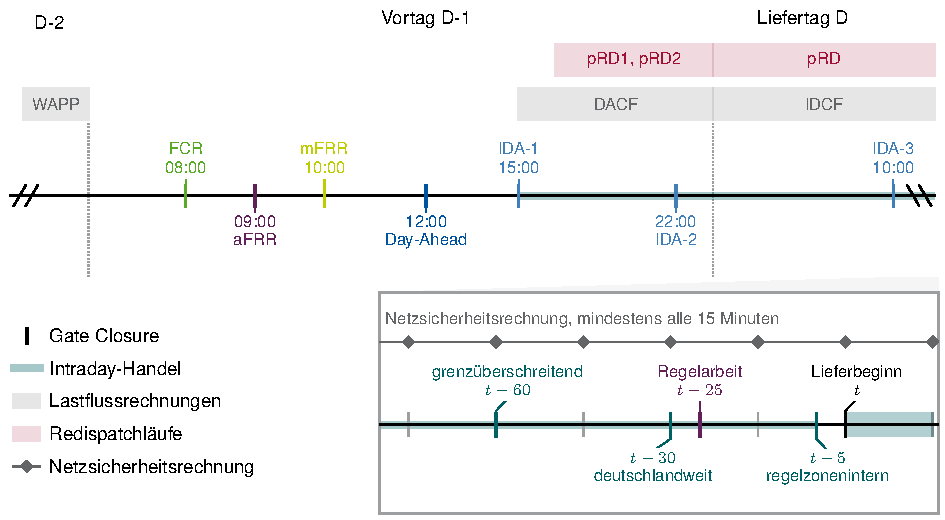
\includegraphics[width=\textwidth]{figures/chapter_2/markt_zeitschiene.pdf}
    \caption{Zeitliche Staffelung der Handelsgelegenheiten, der Beschaffung von Systemdienstleistungen und der Rechenläufe des \ac{ÜNB} bis zum Erfüllungszeitpunkt.}
    \label{fig:markt_zeitschiene}
\end{figure}

% NEUER ABSATZ am 20.09.2026. UMBAU am 20.09.2026, Vorgabe des Verfassers: "ich wollte im Kapitel 2.2.1 die Zeitschienen haben ... fuege die Zeitschienen fuer Regelleistung und Redispatch in 2.2.1 ein und versuche, so wenig wie moeglich darauf in 2.2.2 einzugehen. 2.2.2 soll eher erklaeren, was dort gemacht wird, wie der Rahmen ist, wofuer und wer daran teilnimmt, aber so wenig wie moeglich Verguetung."
% Die drei Saetze standen bis heute in 2.2.2. Handelsschluss nach regelleistung.net (lokal nur die FCR bei
% Consentec 2026 belegt), Regelarbeitsmarkt nach dem Monitoringbericht 2025. Die Akronyme FCR, aFRR und mFRR
% werden hier erstmals aufgeloest, einen Absatz vor ihrer Erklaerung in 2.2.2, Preis der Reihenfolge.
Vor den Energiemärkten schließen am Vortag die Ausschreibungen der Regelleistung, nämlich um 8 Uhr für die \ac{FCR}, um 9 Uhr für die \ac{aFRR} und um 10 Uhr für die \ac{mFRR} \cite{regelleistung_ausschreibungsdaten_2026}.
Der Regelarbeitsmarkt für die \ac{aFRR} und die \ac{mFRR} öffnet nach der Verkündung der Zuschläge und schließt 25 Minuten vor Beginn der jeweiligen Viertelstunde \cite{bundesnetzagentur_monitoringbericht_2026}.
Ein Anbieter plant seine Vermarktung an den Energiemärkten deshalb bereits unter Berücksichtigung eines vom \ac{ÜNB} erteilten Zuschlags.

% NEUER ABSATZ 16.09.2026, C2.8.
% R-34 am 18.09.2026, Kontrolle durch Fable, Entscheidung des Verfassers: Satz geteilt, Stilregel 17. Alte Fassung:
%Den Ausgangspunkt der betrachteten Fahrplanbildung bildet daher der \ac{DA}, dessen Auktion um 12 Uhr des Vortages schließt und alle Lieferzeitpunkte des Folgetages in einem Auktionsdurchgang zum einheitlichen Markträumungspreis preist, seit dem 1.\,Oktober 2025 in Viertelstundenprodukten.
% UMBAU am 20.09.2026, Vorgabe des Verfassers: "ich wollte im Kapitel 2.2.1 die Zeitschienen haben ... fuege die Zeitschienen fuer Regelleistung und Redispatch in 2.2.1 ein und versuche, so wenig wie moeglich darauf in 2.2.2 einzugehen. 2.2.2 soll eher erklaeren, was dort gemacht wird, wie der Rahmen ist, wofuer und wer daran teilnimmt, aber so wenig wie moeglich Verguetung."
% Das daher bezog sich auf Terminmarkt und OTC, dazwischen steht jetzt die Regelleistung. Alte Fassung:
%Den Ausgangspunkt der betrachteten Fahrplanbildung bildet daher der \ac{DA}, dessen Auktion um 12 Uhr des Vortages schließt.
Den Ausgangspunkt der betrachteten Fahrplanbildung an den Energiemärkten bildet der \ac{DA}, dessen Auktion um 12 Uhr des Vortages schließt.
% BELEG ERGAENZT am 19.09.2026, Befund der Zahlenpruefung: der Termin stand ohne Zitat, und der
% naechste Beleg im Absatz ist mahgoub_wie_2025, dem er dadurch faelschlich zugerechnet wuerde.
% mahgoub_wie_2025 stammt von Februar 2025 und nennt noch den damals geplanten Termin: "Im Juni
% 2025 steht mit der Umstellung der Day-Ahead (DA) Auktion von Stunden- auf Viertelstundenprodukte
% eine weitere bedeutende Marktdesign-Veraenderung an." Der Termin wurde spaeter verschoben.
% ffe_saegezahn_2026 traegt ihn: "Zum 01.10.2025 wurden die europaeischen Day-Ahead (DA)-Maerkte
% auf 15-Minuten-Handelsprodukte umgestellt." Die Quelle steht im selben Absatz noch einmal beim
% Satz zur Verlagerung des kurzfristigen Ausgleichs; die zweite Nennung ist bewusst in Kauf
% genommen, weil der Beleg sonst hinter mahgoub_wie_2025 zu stehen kaeme, Stilregel 15. Alte
% Fassung:
%Die Auktion preist alle Lieferzeitpunkte des Folgetages in einem Durchgang zum einheitlichen Markträumungspreis, seit dem 1.\,Oktober 2025 in Viertelstundenprodukten.
% GEAENDERT am 20.09.2026, Wortlaut des Verfassers: "bis zum 1. oktober als stundenprodukt
% und seitdem als viertelstunden produkt". Der alte Produktschnitt stand nicht im Satz. Alte Fassung:
%Die Auktion preist alle Lieferzeitpunkte des Folgetages in einem Durchgang zum einheitlichen Markträumungspreis, seit dem 1.\,Oktober 2025 in Viertelstundenprodukten \cite{ffe_saegezahn_2026}.
Die Auktion preist alle Lieferzeitpunkte des Folgetages in einem Durchgang zum einheitlichen Markträumungspreis, bis zum 1.\,Oktober 2025 in Stundenprodukten und seitdem in Viertelstundenprodukten \cite{ffe_saegezahn_2026}.
% R-34 am 18.09.2026, Kontrolle durch Fable, Entscheidung des Verfassers: Satz geteilt, Stilregel 17. Alte Fassung:
%Daran schließen die seit Juni 2024 etablierten Intraday-Auktionen an, die den Fahrplan zu definierten Zeitpunkten gegen aktualisierte Prognosen neu bewerten \cite{mahgoub_wie_2025}: Die \ac{IDA-1} schließt um 15 Uhr und die \ac{IDA-2} um 22 Uhr des Vortages, beide mit dem gesamten Folgetag als Handelsfenster, während die \ac{IDA-3} um 10 Uhr des Liefertages schließt und nur noch dessen zweite Hälfte umfasst.
% PRAEZISIERT am 19.09.2026, Befund der Zahlenpruefung: die IDA-1 bestand vor dem 13.06.2024 als
% einzige Viertelstunden-Intraday-Auktion, neu sind seither die europaweite Vereinheitlichung im
% SIDC und die beiden Auktionen IDA-2 und IDA-3. Monitoringbericht, S. 142: "Am 13. Juni 2024
% wurde ... die 15-Minuten Intraday Auktion fuer das deutsche Marktgebiet durch drei Intraday
% Auktionen (IDAs) ersetzt." Alte Fassung:
%Daran schließen die seit Juni 2024 etablierten Intraday-Auktionen an, die den Fahrplan zu definierten Zeitpunkten gegen aktualisierte Prognosen neu bewerten \cite{mahgoub_wie_2025}.
% BELEG VERSCHOBEN am 20.09.2026: mahgoub_wie_2025 steht jetzt beim neuen Satz zum Viertelstundenausgleich,
% damit die Quelle im Absatz nur einmal steht, Stilregel 15. Alte Fassung:
%Daran schließen die Intraday-Auktionen an, die den Fahrplan zu definierten Zeitpunkten gegen aktualisierte Prognosen neu bewerten \cite{mahgoub_wie_2025}.
Daran schließen die Intraday-Auktionen an, die den Fahrplan zu definierten Zeitpunkten gegen aktualisierte Prognosen neu bewerten.
Seit dem 13.\,Juni 2024 finden drei Intraday-Auktionen statt, zuvor war es eine einzige.
Die \ac{IDA-1} schließt um 15 Uhr und die \ac{IDA-2} um 22 Uhr des Vortages, beide mit dem gesamten Folgetag als Handelsfenster.
Die \ac{IDA-3} schließt um 10 Uhr des Liefertages und umfasst nur noch dessen zweite Hälfte.
% ERGAENZT am 20.09.2026, Kommentar des Verfassers: "kurz erklaeren, dass auch durch 15-min-Handelsfenster viel
% dort gehandelt wurde, deswegen konnte dieser Shift zurueck durch die DA-Aenderung ueberhaupt passieren".
% mahgoub_wie_2025: "Waehrend auf dem DA-Markt aktuell noch Produkte mit einer minimalen zeitlichen
% Granularitaet von einer Stunde gehandelt werden, koennen auf den Intraday-Maerkten Viertelstundenprodukte
% gehandelt werden. Dementsprechend werden auf dem Intraday-Markt auch Abweichungen des erwarteten
% Preisniveaus fuer jede Viertelstunde im Vergleich zum Stundenwert ausgeglichen." Ein Mengenwort traegt
% die Quelle nicht, sie beziffert die drei Auktionen auf rund 3 Prozent des Spotvolumens, deshalb ohne viel.
Die Intraday-Auktionen handeln Viertelstundenprodukte.
Solange der \ac{DA} nur Stundenprodukte kannte, glichen die \ac{EIV} dort die Abweichung ihres Viertelstundenprofils vom Stundenwert aus \cite{mahgoub_wie_2025}.
% ANGEBUNDEN am 20.09.2026 an die zwei neuen Vorsaetze, Bezug ausgeschrieben. Alte Fassung:
%Mit der Umstellung des Produktschnitts hat sich ein Teil des kurzfristigen Ausgleichs aus diesen Auktionen in die Auktion des \ac{DA} verlagert, weil die Viertelstundenprodukte dort nun selbst gehandelt werden \cite{ffe_saegezahn_2026}.
Mit der Umstellung des Produktschnitts hat sich dieser Ausgleich zum Teil aus den Intraday-Auktionen in die Auktion des \ac{DA} verlagert, weil die Viertelstundenprodukte dort nun selbst gehandelt werden \cite{ffe_saegezahn_2026}.
% I-39 am 18.09.2026, Kontrolle durch Fable, Entscheidung des Verfassers: die Handelsschlusszeiten standen ohne Quelle. EPEX war nicht im Wortlaut pruefbar, SMARD traegt alle drei Zeiten. Alte Fassung:
%Den Abschluss bildet der \ac{IDC}, der mit der ersten Intraday-Auktion einsetzt, jedes Geschäft zum zwischen den Parteien vereinbarten Preis abrechnet und die Anpassung bis zum Handelsschluss offenhält, der gestaffelt eintritt, nämlich 60 Minuten vor Lieferbeginn für den grenzüberschreitenden Handel, 30 Minuten davor für den Handel zwischen den Regelzonen und 5 Minuten davor für den regelzoneninternen Handel.
% PRAEZISIERT UND GETEILT am 19.09.2026, Befund der Zahlenpruefung. Erstens war die Wendung
% "30 Minuten davor" und "5 Minuten davor" mehrdeutig, weil davor sich grammatisch auch auf die
% zuvor genannten 60 Minuten beziehen liesse; alle drei Fristen beziehen sich auf den
% Lieferbeginn. Zweitens gelten die 30 und die 5 Minuten fuer die EPEX SPOT; der
% Monitoringbericht nennt auf S. 141 fuer die Nord Pool 20 Minuten beziehungsweise den Handel
% bis zum Lieferzeitpunkt. Die 60 Minuten sind dagegen der Schluss des gebotszonenuebergreifenden
% Intraday-Marktes im SIDC und gelten allgemein. Drittens ist der Satz nach Stilregel 17 geteilt.
% Alte Fassung:
%Den Abschluss bildet der \ac{IDC}, der mit der ersten Intraday-Auktion einsetzt, jedes Geschäft zum zwischen den Parteien vereinbarten Preis abrechnet und die Anpassung bis zum Handelsschluss offenhält, der gestaffelt eintritt, nämlich 60 Minuten vor Lieferbeginn für den grenzüberschreitenden Handel, 30 Minuten davor für den Handel zwischen den Regelzonen und 5 Minuten davor für den regelzoneninternen Handel \cite{bundesnetzagentur_smard_grosshandelspreise_2026}.
Den Abschluss bildet der \ac{IDC}, der mit der ersten Intraday-Auktion einsetzt, jedes Geschäft zum zwischen den Parteien vereinbarten Preis abrechnet und die Anpassung bis zum Handelsschluss offenhält.
Der Handelsschluss tritt gestaffelt ein, nämlich 60 Minuten vor Lieferbeginn für den grenzüberschreitenden Handel und an der EPEX SPOT 30 Minuten für den Handel zwischen den Regelzonen und 5 Minuten für den regelzoneninternen Handel \cite{bundesnetzagentur_smard_grosshandelspreise_2026}.
Das Preisniveau des \ac{IDC} bilden der \ac{ID3} und der \ac{ID1} ab, die beide volumengewichtet sind.

% NEU GEFASST am 15.09.2026 nach dem Absatzplan im Sammelmodus.
% Befunde G31, Q2, Q14. Sechs Saetze auf drei.
% Alte Fassung, nicht wieder aufnehmen:
%Über den Handelsgelegenheiten liegen die Rechenläufe des \ac{ÜNB}, die den Netzzustand aus den gemeldeten Fahrplänen ableiten.
%Die zugrunde liegenden Lastflussberechnungen sind europäisch koordiniert, denn die \ac{ÜNB} tauschen ihre Fahrplan- und Netzdaten dafür untereinander aus.
%Am Vortag wird der \ac{DACF} für den gesamten Folgetag gerechnet, während am Liefertag der \ac{IDCF} untertägig folgt \cite{leeuwen_integration_2020}.
%Auf diesen Berechnungen setzen die präventiven Redispatch-Prozesse auf.
%Die Netzsicherheitsrechnung wird daraus ausgelöst und prüft für jede folgende Viertelstunde, ob der \mbox{(N-1)-sichere} Zustand gewahrt bleibt.
%Zwischen dem letzten vorausschauenden Rechenlauf und dem Lieferbeginn bleibt gleichwohl ein Handelsfenster offen, in dem der Fahrplan noch verändert werden darf, ohne dass die Meldung dieser Änderung noch in einen der genannten Rechenläufe eingeht.
% R-35 am 18.09.2026, Kontrolle durch Fable, Entscheidung des Verfassers: Satz geteilt, Stilregel 17. Alte Fassung:
%Über den Handelsgelegenheiten liegen die Rechenläufe des \ac{ÜNB}, die den Netzzustand aus den gemeldeten Fahrplänen ableiten und europäisch koordiniert sind, weil die \ac{ÜNB} ihre Fahrplan- und Netzdaten dafür austauschen: Am Vortag wird der \ac{DACF} für den gesamten Folgetag gerechnet, am Liefertag folgt untertägig der \ac{IDCF} \cite{leeuwen_integration_2020}.
Über den Handelsgelegenheiten liegen die Rechenläufe des \ac{ÜNB}, die den Netzzustand aus den gemeldeten Fahrplänen ableiten.
Die Rechenläufe sind europäisch koordiniert, weil die \ac{ÜNB} ihre Fahrplan- und Netzdaten dafür austauschen.
Am Vortag rechnen die \ac{ÜNB} den \ac{DACF} für den gesamten Folgetag, am Liefertag folgt untertägig der \ac{IDCF} \cite{leeuwen_integration_2020}.
% SATZLAENGE am 15.09.2026, Stilregel 17, alte Fassung als Kommentar:
%Auf diesen Berechnungen setzen die präventiven Redispatch-Prozesse auf, und die Netzsicherheitsrechnung prüft kontinuierlich, ob der \mbox{(N-1)-sichere} Zustand gewahrt bleibt, denn an einen abgeschlossenen Rechenlauf schließt sich unmittelbar der nächste an.
Auf diesen Berechnungen setzen die präventiven Redispatch-Prozesse auf.
% HIERHER VERSCHOBEN am 20.09.2026 aus 2.2.2. UMBAU am 20.09.2026, Vorgabe des Verfassers: "ich wollte im Kapitel 2.2.1 die Zeitschienen haben ... fuege die Zeitschienen fuer Regelleistung und Redispatch in 2.2.1 ein und versuche, so wenig wie moeglich darauf in 2.2.2 einzugehen. 2.2.2 soll eher erklaeren, was dort gemacht wird, wie der Rahmen ist, wofuer und wer daran teilnimmt, aber so wenig wie moeglich Verguetung."
% Leeuwen ist im Absatz bereits beim DACF-Satz zitiert, deshalb ohne zweiten Beleg, Stilregel 15. Aufforderung
% zu Anordnung, weil Paragraph 13a erst in 2.2.2 eingefuehrt wird.
Jeder dieser Prozesse rechnet den prognostizierten Netzzustand mit einem Lastflussmodell durch und bestimmt daraus Engpässe und Maßnahmen.
Am Vortag dient der Prozess pRD1 gegen 16:30 Uhr der Sicherung von Redispatchpotenzialen durch Kraftwerksanfahrten, die einen langen Vorlauf brauchen.
Gegen 18 Uhr bestimmt pRD2 auf dem \ac{DACF} die Arbeitspunktanpassungen für den Liefertag.
Am Liefertag folgen auf dem rollierenden \ac{IDCF} weitere präventive Redispatchläufe.
Eine Anordnung zum Redispatch trifft damit einen Fahrplan, der am \ac{DA} und in der \ac{IDA-1} bereits vermarktet ist, und untertägig oder aus der Netzsicherheitsrechnung heraus einen Fahrplan im laufenden \ac{IDC}.
% DURCHSICHT 16.09.2026, C1. Alte Fassung:
%Die Netzsicherheitsrechnung prüft kontinuierlich, ob der \mbox{(N-1)-sichere} Zustand gewahrt bleibt.
% ATTRIBUT am 20.09.2026, Kommentar des Verfassers: "Netzsicherheitsrechnung anhand von Messdaten und State
% Estimation aus den realen Fluessen, pruefe auf Dopplung". Die State Estimation ist in 2.1.2 erklaert
% ("also der aus Messwerten geschaetzten Netzsituation"), hier steht deshalb nur das Attribut ohne
% erneute Definition, Stilregel 6. Alte Fassung:
%Die Netzsicherheitsrechnung prüft darüber hinaus kontinuierlich, ob der \mbox{(N-1)-sichere} Zustand gewahrt bleibt.
Die Netzsicherheitsrechnung prüft darüber hinaus kontinuierlich anhand der aus Messwerten geschätzten Netzsituation, ob der \mbox{(N-1)-sichere} Zustand gewahrt bleibt.
% S-08 am 18.09.2026, Kontrolle durch Fable, Entscheidung des Verfassers: gestrichen, die Aussage traegt der vorige Satz mit kontinuierlich. Gestrichener Satz: Alte Fassung:
%An einen abgeschlossenen Rechenlauf schließt sich dabei unmittelbar der nächste an.
% S-08 am 18.09.2026, Kontrolle durch Fable, Entscheidung des Verfassers: Satz gekuerzt, die Luecke steht in 1.1 und 2.1.1. Alte Fassung:
%Zwischen dem letzten vorausschauenden Rechenlauf und dem Lieferbeginn bleibt gleichwohl das Handelsfenster offen, in dem der Fahrplan noch verändert werden darf, ohne dass die Änderung in einen der genannten Rechenläufe eingeht, sodass der \ac{ÜNB} solche Änderungen erst in der laufenden Netzsicherheitsrechnung sieht.
% ZU ENDE GEFUEHRT am 20.09.2026, Kommentar des Verfassers: "im Worst Case sieht er auch in laufenden
% Netzsicherheitsrechnungen Aenderungen des Fahrplans nicht mehr, was zu einer N-1-Verletzung fuehren kann,
% weiss aber nicht, ob wir die Aussage hier platzieren wollen". Umgesetzt als Folgesatz mit Verweis auf
% 2.1.1, wo die Folge bereits steht ("nur noch mit Mitteln ohne Vorlauf beheben"). Der Ausdruck
% N-1-Verletzung ist nicht uebernommen, Stilregel 9, das Netz wird N-1-sicher betrieben. Alte Fassung:
%Änderungen des Fahrplans nach dem letzten vorausschauenden Rechenlauf sieht der \ac{ÜNB} deshalb erst in der laufenden Netzsicherheitsrechnung.
Änderungen des Fahrplans nach dem letzten vorausschauenden Rechenlauf sieht der \ac{ÜNB} deshalb erst, wenn sie sich in den Messwerten zeigen.
Für eine Maßnahme mit Vorlauf bleibt dann keine Zeit mehr, wie in Abschnitt~\ref{sec:prev_vs_cur} beschrieben.

\subsection{Systemdienstleistungen}
\label{sec:ancillary_services}
% NEU GEFASST am 15.09.2026 nach dem Absatzplan im Sammelmodus.
% Befunde G32, Stilregel 5. Spannungshaltung und Versorgungswiederaufbau in einem Satz, Beschaffungslogik in den ersten Satz gezogen.
% Alte Fassung, nicht wieder aufnehmen:
%Die Systemdienstleistungen der Übertragungsnetzbetreiber gliedern sich üblicherweise in Frequenzhaltung, Spannungshaltung, Betriebsführung und Versorgungswiederaufbau.
%Die Spannungshaltung wird über Blindleistung erbracht und berührt die Wirkleistungseinspeisung nicht unmittelbar.
%Der Versorgungswiederaufbau setzt zwar Wirkleistung ein, beruht aber auf der Schwarzstartfähigkeit einzelner Anlagen und nicht auf der an den Energiemärkten gehandelten Wirkleistung.
%Beide konkurrieren damit nicht mit der Vermarktung an den Energiemärkten.
%In der Frequenzhaltung wird demgegenüber ein Band an Wirkleistung über einen Zeitraum reserviert und die Bereitstellung selbst vergütet, weshalb sie das einzige Regime ist, in dem eine Vorhaltung bereits einen Preis hat \cite{ubertragungsnetzbetreiber_deutschland_praqualifikationsverfahren_2024}.
%Auch die Betriebsführung greift auf die Wirkleistung zu, und zu ihr zählen das Engpassmanagement und die kurative Vorhaltung.

%Die Frequenzhaltung wird in Deutschland über drei Regelleistungsprodukte beschafft, nämlich die \ac{FCR}, die \ac{aFRR} und die \ac{mFRR}.
%Ihre Beschaffung folgt einer ähnlichen, aber nicht in allen Punkten gleichen Logik.
%Die \ac{ÜNB} schreiben eine Leistungsmenge aus, die Anbieter geben Leistungspreise ab, und die Zuschlagserteilung verpflichtet den Anbieter, die zugesagte Leistung über die gesamte Erbringungsperiode bereitzuhalten \cite{ubertragungsnetzbetreiber_deutschland_praqualifikationsverfahren_2024}.
%Voraussetzung für die Teilnahme ist ein Präqualifikationsverfahren, in dem die technische Eignung der Anlage nachgewiesen und ein zulässiger Arbeitsbereich festgelegt wird.
%Bei der \ac{aFRR} und der \ac{mFRR} werden Leistung und Arbeit in zwei getrennten Ausschreibungen beschafft, während bei der \ac{FCR} allein Leistung beschafft wird.
%Die beschaffte Menge folgt dabei zwei verschiedenen Regeln.
%Der Bedarf an \ac{FCR} wird auf europäischer Ebene festgelegt und geht vom Ausfall einer Erzeugungsleistung von 3000\,\si{MW} als Referenzstörfall aus, der über einen jährlich neu berechneten Schlüssel auf die Regelzonen verteilt wird, woraus für Deutschland im Jahr 2024 eine Ausschreibung von 564\,\si{MW} folgte \cite{bundesnetzagentur_monitoringbericht_2026}.
%Den Bedarf an \ac{aFRR} und \ac{mFRR} ermitteln die deutschen \ac{ÜNB} dagegen gemeinsam und schreiben ihn je Vier-Stunden-Zeitscheibe aus, sodass sich die Menge über den Tag ändert.
%Tabelle~\ref{tab:regelleistung} stellt die Produktmerkmale gegenüber.
% SATZLAENGE am 15.09.2026, Vorgabe des Verfassers, Hauptsatz und hoechstens ein Nebensatz.
% R-36 am 18.09.2026, Kontrolle durch Fable, Entscheidung des Verfassers: These nach vorn, Stilregel 1. Alte Fassung:
%Neben den Energiemärkten beschaffen die \ac{ÜNB} Systemdienstleistungen.
% BERICHTIGT am 20.09.2026, Kommentar des Verfassers: "das stimmt nicht. Schwarzstartfaehigkeit wird auch
% marktlich beschafft, jedoch sind die Regelleistungsmaerkte durch Wirkleistungslieferungen auch mit den
% Spotmaerkten verbunden, Schwarzstartfaehigkeit beschafft ja eine reine Faehigkeit. Ich will das aber
% nicht zu gross aufmachen." Monitoringbericht 2025, S. 118: "Schwarzstartfaehigkeit bezeichnet die
% Faehigkeit eines Kraftwerks, nach einem vollstaendigen Stromausfall eigenstaendig wieder hochzufahren",
% "marktgestuetzte Beschaffung dieser nichtfrequenzgebundenen Systemdienstleistung", "Basierend auf
% Paragraph 12h Abs. 1 Nr. 5 EnWG verpflichtet die Festlegung [BK6-21-023] die Uebertragungsnetzbetreiber,
% die Schwarzstartfaehigkeit ... zu beschaffen." Alte Fassung:
%Die Frequenzhaltung ist das einzige Regime, in dem eine Vorhaltung bereits einen Preis hat.
% NEU GEFASST am 20.09.2026 nach dem Absatzplan, freigegeben vom Verfasser ("alle drei abhaken").
% Kommentar: "Schwarzstartfaehigkeit und Blindleistung sind fuer Speicher schon relevant, da sie fuer
% Schwarzstartfaehigkeit auch einen Energieinhalt benoetigen bzw. fuer Blindleistung Energie aus dem SOC.
% Ich wuerde deswegen vorsichtiger formulieren und eher in die Richtung, dass Frequenzhaltung schon
% marktlich aehnlich ausgestaltet ist ... der Fokus sollte klar auf den Regelleistungsmaerkten sein, da
% die ja auch nachweislich sehr konkurrieren." Reihenfolge: Gliederung, These Frequenzhaltung,
% Betriebsfuehrung, Blindleistung und Schwarzstart mit Ladezustand, Frequenzhaltung als das der
% kurativen Vorhaltung in der Form naechste Regime. "Erst anlaeuft" traegt der Monitoringbericht:
% erstmals zwoelf Monate nach der Festlegung vom Juni 2024 in einer Beschaffungsregion, binnen 36
% Monaten in allen. Kein Verweis auf 2.3.5 im Thesensatz, Entscheidung durch Fable, weil der Satz sonst
% zwei "wie" truege. Alte Fassung, nicht wieder aufnehmen:
%Die Frequenzhaltung ist das einzige Regime mit einem Preis für die Vorhaltung von Wirkleistung, die sonst an den Energiemärkten vermarktet würde.
%Neben den Energiemärkten beschaffen die \ac{ÜNB} Systemdienstleistungen.
%Die Systemdienstleistungen gliedern sich üblicherweise in Frequenzhaltung, Spannungshaltung, Betriebsführung und Versorgungswiederaufbau.
%Die Spannungshaltung wird über Blindleistung erbracht, und der Versorgungswiederaufbau beruht auf der Schwarzstartfähigkeit einzelner Anlagen.
%Die \ac{ÜNB} beschaffen auch Blindleistung und Schwarzstartfähigkeit nach §\,12h \ac{EnWG} marktgestützt und vergüten damit eine Vorhaltung, die aber keine Wirkleistung bindet \cite{bundesnetzagentur_monitoringbericht_2026}.
%Spannungshaltung und Versorgungswiederaufbau konkurrieren deshalb nicht mit der Vermarktung von Wirkleistung an den Energiemärkten.
%In der Frequenzhaltung wird demgegenüber ein Band an Wirkleistung über einen Zeitraum reserviert, und die Bereitstellung selbst wird vergütet \cite{ubertragungsnetzbetreiber_deutschland_praqualifikationsverfahren_2024}.
%Auch die Betriebsführung greift auf die Wirkleistung zu, und zu ihr zählen das Engpassmanagement und die kurative Vorhaltung.
% ERGAENZT am 20.09.2026, siehe Vermerk am Absatzanfang.
% ERWEITERT am 20.09.2026, Rueckfrage des Verfassers: "wird Blindleistungserbringung nicht auch
% marktgestuetzt beschafft?" Ja: Paragraph 12h Abs. 1 Nr. 1 EnWG "Dienstleistungen zur Spannungsregelung",
% Monitoringbericht 2025: "Die Bundesnetzagentur hat am 25. Juni 2024 eine Festlegung zur marktbasierten
% Beschaffung von Blindleistung ... Standardprodukte ... Anbieterauswahl und Verguetung". Alte Fassung:
%Die \ac{ÜNB} beschaffen die Schwarzstartfähigkeit nach §\,12h \ac{EnWG} zwar marktgestützt und vergüten damit ebenfalls eine Vorhaltung, beschafft wird aber eine Fähigkeit der Anlage und keine Wirkleistung \cite{bundesnetzagentur_monitoringbericht_2026}.
% BEZUG AUSGESCHRIEBEN am 20.09.2026, weil der neue Satz dazwischen steht, Stilregel 5. Alte Fassung:
%Beide konkurrieren deshalb nicht mit der Vermarktung von Wirkleistung an den Energiemärkten.
% HIERHER VERSCHOBEN 16.09.2026, C1, vor die Konsequenz.
Neben den Energiemärkten beschaffen die \ac{ÜNB} Systemdienstleistungen, die sich üblicherweise in Frequenzhaltung, Spannungshaltung, Betriebsführung und Versorgungswiederaufbau gliedern.
Für die Fahrplanbildung eines \ac{BESS} ist davon die Frequenzhaltung maßgeblich, weil sie dasselbe Wirkleistungsband beansprucht wie die Vermarktung an den Energiemärkten.
Auch die Betriebsführung greift auf die Wirkleistung zu, und zu ihr zählen das Engpassmanagement und die kurative Vorhaltung.
Die Spannungshaltung wird über Blindleistung erbracht, und der Versorgungswiederaufbau beruht auf der Schwarzstartfähigkeit einzelner Anlagen.
Die \ac{ÜNB} beschaffen Blindleistung und Schwarzstartfähigkeit nach §\,12h \ac{EnWG} marktgestützt und vergüten damit ebenfalls eine Vorhaltung \cite{bundesnetzagentur_monitoringbericht_2026}.
Für ein \ac{BESS} können Blindleistung und Schwarzstartfähigkeit einen Teil des Ladezustands beanspruchen.
Beide Dienstleistungen bleiben im Weiteren dennoch außer Betracht, weil ihre marktgestützte Beschaffung erst anläuft und das Leistungsband des \ac{BESS} nicht bindet.
In der Frequenzhaltung wird dagegen ein Band an Wirkleistung über einen Zeitraum reserviert, und die Bereitstellung selbst wird vergütet \cite{ubertragungsnetzbetreiber_deutschland_praqualifikationsverfahren_2024}.
Die Frequenzhaltung ist damit das Regime, dessen Beschaffung der kurativen Vorhaltung in der Form am nächsten kommt.
% R-36 am 18.09.2026, Kontrolle durch Fable, Entscheidung des Verfassers: der Satz traegt die Kernaussage und steht jetzt am Anfang des Absatzes. Alte Fassung:
%Die Frequenzhaltung ist damit das einzige Regime, in dem eine Vorhaltung bereits einen Preis hat.
% VERSCHOBEN 16.09.2026, C1, vor die Konsequenz: Auch die Betriebsführung greift auf die Wirkleistung zu, und zu ihr zählen das Engpassmanagement und die kurative Vorhaltung.

Die Frequenzhaltung wird in Deutschland über drei Regelleistungsprodukte beschafft, nämlich die \ac{FCR}, die \ac{aFRR} und die \ac{mFRR}.
% S-20 am 18.09.2026, Kontrolle durch Fable, Entscheidung des Verfassers: gestrichen, die folgenden Saetze zeigen Gemeinsamkeiten und Unterschiede selbst. Gestrichener Satz: Alte Fassung:
%Die Beschaffung folgt einer ähnlichen, aber nicht in allen Punkten gleichen Logik.
Die \ac{ÜNB} schreiben eine Leistungsmenge aus, und die Anbieter geben Leistungspreise ab.
Der Zuschlag verpflichtet den Anbieter, die zugesagte Leistung über die gesamte Erbringungsperiode bereitzuhalten \cite{ubertragungsnetzbetreiber_deutschland_praqualifikationsverfahren_2024}.
Voraussetzung für die Teilnahme ist ein Präqualifikationsverfahren, in dem die technische Eignung der Anlage nachgewiesen und ein zulässiger Arbeitsbereich festgelegt wird.
% ERGAENZT am 20.09.2026. UMBAU am 20.09.2026, Vorgabe des Verfassers: "ich wollte im Kapitel 2.2.1 die Zeitschienen haben ... fuege die Zeitschienen fuer Regelleistung und Redispatch in 2.2.1 ein und versuche, so wenig wie moeglich darauf in 2.2.2 einzugehen. 2.2.2 soll eher erklaeren, was dort gemacht wird, wie der Rahmen ist, wofuer und wer daran teilnimmt, aber so wenig wie moeglich Verguetung."
% PQ-Bedingungen 2024: "Die PQ-Leistung bzw. Vermarktbare Leistung eines Pools wird vom Anbieter als Aggregation
% der RE- und RG-Werte ... ", der Beleg steht im Satz davor, Stilregel 15.
Teilnehmen können präqualifizierte Anlagen jeder Technologie, einzeln oder als Pool.
Bei der \ac{aFRR} und der \ac{mFRR} werden Leistung und Arbeit in zwei getrennten Ausschreibungen beschafft, während bei der \ac{FCR} allein Leistung beschafft wird.
% HIERHER VERSCHOBEN 16.09.2026, C2, Produktmerkmale zur Beschaffungslogik.
Die \ac{FCR} wird symmetrisch beschafft, die \ac{aFRR} und die \ac{mFRR} getrennt nach positiver und negativer Richtung.
% UMBAU am 20.09.2026, Vorgabe des Verfassers: "ich wollte im Kapitel 2.2.1 die Zeitschienen haben ... fuege die Zeitschienen fuer Regelleistung und Redispatch in 2.2.1 ein und versuche, so wenig wie moeglich darauf in 2.2.2 einzugehen. 2.2.2 soll eher erklaeren, was dort gemacht wird, wie der Rahmen ist, wofuer und wer daran teilnimmt, aber so wenig wie moeglich Verguetung."
% Verguetung, steht in 2.3.4 (Leistungspreis fuer die Vorhaltung, Arbeitspreis bei Abruf). Nicht wieder aufnehmen:
%Der Leistungspreis je Zeitscheibe steht mit dem Zuschlag fest, während der Arbeitspreis der \ac{aFRR} und der \ac{mFRR} je Viertelstunde und nur bei Abruf anfällt.
% HIERHER aus 2.3.4 am 20.09.2026. UMBAU am 20.09.2026, Vorgabe des Verfassers: "ich wollte im Kapitel 2.2.1 die Zeitschienen haben ... fuege die Zeitschienen fuer Regelleistung und Redispatch in 2.2.1 ein und versuche, so wenig wie moeglich darauf in 2.2.2 einzugehen. 2.2.2 soll eher erklaeren, was dort gemacht wird, wie der Rahmen ist, wofuer und wer daran teilnimmt, aber so wenig wie moeglich Verguetung."
% Monitoringbericht 2025: "Jeder Anbieter ist im Falle einer Bezuschlagung seines Gebotes auf dem RLM zu einer
% Angebotsabgabe verpflichtet". Der Monitoringbericht ist im Absatz damit zweimal zitiert (Mengen), in Kauf
% genommen wie am 19.09.2026.
Am Regelarbeitsmarkt kann jede präqualifizierte Einheit für jede Viertelstunde ein Arbeitsgebot abgeben, und wer einen Zuschlag für Leistung erhalten hat, ist dazu verpflichtet \cite{bundesnetzagentur_monitoringbericht_2026}.
Den Abruf löst bei der \ac{FCR} die örtliche Frequenzmessung aus, bei der \ac{aFRR} die europäische Plattform PICASSO und bei der \ac{mFRR} der \ac{ÜNB} von Hand über die Plattform MARI.
% ABSATZ VERBUNDEN am 20.09.2026, Vorgabe des Verfassers: Produkte, Mengen und Fristen der Regelleistung in einem Absatz.
Die beschaffte Menge folgt zwei verschiedenen Regeln.
% BELEG ERGAENZT am 19.09.2026, Befund der Zahlenpruefung: der Satz stand ohne Beleg. SO GL
% Art. 153 Abs. 2 lit. b traegt den Wert woertlich: "Fuer das Synchrongebiet Kontinentaleuropa
% beinhaltet der Referenzstoerfall 3 000 MW in positiver Richtung und 3 000 MW in negativer
% Richtung." Nach Art. 153 Abs. 2 lit. a muss die FCR-Kapazitaet den Referenzstoerfall mindestens
% abdecken, es ist also eine Mindestgroesse. Alte Fassung:
%Der Bedarf an \ac{FCR} wird auf europäischer Ebene festgelegt und geht vom Ausfall einer Erzeugungsleistung von 3000\,\si{MW} als Referenzstörfall aus.
% KOMPAKTER UND ERGAENZT am 20.09.2026, Kommentar des Verfassers: "da kann etwas kompakter geschrieben
% werden. Ich finde, die Leistungszahlen sind nicht sehr relevant, wenn wir sie nirgendwo anders als weder
% aFRR noch mFRR anfuehren. Deswegen streichen oder Zahlen ergaenzen." Ergaenzt, weil der
% Monitoringbericht 2025 alle Mengen traegt: "Im Jahr 2024 sank der Jahresdurchschnitt der
% ausgeschriebenen Primaerregelleistung leicht auf 564 MW", "positive Sekundaerregelleistung, deren
% durchschnittlich ausgeschriebene Leistung mit 1.941 MW", "negativen Sekundaerregelleistung betrug
% 1.817 MW", "positiver Minutenreserveleistung wurden durchschnittlich 603 MW ... und an negativer
% Minutenreserveleistung 364 MW ausgeschrieben". Der Verteilschluessel und das Wort Referenzstoerfall
% sind in einen Satz gezogen. Alte Fassung:
%Der Bedarf an \ac{FCR} wird auf europäischer Ebene festgelegt und geht vom Ausfall einer Erzeugungsleistung von 3000\,\si{MW} als Referenzstörfall aus \cite{europaische_kommission_verordnung_2017}.
%Ein jährlich neu berechneter Schlüssel verteilt diesen Bedarf auf die Regelzonen, woraus für Deutschland im Jahr 2024 eine im Jahresdurchschnitt ausgeschriebene Leistung von 564\,\si{MW} folgte \cite{bundesnetzagentur_monitoringbericht_2026}.
% BEZUGSGROESSE BERICHTIGT am 19.09.2026, Befund der Zahlenpruefung: die 564 MW sind der
% Jahresdurchschnitt der ausgeschriebenen Leistung und keine einzelne Ausschreibung.
% Monitoringbericht 2025, S. 22: "Im Jahr 2024 sank der Jahresdurchschnitt der ausgeschriebenen
% Primaerregelleistung leicht auf 564 MW (Vorjahr: 570 MW)." Alte Fassung:
%Ein jährlich neu berechneter Schlüssel verteilt diesen Bedarf auf die Regelzonen, woraus für Deutschland im Jahr 2024 eine Ausschreibung von 564\,\si{MW} folgte \cite{bundesnetzagentur_monitoringbericht_2026}.
Der Bedarf an \ac{FCR} wird auf europäischer Ebene aus dem Referenzstörfall von 3000\,\si{MW} abgeleitet und über einen jährlich neu berechneten Schlüssel auf die Regelzonen verteilt \cite{europaische_kommission_verordnung_2017}.
Den Bedarf an \ac{aFRR} und \ac{mFRR} ermitteln die deutschen \ac{ÜNB} gemeinsam und schreiben ihn je Vier-Stunden-Zeitscheibe aus, sodass sich die Menge über den Tag ändert.
Im Jahresdurchschnitt 2024 waren in Deutschland 564\,\si{MW} \ac{FCR} ausgeschrieben, 1941\,\si{MW} positive und 1817\,\si{MW} negative \ac{aFRR} sowie 603\,\si{MW} positive und 364\,\si{MW} negative \ac{mFRR} \cite{bundesnetzagentur_monitoringbericht_2026}.
% GEAENDERT am 15.09.2026, Tabelle 2.2 auf Vorgabe des Verfassers gestrichen, Inhalt in drei Saetzen. Alte Fassung:
%Tabelle~\ref{tab:regelleistung} stellt die Produktmerkmale und die Bemessung der Vergütung gegenüber.
% VERSCHOBEN 16.09.2026, C2, Produktmerkmale zur Beschaffungslogik: Die \ac{FCR} wird symmetrisch beschafft, die \ac{aFRR} und die \ac{mFRR} getrennt nach positiver und negativer Richtung.
% VERSCHOBEN 16.09.2026, C2, Produktmerkmale zur Beschaffungslogik: Der Leistungspreis je Zeitscheibe steht mit dem Zuschlag fest, während der Arbeitspreis der \ac{aFRR} und der \ac{mFRR} je Viertelstunde und nur bei Abruf anfällt.
% VERSCHOBEN 16.09.2026, C2, Produktmerkmale zur Beschaffungslogik: Den Abruf löst bei der \ac{FCR} die örtliche Frequenzmessung aus, bei der \ac{aFRR} die europäische Plattform PICASSO und bei der \ac{mFRR} der \ac{ÜNB} von Hand über die Plattform MARI.
% ABSATZ VERBUNDEN am 20.09.2026, Vorgabe des Verfassers: Produkte, Mengen und Fristen der Regelleistung in einem Absatz.
% TABELLE 2.2 GESTRICHEN am 15.09.2026 auf Vorgabe des Verfassers, Inhalt in drei Saetzen im Text. Alte Fassung, nicht wieder aufnehmen:
%\begin{table}[htbp]
%    \centering
% TABELLE ERWEITERT am 15.09.2026 um die Spalte Bemessung, Kuerzung A3, damit die Tabelle der Verguetungsbestandteile in 2.3.4 entfallen kann. Alte Fassung der Zeilen als Kommentar.
%    \caption{Produktmerkmale und Bemessung der drei Regelleistungsprodukte.}
%    \label{tab:regelleistung}
%    \small
%    \begin{tabular}{@{}>{\raggedright\arraybackslash}p{\dimexpr0.09\textwidth-\tabcolsep\relax}>{\raggedright\arraybackslash}p{\dimexpr0.20\textwidth-2\tabcolsep\relax}>{\raggedright\arraybackslash}p{\dimexpr0.28\textwidth-2\tabcolsep\relax}>{\raggedright\arraybackslash}p{\dimexpr0.26\textwidth-2\tabcolsep\relax}>{\raggedright\arraybackslash}p{\dimexpr0.17\textwidth-\tabcolsep\relax}@{}}
%    \begin{tabular}{@{}>{\raggedright\arraybackslash}p{\dimexpr0.08\textwidth-\tabcolsep\relax}>{\raggedright\arraybackslash}p{\dimexpr0.13\textwidth-2\tabcolsep\relax}>{\raggedright\arraybackslash}p{\dimexpr0.21\textwidth-2\tabcolsep\relax}>{\raggedright\arraybackslash}p{\dimexpr0.24\textwidth-2\tabcolsep\relax}>{\raggedright\arraybackslash}p{\dimexpr0.20\textwidth-2\tabcolsep\relax}>{\raggedright\arraybackslash}p{\dimexpr0.14\textwidth-\tabcolsep\relax}@{}}
%        \hline
%        \textbf{Produkt} & \textbf{Richtung} & \textbf{Produktschnitt} & \textbf{Aktivierung} & \textbf{Handelsschluss} \\
%        \textbf{Produkt} & \textbf{Richtung} & \textbf{Produktschnitt} & \textbf{Bemessung} & \textbf{Abruf} & \textbf{Handelsschluss} \\
%        \hline
%        \acs{FCR} & symmetrisch & Vier Stunden, nur Leistung & Automatisch, örtliche Frequenzmessung & 8 Uhr des Vortages \\
%        \acs{FCR} & symmetrisch & Vier Stunden, nur Leistung & Leistungspreis je Zeitscheibe, sicher & Automatisch, örtliche Frequenzmessung & 8 Uhr des Vortages \\
%        \hline
%        \acs{aFRR} & positiv und negativ & Vier Stunden, Leistung und Arbeit getrennt & Automatisch, Plattform PICASSO & 9 Uhr des Vortages \\
%        \acs{aFRR} & positiv und negativ & Vier Stunden, Leistung und Arbeit getrennt & Leistungspreis je Zeitscheibe, sicher, Arbeitspreis je Viertelstunde nur bei Abruf & Automatisch, Plattform PICASSO & 9 Uhr des Vortages \\
%        \hline
%        \acs{mFRR} & positiv und negativ & Vier Stunden, Leistung und Arbeit getrennt & Manuell, Plattform MARI & 10 Uhr des Vortages \\
%        \acs{mFRR} & positiv und negativ & Vier Stunden, Leistung und Arbeit getrennt & Leistungspreis je Zeitscheibe, sicher, Arbeitspreis je Viertelstunde nur bei Abruf & Manuell, Plattform MARI & 10 Uhr des Vortages \\
%        \hline
%        \multicolumn{5}{@{}p{\textwidth}@{}}{\footnotesize Der Handelsschluss bezieht sich auf die Ausschreibung der Leistung. Je Liefertag werden sechs Zeitscheiben ausgeschrieben.} \\
%        \multicolumn{6}{@{}p{\textwidth}@{}}{\footnotesize Der Handelsschluss bezieht sich auf die Ausschreibung der Leistung. Je Liefertag werden sechs Zeitscheiben ausgeschrieben. Der Arbeitspreis der \acs{aFRR} entsteht am Regelarbeitsmarkt mit Zuschlag 25 Minuten vor Beginn der Viertelstunde.} \\
%    \end{tabular}
%\end{table}
% ABSATZ VERBUNDEN am 20.09.2026, Vorgabe des Verfassers: Produkte, Mengen und Fristen der Regelleistung in einem Absatz.
% NEU GEFASST am 15.09.2026 nach dem Absatzplan im Sammelmodus.
% Befunde G33, Q8. Fuenf Saetze auf zwei, der Schlusssatz steht in 2.4.
% Alte Fassung, nicht wieder aufnehmen:
%Alle drei Ausschreibungen schließen nach Abbildung~\ref{fig:markt_zeitschiene} am Vortag und damit vor der Auktion des \ac{DA} ab, sodass ein Anbieter seine Vermarktung an den Energiemärkten bereits unter Berücksichtigung einer erteilten Zuschlagsverpflichtung plant.
%Wo eine Anlage im Netz steht, spielt für den Zuschlag keine Rolle, denn die Produkte dienen dem Frequenzausgleich in der gesamten Regelzone.
%Neben der Regelleistung ist das Engpassmanagement die zweite Systemdienstleistung, die auf die Wirkleistung zugreift.
%Es wird jedoch nicht marktlich beschafft, sondern angeordnet und auf Kostenbasis ausgeglichen.
%Die europäischen Vorgaben stellen dem Gesetzgeber dabei zwei Grundlagen der Preisfestsetzung zur Wahl, nämlich die an den Strommärkten geltenden Preise oder die transparent ermittelten Kosten der eingesetzten Ressourcen, und der deutsche Gesetzgeber hat sich für die Kosten entschieden \cite{europaische_kommission_verordnung_2015, bdew_branchenleitfaden_2018}.
%Der nicht marktbasierte Weg ist dabei nur unter Ausnahmetatbeständen zulässig, von denen für Deutschland zwei herangezogen werden, nämlich zu erwartendes strategisches und engpassverstärkendes Bietverhalten sowie ein Mangel an Wettbewerb im betroffenen Gebiet \cite{europaisches_parlament_und_rat_der_eu_verordnung_2019, hirth_kosten_2019}.
%Während die Regelleistung damit über Gebote bepreist wird, folgt die Vergütung im Engpassmanagement aus den Kosten der angeordneten Maßnahme.
% SATZLAENGE am 15.09.2026, Vorgabe des Verfassers, Hauptsatz und hoechstens ein Nebensatz.
% VERSCHOBEN am 15.09.2026 nach 2.3.4 auf Vorgabe des Verfassers, die Abgrenzung der mFRR steht dort. Wortlaut:
%Für ein \ac{BESS} sind von den drei Produkten die \ac{FCR} und die \ac{aFRR} von Belang, denn die \ac{mFRR} bietet bei gleichem Produktschnitt den geringeren Leistungspreis.
%Im Jahr 2025 lag der mittlere Leistungspreis der \ac{mFRR} nach eigener Auswertung der Ausschreibungsergebnisse bei 5 Euro je Megawatt und Stunde in positiver und 11 Euro je Megawatt und Stunde in negativer Richtung, der der \ac{aFRR} bei 18 Euro je Megawatt und Stunde und 16 Euro je Megawatt und Stunde \cite{regelleistung_ausschreibungsdaten_2026}.
%Der Erlösindex, der die Erlöse von \ac{BESS} am deutschen Markt ausweist, führt die \ac{mFRR} ebenfalls nicht \cite{isea_methodik_2026}.
%Die \ac{mFRR} bleibt deshalb im Weiteren außer Betracht.
% ZEITSCHIENE ERGAENZT am 20.09.2026, Kommentar des Verfassers: "im Abschnitt davor gehen wir bei
% Regelleistung auch kaum auf die Zeitschiene ein." Handelsschluss 8, 9 und 10 Uhr des Vortages wie in
% Abbildung 2.3 und in der am 15.09.2026 gestrichenen Tabelle 2.2; lokal traegt Consentec 2026 nur die
% FCR ("Gate Closure um 08:00 Uhr"), die drei Zeiten stehen auf regelleistung.net, Eintrag
% regelleistung_ausschreibungsdaten_2026, im Netz von Fable nicht pruefbar. Regelarbeitsmarkt nach dem
% Monitoringbericht 2025: "Der RAM oeffnet nach Verkuendung der RLM-Auktionsergebnisse und schliesst 25
% Minuten vor Beginn der jeweiligen Produktzeitscheibe." Der Monitoringbericht ist damit im Absatz zweimal
% zitiert, in Kauf genommen wie am 19.09.2026, weil beide Zahlen sonst ohne Beleg stuenden. Alte Fassung:
%Alle drei Ausschreibungen schließen nach Abbildung~\ref{fig:markt_zeitschiene} am Vortag und damit vor der Auktion des \ac{DA} ab.
% UMBAU am 20.09.2026, Vorgabe des Verfassers: "ich wollte im Kapitel 2.2.1 die Zeitschienen haben ... fuege die Zeitschienen fuer Regelleistung und Redispatch in 2.2.1 ein und versuche, so wenig wie moeglich darauf in 2.2.2 einzugehen. 2.2.2 soll eher erklaeren, was dort gemacht wird, wie der Rahmen ist, wofuer und wer daran teilnimmt, aber so wenig wie moeglich Verguetung."
% Nach 2.2.1 verschoben:
%Die Ausschreibungen der Leistung schließen nach Abbildung~\ref{fig:markt_zeitschiene} am Vortag um 8 Uhr für die \ac{FCR}, um 9 Uhr für die \ac{aFRR} und um 10 Uhr für die \ac{mFRR} und damit vor der Auktion des \ac{DA} \cite{regelleistung_ausschreibungsdaten_2026}.
% UMBAU am 20.09.2026, Vorgabe des Verfassers: "ich wollte im Kapitel 2.2.1 die Zeitschienen haben ... fuege die Zeitschienen fuer Regelleistung und Redispatch in 2.2.1 ein und versuche, so wenig wie moeglich darauf in 2.2.2 einzugehen. 2.2.2 soll eher erklaeren, was dort gemacht wird, wie der Rahmen ist, wofuer und wer daran teilnimmt, aber so wenig wie moeglich Verguetung."
% Nach 2.2.1 verschoben:
%Der Regelarbeitsmarkt für die \ac{aFRR} und die \ac{mFRR} öffnet nach der Verkündung der Zuschläge und schließt 25 Minuten vor Beginn der jeweiligen Viertelstunde \cite{bundesnetzagentur_monitoringbericht_2026}.
% AKTEUR ERGAENZT am 20.09.2026, Kommentar des Verfassers: "Zuschlagsverpflichtung des UeNB." Der UeNB
% erteilt den Zuschlag, die Verpflichtung traegt der Anbieter (Satz davor), deshalb "eines vom UeNB
% erteilten Zuschlags" statt "Zuschlagsverpflichtung des UeNB", Stilregel 12. Alte Fassung:
%Ein Anbieter plant seine Vermarktung an den Energiemärkten deshalb bereits unter Berücksichtigung einer erteilten Zuschlagsverpflichtung.
% UMBAU am 20.09.2026, Vorgabe des Verfassers: "ich wollte im Kapitel 2.2.1 die Zeitschienen haben ... fuege die Zeitschienen fuer Regelleistung und Redispatch in 2.2.1 ein und versuche, so wenig wie moeglich darauf in 2.2.2 einzugehen. 2.2.2 soll eher erklaeren, was dort gemacht wird, wie der Rahmen ist, wofuer und wer daran teilnimmt, aber so wenig wie moeglich Verguetung."
% Nach 2.2.1 verschoben:
%Ein Anbieter plant seine Vermarktung an den Energiemärkten deshalb bereits unter Berücksichtigung eines vom \ac{ÜNB} erteilten Zuschlags.
% DURCHSICHT 16.09.2026, C1. Alte Fassung:
%Wo eine Anlage im Netz steht, spielt für den Zuschlag keine Rolle, denn die Produkte dienen dem Frequenzausgleich in der gesamten Regelzone.
Wo eine Anlage im Netz steht, spielt für den Zuschlag zudem keine Rolle, denn die Produkte dienen dem Frequenzausgleich in der gesamten Regelzone.
% R-38 am 18.09.2026, Kontrolle durch Fable: der Absatz trug zwei Thesen, hier beginnt die zweite.

% NEU GEFASST am 20.09.2026, Kommentar des Verfassers: "schreib nicht, dass man sich zum kostenbasierten
% Redispatch entschieden hat, sondern dass es seit jeher so ist, man koennte fast sagen historisch
% gewachsen, aber einem Uebergang zu einer marktlichen Beschaffung stehen noch diese Vorbehalte gegenueber.
% Dazu erwaehnen, dass Redispatch, wie der Name schon sagt, den Dispatch korrigieren soll, eine marktliche
% Beschaffung den Dispatch aber zweiteilt und die marktlichen Akteure so die Moeglichkeit bekommen, das
% marktlich auszunutzen, wo eigentlich die Sicherheit des Netzes dahintersteht. Hier ist wieder die
% fehlende Netzsensitivitaet des Marktes." Belege, hirth_kosten_2019: "Das heutige System des Redispatch
% laesst sich als administrativer/regulatorischer Redispatch mit Kostenerstattung beschreiben", "Das
% Management von Netzengpaessen liegt ausserhalb der Marktsphaere ... Einher geht damit allerdings, dass
% der Markt keinerlei Anreize zur lokalen Steuerung setzt", "Die Koexistenz eines zonalen Strommarkts
% mit einem notwendigerweise lokalen Redispatch-Markt bietet Marktteilnehmern Anreize fuer strategisches
% Verhalten. In Knappheitsregionen antizipieren Erzeuger ... Sie bieten deshalb auf dem Strommarkt zu
% hoeheren Preisen an und preisen sich so aus dem zonalen Markt", "Engpassverstaerkendes Verhalten".
% Binnenmarktverordnung Art. 13 Abs. 2 und 3: marktbasiert als Regel, nicht marktbasiert nur unter den
% Ausnahmen, darunter fehlender Wettbewerb (lit. c) und strategisches Bietverhalten (lit. d). "Seit jeher"
% ist als "gewachsene Form" abgeschwaecht, weil Hirth nur das heutige System beschreibt, Stilregel 8.
% Der Beleg der CACM-Verordnung (2015) und des BDEW-Leitfadens entfaellt mit dem Satz zur Wahl zwischen
% Preisen und Kosten. Alte Fassung, nicht wieder aufnehmen:
%Das Engpassmanagement als zweite Systemdienstleistung mit Zugriff auf die Wirkleistung wird dagegen nicht marktlich beschafft, sondern angeordnet und auf Kostenbasis ausgeglichen.
%Die europäischen Vorgaben stellen dafür die Preise der Strommärkte oder die transparent ermittelten Kosten der eingesetzten Ressourcen zur Wahl \cite{europaische_kommission_verordnung_2015, bdew_branchenleitfaden_2018}.
%Der deutsche Gesetzgeber hat sich für die Kosten entschieden, weil die zulässigen Ausnahmetatbestände bei einer marktlichen Beschaffung überhöhte Preise erwarten lassen, nämlich strategisches Bietverhalten und ein Mangel an Wettbewerb \cite{europaisches_parlament_und_rat_der_eu_verordnung_2019, hirth_kosten_2019}.
% NEU GEFASST am 20.09.2026, Kommentar des Verfassers: "ich wuerde hier noch irgendwo das Wort Redispatch
% 2.0 anfuehren, und da wir uns gerade mit der Zeitschiene beschaeftigen, muessen wir auch noch was zum
% Zeitpunkt sagen. Wir sagen zwar schon ueberall vorher, dass er angewiesen wird und ein Duldungsregime
% ist, aber wie es zeitlich aussieht, verlieren wir nirgendwo ein Wort und gehen mehr auf Verguetung ein,
% die erst folgen soll. Vielleicht kann man da einiges in 2.3 schieben." Die Saetze zwei bis neun zur
% Kostenbasis und zu den Vorbehalten gegen eine marktliche Beschaffung stehen jetzt als
% Einleitungsabsatz von 2.3, wo sie die erste der beiden Fragen beantworten. Belege: EnWG Paragraph 13a
% Abs. 1 "Betreiber von Anlagen zur Erzeugung oder Speicherung von elektrischer Energie mit einer
% Nennleistung ab 100 Kilowatt ... sind verpflichtet, auf Aufforderung durch Betreiber von
% Uebertragungsnetzen die Wirkleistungs- oder Blindleistungserzeugung oder den Wirkleistungsbezug
% anzupassen oder die Anpassung zu dulden"; leeuwen_integration_2020, Abbildung 2-3: WAPP ca. 8:30 Uhr,
% pRD1 ca. 16:30 Uhr, pRD2/DACF ca. 18:00 Uhr, IDCF rollierend. Die Bezeichnungen pRD1 und pRD2 stehen
% bereits in Abbildung 2.3. Alte Fassung des Absatzes, Saetze zwei bis neun nach 2.3 verschoben:
%Das Engpassmanagement als zweite Systemdienstleistung mit Zugriff auf die Wirkleistung wird dagegen nicht marktlich beschafft, sondern angeordnet und auf Kostenbasis ausgeglichen.
%Die Kostenbasis ist in Deutschland nicht das Ergebnis einer Wahl zwischen zwei Verfahren, sondern die gewachsene Form des Redispatch.
%Der \ac{ÜNB} weist die Anlage an, und der Anlagenbetreiber wird für seine Kosten und entgangenen Erlöse entschädigt.
%Die Binnenmarktverordnung sieht demgegenüber die marktbasierte Beschaffung als Regelfall vor und lässt die Kostenbasis nur bei strategischem Bietverhalten oder fehlendem Wettbewerb zu \cite{europaisches_parlament_und_rat_der_eu_verordnung_2019}.
%Der Redispatch korrigiert, wie sein Name sagt, den Dispatch der Energiemärkte.
%Eine marktliche Beschaffung teilte den Dispatch in zwei Stufen, und die Akteure könnten die zweite Stufe schon in ihren Geboten der ersten vorwegnehmen \cite{hirth_kosten_2019}.
%Hinter dem Redispatch steht aber die Sicherheit des Netzes und kein Handelsgeschäft, sodass ein solches Verhalten den Engpass verschärft, statt ihn zu beheben.
%Darin zeigt sich erneut, dass der einheitliche Börsenpreis die Belastung des Netzes nicht abbildet.
%Die Vorbehalte der Verordnung treffen damit auf die deutsche Gebotszone zu, und ein Übergang zur marktlichen Beschaffung steht bislang aus.
Das Engpassmanagement als zweite Systemdienstleistung mit Zugriff auf die Wirkleistung wird dagegen nicht marktlich beschafft, sondern angeordnet.
% DOPPLUNG am 20.09.2026, Rueckfrage des Verfassers ("und Dopplungen haben wir deswegen nicht, oder?").
% Der Stichtag steht jetzt bei der Erstnennung des Redispatch 2.0 und nicht mehr in 2.3.1. Alte Fassung:
%Nach §\,13a \ac{EnWG} in der Fassung des Redispatch~2.0 sind Betreiber von Erzeugungs- und Speicheranlagen ab 100\,\si{kW} verpflichtet, auf Aufforderung des \ac{ÜNB} ihre Wirkleistung anzupassen oder die Anpassung zu dulden \cite{bundesministerium_der_justiz_energiewirtschaftsgesetz_2025}.
Nach §\,13a \ac{EnWG} in der Fassung des Redispatch~2.0, die seit dem 1.\,Oktober 2021 gilt, sind Betreiber von Erzeugungs- und Speicheranlagen ab 100\,\si{kW} verpflichtet, auf Aufforderung des \ac{ÜNB} ihre Wirkleistung anzupassen oder die Anpassung zu dulden \cite{bundesministerium_der_justiz_energiewirtschaftsgesetz_2025}.
% WIEDER AUFGENOMMEN am 20.09.2026, Wahl durch Fable im Rahmen der Vorgabe "wer daran teilnimmt", dem Verfasser
% im Plan vorgelegt und mit "ok" freigegeben. Der Satz stand bis heute frueh in 2.2 und war dort als
% Ausschweifung gestrichen. bdew_branchenleitfaden_2018: "greifen die UeNB ausschliesslich auf die im Rahmen des
% automatisierten KWEP-Prozesses (Kraftwerkseinsatzplanungsdaten) gemeldeten Redispatch-Potenziale und die dazu
% gemeldeten Kostenansaetze zu". Quelle von 2018, vor dem Redispatch 2.0.
Für die Auswahl der Anlagen greift der \ac{ÜNB} auf die Potenziale und Kostenansätze zurück, die die \ac{EIV} im automatisierten Prozess der Kraftwerkseinsatzplanung melden \cite{bdew_branchenleitfaden_2018}.
% GETRENNT am 20.09.2026, Vorgabe des Verfassers: "dann trenne pRD und die Lastflussberechnung DACF und
% IDCF. Unter dem Tag werden ja auch nochmal pRD 3-5 irgendwann durchgefuehrt." Die Lastflussrechnungen
% stehen jetzt als Grundlage, die Redispatchprozesse als Massnahmenbestimmung darauf. Die untertaegigen
% Laeufe stehen ohne Nummer, weil van Leeuwen nur pRD1, pRD2/DACF und den IDCF-Prozess nennt ("der
% untertaegige IDCF-Prozess fokussiert auf die Arbeitspunktanpassung"); die Nummerierung pRD3 bis pRD5
% traegt keine Quelle im Repository. Alte Fassung:
%Zeitlich setzt die Aufforderung auf den Vorschaurechnungen auf, die Abbildung~\ref{fig:markt_zeitschiene} zeigt.
%Am Vortag sichert der Prozess pRD1 gegen 16:30 Uhr auf Basis eigener Lastflussprognosen die Anfahrten von Kraftwerken, deren Vorlauf sonst nicht reichte.
%Gegen 18 Uhr bestimmt pRD2 auf dem \ac{DACF} die Arbeitspunktanpassungen, und am Liefertag folgt der \ac{IDCF} rollierend \cite{leeuwen_integration_2020}.
% PRAEZISIERT am 20.09.2026, Einwand des Verfassers: "es macht gar keinen Sinn, einen pRD allein zu rechnen,
% da er die Ergebnisse der Lastflussberechnung braucht." leeuwen_integration_2020: alle Prozesse nutzen
% "Optimierungsalgorithmen, die auf Basis von Prognosen der Netznutzung potentielle Engpaesse sowie
% moegliche Entlastungsmassnahmen ermitteln"; "So liegt der Fokus im WAPP- und pRD1-Prozess auf der
% Sicherung von Redispatchpotentialen, welche durch Anfahrten von Kraftwerksleistung vorgehalten werden
% koennen. Die nachfolgenden Prozesse pRD2/DACF sowie der untertaegige IDCF-Prozess fokussieren auf die
% Arbeitspunktanpassung am Netz befindlicher Kraftwerke". Der pRD1 rechnet also auf eigenen Prognosen und
% nicht auf dem DACF. Alte Fassung:
%Am Vortag laufen die präventiven Redispatchprozesse pRD1 gegen 16:30 Uhr und pRD2 zusammen mit dem \ac{DACF} gegen 18 Uhr, am Liefertag folgt der \ac{IDCF} rollierend \cite{leeuwen_integration_2020}.
% UMBAU am 20.09.2026, Vorgabe des Verfassers: "ich wollte im Kapitel 2.2.1 die Zeitschienen haben ... fuege die Zeitschienen fuer Regelleistung und Redispatch in 2.2.1 ein und versuche, so wenig wie moeglich darauf in 2.2.2 einzugehen. 2.2.2 soll eher erklaeren, was dort gemacht wird, wie der Rahmen ist, wofuer und wer daran teilnimmt, aber so wenig wie moeglich Verguetung."
% Gestrichen, 2.2.1 sagt bereits, dass die Redispatchprozesse auf den Rechenlaeufen aufsetzen:
%Zeitlich folgt die Aufforderung den präventiven Redispatchprozessen, die Abbildung~\ref{fig:markt_zeitschiene} über den Lastflussrechnungen \ac{DACF} und \ac{IDCF} zeigt.
% ERGAENZT am 20.09.2026, Einwand des Verfassers: "pRD muss halt auf irgendwelchen Lastflussberechnungen
% aufbauen." leeuwen_integration_2020: "Innerhalb dieser Prozesse werden Optimierungsalgorithmen genutzt,
% die auf Basis von Prognosen der Netznutzung potentielle Engpaesse sowie moegliche Entlastungsmassnahmen
% ermitteln", "Redispatch-Ermittlungs-Server (RES). In diesem sind die zugehoerigen Optimierungsprobleme
% als AC-SCOPF formuliert". Der Beleg steht einmal am Ende des Blocks, Stilregel 15.
% UMBAU am 20.09.2026, Vorgabe des Verfassers: "ich wollte im Kapitel 2.2.1 die Zeitschienen haben ... fuege die Zeitschienen fuer Regelleistung und Redispatch in 2.2.1 ein und versuche, so wenig wie moeglich darauf in 2.2.2 einzugehen. 2.2.2 soll eher erklaeren, was dort gemacht wird, wie der Rahmen ist, wofuer und wer daran teilnimmt, aber so wenig wie moeglich Verguetung."
% Nach 2.2.1 verschoben:
%Jeder dieser Prozesse rechnet den prognostizierten Netzzustand mit einem Lastflussmodell durch und bestimmt daraus Engpässe und Maßnahmen.
% AUF DEN QUELLENWORTLAUT ZURUECKGESETZT am 20.09.2026, Rueckfrage des Verfassers: "und das ist wirklich
% verifiziert?" Nicht belegt waren "eigene Lastflussprognosen" (Schluss aus der gemeinsamen Nennung von
% pRD2 und DACF) und "deren Vorlauf sonst nicht reichte". Belegt, leeuwen_integration_2020: "Fokus im
% WAPP- und pRD1-Prozess auf der Sicherung von Redispatchpotentialen, welche durch Anfahrten von
% Kraftwerksleistung vorgehalten werden koennen", "teils langen Vorlaufzeiten, insbesondere bei
% Kraftwerksanfahrten", pRD1 ca. 16:30 Uhr. Alte Fassung, nicht wieder aufnehmen:
%Am Vortag sichert der Prozess pRD1 gegen 16:30 Uhr auf Basis eigener Lastflussprognosen die Anfahrten von Kraftwerken, deren Vorlauf sonst nicht reichte.
% UMBAU am 20.09.2026, Vorgabe des Verfassers: "ich wollte im Kapitel 2.2.1 die Zeitschienen haben ... fuege die Zeitschienen fuer Regelleistung und Redispatch in 2.2.1 ein und versuche, so wenig wie moeglich darauf in 2.2.2 einzugehen. 2.2.2 soll eher erklaeren, was dort gemacht wird, wie der Rahmen ist, wofuer und wer daran teilnimmt, aber so wenig wie moeglich Verguetung."
% Nach 2.2.1 verschoben:
%Am Vortag dient der Prozess pRD1 gegen 16:30 Uhr der Sicherung von Redispatchpotenzialen durch Kraftwerksanfahrten, die einen langen Vorlauf brauchen.
% UMBAU am 20.09.2026, Vorgabe des Verfassers: "ich wollte im Kapitel 2.2.1 die Zeitschienen haben ... fuege die Zeitschienen fuer Regelleistung und Redispatch in 2.2.1 ein und versuche, so wenig wie moeglich darauf in 2.2.2 einzugehen. 2.2.2 soll eher erklaeren, was dort gemacht wird, wie der Rahmen ist, wofuer und wer daran teilnimmt, aber so wenig wie moeglich Verguetung."
% Nach 2.2.1 verschoben:
%Gegen 18 Uhr bestimmt pRD2 auf dem \ac{DACF} die Arbeitspunktanpassungen für den Liefertag.
% UMBAU am 20.09.2026, Vorgabe des Verfassers: "ich wollte im Kapitel 2.2.1 die Zeitschienen haben ... fuege die Zeitschienen fuer Regelleistung und Redispatch in 2.2.1 ein und versuche, so wenig wie moeglich darauf in 2.2.2 einzugehen. 2.2.2 soll eher erklaeren, was dort gemacht wird, wie der Rahmen ist, wofuer und wer daran teilnimmt, aber so wenig wie moeglich Verguetung."
% Nach 2.2.1 verschoben:
%Am Liefertag folgen auf dem rollierenden \ac{IDCF} weitere präventive Redispatchläufe \cite{leeuwen_integration_2020}.
% DOPPLUNG am 20.09.2026, Rueckfrage des Verfassers ("und Dopplungen haben wir deswegen nicht, oder?").
% Der Folgesatz zur kurzfristigen Aufforderung wiederholte 1.1 ("Zeichnet sich im laufenden Betrieb eine
% Ueberlastung ab, ordnet er den Redispatch auch kurzfristig an") und ist in diesen Satz eingezogen. Alte Fassung:
%Die Aufforderung trifft damit einen Fahrplan, der am \ac{DA} und in der \ac{IDA-1} bereits vermarktet ist, und untertägig einen Fahrplan im laufenden \ac{IDC}.
% UMBAU am 20.09.2026, Vorgabe des Verfassers: "ich wollte im Kapitel 2.2.1 die Zeitschienen haben ... fuege die Zeitschienen fuer Regelleistung und Redispatch in 2.2.1 ein und versuche, so wenig wie moeglich darauf in 2.2.2 einzugehen. 2.2.2 soll eher erklaeren, was dort gemacht wird, wie der Rahmen ist, wofuer und wer daran teilnimmt, aber so wenig wie moeglich Verguetung."
% Nach 2.2.1 verschoben:
%Die Aufforderung trifft damit einen Fahrplan, der am \ac{DA} und in der \ac{IDA-1} bereits vermarktet ist, und untertägig oder aus der Netzsicherheitsrechnung heraus einen Fahrplan im laufenden \ac{IDC}.
% DOPPLUNG am 20.09.2026, Rueckfrage des Verfassers ("und Dopplungen haben wir deswegen nicht, oder?").
% Gestrichen, in den vorigen Satz eingezogen:
%Zeichnet sich eine Überlastung erst in der Netzsicherheitsrechnung ab, fordert der \ac{ÜNB} auch kurzfristig zur Anpassung auf.
% UMBAU am 20.09.2026, Vorgabe des Verfassers: "ich wollte im Kapitel 2.2.1 die Zeitschienen haben ... fuege die Zeitschienen fuer Regelleistung und Redispatch in 2.2.1 ein und versuche, so wenig wie moeglich darauf in 2.2.2 einzugehen. 2.2.2 soll eher erklaeren, was dort gemacht wird, wie der Rahmen ist, wofuer und wer daran teilnimmt, aber so wenig wie moeglich Verguetung."
% Das damit bezog sich auf den Zeitblock, der jetzt in 2.2.1 steht. Alte Fassung:
%Für den \ac{EIV} ist die Aufforderung damit ein Eingriff in einen bereits vermarkteten Fahrplan, für den er kein Gebot abgegeben hat.
Für den \ac{EIV} ist die Aufforderung ein Eingriff in einen bereits vermarkteten Fahrplan, für den er kein Gebot abgegeben hat.
Der Ausgleich für diesen Eingriff wird in Abschnitt~\ref{sec:market_limits} dargestellt.

\section{Vergütungslogiken für Systemdienstleistungen}
\label{sec:market_limits}

% NEU GEFASST am 15.09.2026 nach dem Absatzplan im Sammelmodus.
% Befund G34. Abschnittsankuendigung gestrichen.
% Alte Fassung, nicht wieder aufnehmen:
%Für die Einordnung einer kurativen Vorhaltung sind daher zwei Fragen zu klären, nämlich auf welchem Weg der \ac{ÜNB} auf eine Anlage zugreift und woran sich die Zahlung bemisst.
%Dieser Abschnitt erklärt dazu das geltende Regime des Engpassmanagements, stellt ihm die Beschaffung von Regelleistung gegenüber und zeigt zuletzt, mit welchen Opportunitäten eine kurative Vorhaltung konkurrieren würde.
Für die Einordnung einer kurativen Vorhaltung sind daher zwei Fragen zu klären, nämlich auf welchem Weg der \ac{ÜNB} auf eine Anlage zugreift und woran sich die Zahlung bemisst.
% HIERHER VERSCHOBEN am 20.09.2026 aus dem Engpassmanagement-Absatz von 2.2.2, Vorgabe des Verfassers,
% siehe Vermerk dort. Der erste Satz ist als Anschluss an die Frage nach dem Zugriffsweg neu, die
% uebrigen sind unveraendert. Alte Fassung des ersten Satzes in 2.2.2:
%Das Engpassmanagement als zweite Systemdienstleistung mit Zugriff auf die Wirkleistung wird dagegen nicht marktlich beschafft, sondern angeordnet und auf Kostenbasis ausgeglichen.
Der Zugriff im Engpassmanagement erfolgt auf Kostenbasis, und die Kostenbasis ist in Deutschland nicht das Ergebnis einer Wahl zwischen zwei Verfahren, sondern die gewachsene Form des Redispatch.
Der \ac{ÜNB} weist die Anlage an, und der Anlagenbetreiber wird für seine Kosten und entgangenen Erlöse entschädigt.
Die Binnenmarktverordnung sieht demgegenüber die marktbasierte Beschaffung als Regelfall vor und lässt die Kostenbasis nur bei strategischem Bietverhalten oder fehlendem Wettbewerb zu \cite{europaisches_parlament_und_rat_der_eu_verordnung_2019}.
Der Redispatch korrigiert, wie sein Name sagt, den Dispatch der Energiemärkte.
Eine marktliche Beschaffung teilte den Dispatch in zwei Stufen, und die Akteure könnten die zweite Stufe schon in ihren Geboten der ersten vorwegnehmen \cite{hirth_kosten_2019}.
Hinter dem Redispatch steht aber die Sicherheit des Netzes und kein Handelsgeschäft, sodass ein solches Verhalten den Engpass verschärft, statt ihn zu beheben.
Darin zeigt sich erneut, dass der einheitliche Börsenpreis die Belastung des Netzes nicht abbildet.
Die Vorbehalte der Verordnung treffen damit auf die deutsche Gebotszone zu, und ein Übergang zur marktlichen Beschaffung steht bislang aus.

\subsection{Vergütung von Redispatch-Maßnahmen}
\label{sec:redispatch_compensation}

% NEU GEFASST am 15.09.2026 nach dem Absatzplan im Sammelmodus.
% Befund A4, Stilregel 17. Satz zur Ueberfuehrung des Einspeisemanagements 2021 entfallen.
% Alte Fassung, nicht wieder aufnehmen:
%Wird eine Anlage im Rahmen des Engpassmanagements in ihrem Betrieb angepasst, richtet sich der Ausgleich nach §\,13a \ac{EnWG} in der Fassung des Redispatch~2.0, die seit dem 1.\,Oktober 2021 anzuwenden ist \cite{bundesministerium_der_justiz_energiewirtschaftsgesetz_2025, bundesministerium_der_justiz_netzausbaubeschleunigungsgesetz_2025}.
%Zu diesem Tag wurde das Einspeisemanagement für Anlagen nach dem Erneuerbare-Energien-Gesetz und für Anlagen mit Kraft-Wärme-Kopplung in dasselbe Regime überführt, ohne dessen Funktionsweise zu verändern.
%Die Anpassung erfolgt weiterhin nicht auf Grundlage eines Gebots, sondern als Anordnung des Netzbetreibers, die der Anlagenbetreiber zu dulden hat.
%Der Eingriff wird bilanziell ausgeglichen, sodass die beteiligten Bilanzkreise unberührt bleiben, und der finanzielle Ausgleich ersetzt die Kosten, die durch die Anpassung entstehen.
%Maßstab ist dabei ein Indifferenzgebot, denn angemessen ist der Ausgleich dann, wenn er den Anlagenbetreiber wirtschaftlich weder besser noch schlechter stellt, als er ohne die Maßnahme stünde.
%Die Norm führt diesen Maßstab in fünf Bestandteile aus, die nur insoweit zu erstatten sind, als die angeforderte Anpassung sie verursacht hat, und verpflichtet den Anlagenbetreiber zugleich, ersparte Aufwendungen zu berücksichtigen.
%Tabelle~\ref{tab:ausgleich_bestandteile} stellt die Bestandteile mit ihrem jeweiligen Bemessungsgegenstand zusammen.
% DURCHSICHT 16.09.2026, C1, Erlaeuterungssatz eingebunden. Alte Fassung:
%Wird eine Anlage im Rahmen des Engpassmanagements in ihrem Betrieb angepasst, richtet sich der Ausgleich nach §\,13a \ac{EnWG} in der Fassung des Redispatch~2.0 \cite{bundesministerium_der_justiz_energiewirtschaftsgesetz_2025, bundesministerium_der_justiz_netzausbaubeschleunigungsgesetz_2025}.
% BELEG GESTRICHEN am 19.09.2026, Befund der Zahlenpruefung, Entscheidung des Verfassers "nabeg
% streichen": das NABEG traegt den Satz nicht. Die konsolidierte Fassung enthaelt null Treffer fuer
% "13a", "Redispatch", "Engpass" und "1. Oktober 2021". Den Stichtag traegt allein das EnWG,
% naemlich Paragraf 118 Abs. 25a Satz 1: "Auf Massnahmen nach Paragraf 13 Absatz 1, die vor dem
% 1. Oktober 2021 durchgefuehrt worden sind, ist Paragraf 13a in der bis zum 30. September 2021
% geltenden Fassung anzuwenden." Das aendernde Gesetz ist das vom 13. Mai 2019, BGBl. I S. 706, auf
% das der EnWG-Text selbst verweist; es ist auf Entscheidung des Verfassers nicht als eigener
% Beleg aufgenommen worden. Der Eintrag
% bundesministerium_der_justiz_netzausbaubeschleunigungsgesetz_2025 wird damit nirgends mehr
% zitiert. Alte Fassung:
%Wird eine Anlage im Rahmen des Engpassmanagements in ihrem Betrieb angepasst, richtet sich der Ausgleich nach §\,13a \ac{EnWG} in der Fassung des Redispatch~2.0, die seit dem 1.\,Oktober 2021 anzuwenden ist \cite{bundesministerium_der_justiz_energiewirtschaftsgesetz_2025, bundesministerium_der_justiz_netzausbaubeschleunigungsgesetz_2025}.
% DOPPLUNG am 20.09.2026, Rueckfrage des Verfassers ("und Dopplungen haben wir deswegen nicht, oder?").
% Redispatch 2.0 und Stichtag stehen jetzt in 2.2.2. Alte Fassung:
%Wird eine Anlage im Rahmen des Engpassmanagements in ihrem Betrieb angepasst, richtet sich der Ausgleich nach §\,13a \ac{EnWG} in der Fassung des Redispatch~2.0, die seit dem 1.\,Oktober 2021 anzuwenden ist \cite{bundesministerium_der_justiz_energiewirtschaftsgesetz_2025}.
Wird eine Anlage im Rahmen des Engpassmanagements in ihrem Betrieb angepasst, richtet sich der Ausgleich nach §\,13a \ac{EnWG} \cite{bundesministerium_der_justiz_energiewirtschaftsgesetz_2025}.
% DURCHSICHT 16.09.2026, C1, im Vorsatz aufgegangen: Die Fassung des Redispatch~2.0 ist seit dem 1.\,Oktober 2021 anzuwenden.
% DOPPLUNG am 20.09.2026, Rueckfrage des Verfassers ("und Dopplungen haben wir deswegen nicht, oder?").
% Gestrichen, 2.2.2 traegt Aufforderung, Duldung und das fehlende Gebot. Nicht wieder aufnehmen:
%Die Anpassung erfolgt nicht auf Grundlage eines Gebots, sondern als Anordnung des Netzbetreibers, die der Anlagenbetreiber zu dulden hat.
Der Eingriff wird bilanziell ausgeglichen, sodass die beteiligten Bilanzkreise, also die Energiekonten der Marktteilnehmer, unberührt bleiben.
Der finanzielle Ausgleich ersetzt die Kosten, die durch die Anpassung entstehen.
Maßstab ist dabei ein Indifferenzgebot: Der Ausgleich ist angemessen, wenn er den Anlagenbetreiber wirtschaftlich weder besser noch schlechter stellt als ohne die Maßnahme.
Die Norm führt diesen Maßstab in fünf Bestandteile aus, die nur insoweit zu erstatten sind, als die angeforderte Anpassung sie verursacht hat.
Ersparte Aufwendungen hat der Anlagenbetreiber zugleich zu berücksichtigen.
Tabelle~\ref{tab:ausgleich_bestandteile} stellt die Bestandteile mit ihrem jeweiligen Bemessungsgegenstand zusammen.

\begin{table}[htbp]
    \centering
% UNTERSCHRIFT PRAEZISIERT am 19.09.2026, Befund der Zahlenpruefung: die fuenf Nummern stehen in
% Paragraf 13a Absatz 2 SATZ 3 EnWG, Anlage 1 der Festlegung ueberschreibt ihre Kapitel ebenso.
% Die Bemessung des anteiligen Werteverbrauchs ueber die anrechenbaren Betriebsstunden in Zeile 2
% steht nicht in Absatz 2, sondern in Absatz 3; die Unterschrift nennt deshalb beide. Alte Fassung:
%    \caption{Bestandteile des angemessenen finanziellen Ausgleichs nach §\,13a Abs.\,2 \ac{EnWG} und ihr jeweiliger Bemessungsgegenstand. Nach \cite{bundesministerium_der_justiz_energiewirtschaftsgesetz_2025}.}
    \caption{Bestandteile des angemessenen finanziellen Ausgleichs nach §\,13a Abs.\,2 Satz\,3 \ac{EnWG} und ihr jeweiliger Bemessungsgegenstand, für Nummer~2 zusammen mit §\,13a Abs.\,3 \ac{EnWG}. Nach \cite{bundesministerium_der_justiz_energiewirtschaftsgesetz_2025}.}
    \label{tab:ausgleich_bestandteile}
    \small
    \begin{tabular}{@{}>{\raggedright\arraybackslash}p{\dimexpr0.06\textwidth-\tabcolsep\relax}>{\raggedright\arraybackslash}p{\dimexpr0.32\textwidth-2\tabcolsep\relax}>{\raggedright\arraybackslash}p{\dimexpr0.62\textwidth-\tabcolsep\relax}@{}}
        \hline
        \textbf{Nr.} & \textbf{Bestandteil} & \textbf{Bemessungsgegenstand} \\
        \hline
        1 & Erzeugungsauslagen & Notwendige Auslagen der tatsächlichen Anpassung \\
        \hline
        2 & Anteiliger Werteverbrauch & Vorgezogene Abnutzung der Anlage, bemessen über anrechenbare Betriebsstunden \\
        \hline
        3 & Entgangene Erlösmöglichkeiten & Nachgewiesener Betrag, soweit er die Summe aus Nr.\,1 und Nr.\,2 übersteigt \\
        \hline
        4 & Betriebsbereitschaft und Revisionsverschiebung & Notwendige Auslagen dafür, eine stillstehende Anlage anzufahren oder eine Revision zu verschieben \\
        \hline
        5 & Anlagen nach dem \acs{EEG} und mit \acs{KWK} & Entgangene Einnahmen zuzüglich zusätzlicher Aufwendungen \\
        \hline
    \end{tabular}
\end{table}

% NEU GEFASST am 15.09.2026 nach dem Absatzplan im Sammelmodus.
% Befunde A4, G35, P9, Stilregeln 5 und 17. Tabellenzeilen nicht wiederholt, Rechenregel in der Form der Entscheidung 11.
% Alte Fassung, nicht wieder aufnehmen:
%Die Erzeugungsauslagen nach Nummer~1 erfassen die zusätzlichen Auslagen der angeordneten Fahrweise.
%Bei einem thermischen Kraftwerk sind das die Brennstoff- und Emissionskosten der zusätzlich erzeugten Arbeit.
%Bei einem Speicher tritt an ihre Stelle ein Einsatzpreis, der nicht die tatsächlichen Beschaffungskosten abbildet, sondern den Wert der gespeicherten Energie in einer künftigen Vermarktung und deshalb als Grenzpreis unter Berücksichtigung des Wirkungsgrades und des Netznutzungsentgelts bestimmt wird \cite{bundesnetzagentur_anlage1_2024}.
%Der anteilige Werteverbrauch nach Nummer~2 bildet die durch den Eingriff vorgezogene Abnutzung ab und wird aus den handelsrechtlichen Restwerten über das Verhältnis aus anrechenbaren und geplanten Betriebsstunden bestimmt.
%Die entgangenen Erlösmöglichkeiten nach Nummer~3 erfassen den Erlös, den der Anlagenbetreiber ohne die Anordnung erzielt hätte.
%Nummer~4 erstattet die Auslagen dafür, eine stillstehende Anlage betriebsbereit zu machen oder eine geplante Revision zu verschieben.
%Nummer~5 gilt für Anlagen nach dem \ac{EEG} und für Anlagen mit \ac{KWK} und ersetzt ihnen die entgangenen Einnahmen zuzüglich zusätzlicher Aufwendungen.

%Welche dieser Positionen einschlägig sind, hängt von der Technologie ab.
%Als kurative Akteure kommen nach Tabelle~\ref{tab:akteursvergleich} konventionelle Kraftwerke, Windenergie- und Photovoltaikanlagen sowie \ac{PSKW} und \ac{BESS} in Betracht.
%Bei konventionellen Kraftwerken greifen die Nummern~1 bis 4, und Nummer~4 ist mit dem Anfahren und der Revisionsverschiebung ausdrücklich auf sie zugeschnitten.
%Für Windenergie- und Photovoltaikanlagen gilt stattdessen Nummer~5, deren Ausgleich sich nicht über eine verhinderte Vermarktung, sondern über die entgangenen Einnahmen zuzüglich zusätzlicher Aufwendungen bemisst, weil ihre Erlöse nicht allein aus dem Markt folgen.
%Für \ac{PSKW} und \ac{BESS} greifen die Nummern~1 bis 3, denn sie vermarkten Arbeit und Leistung am Markt, sind aus dem Stillstand kurzfristig verfügbar und verursachen dafür keine gesonderten Auslagen.
%Das Regime führt damit zwei Bemessungslogiken nebeneinander, eine für geförderte und eine für marktvermarktete Anlagen.

%Die Bedeutung dieser Positionen fällt für ein \ac{BESS} unterschiedlich aus.
%Der anteilige Werteverbrauch nach Nummer~2 bleibt anwendbar, seine Bemessung über die Betriebsstunden ist jedoch nicht auf die Beanspruchung eines \ac{BESS} zugeschnitten, und die Referenzwerte für die geplanten Betriebsstunden decken diese Technologie nicht ab, sodass allein die Selbstauskunft des Betreibers bleibt \cite{bundesnetzagentur_anlage1_2024}.
%Den Preis bestimmen deshalb die Erzeugungsauslagen nach Nummer~1 und die entgangenen Erlösmöglichkeiten nach Nummer~3.
%Die Erzeugungsauslagen fallen je bewegter Megawattstunde an und setzen damit eine tatsächliche Änderung des Arbeitspunktes voraus.
%Die entgangenen Erlösmöglichkeiten bemessen sich dagegen nach dem Leistungsbereich, der ohne die Anweisung noch flexibel einsetzbar gewesen wäre, und nach der Zahl der betroffenen Viertelstunden.
%Sie entstehen dadurch, dass dem Betreiber die Möglichkeit genommen wird, diesen Bereich an den verbleibenden Handelsgelegenheiten zu vermarkten.
%Beide stehen dabei nicht nebeneinander, denn die entgangenen Erlösmöglichkeiten werden nur ersetzt, wenn und soweit sie die Summe aus Erzeugungsauslagen und Werteverbrauch übersteigen.
%Zur Auszahlung kommt damit der höhere der beiden Beträge, nämlich entweder die Summe der tatsächlich entstandenen Kosten oder der nachgewiesene entgangene Erlös.
%Die Bemessung dieses Erlöses hat die Festlegung am \ac{PSKW} entwickelt und bewertet dabei jede Viertelstunde für sich.
% HIERHER VERSCHOBEN 16.09.2026, C1, Uebersicht vor dem Einsatzpreis.
% ZUORDNUNG BERICHTIGT am 19.09.2026, Befund der Zahlenpruefung an Anlage 1 der Festlegung, Kap. 2
% Einleitung, S. 13 f. Drei Abweichungen der alten Fassung: Erstens greift Nummer 5 nur bei einer
% Verminderung, denn Anlage 1 fuehrt zwei getrennte Tabellen fuer Erhoehung und Verminderung, und
% in der Tabelle Erhoehung traegt Nummer 5 fuer alle Anlagentypen ein Minuszeichen. Zweitens
% erfasst Nummer 5 neben Anlagen nach dem EEG auch vorrangberechtigte KWK-Anlagen, die
% konventionell sein koennen; woertlich: "Ordnet der Netzbetreiber hingegen eine Verminderung der
% Wirkleistungserzeugung einer Anlage nach Paragraf 3 Nr. 1 EEG oder nach Paragraf 3 Abs. 2 KWKG
% (vorrangberechtigte KWK-Anlagen) an, so ist fuer diese ausschliesslich die speziellere Regelung
% in Nr. 5 ... anzuwenden. Fuer alle anderen Typen ... gelten auch im Falle der Verminderung ... die
% Vorgaben nach Nr. 1 bis 4 und Nr. 6." Drittens tragen Batterie-, Pump- und sonstige Speicher in
% beiden Tabellen ein x auch bei Nummer 4, nicht nur bei 1 bis 3.
% EIGENE ABLEITUNG, als solche gekennzeichnet: dass Nummer 4 bei einem Speicher weitgehend leer
% laeuft, sagt die Festlegung nicht. Der Satz ist deshalb zurueckhaltend formuliert und begruendet.
% Er haelt zugleich den Bezug des spaeteren Satzes "die Bedeutung der drei Positionen" aufrecht.
% Alte Fassung, nicht wieder aufnehmen:
%Welche Positionen einschlägig sind, hängt von der Technologie ab.
%Konventionelle Kraftwerke fallen unter die Nummern~1 bis 4.
%Windenergie- und Photovoltaikanlagen fallen unter Nummer~5, weil ihre Erlöse nicht allein aus dem Markt folgen.
%\ac{PSKW} und \ac{BESS} fallen unter die Nummern~1 bis 3, denn sie vermarkten Arbeit und Leistung am Markt und sind aus dem Stillstand ohne Anfahrkosten verfügbar.
Welche Positionen einschlägig sind, hängt von der Anlagenart und von der Richtung der Anpassung ab.
% AKRONYM AUS DEM KOMPOSITUM GELOEST am 19.09.2026: die Erstnennung setzte "Kraft-Waerme-Kopplung
% (KWK)-Anlagen" und las sich holprig. Alte Fassung:
%Nummer~5 greift allein bei einer Verminderung der Wirkleistungserzeugung und allein bei Anlagen nach dem \ac{EEG} und bei vorrangberechtigten \ac{KWK}-Anlagen, weil deren Erlöse nicht allein aus dem Markt folgen.
Nummer~5 greift allein bei einer Verminderung der Wirkleistungserzeugung und allein bei Anlagen nach dem \ac{EEG} und bei vorrangberechtigten Anlagen der \ac{KWK}, weil deren Erlöse nicht allein aus dem Markt folgen.
Für alle übrigen Anlagen und für jede Erhöhung gelten die Nummern~1 bis 4.
\ac{PSKW} und \ac{BESS} fallen damit unter dieselben Positionen wie konventionelle Kraftwerke, und der Unterschied liegt in ihrer Bemessung.
% VERSCHOBEN am 20.09.2026, Kommentar des Verfassers: "die beiden Saetze stehen aus dem Kontext. Ich
% wuerde den ersten erst bei BESS und PSKW schreiben, und den zweiten kann man streichen oder als
% Nebensatz in der Einleitung, wo das erstmals auf Kosten eingeht." Der erste Satz steht jetzt am
% Anfang des Absatzes zu den drei Positionen beim BESS, der zweite ist gestrichen, weil der Satz zu
% Nummer 5 die Unterscheidung von gefoerderten und marktvermarkteten Anlagen bereits traegt.
% Gestrichen, nicht wieder aufnehmen:
%Das Regime führt zwei Bemessungslogiken nebeneinander, eine für geförderte und eine für marktvermarktete Anlagen.
% Verschoben:
%Die Betriebsbereitschaft nach Nummer~4 setzt ein Anfahren voraus und läuft bei einem Speicher deshalb weitgehend leer, sodass die Nummern~1 bis 3 den Preis bestimmen.
% R-39 am 18.09.2026, Kontrolle durch Fable: der Absatz trug zwei Thesen, hier beginnt die zweite.

Bei einem thermischen Kraftwerk bilden die Brennstoff- und Emissionskosten der zusätzlich erzeugten Arbeit die Erzeugungsauslagen nach Nummer~1.
Bei einem Speicher tritt an die Stelle der Erzeugungsauslagen ein Einsatzpreis, der nicht die tatsächlichen Beschaffungskosten abbildet, sondern den Wert der gespeicherten Energie in einer künftigen Vermarktung.
% EINGEFUEHRT am 18.09.2026, Rueckfrage des Verfassers, ob erkennbar ist, welche Festlegung gemeint ist. Die erste Nennung in Kapitel 2 nennt jetzt den Gegenstand, das Aktenzeichen bleibt offen. Alte Fassung:
%Die Festlegung bestimmt den Einsatzpreis als Grenzpreis, also als den Preis, ab dem sich die Ein- oder Ausspeicherung lohnt, unter Berücksichtigung des Wirkungsgrades und des Netznutzungsentgelts \cite{bundesnetzagentur_anlage1_2024}.
% R-39 am 18.09.2026, Kontrolle durch Fable, Entscheidung des Verfassers: der Absatz endet jetzt mit der Konsequenz, Stilregel 4. Alte Fassung:
%Die Festlegung der Bundesnetzagentur zum angemessenen finanziellen Ausgleich nach §\,13a Abs.~2 \ac{EnWG} bestimmt den Einsatzpreis als Grenzpreis, also als den Preis, ab dem sich die Ein- oder Ausspeicherung lohnt, unter Berücksichtigung des Wirkungsgrades und des Netznutzungsentgelts \cite{bundesnetzagentur_anlage1_2024}.
Die Festlegung der Bundesnetzagentur zum angemessenen finanziellen Ausgleich nach §\,13a Abs.~2 \ac{EnWG} bestimmt den Einsatzpreis als Grenzpreis, also als den Preis, ab dem sich die Ein- oder Ausspeicherung lohnt, unter Berücksichtigung des Wirkungsgrades und des Netznutzungsentgelts \cite{bundesnetzagentur_anlage1_2024}.
% NEU GEORDNET am 20.09.2026, Kommentar des Verfassers: "den roten Faden aus den beiden Absaetzen verstehe
% ich nicht. Wir gehen doch spaeter noch explizit auf die entgangenen Erloese ein. Mache daraus einen
% Absatz." Ein Absatz in der Reihenfolge Nummer 1 (Einsatzpreis, Grenzpreis, je Megawattstunde), Nummer 4
% entfaellt, Nummer 2 (Betriebsstunden, Selbstauskunft), Nummer 3 (Leistungsbereich, Viertelstunden),
% Auszahlungsregel, Konsequenz mit Verweis auf 2.3.2. Der Satz zum Netto vom Strikepreis steht jetzt in
% 2.3.2 bei der Gegenueberstellung mit dem Werteverbrauch. Gestrichen, weil 2.3.2 und 2.3.3 beides
% tragen (Tagesspeicher, Berechnungsbeispiel PSKW, jede Viertelstunde fuer sich):
%Die Bemessung der entgangenen Erlösmöglichkeiten hat die Festlegung am \ac{PSKW} entwickelt und bewertet dabei jede Viertelstunde für sich.
% Der Beleg der Anlage 1 steht im Absatz nur noch einmal, beim Grenzpreis, Stilregel 15. Alte Fassung
% der Auszahlungsregel:
%Zur Auszahlung kommen die Erzeugungsauslagen zuzüglich des höheren Betrags aus anteiligem Werteverbrauch und entgangenen Erlösmöglichkeiten \cite{bundesnetzagentur_anlage1_2024}.
% Alte Fassung des BESS-Auftakts und der Konsequenz:
%Für ein \ac{BESS} fällt die Bedeutung der Positionen unterschiedlich aus.
%Den Preis bestimmen deshalb die Erzeugungsauslagen nach Nummer~1 und die entgangenen Erlösmöglichkeiten nach Nummer~3.
% Die uebrigen Saetze sind unveraendert und nur umgestellt.
% VERSCHOBEN 16.09.2026, C1, Uebersicht vor dem Einsatzpreis: Welche Positionen einschlägig sind, hängt von der Technologie ab.
% VERSCHOBEN 16.09.2026, C1, Uebersicht vor dem Einsatzpreis: Konventionelle Kraftwerke fallen unter die Nummern~1 bis 4.
% VERSCHOBEN 16.09.2026, C1, Uebersicht vor dem Einsatzpreis: Windenergie- und Photovoltaikanlagen fallen unter Nummer~5, weil ihre Erlöse nicht allein aus dem Markt folgen.
% VERSCHOBEN 16.09.2026, C1, Uebersicht vor dem Einsatzpreis: \ac{PSKW} und \ac{BESS} fallen unter die Nummern~1 bis 3, denn sie vermarkten Arbeit und Leistung am Markt und sind aus dem Stillstand ohne Anfahrkosten verfügbar.
% VERSCHOBEN 16.09.2026, C1, Uebersicht vor dem Einsatzpreis: Das Regime führt damit zwei Bemessungslogiken nebeneinander, eine für geförderte und eine für marktvermarktete Anlagen.
% GEAENDERT am 20.09.2026: "drei Positionen" zu "Positionen", weil der Satz zu Nummer 4 erst danach
% folgt. Alte Fassung:
%Für ein \ac{BESS} fällt die Bedeutung der drei Positionen unterschiedlich aus.
% HIERHER VERSCHOBEN am 20.09.2026, siehe Vermerk im vorigen Absatz.
% I-04 am 17.09.2026, Kontrolle durch Fable, Entscheidung des Verfassers: Tabelle 2.2 gibt § 13a Abs. 2 Nr. 3 EnWG wieder, der Satz die Anlage 1. Ein Satz nennt jetzt den Grund, warum beides zusammenpasst, mit Verweis auf Anhang A. Der Satz davor bleibt unveraendert: Alte Fassung:
%Zur Auszahlung kommen die Erzeugungsauslagen zuzüglich des höheren Betrags aus anteiligem Werteverbrauch und entgangenen Erlösmöglichkeiten \cite{bundesnetzagentur_anlage1_2024}.
Der Grenzpreis tritt damit bei einem Speicher an die Stelle der Brennstoffkosten.
Die Erzeugungsauslagen fallen deshalb je bewegter Megawattstunde an und setzen eine tatsächliche Änderung des Arbeitspunktes voraus.
Die übrigen Positionen fallen für ein \ac{BESS} unterschiedlich ins Gewicht.
Die Betriebsbereitschaft nach Nummer~4 setzt ein Anfahren voraus und läuft bei einem Speicher weitgehend leer, sodass die Nummern~1 bis 3 den Preis bestimmen.
Der anteilige Werteverbrauch nach Nummer~2 bleibt anwendbar, seine Bemessung über die Betriebsstunden ist jedoch nicht auf die Beanspruchung eines \ac{BESS} zugeschnitten.
Die Referenzwerte für die geplanten Betriebsstunden decken die Technologie nicht ab, sodass allein die Selbstauskunft des Betreibers bleibt.
Die entgangenen Erlösmöglichkeiten nach Nummer~3 bemessen sich nach dem Leistungsbereich, der ohne die Anweisung noch an den verbleibenden Handelsgelegenheiten vermarktbar gewesen wäre, und nach der Zahl der betroffenen Viertelstunden.
Zur Auszahlung kommen nach der Festlegung die Erzeugungsauslagen zuzüglich des höheren Betrags aus anteiligem Werteverbrauch und entgangenen Erlösmöglichkeiten.
Den Preis eines \ac{BESS} bestimmen damit die Erzeugungsauslagen nach Nummer~1 und die entgangenen Erlösmöglichkeiten nach Nummer~3, deren Bewertung in Abschnitt~\ref{sec:weber_approach} dargestellt wird.

\subsection{Bemessung entgangener Erlösmöglichkeiten}
\label{sec:weber_approach}

% NEU GEFASST am 15.09.2026 nach dem Absatzplan im Sammelmodus.
% Kuerzung A1, Befund P5, Stilregeln 5 und 17. Kern in fuenf Absaetzen, Optionsarten als Saetze statt Tabelle. Symboltabelle, Abbildung, Herkunft, Volatilitaetsmass und Berechnungsbeispiel nach Anhang A. Die Gleichungen eq:weber_d bis eq:weber_put entfallen, Anhang A fuehrt sie mit Produktdauer.
% Alte Fassung, nicht wieder aufnehmen:
%Für die entgangenen Erlösmöglichkeiten, den einzigen Bestandteil des finanziellen Ausgleichs, der einen hypothetischen Marktverlauf bewerten muss, greift die Festlegung auf eine finanzmathematische Bewertungslogik zurück, die einem Gutachten von Weber aus dem Jahr 2015 entstammt und der Festlegung als Anlage 2 beiliegt \cite{bundesnetzagentur_festlegung_2024, weber_gutachten_2015}.
%Deren Grundgedanke besteht darin, die Vermarktungsmöglichkeit einer flexiblen Anlage als Finanzoption aufzufassen.
%Eine Option gewährt ihrem Inhaber dabei ein Recht und keine Pflicht, sodass er sie verfallen lässt, wenn ihre Ausübung sich nicht lohnt.
%Tabelle~\ref{tab:optionsarten} stellt die beiden Optionsarten und ihre Entsprechung bei einer Anlage gegenüber.

%\begin{table}[htbp]
%    \centering
%    \caption{Call- und Put-Option und ihre Entsprechung bei einer flexiblen Anlage.}
%    \label{tab:optionsarten}
%    \small
%    \begin{tabular}{@{}>{\raggedright\arraybackslash}p{\dimexpr0.12\textwidth-\tabcolsep\relax}>{\raggedright\arraybackslash}p{\dimexpr0.22\textwidth-2\tabcolsep\relax}>{\raggedright\arraybackslash}p{\dimexpr0.28\textwidth-2\tabcolsep\relax}>{\raggedright\arraybackslash}p{\dimexpr0.38\textwidth-\tabcolsep\relax}@{}}
%        \hline
%        \textbf{Optionsart} & \textbf{Recht} & \textbf{Wert steigt} & \textbf{Bei einer Anlage} \\
%        \hline
%        Call & Kauf zum Basispreis & je weiter der Marktpreis darüber liegt & Möglichkeit, bei steigendem Preis einzuspeisen \\
%        \hline
%        Put & Verkauf zum Basispreis & je weiter der Marktpreis darunter liegt & Möglichkeit, vermarktete Leistung zurückzunehmen \\
%        \hline
%    \end{tabular}
%\end{table}

%Eine flexible Erzeugungseinheit besitzt das Recht, aber nicht die Pflicht, in einem gegebenen Zeitintervall einzuspeisen, und sie wird dies nur tun, wenn der erzielbare Marktpreis ihre variablen Erzeugungskosten übersteigt.
%Ökonomisch entspricht das einer Call-Option auf den Strompreis mit den variablen Erzeugungskosten als Basispreis.
%Das Gutachten bewertet die Vermarktungsmöglichkeit über einen Tag als Sequenz solcher Optionen und behandelt die einzelnen Intervalle dabei als voneinander unabhängig.
%Wird die Anlage durch eine Anweisung des Netzbetreibers an der Ausübung gehindert, entspricht der entgangene Deckungsbeitrag dem Wert der verlorenen Option.
%Welche Optionsart dabei verloren geht, hängt davon ab, ob die Optionalität zum Zeitpunkt der Anweisung bereits vermarktet war, denn eine Anlage, die ihre Leistung schon verkauft hat, verliert nicht die Möglichkeit einzusteigen, sondern die Möglichkeit zurückzunehmen.
%Auch bei einer Erzeugungseinheit können daher beide Optionsarten auftreten.
%Ein Speicher lässt sich mit dieser Herleitung gleichwohl nicht vollständig erfassen, denn er speist nicht nur ein, sondern bezieht auch, sodass die Ausspeicher- und die Einspeicherseite jeweils eine eigene Option tragen, deren Basispreis der obere beziehungsweise der untere Grenzpreis der Anlage ist.
%Bereits das Gutachten unterstellt anstelle der in der Finanzmathematik üblichen lognormalen Annahme absolut normalverteilte Preisänderungen, weil Strompreise negative Werte annehmen können \cite{weber_gutachten_2015}.
%Als modifiziert bezeichnet die Festlegung den Ansatz, weil sie ihn in der Fassung des Branchenleitfadens des Bundesverbandes der Energie- und Wasserwirtschaft übernimmt, der als Unterschied zum Gutachten ausdrücklich die rollierende Bestimmung des Volatilitätsmaßes benennt und den ID1-Index als Datengrundlage wählt \cite{bdew_branchenleitfaden_2018}.
%Die Festlegung übernimmt das Kapitel unverändert und legt lediglich den Preisindex neu fest, nämlich das Single Day-ahead Coupling für den Day-Ahead-Preis und die Börse mit dem höchsten Handelsvolumen für den Intraday-Index \cite{bundesnetzagentur_anlage1_2024}.

%Die Festlegung setzt diese Logik mit drei Eingangsgrößen um, nämlich dem dort als Strikepreis bezeichneten Basispreis, dem erwarteten Preisniveau und einem Volatilitätsmaß \cite{bundesnetzagentur_anlage1_2024}.
%Der Basispreis ist bei Tagesspeichern einer der beiden Grenzpreise, die sich aus der nach dem Preis geordneten Reihe der Viertelstunden des Tages ergeben, gebildet aus den Preisen der \ac{IDA-1}.
%Dazu wird die teuerste Viertelstunde als Ausspeicherung mit dem nach der Energieumwandlung bemessenen günstigsten Zeitbereich als zugehöriger Einspeicherung zusammengeführt, und das Verfahren schreitet schrittweise zu den jeweils nächstteuren Viertelstunden und nächstgünstigen Zeitbereichen fort.
%Ein solcher Schritt lohnt sich nur, solange der Erlös der Ausspeicherung die Kosten der Einspeicherung einschließlich der Umwandlungsverluste und des Netznutzungsentgelts übersteigt.
%Das Verfahren endet, sobald diese Bedingung verletzt ist oder die verfügbaren Volllaststunden ausgeschöpft sind, und die Preise des letzten noch lohnenden Schritts bilden den oberen und den unteren Grenzpreis.
%Als erwartetes Preisniveau dienen die Ergebnisse derselben Auktion, und das Volatilitätsmaß ist die Standardabweichung der Differenz zwischen dem \ac{ID1} und ebendieser Auktion, rollierend über die jeweils letzten 30 Tage.
%Weber sieht dafür eine Bestimmung einmal im Monat aus den vorangegangenen zwölf Monaten und auf Grundlage des \ac{ID3} vor \cite{weber_gutachten_2015}.
%Die Festlegung weicht in beiden Punkten davon ab.
%Das rollierende Fenster begründet sie damit, systematische Effekte aus im Zeitverlauf steigenden oder sinkenden Standardabweichungen weitgehend zu vermeiden, den Wechsel vom Dreistundenmittel auf den \ac{ID1} begründet sie nicht, der Leitfaden hält den Index für geeignet, die kurzfristigen Volatilitäten des Intraday-Marktes abzubilden \cite{bdew_branchenleitfaden_2018, bundesnetzagentur_anlage1_2024}.
%In der Optionsbewertung wächst die Unsicherheit mit der Wurzel der verbleibenden Zeit, sodass der Zeitwert gegen null geht, je näher der Ausübungszeitpunkt rückt \cite{hull_options_2014}.
%Die Festlegung verzichtet darauf, denn $\sigma$ misst bereits die Abweichung über ein festes Intervall, nämlich vom Preis der \ac{IDA-1} bis zum \ac{ID1}.
%Tabelle~\ref{tab:weber_symbole} fasst die Größen mit ihren Formelzeichen zusammen.

%\begin{table}[htbp]
%    \centering
%    \caption{Formelzeichen der Optionsbewertung nach dem modifizierten Weber-Ansatz. Nach \cite{bundesnetzagentur_anlage1_2024}.}
%    \label{tab:weber_symbole}
%    \small
%    \begin{tabular}{@{}>{\raggedright\arraybackslash}p{\dimexpr0.12\textwidth-\tabcolsep\relax}>{\raggedright\arraybackslash}p{\dimexpr0.26\textwidth-2\tabcolsep\relax}>{\raggedright\arraybackslash}p{\dimexpr0.62\textwidth-\tabcolsep\relax}@{}}
%        \hline
%        \textbf{Zeichen} & \textbf{Größe} & \textbf{Bestimmung} \\
%        \hline
%        $g_T$, $g_P$ & Grenzpreis & Grenzpreis für Turbinen- und für Pumpeinsatz, iterativ aus der Preisdauerlinie des Tages \\
%        \hline
%        $X$ & Basispreis & Grenzpreis der bewerteten Seite, $g_T$ für die Ausspeicher- und $g_P$ für die Einspeicherseite \\
%        \hline
%        $\mu$ & Erwartetes Preisniveau & Preis des Produkts in der \acs{IDA-1} \\
%        \hline
%        $\sigma$ & Volatilitätsmaß & Standardabweichung der Differenz aus \acs{ID1} und \acs{IDA-1} über 30 Tage \\
%        \hline
%        $d_T$, $d_P$ & Standardisierter Abstand & Abstand zwischen $\mu$ und dem Basispreis der jeweiligen Seite in Vielfachen von $\sigma$ \\
%        \hline
%        $\Phi$, $\varphi$ & Verteilungs- und Dichtefunktion & Standardnormalverteilung \\
%        \hline
%        $V_C$, $V_P$ & Wert der Call- und der Put-Option & Bezogen auf Leistung und Stunde, Optionsart je Seite nach dem Vergleich des Day-Ahead-Preises mit dem Basispreis \\
%        \hline
%    \end{tabular}
%\end{table}

%Aus diesen Größen folgt der Optionswert je Leistungseinheit nach den Gleichungen~\eqref{eq:weber_d} bis \eqref{eq:weber_put} \cite{bundesnetzagentur_anlage1_2024}.

%\begin{align}
%  d &= \frac{\mu - X}{\sigma} \label{eq:weber_d}\\
%  V_C &= \sigma \left( d\,\Phi(d) + \varphi(d) \right) \label{eq:weber_call}\\
%  V_P &= \sigma \left( \varphi(d) - d\,\Phi(-d) \right) \label{eq:weber_put}
%\end{align}

%Beide Werte sind auf die Leistung und die Stunde bezogen und daher mit der Produktdauer zu multiplizieren, die für Viertelstundenprodukte eine Viertelstunde beträgt.

%Ob eine Viertelstunde als Call oder als Put bewertet wird, folgt aus dem Vergleich des stündlichen Day-Ahead-Preises mit dem Basispreis. Als Index schreibt die Festlegung das Single Day-ahead Coupling vor \cite{bundesnetzagentur_anlage1_2024}, also die gekoppelte europäische Auktion, in der die Preise der Gebotszonen und die grenzüberschreitenden Flüsse gemeinsam bestimmt werden \cite{europaische_kommission_verordnung_2015}. Maßgeblich ist dabei je Seite der eigene Grenzpreis, für die Ausspeicherseite der obere und für die Einspeicherseite der untere. Die Festlegung unterstellt einen gegenüber dem Day-Ahead-Preis wirtschaftlich optimalen Einsatz der Anlage, sodass oberhalb des Basispreises nur die Rücknahme und unterhalb nur die Erhöhung der Einspeisung offensteht.
%Die Festlegung bezeichnet die Zuordnung als Vereinfachung, denn andernfalls wäre bei jeder Änderung des Lastpunktes neu über die Optionsart zu entscheiden \cite{bundesnetzagentur_anlage1_2024}.
%Über diesen Vergleich erfasst das Verfahren zugleich denjenigen inneren Wert, der aus den systematischen Differenzen zwischen Stunden- und Viertelstundenprodukten entsteht \cite{bundesnetzagentur_anlage1_2024}.
%Solche Differenzen setzen voraus, dass beide Märkte verschiedene Produktschnitte führen, was seit der Umstellung des \ac{DA} auf Viertelstundenprodukte nicht mehr der Fall ist \cite{ffe_saegezahn_2026}.
%Die Zuordnung der Optionsart über den stündlichen Day-Ahead-Preis und ihre Begründung mit dem inneren Wert beziehen sich damit auf eine Marktstruktur, die bei Erlass der Festlegung galt, für den Beispieltag 2024 zutrifft und seither entfallen ist.
%Der Optionswert setzt sich dabei aus dem inneren Wert und dem Zeitwert zusammen, wobei der innere Wert die bei sofortiger Ausübung anfallende Differenz zwischen erwartetem Preis und Basispreis erfasst und der Zeitwert die verbleibende Chance auf eine günstigere Preisentwicklung.
%Das Verfahren stützt sich damit auf zwei Preise mit getrennten Aufgaben, denn der Day-Ahead-Preis bestimmt die Optionsart und der Preis der \ac{IDA-1} den Optionswert.
%Welcher Preis das erwartete Preisniveau liefert, hängt dabei vom Zeitpunkt der Anweisung ab.
%Liegt das Ergebnis der \ac{IDA-1} vor, ist es dessen Preis, ergeht die Anweisung früher, wird es aus dem stündlichen Day-Ahead-Preis über einen viertelstundenscharfen Auf- oder Abschlag geschätzt, den die Festlegung aus den mittleren Abweichungen der vorangegangenen 90 Tage bildet \cite{bundesnetzagentur_anlage1_2024}.

%Abbildung~\ref{fig:weber_optionswert} zeigt den Wert beider Optionen über dem erwarteten Preisniveau für die im Berechnungsbeispiel bewertete Viertelstunde.
%Liegen der Day-Ahead-Preis und der erwartete Preis zwischen den Grenzpreisen, ist der innere Wert beider Optionen null und der gesamte Optionswert besteht aus Zeitwert.
%Diese Zerlegung ist zugleich der Grund, weshalb die Festlegung überhaupt einen Optionsansatz verlangt, denn eine Vergütung, die allein die bei sofortiger Ausübung anfallende Preisdifferenz erstattet, zahlte für eine solche Viertelstunde nichts, obwohl dem Betreiber mit der Anweisung auch die Chance auf eine günstigere Preisentwicklung genommen wird.

%\begin{figure}[htbp]
%    \centering
% GROESSENANGABE ERGAENZT am 12.09.2026 nach der Anweisung des Verfassers.
% Sie aendert den Satz nicht, die Datei ist genau textbreit.
%    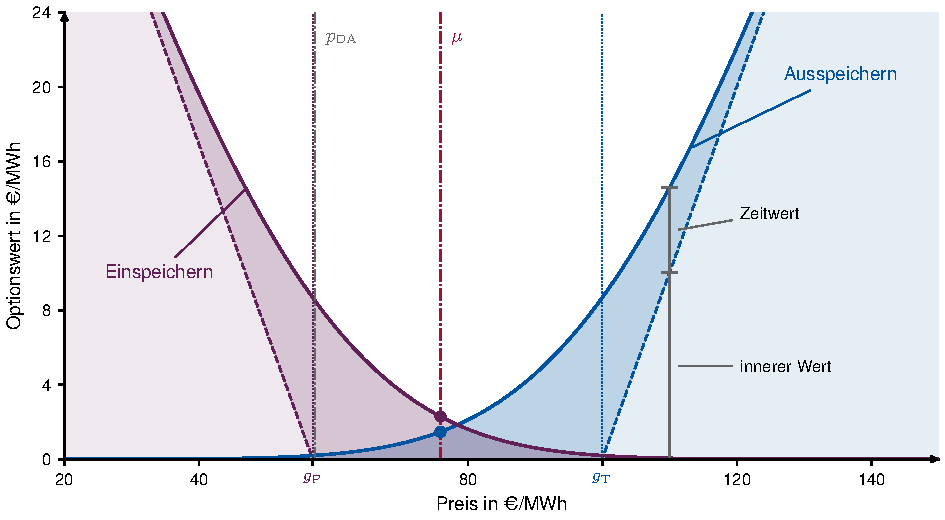
\includegraphics[width=\textwidth]{figures/chapter_2/weber_optionswert.pdf}
%    \caption{Wert der Aus- und der Einspeicheroption je \si{MW} und Viertelstunde über dem erwarteten Preisniveau für die Viertelstunde von 13:00 bis 13:15 Uhr des 01.02.2024, in der sich 0,369\,\si{\text{\euro}\per MW} und 0,573\,\si{\text{\euro}\per MW} ergeben. Nach \cite{bundesnetzagentur_berechnungsbeispiel_2024}.}
%    \label{fig:weber_optionswert}
%\end{figure}

%Ein veröffentlichtes Berechnungsbeispiel der \ac{BNetzA} führt das Verfahren für ein \ac{PSKW} vor \cite{bundesnetzagentur_berechnungsbeispiel_2024}.
%Betrachtet wird eine Anlage mit \SI{200}{\mega\watt} Turbinen- und \SI{180}{\mega\watt} Pumpleistung, deren Grenzpreise sich zu $g_T = 99{,}97\,\si{\text{\euro}\per MWh}$ und $g_P = 56{,}93\,\si{\text{\euro}\per MWh}$ ergeben.
%Für die Viertelstunde von 13:00 bis 13:15 Uhr betragen das erwartete Preisniveau $\mu = 75{,}93\,\si{\text{\euro}\per MWh}$ und das Volatilitätsmaß $\sigma = 21{,}75\,\si{\text{\euro}\per MWh}$.
%Beide sind auf dieses Viertelstundenprodukt bezogen, $\mu$ auf seine Eröffnungsauktion und $\sigma$ auf die Abweichung seines \ac{ID1} von dieser Auktion über die vorangegangenen 30 Tage.
%Der Day-Ahead-Preis liegt mit 57,26\,\si{\text{\euro}\per MWh} unter dem Grenzpreis der Turbine, sodass die Turbine bei wirtschaftlich optimalem Einsatz stillstünde, ihr nur die Aufnahme der Ausspeicherung offensteht und sie als Call bewertet wird.
%Zugleich liegt er über dem Grenzpreis der Pumpe, sodass auch die Pumpe stillstünde, ihr nur die Aufnahme der Einspeicherung offensteht und sie als Put bewertet wird, weil der Wert dieser Möglichkeit mit fallendem Preis steigt.
%Aus $\mu$ folgen mit Gleichung~\eqref{eq:weber_d} die standardisierten Abstände $d_T = -1{,}105$ und $d_P = 0{,}874$.
%Die Gleichungen~\eqref{eq:weber_call} und \eqref{eq:weber_put} liefern daraus $V_C = 1{,}477\,\si{\text{\euro}\per\text{(MW\,h)}}$ und $V_P = 2{,}292\,\si{\text{\euro}\per\text{(MW\,h)}}$, was nach Umrechnung auf die Produktdauer einer Viertelstunde 0,369\,\si{\text{\euro}\per MW} und 0,573\,\si{\text{\euro}\per MW} entspricht.
%Beide Optionen sind damit aus dem Geld, sodass der Betrag vollständig aus Zeitwert besteht.
%Abbildung~\ref{fig:weber_optionswert} gilt dabei allein für diese Viertelstunde, denn das Volatilitätsmaß wird je Viertelstundenprodukt bestimmt und jedes andere Produkt liegt daher auf einer anderen Kurve.
%Anhang~\ref{anh:weber} stellt das Verfahren einschließlich der Grenzpreisbestimmung und der Abrechnungspreise vollständig dar und wendet es auf eine zweite Viertelstunde sowie auf die Entscheidungslage des Betreibers entlang des Vortages an.

%Die je Viertelstunde und Richtung ermittelten Optionswerte werden mit der jeweils gesperrten Leistung multipliziert und dem anteiligen Werteverbrauch gegenübergestellt \cite{bundesnetzagentur_anlage1_2024}.
%Im Beispiel ergibt das bei vollständiger Sperrung beider Richtungen 73,83\,\si{\text{\euro}} und 103,13\,\si{\text{\euro}} und damit einen Gesamtbetrag von 176,96\,\si{\text{\euro}} für die eine Viertelstunde.
Die entgangenen Erlösmöglichkeiten sind der einzige Bestandteil des finanziellen Ausgleichs, der einen hypothetischen Marktverlauf bewerten muss.
Die Festlegung greift dafür auf eine finanzmathematische Bewertungslogik zurück, die einem Gutachten von Weber aus dem Jahr 2015 entstammt und der Festlegung als Anlage 2 beiliegt \cite{bundesnetzagentur_festlegung_2024, weber_gutachten_2015}.
Der Grundgedanke besteht darin, die Vermarktungsmöglichkeit einer flexiblen Anlage als Finanzoption aufzufassen.
Eine Option gewährt ein Recht ohne Pflicht.
Lohnt sich die Ausübung nicht, lässt der Inhaber die Option verfallen.
Eine Call-Option ist das Recht, zum Basispreis zu kaufen, und entspricht bei einer Anlage der Möglichkeit, bei steigendem Preis einzuspeisen.
Eine Put-Option ist das Recht, zum Basispreis zu verkaufen, und entspricht der Möglichkeit, vermarktete Leistung zurückzunehmen.

Das Gutachten bewertet die Vermarktungsmöglichkeit über einen Tag als Sequenz solcher Optionen und behandelt die einzelnen Intervalle als voneinander unabhängig.
Wird die Anlage durch eine Anweisung an der Ausübung gehindert, entspricht der entgangene Deckungsbeitrag dem Wert der verlorenen Option.
Ein Speicher trägt dabei zwei Optionen, denn er speist nicht nur ein, sondern bezieht auch.
Die Ausspeicher- und die Einspeicherseite tragen deshalb je eine eigene Option, deren Basispreis der obere beziehungsweise der untere Grenzpreis der Anlage ist.

Die Festlegung setzt diese Logik mit drei Eingangsgrößen um, nämlich dem dort als Strikepreis bezeichneten Basispreis, dem erwarteten Preisniveau und einem Volatilitätsmaß \cite{bundesnetzagentur_anlage1_2024}.
Der Basispreis ist bei Tagesspeichern einer der beiden Grenzpreise, die aus der nach dem Preis geordneten Reihe der Viertelstunden der \ac{IDA-1} folgen.
Dazu werden die teuersten Viertelstunden als Ausspeicherung mit den günstigsten als Einspeicherung zusammengeführt.
Das Verfahren endet, sobald die verfügbaren Volllaststunden, also der Energieinhalt je Leistung, ausgeschöpft sind oder der Erlös der Ausspeicherung die Kosten der Einspeicherung nicht mehr deckt.
Als erwartetes Preisniveau dient der Preis derselben Auktion.
Das Volatilitätsmaß ist die Standardabweichung der Differenz zwischen dem \ac{ID1} und dieser Auktion, rollierend über die jeweils letzten 30 Tage.
Anders als in der Optionsbewertung üblich wird das Volatilitätsmaß nicht auf die verbleibende Zeit bis zur Lieferung skaliert, denn es misst bereits die Abweichung über das feste Intervall vom Preis der \ac{IDA-1} bis zum \ac{ID1} \cite{hull_options_2014}.

% DURCHSICHT 16.09.2026, C1, Anknuepfung. Alte Fassung:
%Der Optionswert setzt sich aus dem inneren Wert und dem Zeitwert zusammen.
Aus den drei Eingangsgrößen ergibt sich der Optionswert, der sich aus dem inneren Wert und dem Zeitwert zusammensetzt.
Der innere Wert erfasst die bei sofortiger Ausübung anfallende Differenz zwischen erwartetem Preis und Basispreis, der Zeitwert die verbleibende Chance auf eine günstigere Preisentwicklung.
% DURCHSICHT 16.09.2026, C1, Begruendung angebunden. Alte Fassung:
%Der Zeitwert ist der Grund, weshalb die Festlegung überhaupt einen Optionsansatz verlangt.
Der Zeitwert ist der Grund, weshalb die Festlegung überhaupt einen Optionsansatz verlangt, denn eine Vergütung allein der Preisdifferenz zahlte für eine Viertelstunde mit einem erwarteten Preis zwischen den Grenzpreisen nichts.
% DURCHSICHT 16.09.2026, C1, im Vorsatz aufgegangen: Eine Vergütung allein der Preisdifferenz zahlte für eine Viertelstunde mit einem erwarteten Preis zwischen den Grenzpreisen nichts.
Dem Betreiber wird mit der Anweisung aber auch dort die Chance auf eine günstigere Preisentwicklung genommen.

Welche Optionsart eine Viertelstunde trägt, folgt aus dem Vergleich des stündlichen Day-Ahead-Preises mit dem Basispreis.
Die Festlegung unterstellt dabei einen gegenüber dem Day-Ahead-Preis optimalen Einsatz, sodass oberhalb des Basispreises nur die Rücknahme und unterhalb nur die Erhöhung der Einspeisung offensteht.
Die Begründung dieser Zuordnung mit den Differenzen zwischen Stunden- und Viertelstundenprodukten bezieht sich auf eine Marktstruktur, die seit der Umstellung des \ac{DA} auf Viertelstundenprodukte entfallen ist \cite{ffe_saegezahn_2026}.
Die Zuordnung selbst gilt fort, ihre Begründung trägt seit der Umstellung aber nicht mehr.
Die je Viertelstunde und Richtung ermittelten Optionswerte werden mit der jeweils gesperrten Leistung multipliziert und dem anteiligen Werteverbrauch gegenübergestellt.
% HIERHER VERSCHOBEN am 20.09.2026 aus 2.3.1, siehe Vermerk dort, Bezug auf die Optionswerte umgestellt.
% Alte Fassung:
%Die Festlegung bildet die entgangenen Erlösmöglichkeiten netto vom Strikepreis, sodass sie allein gegen den anteiligen Werteverbrauch antreten und nicht gegen die Summe aus Werteverbrauch und Erzeugungsauslagen, wie in Anhang~\ref{anh:weber} dargestellt.
Die Optionswerte sind dabei netto vom Strikepreis gebildet, sodass sie allein gegen den anteiligen Werteverbrauch antreten und nicht gegen die Summe aus Werteverbrauch und Erzeugungsauslagen.
% R-75 am 18.09.2026, Kontrolle durch Fable, Entscheidung des Verfassers: Anhaenge handeln nicht, Stilregel 10. Alte Fassung:
%Anhang~\ref{anh:weber} führt die Formelzeichen und Bewertungsgleichungen, die Herkunft des Zusatzes modifiziert und das veröffentlichte Berechnungsbeispiel der \ac{BNetzA} für ein \ac{PSKW} vollständig aus.
Die Formelzeichen und Bewertungsgleichungen, die Herkunft des Zusatzes modifiziert und das veröffentlichte Berechnungsbeispiel der \ac{BNetzA} für ein \ac{PSKW} stehen vollständig in Anhang~\ref{anh:weber}.

\subsection{Grenzen der Übertragbarkeit auf \acs{BESS}}
\label{sec:weber_limits}

% NEU GEFASST am 15.09.2026 nach dem Absatzplan im Sammelmodus.
% Befunde G36, P4, Stilregeln 5 und 17. Dreizehn Saetze in drei Absaetze, Umschlagpunkt als eigene Deutung, Satz zur verschobenen Einspeisung entfallen.
% Alte Fassung, nicht wieder aufnehmen:
%Die Übertragung auf ein \ac{BESS} stößt vor allem an einer Stelle an Grenzen, nämlich an der Kopplung der Viertelstunden über den Ladezustand. Das Verfahren bewertet jede Viertelstunde für sich und setzt damit voraus, dass die Intervalle voneinander unabhängig sind. Bei einem Speicher trifft das nur zu, solange der Energievorrat groß gegenüber der Leistung ist, und Weber begründet die Annahme eines über den Tag konstanten Grenzpreises ausdrücklich mit dieser Voraussetzung \cite{weber_gutachten_2015}. Bei einem \ac{BESS} mit wenigen Stunden Entladedauer ist sie nicht erfüllt, denn jede Ein- oder Ausspeisung verschiebt den Grenzpreis der folgenden Intervalle, und das Berechnungsbeispiel verortet den Umschlagpunkt zwischen vier und sechs Volllaststunden \cite{bundesnetzagentur_berechnungsbeispiel_2024}. Sichtbar wird die Kopplung zunächst an den Volllaststunden, denn sie begrenzen die Zahl der Iterationen und bestimmen darüber die beiden Grenzpreise, sodass wenige Volllaststunden diese auseinanderrücken und beide Optionen weiter aus dem Geld liegen. Sie zeigt sich zudem in einer Pfadabhängigkeit des Handlungsspielraums, denn ob eine Anlage in einem Intervall ausspeisen kann, hängt vom Ladezustand ab, den die vorangegangenen Entscheidungen hinterlassen haben. Weber benennt diese Vernachlässigung zeitübergreifender Restriktionen als Ursache einer tendenziellen Überschätzung der Optionalität \cite{weber_gutachten_2015}, und Untersuchungen zur Übertragbarkeit auf weitere Technologien bestätigen den Befund \cite{iaew_abschlussbericht_2023, iaew_folgestudie_2024}. Er nennt allerdings auch gegenläufige Vereinfachungen, nämlich die Vernachlässigung der ausgeprägten Ränder der Intraday-Preis\-verteilung und die Korrelation von Redispatcheingriffen mit windstarken Zeiten, sodass die Richtung der Gesamtabweichung nicht eindeutig ist. Ein Eingriff führt zudem meist nicht zu einer entfallenen, sondern zu einer verschobenen Ein- oder Ausspeisung, sodass der Nachteil in der schlechteren Preislage der Ersatzausübung liegt. Im Konsultationsverfahren ist die Kopplung über die Volllaststunden vorgetragen worden, nämlich dass der Weber-Ansatz schlecht passe, weil deren Zahl bei Batteriespeichern deutlich geringer sei als bei einem \ac{PSKW}. Die Beschlusskammer hat darauf mit der verwendeten Preisreihe geantwortet, nämlich dass auf den Preis der Viertelstundenprodukte im kontinuierlichen Intraday-Handel in der letzten Stunde vor Lieferung abgestellt werde und kurzfristige Erlösmöglichkeiten damit berücksichtigt seien \cite{bundesnetzagentur_anlage1_2024}. Diese Preisreihe bestimmt jedoch das erwartete Preisniveau, während die Volllaststunden über die Zahl der Iterationen die Grenzpreise festlegen, sodass die Erwiderung eine andere Eingangsgröße betrifft als der Einwand.

%Über die im Verfahren erhobenen Punkte hinaus tritt eine Überlegung zum Zeitwert. Der Wert der verbleibenden Optionalität nimmt zum Lieferzeitpunkt hin ab, weil weniger Handelsgelegenheiten offenstehen, das Volatilitätsmaß der Festlegung bleibt über den gesamten Vorlauf jedoch gleich. Eine Anweisung eine Viertelstunde vor der Lieferung wird deshalb mit demselben Zeitwert vergütet wie eine Stunde zuvor. Ein \ac{BESS} trifft das besonders, weil es seinen Betriebspunkt bis kurz vor die Lieferung offenhält und deshalb eher spät angewiesen wird.
Die Übertragung auf ein \ac{BESS} stößt vor allem an einer Stelle an Grenzen, nämlich an der Kopplung der Viertelstunden über den Ladezustand.
Das Verfahren bewertet jede Viertelstunde für sich und setzt damit voraus, dass die Intervalle voneinander unabhängig sind.
Bei einem Speicher gilt die Unabhängigkeit nur, solange der Energievorrat groß gegenüber der Leistung ist.
Weber begründet die Annahme eines über den Tag konstanten Grenzpreises ausdrücklich mit der Voraussetzung eines großen Energievorrats \cite{weber_gutachten_2015}.
Bei einem \ac{BESS} mit einem Energieinhalt je Leistung von ein bis zwei Stunden ist die Voraussetzung nicht erfüllt, denn jede Ein- oder Ausspeisung verschiebt den Grenzpreis der folgenden Intervalle.
% EIGENE DEUTUNG des Berechnungsbeispiels (P4), so benannt.
% I-20 am 17.09.2026, Kontrolle durch Fable, Entscheidung des Verfassers: kuerzen auf die vier Volllaststunden des Berechnungsbeispiels, denn die sechs sind nirgends hergeleitet. Alte Fassung:
%Nach eigener Deutung des Berechnungsbeispiels liegt der Umschlagpunkt zwischen vier und sechs Volllaststunden \cite{bundesnetzagentur_berechnungsbeispiel_2024}.
Das Berechnungsbeispiel rechnet mit vier Volllaststunden \cite{bundesnetzagentur_berechnungsbeispiel_2024}.
% S-21 am 18.09.2026, Kontrolle durch Fable, Entscheidung des Verfassers: gestrichen, die Aussage traegt der Satz zum Energieinhalt je Leistung im selben Absatz. Gestrichener Satz: Alte Fassung:
%\ac{BESS} am Netz liegen mit ein bis zwei Stunden darunter.

Sichtbar wird die Kopplung zunächst an den Volllaststunden, denn sie begrenzen die Zahl der Iterationen und bestimmen darüber die beiden Grenzpreise.
Wenige Volllaststunden rücken die Grenzpreise auseinander, sodass beide Optionen weiter aus dem Geld liegen, also keinen inneren Wert tragen.
Die Kopplung zeigt sich zudem in einer Pfadabhängigkeit des Handlungsspielraums.
Ob eine Anlage in einem Intervall ausspeisen kann, hängt vom Ladezustand nach den vorangegangenen Entscheidungen ab.
Weber benennt diese Vernachlässigung zeitübergreifender Restriktionen als Ursache einer tendenziellen Überschätzung der Optionalität.
Weber nennt allerdings auch gegenläufige Vereinfachungen, nämlich die Vernachlässigung der ausgeprägten Ränder der Intraday-Preis\-verteilung und die Korrelation von Redispatcheingriffen mit windstarken Zeiten.
Die Richtung der Gesamtabweichung ist deshalb nicht eindeutig, und Untersuchungen zur Übertragbarkeit auf weitere Technologien bestätigen den Befund \cite{iaew_abschlussbericht_2023, iaew_folgestudie_2024}.

% I-41 am 18.09.2026, Kontrolle durch Fable, Entscheidung des Verfassers: Akronym statt ausgeschriebenem Begriff, die Verstaerkung deutlich entfaellt, die stillgelegte Pruefmarke ist nicht mehr noetig. Alte Fassung:
%Im Konsultationsverfahren ist die Kopplung über die Volllaststunden vorgetragen worden: Der Weber-Ansatz passe schlecht, weil deren Zahl bei Batteriespeichern deutlich geringer sei als bei einem \ac{PSKW}. % pruefen: ok
Im Konsultationsverfahren ist die Kopplung über die Volllaststunden vorgetragen worden: Der Weber-Ansatz passe schlecht, weil deren Zahl bei \ac{BESS} geringer sei als bei einem \ac{PSKW}.
Die Beschlusskammer hat darauf mit der verwendeten Preisreihe geantwortet, nämlich dass auf den Preis der Viertelstundenprodukte im kontinuierlichen Intraday-Handel in der letzten Stunde vor Lieferung abgestellt werde \cite{bundesnetzagentur_anlage1_2024}.
Die genannte Preisreihe bestimmt jedoch das erwartete Preisniveau, während die Volllaststunden über die Zahl der Iterationen die Grenzpreise festlegen.
Die Erwiderung betrifft damit eine andere Eingangsgröße als der Einwand, und der Einwand ist unbeantwortet geblieben.
Über die im Verfahren erhobenen Punkte hinaus tritt eine Überlegung zum Zeitwert.
Der Wert der verbleibenden Optionalität nimmt zum Lieferzeitpunkt hin ab, weil weniger Handelsgelegenheiten offenstehen.
Das Volatilitätsmaß der Festlegung bleibt über den gesamten Vorlauf jedoch gleich, sodass eine Anweisung eine Viertelstunde vor der Lieferung mit demselben Zeitwert vergütet wird wie eine Stunde zuvor.
% S-09 am 18.09.2026, Kontrolle durch Fable, Entscheidung des Verfassers: gestrichen, die Aussage traegt 2.3.3. Gestrichener Satz: Alte Fassung:
%Der gleichbleibende Zeitwert trifft ein \ac{BESS} besonders, weil es seinen Betriebspunkt bis kurz vor die Lieferung offenhält und deshalb eher spät angewiesen wird.

% NEU GEFASST am 15.09.2026 nach dem Absatzplan im Sammelmodus.
% Befund G37, Stilregeln 5 und 17. Anreizwirkung gekuerzt, lange Saetze geteilt.
% Alte Fassung, nicht wieder aufnehmen:
%Daraus folgt zugleich eine Anreizwirkung, denn eine kurzfristig angewiesene Anpassung wird ebenso vergütet wie eine früh angekündigte.
%Der Betreiber setzt seinen Fahrplan im Selbstdispatch selbst, und der Ausgleich stellt ihn anschließend so, als hätte er ihn behalten.
%Er kann deshalb hinter einem Engpass gezielt so einspeisen, dass ein Eingriff wahrscheinlich wird, und an der Differenz zwischen Marktpreis und Ausgleich verdienen.
%Dieses als inc-dec bezeichnete Verhalten setzt an der selbst gewählten Menge an und nicht an der Bewertungsformel, gewinnt aber an Gewicht, soweit diese die Optionalität überschätzt.
%Ein thermisches Kraftwerk ist in seiner Fahrweise durch Mindestlast, Anfahrkosten und Rampen gebunden, während ein Speicher seinen Fahrplan innerhalb seines Energieinhalts frei setzt und einen Betriebspunkt hinter dem Engpass ohne zusätzlichen Aufwand einnehmen kann.
%Die kostenbasierte Bemessung soll ein solches Verhalten gerade verhindern, für diese Technologie setzt sie jedoch selbst einen Anreiz dazu.

%Konsequenterweise hat die Beschlusskammer die Behandlung von \ac{BESS} in der Festlegung nicht abschließend geregelt, sondern ausdrücklich einer späteren Mitteilung vorbehalten \cite{bundesnetzagentur_festlegung_2024}.
%Damit ist die Bemessung bei \ac{BESS} bereits für den angeordneten Redispatch nicht eindeutig geklärt, sodass sie keinen Anhalt dafür bietet, wie eine kurative Vorhaltung dieser Anlagen zu vergüten wäre.
%Die Einwände betreffen dabei nicht die Wahl der Verteilungsannahme oder die Parametrisierung, sondern die Zerlegung in unabhängige Intervalle.
%Eine Option bewertet die Unsicherheit eines einzelnen Lieferintervalls, während der Wert eines Speichers daraus entsteht, dass er Arbeit zwischen Intervallen und zwischen Märkten verschiebt.
%Eine Anpassung der Formel griffe deshalb zu kurz.
%Hirth und andere beschreiben für den marktbasierten Redispatch strukturelle Anreize für ein engpassverstärkendes Bietverhalten \cite{hirth_kosten_2019}.
%Ein marktbasierter Redispatch ist mit einer marktbasierten kurativen Vorhaltung jedoch nicht gleichzusetzen, denn diese reserviert allein Leistung, während der Redispatch stets zugleich eine Energielieferung auslöst.
%Zu bestimmen ist zunächst, wie ein \ac{BESS} seine Flexibilität über den Tag tatsächlich einsetzt und welchen Beitrag die einzelnen Vermarktungswege dabei tragen, denn erst daraus folgt, was eine Bindung dieser Flexibilität kostet.
Daraus folgt zugleich eine Anreizwirkung, denn eine kurzfristig angewiesene Anpassung wird ebenso vergütet wie eine früh angekündigte.
Der Ausgleich stellt den Betreiber anschließend so, als hätte er seinen selbst gesetzten Fahrplan behalten.
Der Betreiber kann deshalb hinter einem Engpass gezielt so einspeisen, dass ein Eingriff wahrscheinlich wird, und an der Differenz zwischen Marktpreis und Ausgleich verdienen.
% I-42 am 18.09.2026, Kontrolle durch Fable, Entscheidung des Verfassers: eine Schreibweise, Inc-Dec, hier und in Anhang A. Alte Fassung:
%Das inc-dec genannte Verhalten, also die gezielte Erhöhung der Einspeisung vor einem erwarteten Eingriff, setzt an der selbst gewählten Menge an und nicht an der Bewertungsformel.
Das Inc-Dec genannte Verhalten, also die gezielte Erhöhung der Einspeisung vor einem erwarteten Eingriff, setzt an der selbst gewählten Menge an und nicht an der Bewertungsformel.
Das Verhalten gewinnt aber an Gewicht, soweit die Formel die Optionalität überschätzt.
Ein thermisches Kraftwerk ist in seiner Fahrweise durch Mindestlast, Anfahrkosten und Rampen gebunden.
Ein Speicher setzt seinen Fahrplan dagegen innerhalb seines Energieinhalts frei und kann einen Betriebspunkt hinter dem Engpass ohne zusätzlichen Aufwand einnehmen.
Die kostenbasierte Bemessung soll ein solches Verhalten gerade verhindern, für Speicher setzt sie jedoch selbst einen Anreiz dazu.

% DURCHSICHT 16.09.2026, C1. Alte Fassung:
%Konsequenterweise hat die Beschlusskammer die Behandlung von \ac{BESS} in der Festlegung nicht abschließend geregelt, sondern ausdrücklich einer späteren Mitteilung vorbehalten \cite{bundesnetzagentur_festlegung_2024}.
Die Beschlusskammer hat die Behandlung von \ac{BESS} in der Festlegung nicht abschließend geregelt, sondern ausdrücklich einer späteren Mitteilung vorbehalten \cite{bundesnetzagentur_festlegung_2024}.
Damit ist die Bemessung bei \ac{BESS} bereits für den angeordneten Redispatch nicht eindeutig geklärt.
Die Bemessung bietet deshalb keinen Anhalt dafür, wie eine kurative Vorhaltung dieser Anlagen zu vergüten wäre.
% DURCHSICHT 16.09.2026, C1, Stilregel 5. Alte Fassung:
%Die Einwände betreffen dabei nicht die Wahl der Verteilungsannahme oder die Parametrisierung, sondern die Zerlegung in unabhängige Intervalle.
Die genannten Einwände betreffen nicht die Wahl der Verteilungsannahme oder die Parametrisierung, sondern die Zerlegung in unabhängige Intervalle.
Eine Option bewertet die Unsicherheit eines einzelnen Lieferintervalls, während der Wert eines Speichers daraus entsteht, dass er Arbeit zwischen Intervallen und zwischen Märkten verschiebt.
Eine Anpassung der Formel griffe deshalb zu kurz.

% NEUER ABSATZ 16.09.2026, C2.9.
% DURCHSICHT 16.09.2026, C1, Anknuepfung. Alte Fassung:
%Hirth und andere beschreiben für den marktbasierten Redispatch strukturelle Anreize für ein engpassverstärkendes Bietverhalten \cite{hirth_kosten_2019}.
Ein weiterer Einwand stammt aus der Debatte um den marktbasierten Redispatch: Hirth und andere beschreiben dort strukturelle Anreize für ein engpassverstärkendes Bietverhalten \cite{hirth_kosten_2019}.
% R-44 am 18.09.2026, Kontrolle durch Fable, Entscheidung des Verfassers: die Begruendung steht auf dem belastbaren Kern. Alte Fassung:
%Der Einwand trifft die Vergütung eines Eingriffs, und eine marktbasierte kurative Vorhaltung reserviert dagegen allein Leistung.
Der Einwand trifft die Vergütung eines Eingriffs, während die Vergütung der kurativen Vorhaltung unabhängig vom Abruf anfällt.
% R-44 am 18.09.2026, Kontrolle durch Fable, Entscheidung des Verfassers: die Begruendung ueber die Energielieferung traegt nicht, denn auch der kurative Abruf liefert Energie. Alte Fassung:
%Der Redispatch löst stets zugleich eine Energielieferung aus, weshalb der Einwand nicht ohne Weiteres übertragbar ist.
Ob von der Vergütung eines Abrufs ein eigener Anreiz ausgeht, ist gesondert zu prüfen.
% DURCHSICHT 16.09.2026, C1. Alte Fassung:
%Zu bestimmen ist zunächst, wie ein \ac{BESS} seine Flexibilität über den Tag einsetzt und welchen Beitrag die einzelnen Vermarktungswege tragen.
Für die kurative Vorhaltung ist deshalb zunächst zu bestimmen, wie ein \ac{BESS} seine Flexibilität über den Tag einsetzt und welchen Beitrag die einzelnen Vermarktungswege tragen.
Erst daraus folgt, was eine Bindung dieser Flexibilität kostet.

% UMBENANNT am 15.09.2026 auf Vorgabe des Verfassers, weil der Abschnitt die mFRR abgrenzt. Alte Fassung:
%\subsection{Vergütung von \acs{FCR} und \acs{aFRR}}
\subsection{Vergütung der Regelleistung}
\label{sec:balancing_procurement}
% NEU GEFASST am 15.09.2026 nach dem Absatzplan im Sammelmodus.
% Kuerzung A3, Stilregeln 5 und 17. Zuschlagspflicht und Praequalifikation stehen in 2.2.3, Verweis auf die entfallene Tabelle gestrichen, lange Saetze geteilt.
% Alte Fassung, nicht wieder aufnehmen:
%Regelleistung wird beschafft, bevor feststeht, ob und in welchem Umfang sie gebraucht wird.
%Der Zuschlag verpflichtet den Anbieter deshalb, die zugesagte Leistung über die gesamte Erbringungsperiode bereitzuhalten und einen Abruf nicht abzulehnen.
%Vergütet wird dafür der Leistungspreis, und bei der \ac{aFRR} tritt für die tatsächlich abgerufene Arbeit ein Arbeitspreis hinzu, während die \ac{FCR} ohne gesonderte Arbeitsvergütung auskommt.
%Der Arbeitspreis der \ac{aFRR} entsteht nicht in einer Auktion des Vortages, sondern über die europäische Plattform PICASSO, auf der seit dem Jahr 2022 \ac{aFRR}-Regelarbeit ausgetauscht wird \cite{bundesnetzagentur_monitoringbericht_2026}.
%Am Regelarbeitsmarkt kann jede präqualifizierte Einheit für jedes Viertelstundenfenster ein Energiegebot abgeben.
%Wer einen Zuschlag für \ac{aFRR}-Leistung erhalten hat, ist für die reservierte Leistung zur Abgabe eines Arbeitspreisgebotes verpflichtet, während die übrigen Anbieter Menge und Preis frei wählen.
%Damit ist die benötigte Energie gesichert, ohne den Zugang zum Abruf zu verengen, und der Zuschlag erfolgt 25 Minuten vor Beginn der Produktzeitscheibe.
%Hält der Anbieter die zugesagte Leistung nicht vor, rechnet der \ac{ÜNB} eine Anreizkomponente ab, und zwar bereits dann, wenn die Leistung für einen Abruf nicht zur Verfügung gestanden hätte.
%Der Leistungspreis vergütet damit die Übernahme des Verfügbarkeitsrisikos und nicht den Abruf, der überwiegend ausbleibt.

%Für einen Speicher hat das eine Folge, die andere Technologien nicht kennen.
%Er kann die zugesagte Leistung nur erbringen, wenn im Abrufzeitpunkt der erforderliche Energieinhalt vorhanden ist, weshalb er seinen Ladezustand über die gesamte Erbringungsperiode in einem Bereich halten muss, dessen Untergrenze das Präqualifikationsverfahren nach Abschnitt~\ref{sec:ancillary_services} vorgibt.
%Bei der \ac{FCR} muss er die zugesagte Leistung mindestens 15 Minuten durchgehend vollständig erbringen können \cite{bundesnetzagentur_beschluss_2019}, bei der \ac{aFRR} 60 Minuten bezogen auf die vermarktete Leistung.
%Ein Speicher mit einer Stunde Entladedauer bindet damit bei der \ac{aFRR} seinen gesamten Energieinhalt für die zugesagte Leistung. Tabelle~\ref{tab:balancing_remuneration} fasst die Vergütungsbestandteile zusammen.

%Für die vorliegende Arbeit ist daran dreierlei bedeutsam.
%Erstens belegt die \ac{FCR}, dass die Vergütung vorgehaltener und überwiegend nicht abgerufener Leistung regulatorisch etabliert und wettbewerblich organisierbar ist.
%Zweitens zeigt die \ac{aFRR}, dass sich Vorhaltung und Abruf getrennt bepreisen lassen, was der Struktur einer kurativen Zusage entspricht, die über die gesamte Bindungsdauer besteht, während ein Abruf nur im Fehlerfall erfolgt, und dass sich die Gebotspflicht dabei auf die bezuschlagte Leistung beschränken lässt, ohne den Zugang zum Abruf zu verengen.
%Drittens ist die Bindung eines Ladezustandsbereichs über eine feste Erbringungsperiode bereits Bestandteil eines bestehenden Produkts und keine Besonderheit des kurativen Marktmechanismus.
%Die Beschaffungslogik der Regelleistung ist damit auf die kurative Vorhaltung nicht unmittelbar anwendbar, liefert aber die Form, an der sich der kurative Marktmechanismus orientieren kann.
% ERGAENZT am 15.09.2026 auf Vorgabe des Verfassers, Abgrenzung der mFRR aus 2.2.3 hierher verschoben. Zahlen aus analysen/mfrr_leistungspreise, eigene Auswertung der Ausschreibungsergebnisse 2025.
Für ein \ac{BESS} sind von den drei Produkten die \ac{FCR} und die \ac{aFRR} von Belang, denn die \ac{mFRR} bietet bei gleichem Produktschnitt den geringeren Leistungspreis.
% EINHEIT ALS SYMBOL am 17.09.2026, Kommentar des Verfassers. Alte Fassung:
%Im Jahr 2025 lag der mittlere Leistungspreis der \ac{mFRR} nach eigener Auswertung der Ausschreibungsergebnisse bei 5 Euro je Megawatt und Stunde in positiver und 11 Euro je Megawatt und Stunde in negativer Richtung, der der \ac{aFRR} bei 18 Euro je Megawatt und Stunde und 16 Euro je Megawatt und Stunde \cite{regelleistung_ausschreibungsdaten_2026}.
Im Jahr 2025 lag der mittlere Leistungspreis der \ac{mFRR} nach eigener Auswertung der Ausschreibungsergebnisse bei 5\,\EurMWh{} in positiver und 11\,\EurMWh{} in negativer Richtung, der der \ac{aFRR} bei 18\,\EurMWh{} und 16\,\EurMWh{} \cite{regelleistung_ausschreibungsdaten_2026}.
% GESTRICHEN am 15.09.2026 auf Vorgabe des Verfassers, der Erloesindex ist erst in 3.3.1 eingefuehrt. Nicht wieder aufnehmen:
%Der Erlösindex, der die Erlöse von \ac{BESS} am deutschen Markt ausweist, führt die \ac{mFRR} ebenfalls nicht \cite{isea_methodik_2026}.
Die \ac{mFRR} bleibt deshalb im Weiteren außer Betracht.
% ABSATZ VERBUNDEN 16.09.2026, C2.11.
Anders als das Engpassmanagement vergütet die Regelleistung die Vorhaltung selbst, und zwar über den Leistungspreis für die zugesagte Leistung.
Bei der \ac{aFRR} tritt für die tatsächlich abgerufene Arbeit ein Arbeitspreis hinzu, während die \ac{FCR} ohne gesonderte Arbeitsvergütung auskommt.
% UMBAU am 20.09.2026, Vorgabe des Verfassers: "ich wollte im Kapitel 2.2.1 die Zeitschienen haben ... fuege die Zeitschienen fuer Regelleistung und Redispatch in 2.2.1 ein und versuche, so wenig wie moeglich darauf in 2.2.2 einzugehen. 2.2.2 soll eher erklaeren, was dort gemacht wird, wie der Rahmen ist, wofuer und wer daran teilnimmt, aber so wenig wie moeglich Verguetung."
% Rahmenaussage, Plattform PICASSO steht in 2.2.2 beim Abruf. Nicht wieder aufnehmen:
%Der Arbeitspreis der \ac{aFRR} entsteht nicht in einer Auktion des Vortages, sondern über die europäische Plattform PICASSO, auf der seit dem Jahr 2022 \ac{aFRR}-Regelarbeit ausgetauscht wird \cite{bundesnetzagentur_monitoringbericht_2026}.
% UMBAU am 20.09.2026, Vorgabe des Verfassers: "ich wollte im Kapitel 2.2.1 die Zeitschienen haben ... fuege die Zeitschienen fuer Regelleistung und Redispatch in 2.2.1 ein und versuche, so wenig wie moeglich darauf in 2.2.2 einzugehen. 2.2.2 soll eher erklaeren, was dort gemacht wird, wie der Rahmen ist, wofuer und wer daran teilnimmt, aber so wenig wie moeglich Verguetung."
% Rahmenaussage, jetzt in 2.2.2. Nicht wieder aufnehmen:
%Am Regelarbeitsmarkt kann jede präqualifizierte Einheit für jedes Viertelstundenfenster ein Energiegebot abgeben.
% UMBAU am 20.09.2026, Vorgabe des Verfassers: "ich wollte im Kapitel 2.2.1 die Zeitschienen haben ... fuege die Zeitschienen fuer Regelleistung und Redispatch in 2.2.1 ein und versuche, so wenig wie moeglich darauf in 2.2.2 einzugehen. 2.2.2 soll eher erklaeren, was dort gemacht wird, wie der Rahmen ist, wofuer und wer daran teilnimmt, aber so wenig wie moeglich Verguetung."
% Rahmenaussage, jetzt in 2.2.2. Nicht wieder aufnehmen:
%Wer einen Zuschlag für \ac{aFRR}-Leistung erhalten hat, ist für die reservierte Leistung zur Abgabe eines Arbeitspreisgebotes verpflichtet.
% SACHFEHLER BEHOBEN am 19.09.2026, Befund der Zahlenpruefung: die 25 Minuten sind nicht der
% Zuschlag, sondern der Gebotsabgabeschluss des Regelarbeitsmarkts. Monitoringbericht 2025, S. 123:
% "Der RAM oeffnet nach Verkuendung der RLM-Auktionsergebnisse und schliesst 25 Minuten vor Beginn
% der jeweiligen Produktzeitscheibe." Ein Zuschlag findet zu diesem Zeitpunkt nicht statt, die
% Aktivierung laeuft waehrend der Zeitscheibe fortlaufend ueber PICASSO, und die Verguetung folgt
% dem Grenzpreisverfahren, wie der uebernaechste Satz sagt. ACHTUNG: dieselbe Verwechslung steht
% noch in den auskommentierten Zeilen mit der Tabellenfussnote und der Beschaffungszeile, sie darf
% von dort nicht wieder aufgenommen werden. Alte Fassung, nicht wieder aufnehmen:
%Die übrigen Anbieter wählen Menge und Preis frei, und der Zuschlag erfolgt 25 Minuten vor Beginn der Produktzeitscheibe.
% UMBAU am 20.09.2026, Vorgabe des Verfassers: "ich wollte im Kapitel 2.2.1 die Zeitschienen haben ... fuege die Zeitschienen fuer Regelleistung und Redispatch in 2.2.1 ein und versuche, so wenig wie moeglich darauf in 2.2.2 einzugehen. 2.2.2 soll eher erklaeren, was dort gemacht wird, wie der Rahmen ist, wofuer und wer daran teilnimmt, aber so wenig wie moeglich Verguetung."
% Rahmenaussage, Handelsschluss jetzt in 2.2.1. Nicht wieder aufnehmen:
%Die übrigen Anbieter wählen Menge und Preis frei, und der Regelarbeitsmarkt schließt 25 Minuten vor Beginn der Produktzeitscheibe.
% ERGAENZT am 17.09.2026, Kommentar des Verfassers: die Verguetungsregel der Regelarbeit gehoert nach Kapitel 2. Beleg: Verordnung (EU) 2017/2195, Seite 28, Grenzpreisverfahren.
Abgerufene Arbeitsgebote vergütet der \ac{ÜNB} nach dem Grenzpreisverfahren, also alle zum Preis des teuersten abgerufenen Gebots \cite{europaische_kommission_verordnung_2017_ebgl}.
Das Arbeitspreisgebot entscheidet damit über den Abruf und nicht über die Höhe der Vergütung.
Damit ist die benötigte Energie gesichert, ohne den Zugang zum Abruf zu verengen.

% DURCHSICHT 16.09.2026, C1, Anknuepfung. Alte Fassung:
%Hält der Anbieter die zugesagte Leistung nicht vor, rechnet der \ac{ÜNB} eine Anreizkomponente ab.
% I-40 am 18.09.2026, Kontrolle durch Fable, Entscheidung des Verfassers: die Anreizkomponente stand ohne Quelle, sie steht in den Praequalifikationsbedingungen. Alte Fassung:
%Der Leistungspreis ist an die Vorhaltung gebunden: Hält der Anbieter die zugesagte Leistung nicht vor, rechnet der \ac{ÜNB} eine Anreizkomponente ab.
Der Leistungspreis ist an die Vorhaltung gebunden: Hält der Anbieter die zugesagte Leistung nicht vor, rechnet der \ac{ÜNB} eine Anreizkomponente ab \cite{ubertragungsnetzbetreiber_deutschland_praqualifikationsverfahren_2024}.
Die Anreizkomponente fällt bereits an, wenn die Leistung für einen Abruf nicht zur Verfügung gestanden hätte.
Der Leistungspreis vergütet damit die Übernahme des Verfügbarkeitsrisikos und nicht den Abruf, der überwiegend ausbleibt.
Für einen Speicher hat die Vorhaltepflicht eine Folge, die andere Technologien nicht kennen.
Der Speicher kann die zugesagte Leistung nur erbringen, wenn im Abrufzeitpunkt der erforderliche Energieinhalt vorhanden ist.
Der Speicher muss seinen Ladezustand deshalb über die gesamte Erbringungsperiode in einem Bereich halten, dessen Untergrenze das Präqualifikationsverfahren vorgibt.
% BEZUGSGROESSE UND BELEG BERICHTIGT am 19.09.2026, Befund der Zahlenpruefung. Erstens beziehen
% sich die 15 Minuten auf die praequalifizierte Leistung und nicht auf die zugesagte.
% PQ-Bedingungen 2024, Abschn. 2.7.1, S. 40: "Das minimale Arbeitsvermoegen des Energiespeichers
% relativ zur PQ-Leistung betraegt im Falle der FCR und im Falle der FRR jeweils 15 Minuten." Und
% fuer die FRR: "Im Falle der FRR betraegt das minimale Arbeitsvermoegen des Energiespeichers
% relativ zur Vermarktbaren Leistung 60 Minuten." Zweitens trug bundesnetzagentur_beschluss_2019
% die 15 Minuten nur mittelbar, denn der Beschluss BK6-17-234 lehnt allein einen Antrag auf
% 30 Minuten ab und verweist im Uebrigen auf die Auffangregel der SO GL. Die PQ-Bedingungen selbst
% nennen als Rechtsgrundlage die "Mindestaktivierungszeit von 15 Minuten gemaess Artikel 156
% Absatz 9", deshalb steht hier jetzt die SO GL. Die PQ-Bedingungen sind im selben Absatz bereits
% belegt, Stilregel 15. HINWEIS: bundesnetzagentur_beschluss_2019 wird damit nirgends mehr
% zitiert, der Eintrag in literature.bib bleibt vorerst stehen. Alte Fassung:
%Bei der \ac{FCR} muss der Speicher die zugesagte Leistung mindestens 15 Minuten durchgehend vollständig erbringen können \cite{bundesnetzagentur_beschluss_2019}, bei der \ac{aFRR} 60 Minuten bezogen auf die vermarktete Leistung.
Bei der \ac{FCR} muss der Speicher ein Arbeitsvermögen von mindestens 15 Minuten bezogen auf die präqualifizierte Leistung vorhalten \cite{europaische_kommission_verordnung_2017}, bei der \ac{aFRR} von 60 Minuten bezogen auf die vermarktete Leistung.
Ein Speicher mit einem Energieinhalt je Leistung von einer Stunde bindet damit bei der \ac{aFRR} seinen gesamten Energieinhalt für die zugesagte Leistung.

Für den kurativen Marktmechanismus ist daran dreierlei bedeutsam.
Erstens belegt die \ac{FCR}, dass die Vergütung vorgehaltener und überwiegend nicht abgerufener Leistung regulatorisch etabliert und wettbewerblich organisierbar ist.
Zweitens zeigt die \ac{aFRR}, dass sich Vorhaltung und Abruf getrennt bepreisen lassen.
Eine kurative Zusage hat dieselbe Struktur, denn sie besteht über die gesamte Bindungsdauer und ein Abruf erfolgt nur im Fehlerfall.
Die \ac{aFRR} zeigt zudem, dass sich die Gebotspflicht auf die bezuschlagte Leistung beschränken lässt, ohne den Zugang zum Abruf zu verengen.
Drittens ist die Bindung eines Ladezustandsbereichs über eine feste Erbringungsperiode bereits Bestandteil eines bestehenden Produkts und keine Besonderheit des kurativen Marktmechanismus.
% DURCHSICHT 16.09.2026, C1, Grund im Absatz. Alte Fassung:
%Die Beschaffungslogik der Regelleistung ist damit auf die kurative Vorhaltung nicht unmittelbar anwendbar, liefert aber die Form, an der sich der kurative Marktmechanismus orientieren kann.
Die Beschaffungslogik der Regelleistung ist auf die kurative Vorhaltung nicht unmittelbar anwendbar, weil sie keinen Bezug zum Netzknoten kennt, liefert aber die Form, an der sich der kurative Marktmechanismus orientieren kann.

% TABELLE ENTFALLEN am 15.09.2026, Kuerzung A3. Die Bemessung steht als Spalte in tab:regelleistung. Alte Fassung:
%\begin{table}[htbp]
%    \centering
%    \caption{Vergütungsbestandteile der \ac{FCR} und der \ac{aFRR} im Vergleich.}
%    \label{tab:balancing_remuneration}
%    \small
%    \begin{tabular}{@{}>{\raggedright\arraybackslash}p{\dimexpr0.22\textwidth-\tabcolsep\relax}>{\raggedright\arraybackslash}p{\dimexpr0.26\textwidth-2\tabcolsep\relax}>{\raggedright\arraybackslash}p{\dimexpr0.26\textwidth-2\tabcolsep\relax}>{\raggedright\arraybackslash}p{\dimexpr0.26\textwidth-\tabcolsep\relax}@{}}
%        \hline
%        \textbf{Merkmal} & \textbf{\acs{FCR}} & \textbf{\acs{aFRR} Leistung} & \textbf{\acs{aFRR} Arbeit} \\
%        \hline
%        Beschaffung & 8 Uhr des Vortages & 9 Uhr des Vortages & 25 Minuten vor Beginn \\
%        \hline
%        Bemessungsgröße & zugesagte Leistung & zugesagte Leistung & abgerufene Arbeit \\
%        \hline
%        Zeitbezug & je Zeitscheibe & je Zeitscheibe & je Viertelstunde \\
%        \hline
%        Eintritt & sicher & sicher & nur bei Abruf \\
%        \hline
%    \end{tabular}
%\end{table}

\subsection{Wettbewerb um Leistung und Ladezustand}
\label{sec:revenue_stacking}
\label{sec:soc_conflict}
\label{sec:market_development}

% GEKUERZT am 15.09.2026, Q18, die 564 MW stehen in 2.2.3. Alte Fassung:
%Ein \ac{BESS} erwirtschaftet seine Erlöse nicht aus einer einzelnen Anwendung, sondern aus mehreren parallelen Vermarktungswegen. Die beiden Hauptquellen sind die Arbitrage auf den Spotmärkten und die Vorhaltung von Regelleistung, deren Vergütung Abschnitt~\ref{sec:balancing_procurement} darstellt. Die gleichzeitige Nutzung mehrerer Wege, im Folgenden als Mehrfachvermarktung bezeichnet und in der Literatur als Multi-Use geführt, gilt als Voraussetzung eines wirtschaftlich robusten Betriebs \cite{celi_cortes_m5use_2024}. Wie stark der Wettbewerb um diese Erlösquellen inzwischen ist, zeigt die \ac{FCR}, für die im Jahr 2024 bereits 810\,\si{MW} an \ac{BESS} präqualifiziert waren, während der gesamte deutsche Bedarf bei 564\,\si{MW} lag \cite{celi_cortes_m5use_2024}.
% DURCHSICHT 16.09.2026, Befund des Verfassers: Arbitrage bei der ersten Verwendung erklaert. Alte Fassung:
%Ein \ac{BESS} erwirtschaftet seine Erlöse nicht aus einer einzelnen Anwendung, sondern aus mehreren parallelen Vermarktungswegen. Die beiden Hauptquellen sind die Arbitrage auf den Spotmärkten und die Vorhaltung von Regelleistung, deren Vergütung Abschnitt~\ref{sec:balancing_procurement} darstellt. Die gleichzeitige Nutzung mehrerer Wege, im Folgenden als Mehrfachvermarktung bezeichnet und in der Literatur als Multi-Use geführt, gilt als Voraussetzung eines wirtschaftlich robusten Betriebs \cite{celi_cortes_m5use_2024}. Wie stark der Wettbewerb um diese Erlösquellen inzwischen ist, zeigt die \ac{FCR}, für die im Jahr 2024 bereits 810\,\si{MW} an \ac{BESS} präqualifiziert waren und damit mehr als der gesamte deutsche Bedarf \cite{celi_cortes_m5use_2024}.
Ein \ac{BESS} erwirtschaftet seine Erlöse nicht aus einer einzelnen Anwendung, sondern aus mehreren parallelen Vermarktungswegen. Die beiden Hauptquellen sind die Arbitrage auf den Spotmärkten, also das Einspeichern in Niedrigpreisphasen und das Ausspeichern in Hochpreisphasen, und die Vorhaltung von Regelleistung, deren Vergütung Abschnitt~\ref{sec:balancing_procurement} darstellt. Die gleichzeitige Nutzung mehrerer Wege, im Folgenden als Mehrfachvermarktung bezeichnet und in der Literatur als Multi-Use geführt, gilt als Voraussetzung eines wirtschaftlich robusten Betriebs \cite{celi_cortes_m5use_2024}. Wie stark der Wettbewerb um diese Erlösquellen inzwischen ist, zeigt die \ac{FCR}, für die im Jahr 2024 bereits 810\,\si{MW} an \ac{BESS} präqualifiziert waren und damit mehr als der gesamte deutsche Bedarf \cite{celi_cortes_m5use_2024}.
% ABSATZ VERBUNDEN 16.09.2026, C2.12.
Die parallelen Vermarktungswege greifen dabei nicht auf getrennte Ressourcen zu, sondern auf dieselbe Leistung und denselben Energieinhalt derselben Anlage. Der Umfang der parallel vermarktbaren Leistung ist deshalb begrenzt, und die Präqualifikationsbedingungen der Regelleistung bemessen die dort anrechenbare Leistung nach dem Arbeitsvermögen und den vorgesehenen Speichermanagementmaßnahmen \cite{ubertragungsnetzbetreiber_deutschland_praqualifikationsverfahren_2024}. Die am Regelleistungsmarkt bereitgestellte Leistungsscheibe wird dabei nicht für Redispatch-Maßnahmen herangezogen \cite{bundesnetzagentur_anlage1_2024}. Wie eng die Wege zusammenhängen, zeigt eine Optimierungsrechnung für einen Speicher am deutschen Markt, in der der Handel im \ac{IDC} teilweise dazu dient, den Ladezustand in dem für die Regelleistung erforderlichen Bereich zu halten \cite{celi_cortes_m5use_2024}. Leistung und Speicherkapazität sind damit die knappen Ressourcen, um die alle Vermarktungswege konkurrieren, und eine kurative Vorhaltung erhebt darauf einen weiteren Anspruch.

% SATZLAENGE am 15.09.2026, Stilregel 17, alte Fassung als Kommentar:
%Innerhalb des Ladezustandsbereichs, der nicht durch eine Vorhaltung gebunden ist, führt der marktoptimale Fahrplan den Ladezustand systematisch an dessen Ränder, weil Arbitrage gerade darin besteht, den Speicher in Niedrigpreisphasen zu füllen und in Hochpreisphasen zu leeren. Ein netzdienlicher Beitrag lässt sich folglich nur über eine Anpassung der Einsatzplanung und nicht als nachgelagerter Eingriff erreichen \cite{lindner_operation_2023, sous_untersuchung_2022}. Wie sich Leistung und Energieinhalt auf die einzelnen Märkte verteilen, ist dabei keine feste Größe. Der Betreiber entscheidet im Selbst\-dispatch-Modell allein erlösorientiert und verschiebt die Anteile, sobald sich die relativen Preise zwischen Arbitrage und Regelleistung ändern. Weil die Handelsgelegenheiten zeitlich versetzt liegen, trifft er jede dieser Entscheidungen zudem unter Unsicherheit über die folgenden. Was eine kurative Bindung den Betreiber kostet, hängt damit davon ab, welche Vermarktung er andernfalls gewählt hätte, und diese Alternative wechselt mit den relativen Preisen.
Innerhalb des Ladezustandsbereichs, der nicht durch eine Vorhaltung gebunden ist, führt der marktoptimale Fahrplan den Ladezustand systematisch an dessen Ränder.
% DURCHSICHT 16.09.2026, C1, Begruendung angebunden. Alte Fassung:
%Arbitrage besteht gerade darin, den Speicher in Niedrigpreisphasen zu füllen und in Hochpreisphasen zu leeren.
% DURCHSICHT 16.09.2026, Erklaerung steht jetzt bei der ersten Verwendung. Alte Fassung:
%Der Grund liegt in der Arbitrage, die den Speicher in Niedrigpreisphasen füllt und in Hochpreisphasen leert.
Der Grund liegt in der Arbitrage selbst, denn sie füllt den Speicher, wenn der Preis niedrig ist, und leert ihn, wenn der Preis hoch ist.
Ein netzdienlicher Beitrag lässt sich folglich nur über eine Anpassung der Einsatzplanung und nicht als nachgelagerter Eingriff erreichen \cite{lindner_operation_2023, sous_untersuchung_2022}.
Wie sich Leistung und Energieinhalt auf die einzelnen Märkte verteilen, ist dabei keine feste Größe.
Der Betreiber entscheidet im Selbst\-dispatch-Modell allein erlösorientiert und verschiebt die Anteile, sobald sich die relativen Preise zwischen Arbitrage und Regelleistung ändern.
Weil die Handelsgelegenheiten zeitlich versetzt liegen, trifft der Betreiber jede dieser Entscheidungen zudem unter Unsicherheit über die folgenden.
Was eine kurative Bindung den Betreiber kostet, hängt damit davon ab, welche Vermarktung er andernfalls gewählt hätte.
Diese Alternative wechselt mit den relativen Preisen.

\section{Zwischenfazit}
\label{sec:interim_conclusion}

% BEGRIFF am 20.09.2026, Vorgabe des Verfassers: EIV statt Anlagenbetreiber, weil hier die Rolle gemeint ist,
% die den Fahrplan bestimmt und die Zusage gibt. Alte Fassung:
%Die kurative Verfügbarkeit lässt sich im Selbst\-dispatch-Modell nur über einen Preis und nicht über eine Anweisung herstellen, denn die Fahrplanhoheit liegt beim Anlagenbetreiber, und die Staffelung der kurzfristigen Märkte macht die zeitliche Bindung zu einem eigenständigen Produktmerkmal. Eine Vergütung vorgehaltener Leistung ist in der Regelleistung etabliert und wettbewerblich organisiert, jedoch ohne Bezug zum Netzknoten, während das Engpassmanagement knotenscharf ist, aber ausschließlich den durchgeführten Eingriff bemisst. Der Kategorie nach gehört die kurative Vorhaltung damit zum Engpassmanagement und der Beschaffungsform nach zur Frequenzhaltung, und kein bestehendes Regime verbindet beide Eigenschaften.
Die kurative Verfügbarkeit lässt sich im Selbst\-dispatch-Modell nur über einen Preis und nicht über eine Anweisung herstellen, denn die Fahrplanhoheit liegt beim \ac{EIV}, und die Staffelung der kurzfristigen Märkte macht die zeitliche Bindung zu einem eigenständigen Produktmerkmal. Eine Vergütung vorgehaltener Leistung ist in der Regelleistung etabliert und wettbewerblich organisiert, jedoch ohne Bezug zum Netzknoten, während das Engpassmanagement knotenscharf ist, aber ausschließlich den durchgeführten Eingriff bemisst. Der Kategorie nach gehört die kurative Vorhaltung damit zum Engpassmanagement und der Beschaffungsform nach zur Frequenzhaltung, und kein bestehendes Regime verbindet beide Eigenschaften.
% ABSATZ VERBUNDEN 16.09.2026, C2.13.
% NEU GEFASST am 15.09.2026 nach dem Absatzplan im Sammelmodus.
% Befunde G40, Q9, Stilregel 17. Fuenf Saetze zum Zeitwert auf drei.
% Alte Fassung, nicht wieder aufnehmen:
%Das geltende Vergütungsregime des Engpassmanagements bemisst den Ausgleich am durchgeführten Eingriff, denn Erzeugungsauslagen, anteiliger Werteverbrauch und entgangene Erlösmöglichkeiten knüpfen sämtlich an die angeordnete Anpassung an. Bereits für den angeordneten Redispatch verfehlt es bei einem Speicher seinen eigenen Maßstab, ihn weder besser noch schlechter zu stellen, als er ohne die Anweisung stünde. Der angesetzte Optionswert enthält stets einen Zeitwert, und dieser ist vom Zeitpunkt der Anweisung unabhängig, weil das Volatilitätsmaß nicht auf die verbleibende Zeit umgerechnet wird. Eine kurz vor der Lieferung ergehende Anweisung wird deshalb so vergütet wie eine lange zuvor angekündigte, obwohl die verbleibende Unsicherheit geringer ist. Da ein Speicher kurzfristig handelt und deshalb eher kurzfristig angewiesen wird, trifft ihn dieser Effekt stärker als eine Anlage, deren Fahrplan früh feststeht.
Das geltende Vergütungsregime des Engpassmanagements bemisst den Ausgleich am durchgeführten Eingriff, denn Erzeugungsauslagen, anteiliger Werteverbrauch und entgangene Erlösmöglichkeiten knüpfen sämtlich an die angeordnete Anpassung an. Bereits für den angeordneten Redispatch verfehlt es bei einem Speicher seinen eigenen Maßstab der Indifferenz. Der angesetzte Optionswert enthält einen Zeitwert, der vom Anweisungszeitpunkt unabhängig ist. Der gleichbleibende Zeitwert trifft einen kurzfristig handelnden Speicher stärker als eine Anlage mit früh feststehendem Fahrplan.

% STILREGEL 5 am 15.09.2026, Pronomen aufgeloest. Alte Fassung:
%Eine kurative Zusage setzt bei einem Speicher eine Reservierung von Leistung samt der zugehörigen Energiereserve voraus, und zwar über mehrere Handelsgelegenheiten hinweg. Er legt seinen Betriebspunkt erst im kurzfristigen Handel fest und kann ihn in beide Richtungen verändern, sodass erst diese Bindung die Handlungsfähigkeit im Fehlerfall sichert. Bei Windenergie- und Photovoltaikanlagen ist sie entbehrlich, denn sie vermarkten früh, und soweit sie einspeisen, lässt sich diese Einspeisung in der einzigen möglichen Richtung absenken.
% DURCHSICHT 16.09.2026, C1, Ueberleitung. Alte Fassung:
%Eine kurative Zusage setzt bei einem Speicher eine Reservierung von Leistung samt der zugehörigen Energiereserve voraus, und zwar über mehrere Handelsgelegenheiten hinweg. Der Speicher legt seinen Betriebspunkt erst im kurzfristigen Handel fest und kann ihn in beide Richtungen verändern, sodass erst diese Bindung die Handlungsfähigkeit im Fehlerfall sichert. Bei Windenergie- und Photovoltaikanlagen ist sie entbehrlich, denn sie vermarkten früh, und soweit sie einspeisen, lässt sich diese Einspeisung in der einzigen möglichen Richtung absenken.
% I-05 am 17.09.2026, Kontrolle durch Fable, Entscheidung des Verfassers: entbehrlich ist bei Wind und Photovoltaik die Energiereserve und nicht die Bindung. Alte Fassung:
%Aus der kurzfristigen Fahrweise folgt die Anforderung an die Vorhaltung: Eine kurative Zusage setzt bei einem Speicher eine Reservierung von Leistung samt der zugehörigen Energiereserve voraus, und zwar über mehrere Handelsgelegenheiten hinweg. Der Speicher legt seinen Betriebspunkt erst im kurzfristigen Handel fest und kann ihn in beide Richtungen verändern, sodass erst diese Bindung die Handlungsfähigkeit im Fehlerfall sichert. Bei Windenergie- und Photovoltaikanlagen ist sie entbehrlich, denn sie vermarkten früh, und soweit sie einspeisen, lässt sich diese Einspeisung in der einzigen möglichen Richtung absenken.
Aus der kurzfristigen Fahrweise folgt die Anforderung an die Vorhaltung: Eine kurative Zusage setzt bei einem Speicher eine Reservierung von Leistung samt der zugehörigen Energiereserve voraus, und zwar über mehrere Handelsgelegenheiten hinweg. Der Speicher legt seinen Betriebspunkt erst im kurzfristigen Handel fest und kann ihn in beide Richtungen verändern, sodass erst diese Bindung die Handlungsfähigkeit im Fehlerfall sichert. Bei Windenergie- und Photovoltaikanlagen ist eine Energiereserve entbehrlich, denn sie vermarkten früh, und soweit sie einspeisen, lässt sich diese Einspeisung in der einzigen möglichen Richtung absenken.
% ABSATZ VERBUNDEN 16.09.2026, C2.13.
% DURCHSICHT 16.09.2026, Begriff kurative Bindung, Vorgabe des Verfassers vom 16.09.2026. Alte Fassung:
%Für eine solche Bindung kennt das Engpassmanagement keinen Bemessungsgegenstand. Der Betreiber trägt die Opportunitätskosten in jedem Intervall der Bindung, während ein Abruf mit hoher Wahrscheinlichkeit ausbleibt und eine Zahlung deshalb nur in den wenigen Intervallen eines Eingriffs anfällt. Die Vorhaltung ist für ihn damit nicht rational, und die kurative Maßnahme ist im Bedarfsfall nicht verfügbar. Ein Zugriff, der ohne diesen Anreiz auskommt, steht dem \ac{ÜNB} nicht zur Verfügung, denn die Anlagenbetreiber übermitteln zwar ihre Einsatzplanung als Planungsdaten, doch diese Kenntnis begründet keine Verfügung über den Betriebspunkt. Sie erlaubt ihm auch keine schnellere Reaktion als die Redispatch-Prozesse, sodass die vorübergehend zulässige Überlastung als Handlungsraum ungenutzt bleibt.
Für eine solche kurative Bindung kennt das Engpassmanagement keinen Bemessungsgegenstand. Der Betreiber trägt die Opportunitätskosten in jedem Intervall der Bindung, während ein Abruf mit hoher Wahrscheinlichkeit ausbleibt und eine Zahlung deshalb nur in den wenigen Intervallen eines Eingriffs anfällt. Die Vorhaltung ist für ihn damit nicht rational, und die kurative Maßnahme ist im Bedarfsfall nicht verfügbar. Ein Zugriff, der ohne diesen Anreiz auskommt, steht dem \ac{ÜNB} nicht zur Verfügung, denn die Anlagenbetreiber übermitteln zwar ihre Einsatzplanung als Planungsdaten, doch diese Kenntnis begründet keine Verfügung über den Betriebspunkt. Sie erlaubt ihm auch keine schnellere Reaktion als die Redispatch-Prozesse, sodass die vorübergehend zulässige Überlastung als Handlungsraum ungenutzt bleibt.